\documentclass[twoside]{book}

% Packages required by doxygen
\usepackage{fixltx2e}
\usepackage{calc}
\usepackage{doxygen}
\usepackage[export]{adjustbox} % also loads graphicx
\usepackage{graphicx}
\usepackage[utf8]{inputenc}
\usepackage{makeidx}
\usepackage{multicol}
\usepackage{multirow}
\PassOptionsToPackage{warn}{textcomp}
\usepackage{textcomp}
\usepackage[nointegrals]{wasysym}
\usepackage[table]{xcolor}

% Font selection
\usepackage[T1]{fontenc}
\usepackage[scaled=.90]{helvet}
\usepackage{courier}
\usepackage{amssymb}
\usepackage{sectsty}
\renewcommand{\familydefault}{\sfdefault}
\allsectionsfont{%
  \fontseries{bc}\selectfont%
  \color{darkgray}%
}
\renewcommand{\DoxyLabelFont}{%
  \fontseries{bc}\selectfont%
  \color{darkgray}%
}
\newcommand{\+}{\discretionary{\mbox{\scriptsize$\hookleftarrow$}}{}{}}

% Page & text layout
\usepackage{geometry}
\geometry{%
  a4paper,%
  top=2.5cm,%
  bottom=2.5cm,%
  left=2.5cm,%
  right=2.5cm%
}
\tolerance=750
\hfuzz=15pt
\hbadness=750
\setlength{\emergencystretch}{15pt}
\setlength{\parindent}{0cm}
\setlength{\parskip}{3ex plus 2ex minus 2ex}
\makeatletter
\renewcommand{\paragraph}{%
  \@startsection{paragraph}{4}{0ex}{-1.0ex}{1.0ex}{%
    \normalfont\normalsize\bfseries\SS@parafont%
  }%
}
\renewcommand{\subparagraph}{%
  \@startsection{subparagraph}{5}{0ex}{-1.0ex}{1.0ex}{%
    \normalfont\normalsize\bfseries\SS@subparafont%
  }%
}
\makeatother

% Headers & footers
\usepackage{fancyhdr}
\pagestyle{fancyplain}
\fancyhead[LE]{\fancyplain{}{\bfseries\thepage}}
\fancyhead[CE]{\fancyplain{}{}}
\fancyhead[RE]{\fancyplain{}{\bfseries\leftmark}}
\fancyhead[LO]{\fancyplain{}{\bfseries\rightmark}}
\fancyhead[CO]{\fancyplain{}{}}
\fancyhead[RO]{\fancyplain{}{\bfseries\thepage}}
\fancyfoot[LE]{\fancyplain{}{}}
\fancyfoot[CE]{\fancyplain{}{}}
\fancyfoot[RE]{\fancyplain{}{\bfseries\scriptsize Generated by Doxygen }}
\fancyfoot[LO]{\fancyplain{}{\bfseries\scriptsize Generated by Doxygen }}
\fancyfoot[CO]{\fancyplain{}{}}
\fancyfoot[RO]{\fancyplain{}{}}
\renewcommand{\footrulewidth}{0.4pt}
\renewcommand{\chaptermark}[1]{%
  \markboth{#1}{}%
}
\renewcommand{\sectionmark}[1]{%
  \markright{\thesection\ #1}%
}

% Indices & bibliography
\usepackage{natbib}
\usepackage[titles]{tocloft}
\setcounter{tocdepth}{3}
\setcounter{secnumdepth}{5}
\makeindex

% Hyperlinks (required, but should be loaded last)
\usepackage{ifpdf}
\ifpdf
  \usepackage[pdftex,pagebackref=true]{hyperref}
\else
  \usepackage[ps2pdf,pagebackref=true]{hyperref}
\fi
\hypersetup{%
  colorlinks=true,%
  linkcolor=blue,%
  citecolor=blue,%
  unicode%
}

% Custom commands
\newcommand{\clearemptydoublepage}{%
  \newpage{\pagestyle{empty}\cleardoublepage}%
}

\usepackage{caption}
\captionsetup{labelsep=space,justification=centering,font={bf},singlelinecheck=off,skip=4pt,position=top}

%===== C O N T E N T S =====

\begin{document}

% Titlepage & ToC
\hypersetup{pageanchor=false,
             bookmarksnumbered=true,
             pdfencoding=unicode
            }
\pagenumbering{roman}
\begin{titlepage}
\vspace*{7cm}
\begin{center}%
{\Large Open\+Walker Project }\\
\vspace*{1cm}
{\large Generated by Doxygen 1.8.11}\\
\end{center}
\end{titlepage}
\clearemptydoublepage
\tableofcontents
\clearemptydoublepage
\pagenumbering{arabic}
\hypersetup{pageanchor=true}

%--- Begin generated contents ---
\chapter{Open\+Walker Project}
\label{index}\hypertarget{index}{}This project includes all the R\+OS packages of the Open\+Walker project.

Additionally the following Documentation is available\+:
\begin{DoxyItemize}
\item \hyperlink{FrameworkArchitecturePage}{Framework Architecture Documentation}
\end{DoxyItemize}

\subsection*{Acknowledgment }

This project has received funding from the European Union‘s Horizon 2020 research and innovation programme under grant agreement No 732287. 
\chapter{Framework Architecture Documentation}
\label{FrameworkArchitecturePage}
\hypertarget{FrameworkArchitecturePage}{}
\section*{Documents }

\subsection*{\href{../pdf/MainDocument.pdf}{\tt Complete Documentation} }

The complete documentation with the project description, the overview figures and tables, and the module descriptions can be found \href{../pdf/MainDocument.pdf}{\tt here}.

\subsection*{\href{../pdf/fullSystem4.pdf}{\tt Framework Architecture} }

The P\+DF can be downloaded \href{../pdf/fullSystem4.pdf}{\tt here}.



\subsection*{Module Descriptions }

In the following you can access the individual module descriptions\+:


\begin{DoxyItemize}
\item \href{../pdf/ModuleDescriptions/01-FootStepPlanner.pdf}{\tt Foot Step Planner Module (F\+S\+PM)}
\item \href{../pdf/ModuleDescriptions/02-RealRobot.pdf}{\tt Real Robot Module (R\+RM)}
\item \href{../pdf/ModuleDescriptions/03-ForwardKinematics.pdf}{\tt Forward Kinematics Module (F\+KM)}
\item \href{../pdf/ModuleDescriptions/04-ZeroMomentPoint.pdf}{\tt Zero Moment Point Module (Z\+M\+PM)}
\item \href{../pdf/ModuleDescriptions/05-CenterOfMass.pdf}{\tt Center of Mass Module (Co\+MM)}
\item \href{../pdf/ModuleDescriptions/06-DCMP.pdf}{\tt Divergent Component of Motion Module (D\+C\+M\+P\+SM)}
\item \href{../pdf/ModuleDescriptions/07-FootTrajectoryPlanner.pdf}{\tt Foot Trajectory Generator Module (F\+T\+GM)}
\item \href{../pdf/ModuleDescriptions/08-COMTG.pdf}{\tt Center of Mass Trajectory Generator Module (Co\+M\+T\+GM)}
\item \href{../pdf/ModuleDescriptions/09-FootCompliantModule.pdf}{\tt Foot Compliance Module (F\+CM)}
\item \href{../pdf/ModuleDescriptions/10-Balancer.pdf}{\tt Balancer Module (BM)}
\item \href{../pdf/ModuleDescriptions/11-CommandGenerator.pdf}{\tt Command Generator Module (C\+M\+D\+G\+EN)}
\item \href{../pdf/ModuleDescriptions/12-InverseKinematics.pdf}{\tt Inverse Kinematics Module (I\+KM)}
\end{DoxyItemize}

\subsection*{\href{../pdf/TypeClassesOverview_x2.pdf}{\tt Type Classes} }

The P\+DF can be downloaded \href{../pdf/TypeClassesOverview_x2.pdf}{\tt here}.



\subsection*{\href{../pdf/naming_conventions.pdf}{\tt Nomenclature and Naming Conventions} }

The summary of the nomenclature and nameing conventions can be found \href{../pdf/naming_conventions.pdf}{\tt here}.

\subsection*{Acknowledgment }

This project has received funding from the European Union‘s Horizon 2020 research and innovation programme under grant agreement No 732287. 
\chapter{Todo List}
\label{todo}
\hypertarget{todo}{}

\begin{DoxyRefList}
\item[\label{todo__todo000005}%
\hypertarget{todo__todo000005}{}%
 Class \hyperlink{structEigen_1_1internal_1_1traits_3_01QuaternionRef_3_01__Derived_01_4_01_4}{Eigen\+:\+:internal\+:\+:traits$<$ Quaternion\+Ref$<$ \+\_\+\+Derived $>$ $>$} ]Maybe the Eigen\+::\+Block args should be parameters. One might want to select a column vector.  
\item[\label{todo__todo000001}%
\hypertarget{todo__todo000001}{}%
Member \hyperlink{classow__core_1_1AngularPositionRef_a0c67d3e57001c3f4b47983c6e2113410}{ow\+\_\+core\+:\+:Angular\+Position\+Ref$<$ \+\_\+\+Derived $>$\+:\+:operator=} (const tf\+::\+Quaternion \&q)]Maybe call a static converion function. 
\item[\label{todo__todo000003}%
\hypertarget{todo__todo000003}{}%
Member \hyperlink{classow__core_1_1CartesianPosition_a87716f0f5fd8a5ddfc1a18fb9205c4fe}{ow\+\_\+core\+:\+:Cartesian\+Position$<$ \+\_\+\+Scalar $>$\+:\+:Cartesian\+Position} (const Transform \&other)]\+: removed explicit to write things like\+: \hyperlink{classow__core_1_1CartesianPosition}{Cartesian\+Position} X = Eigen\+::\+Affine3d\+::\+Identity();  
\item[\label{todo__todo000002}%
\hypertarget{todo__todo000002}{}%
Member \hyperlink{classow__core_1_1CartesianPosition_adf7c4725b0e7c01554d431f1277b7380}{ow\+\_\+core\+:\+:Cartesian\+Position$<$ \+\_\+\+Scalar $>$\+:\+:Identity} ()]maby expression  
\item[\label{todo__todo000007}%
\hypertarget{todo__todo000007}{}%
Member \hyperlink{classow__core_1_1HomogeneousTransformation_ac1d8792424c0af25dffd0c7e38981caa}{ow\+\_\+core\+:\+:Homogeneous\+Transformation$<$ \+\_\+\+Scalar $>$\+:\+:Homogeneous\+Transformation} (const Base \&other)]removed explicit to write\+: \hyperlink{classow__core_1_1HomogeneousTransformation}{Homogeneous\+Transformation} T = Eigen\+::\+Affine(...);  
\item[\label{todo__todo000008}%
\hypertarget{todo__todo000008}{}%
Class \hyperlink{classow__core_1_1IFootTrajectoryGenerator}{ow\+\_\+core\+:\+:I\+Foot\+Trajectory\+Generator} ]Remove forward declarations.  
\item[\label{todo__todo000009}%
\hypertarget{todo__todo000009}{}%
Member \hyperlink{classow__core_1_1IFootTrajectoryGenerator_ac18698993d68a408ecb0820b1ce0cf4e}{ow\+\_\+core\+:\+:I\+Foot\+Trajectory\+Generator\+:\+:connect\+In\+Port\+Foot\+Step\+Planner} (const I\+Foot\+Step\+Planner\+Out\+Ports $\ast$fsp)=0]give specific pointer to other module ouput or the most general outport pointer? 
\item[\label{todo__todo000010}%
\hypertarget{todo__todo000010}{}%
Member \hyperlink{classow__core_1_1IFootTrajectoryGenerator_ae592f6abe58e94f8197a4b29d4f52b6d}{ow\+\_\+core\+:\+:I\+Foot\+Trajectory\+Generator\+:\+:connect\+In\+Port\+Forward\+Kinematic} (const I\+Forward\+Kinematics\+Out\+Ports $\ast$fk)=0]give specific pointer to other module ouput or the most general outport pointer? 
\item[\label{todo__todo000011}%
\hypertarget{todo__todo000011}{}%
Class \hyperlink{classow__core_1_1IRobot}{ow\+\_\+core\+:\+:I\+Robot} ]Remove forward declaration of I\+Inverse\+Kinematics\+Out\+Ports.  
\item[\label{todo__todo000004}%
\hypertarget{todo__todo000004}{}%
Member \hyperlink{conversions_8h_ab69f6bd2757103d471a24f3c48c4d34b}{ow\+\_\+core\+:\+:vector3\+Eigen\+To\+Vector3\+Msg} (const Eigen\+::\+Matrix\+Base$<$ \+\_\+\+Derived $>$ \&e, geometry\+\_\+msgs\+::\+Vector3 \&t)]odd template syntax for cast$<$$>$()\+: \href{https://stackoverflow.com/questions/3786360/confusing-template-error}{\tt https\+://stackoverflow.\+com/questions/3786360/confusing-\/template-\/error}  
\item[\label{todo__todo000012}%
\hypertarget{todo__todo000012}{}%
Member \hyperlink{classow__core_1_1VectorDof_a9e6be2c39b494db7b7d4ed62bdf6cbe3}{ow\+\_\+core\+:\+:Vector\+Dof$<$ \+\_\+\+Scalar, \+\_\+\+Rows $>$\+:\+:Zero} ()]Change all \hyperlink{classow__core_1_1VectorDof_a9e6be2c39b494db7b7d4ed62bdf6cbe3}{Zero()} etc. functions of ow types to use constant expressions, if necessary. 
\end{DoxyRefList}
\chapter{Bug List}
\label{bug}
\hypertarget{bug}{}

\begin{DoxyRefList}
\item[\label{bug__bug000001}%
\hypertarget{bug__bug000001}{}%
Member \hyperlink{classow__core_1_1AngularPositionRef_a0698779622d693951e2c9c621c6c35f7}{ow\+\_\+core\+:\+:Angular\+Position\+Ref$<$ \+\_\+\+Derived $>$\+:\+:operator=} (const geometry\+\_\+msgs\+::\+Quaternion \&q)]This is a test bug to test the listing. Remove! 
\end{DoxyRefList}
\chapter{Hierarchical Index}
\section{Class Hierarchy}
This inheritance list is sorted roughly, but not completely, alphabetically\+:\begin{DoxyCompactList}
\item Block\begin{DoxyCompactList}
\item \contentsline{section}{ow\+\_\+core\+:\+:Matrix\+Ref$<$ \+\_\+\+Derived, 3, 3 $>$}{\pageref{classow__core_1_1MatrixRef}}{}
\begin{DoxyCompactList}
\item \contentsline{section}{ow\+\_\+core\+:\+:Rotation3\+Ref$<$ \+\_\+\+Derived $>$}{\pageref{classow__core_1_1Rotation3Ref}}{}
\end{DoxyCompactList}
\item \contentsline{section}{ow\+\_\+core\+:\+:Matrix\+Ref$<$ Eigen\+:\+:Matrix$<$ \+\_\+\+Scalar, 3, 3 $>$, 3, 3 $>$}{\pageref{classow__core_1_1MatrixRef}}{}
\begin{DoxyCompactList}
\item \contentsline{section}{ow\+\_\+core\+:\+:Rotation3\+Ref$<$ Eigen\+:\+:Matrix$<$ \+\_\+\+Scalar, 3, 3 $>$ $>$}{\pageref{classow__core_1_1Rotation3Ref}}{}
\begin{DoxyCompactList}
\item \contentsline{section}{ow\+\_\+core\+:\+:Rotation3$<$ \+\_\+\+Scalar $>$}{\pageref{classow__core_1_1Rotation3}}{}
\end{DoxyCompactList}
\end{DoxyCompactList}
\item \contentsline{section}{ow\+\_\+core\+:\+:Matrix\+Ref$<$ \+\_\+\+Derived, \+\_\+\+Rows, \+\_\+\+Cols $>$}{\pageref{classow__core_1_1MatrixRef}}{}
\item \contentsline{section}{ow\+\_\+core\+:\+:Vector\+Ref$<$ \+\_\+\+Derived, \+\_\+\+Rows $>$}{\pageref{classow__core_1_1VectorRef}}{}
\item \contentsline{section}{ow\+\_\+core\+:\+:Vector\+Ref$<$ \+\_\+\+Derived, 3 $>$}{\pageref{classow__core_1_1VectorRef}}{}
\begin{DoxyCompactList}
\item \contentsline{section}{ow\+\_\+core\+:\+:Vector3\+Ref$<$ \+\_\+\+Derived $>$}{\pageref{classow__core_1_1Vector3Ref}}{}
\begin{DoxyCompactList}
\item \contentsline{section}{ow\+\_\+core\+:\+:Angular\+Acceleration\+Ref$<$ \+\_\+\+Derived $>$}{\pageref{classow__core_1_1AngularAccelerationRef}}{}
\item \contentsline{section}{ow\+\_\+core\+:\+:Angular\+Velocity\+Ref$<$ \+\_\+\+Derived $>$}{\pageref{classow__core_1_1AngularVelocityRef}}{}
\item \contentsline{section}{ow\+\_\+core\+:\+:Force\+Ref$<$ \+\_\+\+Derived $>$}{\pageref{classow__core_1_1ForceRef}}{}
\item \contentsline{section}{ow\+\_\+core\+:\+:Linear\+Acceleration\+Ref$<$ \+\_\+\+Derived $>$}{\pageref{classow__core_1_1LinearAccelerationRef}}{}
\item \contentsline{section}{ow\+\_\+core\+:\+:Linear\+Position\+Ref$<$ \+\_\+\+Derived $>$}{\pageref{classow__core_1_1LinearPositionRef}}{}
\item \contentsline{section}{ow\+\_\+core\+:\+:Linear\+Velocity\+Ref$<$ \+\_\+\+Derived $>$}{\pageref{classow__core_1_1LinearVelocityRef}}{}
\item \contentsline{section}{ow\+\_\+core\+:\+:Moment\+Ref$<$ \+\_\+\+Derived $>$}{\pageref{classow__core_1_1MomentRef}}{}
\end{DoxyCompactList}
\end{DoxyCompactList}
\item \contentsline{section}{ow\+\_\+core\+:\+:Vector\+Ref$<$ Eigen\+:\+:Matrix$<$ \+\_\+\+Scalar, 3, 1 $>$, 3 $>$}{\pageref{classow__core_1_1VectorRef}}{}
\begin{DoxyCompactList}
\item \contentsline{section}{ow\+\_\+core\+:\+:Vector3\+Ref$<$ Eigen\+:\+:Matrix$<$ \+\_\+\+Scalar, 3, 1 $>$ $>$}{\pageref{classow__core_1_1Vector3Ref}}{}
\begin{DoxyCompactList}
\item \contentsline{section}{ow\+\_\+core\+:\+:Angular\+Acceleration\+Ref$<$ Eigen\+:\+:Matrix$<$ \+\_\+\+Scalar, 3, 1 $>$ $>$}{\pageref{classow__core_1_1AngularAccelerationRef}}{}
\begin{DoxyCompactList}
\item \contentsline{section}{ow\+\_\+core\+:\+:Angular\+Acceleration$<$ \+\_\+\+Scalar $>$}{\pageref{classow__core_1_1AngularAcceleration}}{}
\end{DoxyCompactList}
\item \contentsline{section}{ow\+\_\+core\+:\+:Angular\+Velocity\+Ref$<$ Eigen\+:\+:Matrix$<$ \+\_\+\+Scalar, 3, 1 $>$ $>$}{\pageref{classow__core_1_1AngularVelocityRef}}{}
\begin{DoxyCompactList}
\item \contentsline{section}{ow\+\_\+core\+:\+:Angular\+Velocity$<$ \+\_\+\+Scalar $>$}{\pageref{classow__core_1_1AngularVelocity}}{}
\end{DoxyCompactList}
\item \contentsline{section}{ow\+\_\+core\+:\+:Force\+Ref$<$ Eigen\+:\+:Matrix$<$ \+\_\+\+Scalar, 3, 1 $>$ $>$}{\pageref{classow__core_1_1ForceRef}}{}
\begin{DoxyCompactList}
\item \contentsline{section}{ow\+\_\+core\+:\+:Force$<$ \+\_\+\+Scalar $>$}{\pageref{classow__core_1_1Force}}{}
\end{DoxyCompactList}
\item \contentsline{section}{ow\+\_\+core\+:\+:Linear\+Acceleration\+Ref$<$ Eigen\+:\+:Matrix$<$ \+\_\+\+Scalar, 3, 1 $>$ $>$}{\pageref{classow__core_1_1LinearAccelerationRef}}{}
\begin{DoxyCompactList}
\item \contentsline{section}{ow\+\_\+core\+:\+:Linear\+Acceleration$<$ \+\_\+\+Scalar $>$}{\pageref{classow__core_1_1LinearAcceleration}}{}
\end{DoxyCompactList}
\item \contentsline{section}{ow\+\_\+core\+:\+:Linear\+Position\+Ref$<$ Eigen\+:\+:Matrix$<$ \+\_\+\+Scalar, 3, 1 $>$ $>$}{\pageref{classow__core_1_1LinearPositionRef}}{}
\begin{DoxyCompactList}
\item \contentsline{section}{ow\+\_\+core\+:\+:Linear\+Position$<$ \+\_\+\+Scalar $>$}{\pageref{classow__core_1_1LinearPosition}}{}
\end{DoxyCompactList}
\item \contentsline{section}{ow\+\_\+core\+:\+:Linear\+Velocity\+Ref$<$ Eigen\+:\+:Matrix$<$ \+\_\+\+Scalar, 3, 1 $>$ $>$}{\pageref{classow__core_1_1LinearVelocityRef}}{}
\begin{DoxyCompactList}
\item \contentsline{section}{ow\+\_\+core\+:\+:Linear\+Velocity$<$ \+\_\+\+Scalar $>$}{\pageref{classow__core_1_1LinearVelocity}}{}
\end{DoxyCompactList}
\item \contentsline{section}{ow\+\_\+core\+:\+:Moment\+Ref$<$ Eigen\+:\+:Matrix$<$ \+\_\+\+Scalar, 3, 1 $>$ $>$}{\pageref{classow__core_1_1MomentRef}}{}
\begin{DoxyCompactList}
\item \contentsline{section}{ow\+\_\+core\+:\+:Moment$<$ \+\_\+\+Scalar $>$}{\pageref{classow__core_1_1Moment}}{}
\end{DoxyCompactList}
\item \contentsline{section}{ow\+\_\+core\+:\+:Vector3$<$ \+\_\+\+Scalar $>$}{\pageref{classow__core_1_1Vector3}}{}
\end{DoxyCompactList}
\end{DoxyCompactList}
\item \contentsline{section}{ow\+\_\+core\+:\+:Vector\+Ref$<$ Eigen\+:\+:Matrix$<$ O\+W\+\_\+\+T\+Y\+P\+E\+S\+\_\+\+S\+C\+A\+L\+AR, 3, 1 $>$, 3 $>$}{\pageref{classow__core_1_1VectorRef}}{}
\begin{DoxyCompactList}
\item \contentsline{section}{ow\+\_\+core\+:\+:Vector3\+Ref$<$ Eigen\+:\+:Matrix$<$ O\+W\+\_\+\+T\+Y\+P\+E\+S\+\_\+\+S\+C\+A\+L\+AR, 3, 1 $>$ $>$}{\pageref{classow__core_1_1Vector3Ref}}{}
\begin{DoxyCompactList}
\item \contentsline{section}{ow\+\_\+core\+:\+:Angular\+Velocity\+Ref$<$ Eigen\+:\+:Matrix$<$ O\+W\+\_\+\+T\+Y\+P\+E\+S\+\_\+\+S\+C\+A\+L\+AR, 3, 1 $>$ $>$}{\pageref{classow__core_1_1AngularVelocityRef}}{}
\begin{DoxyCompactList}
\item \contentsline{section}{ow\+\_\+core\+:\+:Angular\+Velocity$<$ O\+W\+\_\+\+T\+Y\+P\+E\+S\+\_\+\+S\+C\+A\+L\+AR $>$}{\pageref{classow__core_1_1AngularVelocity}}{}
\end{DoxyCompactList}
\item \contentsline{section}{ow\+\_\+core\+:\+:Linear\+Acceleration\+Ref$<$ Eigen\+:\+:Matrix$<$ O\+W\+\_\+\+T\+Y\+P\+E\+S\+\_\+\+S\+C\+A\+L\+AR, 3, 1 $>$ $>$}{\pageref{classow__core_1_1LinearAccelerationRef}}{}
\begin{DoxyCompactList}
\item \contentsline{section}{ow\+\_\+core\+:\+:Linear\+Acceleration$<$ O\+W\+\_\+\+T\+Y\+P\+E\+S\+\_\+\+S\+C\+A\+L\+AR $>$}{\pageref{classow__core_1_1LinearAcceleration}}{}
\end{DoxyCompactList}
\end{DoxyCompactList}
\end{DoxyCompactList}
\end{DoxyCompactList}
\item \contentsline{section}{ow\+\_\+plugin\+\_\+loader\+:\+:Class\+Creator}{\pageref{classow__plugin__loader_1_1ClassCreator}}{}
\item \contentsline{section}{ow\+\_\+plugin\+\_\+loader\+:\+:Class\+Loader}{\pageref{classow__plugin__loader_1_1ClassLoader}}{}
\item \contentsline{section}{ow\+\_\+core\+:\+:I\+Foot\+Trajectory\+Generator}{\pageref{classow__core_1_1IFootTrajectoryGenerator}}{}
\item \contentsline{section}{ow\+\_\+core\+:\+:I\+Foot\+Trajectory\+Generator\+Out\+Ports}{\pageref{classow__core_1_1IFootTrajectoryGeneratorOutPorts}}{}
\item \contentsline{section}{ow\+\_\+core\+:\+:I\+Force\+Torque\+Sensors}{\pageref{classow__core_1_1IForceTorqueSensors}}{}
\begin{DoxyCompactList}
\item \contentsline{section}{ow\+\_\+core\+:\+:Force\+Torque\+Sensors}{\pageref{classow__core_1_1ForceTorqueSensors}}{}
\end{DoxyCompactList}
\item \contentsline{section}{ow\+\_\+core\+:\+:I\+Generic\+Class}{\pageref{classow__core_1_1IGenericClass}}{}
\begin{DoxyCompactList}
\item \contentsline{section}{ow\+\_\+core\+:\+:I\+Plugin}{\pageref{classow__core_1_1IPlugin}}{}
\end{DoxyCompactList}
\item \contentsline{section}{ow\+\_\+core\+:\+:I\+Imu\+Sensor}{\pageref{classow__core_1_1IImuSensor}}{}
\begin{DoxyCompactList}
\item \contentsline{section}{ow\+\_\+core\+:\+:Imu\+Sensor}{\pageref{classow__core_1_1ImuSensor}}{}
\end{DoxyCompactList}
\item \contentsline{section}{ow\+\_\+core\+:\+:I\+Joints}{\pageref{classow__core_1_1IJoints}}{}
\begin{DoxyCompactList}
\item \contentsline{section}{ow\+\_\+core\+:\+:Robot\+Out\+Ports\+Cmd}{\pageref{classow__core_1_1RobotOutPortsCmd}}{}
\item \contentsline{section}{ow\+\_\+core\+:\+:Robot\+Out\+Ports\+Real}{\pageref{classow__core_1_1RobotOutPortsReal}}{}
\end{DoxyCompactList}
\item \contentsline{section}{ow\+\_\+core\+:\+:I\+Robot}{\pageref{classow__core_1_1IRobot}}{}
\item \contentsline{section}{ow\+\_\+core\+:\+:I\+Robot\+Out\+Ports}{\pageref{classow__core_1_1IRobotOutPorts}}{}
\begin{DoxyCompactList}
\item \contentsline{section}{ow\+\_\+core\+:\+:Robot\+Out\+Ports}{\pageref{classow__core_1_1RobotOutPorts}}{}
\end{DoxyCompactList}
\item \contentsline{section}{ow\+\_\+core\+:\+:I\+Robot\+Out\+Ports\+Cmd}{\pageref{classow__core_1_1IRobotOutPortsCmd}}{}
\begin{DoxyCompactList}
\item \contentsline{section}{ow\+\_\+core\+:\+:Robot\+Out\+Ports\+Cmd}{\pageref{classow__core_1_1RobotOutPortsCmd}}{}
\end{DoxyCompactList}
\item \contentsline{section}{ow\+\_\+core\+:\+:I\+Robot\+Out\+Ports\+Real}{\pageref{classow__core_1_1IRobotOutPortsReal}}{}
\begin{DoxyCompactList}
\item \contentsline{section}{ow\+\_\+core\+:\+:Robot\+Out\+Ports\+Real}{\pageref{classow__core_1_1RobotOutPortsReal}}{}
\end{DoxyCompactList}
\item \contentsline{section}{ow\+\_\+core\+:\+:Joint\+State$<$ \+\_\+\+Scalar, \+\_\+\+Rows $>$}{\pageref{classow__core_1_1JointState}}{}
\item \contentsline{section}{ow\+\_\+core\+:\+:Joint\+State$<$ O\+W\+\_\+\+V\+E\+C\+T\+O\+R\+\_\+\+D\+O\+F\+\_\+\+S\+C\+A\+L\+AR, O\+W\+\_\+\+V\+E\+C\+T\+O\+R\+\_\+\+D\+O\+F\+\_\+\+R\+O\+WS $>$}{\pageref{classow__core_1_1JointState}}{}
\item Matrix\begin{DoxyCompactList}
\item \contentsline{section}{ow\+\_\+core\+:\+:Cartesian\+Acceleration$<$ \+\_\+\+Scalar $>$}{\pageref{classow__core_1_1CartesianAcceleration}}{}
\item \contentsline{section}{ow\+\_\+core\+:\+:Cartesian\+Position$<$ \+\_\+\+Scalar $>$}{\pageref{classow__core_1_1CartesianPosition}}{}
\item \contentsline{section}{ow\+\_\+core\+:\+:Cartesian\+Velocity$<$ \+\_\+\+Scalar $>$}{\pageref{classow__core_1_1CartesianVelocity}}{}
\item \contentsline{section}{ow\+\_\+core\+:\+:Vector\+Dof$<$ \+\_\+\+Scalar, \+\_\+\+Rows $>$}{\pageref{classow__core_1_1VectorDof}}{}
\begin{DoxyCompactList}
\item \contentsline{section}{ow\+\_\+core\+:\+:Joint\+Acceleration$<$ \+\_\+\+Scalar, \+\_\+\+Rows $>$}{\pageref{classow__core_1_1JointAcceleration}}{}
\item \contentsline{section}{ow\+\_\+core\+:\+:Joint\+Effort$<$ \+\_\+\+Scalar, \+\_\+\+Rows $>$}{\pageref{classow__core_1_1JointEffort}}{}
\item \contentsline{section}{ow\+\_\+core\+:\+:Joint\+Position$<$ \+\_\+\+Scalar, \+\_\+\+Rows $>$}{\pageref{classow__core_1_1JointPosition}}{}
\item \contentsline{section}{ow\+\_\+core\+:\+:Joint\+Velocity$<$ \+\_\+\+Scalar, \+\_\+\+Rows $>$}{\pageref{classow__core_1_1JointVelocity}}{}
\end{DoxyCompactList}
\item \contentsline{section}{ow\+\_\+core\+:\+:Wrench$<$ \+\_\+\+Scalar $>$}{\pageref{classow__core_1_1Wrench}}{}
\item \contentsline{section}{ow\+\_\+core\+:\+:Vector\+Dof$<$ Scalar, \+\_\+\+Rows $>$}{\pageref{classow__core_1_1VectorDof}}{}
\begin{DoxyCompactList}
\item \contentsline{section}{ow\+\_\+core\+:\+:Joint\+Acceleration$<$ Scalar, Rows $>$}{\pageref{classow__core_1_1JointAcceleration}}{}
\item \contentsline{section}{ow\+\_\+core\+:\+:Joint\+Effort$<$ Scalar, Rows $>$}{\pageref{classow__core_1_1JointEffort}}{}
\item \contentsline{section}{ow\+\_\+core\+:\+:Joint\+Position$<$ Scalar, Rows $>$}{\pageref{classow__core_1_1JointPosition}}{}
\item \contentsline{section}{ow\+\_\+core\+:\+:Joint\+Velocity$<$ Scalar, Rows $>$}{\pageref{classow__core_1_1JointVelocity}}{}
\end{DoxyCompactList}
\item \contentsline{section}{ow\+\_\+core\+:\+:Wrench$<$ O\+W\+\_\+\+T\+Y\+P\+E\+S\+\_\+\+S\+C\+A\+L\+AR $>$}{\pageref{classow__core_1_1Wrench}}{}
\end{DoxyCompactList}
\item Quaternion\+Base\begin{DoxyCompactList}
\item \contentsline{section}{Eigen\+:\+:Quaternion\+Ref$<$ \+\_\+\+Derived $>$}{\pageref{classEigen_1_1QuaternionRef}}{}
\begin{DoxyCompactList}
\item \contentsline{section}{ow\+\_\+core\+:\+:Quaternion\+Ref$<$ \+\_\+\+Derived $>$}{\pageref{classow__core_1_1QuaternionRef}}{}
\begin{DoxyCompactList}
\item \contentsline{section}{ow\+\_\+core\+:\+:Angular\+Position\+Ref$<$ \+\_\+\+Derived $>$}{\pageref{classow__core_1_1AngularPositionRef}}{}
\end{DoxyCompactList}
\end{DoxyCompactList}
\item \contentsline{section}{Eigen\+:\+:Quaternion\+Ref$<$ Eigen\+:\+:Matrix$<$ \+\_\+\+Scalar, 4, 1 $>$ $>$}{\pageref{classEigen_1_1QuaternionRef}}{}
\begin{DoxyCompactList}
\item \contentsline{section}{ow\+\_\+core\+:\+:Quaternion\+Ref$<$ Eigen\+:\+:Matrix$<$ \+\_\+\+Scalar, 4, 1 $>$ $>$}{\pageref{classow__core_1_1QuaternionRef}}{}
\begin{DoxyCompactList}
\item \contentsline{section}{ow\+\_\+core\+:\+:Angular\+Position\+Ref$<$ Eigen\+:\+:Matrix$<$ \+\_\+\+Scalar, 4, 1 $>$ $>$}{\pageref{classow__core_1_1AngularPositionRef}}{}
\begin{DoxyCompactList}
\item \contentsline{section}{ow\+\_\+core\+:\+:Angular\+Position$<$ \+\_\+\+Scalar $>$}{\pageref{classow__core_1_1AngularPosition}}{}
\end{DoxyCompactList}
\end{DoxyCompactList}
\end{DoxyCompactList}
\item \contentsline{section}{Eigen\+:\+:Quaternion\+Ref$<$ Eigen\+:\+:Matrix$<$ O\+W\+\_\+\+T\+Y\+P\+E\+S\+\_\+\+S\+C\+A\+L\+AR, 4, 1 $>$ $>$}{\pageref{classEigen_1_1QuaternionRef}}{}
\begin{DoxyCompactList}
\item \contentsline{section}{ow\+\_\+core\+:\+:Quaternion\+Ref$<$ Eigen\+:\+:Matrix$<$ O\+W\+\_\+\+T\+Y\+P\+E\+S\+\_\+\+S\+C\+A\+L\+AR, 4, 1 $>$ $>$}{\pageref{classow__core_1_1QuaternionRef}}{}
\begin{DoxyCompactList}
\item \contentsline{section}{ow\+\_\+core\+:\+:Angular\+Position\+Ref$<$ Eigen\+:\+:Matrix$<$ O\+W\+\_\+\+T\+Y\+P\+E\+S\+\_\+\+S\+C\+A\+L\+AR, 4, 1 $>$ $>$}{\pageref{classow__core_1_1AngularPositionRef}}{}
\begin{DoxyCompactList}
\item \contentsline{section}{ow\+\_\+core\+:\+:Angular\+Position$<$ O\+W\+\_\+\+T\+Y\+P\+E\+S\+\_\+\+S\+C\+A\+L\+AR $>$}{\pageref{classow__core_1_1AngularPosition}}{}
\end{DoxyCompactList}
\end{DoxyCompactList}
\end{DoxyCompactList}
\end{DoxyCompactList}
\item \contentsline{section}{Eigen\+:\+:internal\+:\+:traits$<$ Quaternion\+Ref$<$ \+\_\+\+Derived $>$ $>$}{\pageref{structEigen_1_1internal_1_1traits_3_01QuaternionRef_3_01__Derived_01_4_01_4}}{}
\item Transform\begin{DoxyCompactList}
\item \contentsline{section}{ow\+\_\+core\+:\+:Homogeneous\+Transformation$<$ \+\_\+\+Scalar $>$}{\pageref{classow__core_1_1HomogeneousTransformation}}{}
\end{DoxyCompactList}
\end{DoxyCompactList}

\chapter{Class Index}
\section{Class List}
Here are the classes, structs, unions and interfaces with brief descriptions\+:\begin{DoxyCompactList}
\item\contentsline{section}{\hyperlink{classow__core_1_1AngularAcceleration}{ow\+\_\+core\+::\+Angular\+Acceleration$<$ \+\_\+\+Scalar $>$} \\*The \hyperlink{classow__core_1_1AngularAcceleration}{Angular\+Acceleration} class }{\pageref{d2/d33/classow__core_1_1AngularAcceleration}}{}
\item\contentsline{section}{\hyperlink{classow__core_1_1AngularAccelerationRef}{ow\+\_\+core\+::\+Angular\+Acceleration\+Ref$<$ \+\_\+\+Derived $>$} \\*The \hyperlink{classow__core_1_1AngularAccelerationRef}{Angular\+Acceleration\+Ref} class }{\pageref{d6/d6c/classow__core_1_1AngularAccelerationRef}}{}
\item\contentsline{section}{\hyperlink{classow__core_1_1AngularPosition}{ow\+\_\+core\+::\+Angular\+Position$<$ \+\_\+\+Scalar $>$} \\*The \hyperlink{classow__core_1_1AngularPosition}{Angular\+Position} class }{\pageref{d8/d16/classow__core_1_1AngularPosition}}{}
\item\contentsline{section}{\hyperlink{classow__core_1_1AngularPositionRef}{ow\+\_\+core\+::\+Angular\+Position\+Ref$<$ \+\_\+\+Derived $>$} \\*The \hyperlink{classow__core_1_1AngularPositionRef}{Angular\+Position\+Ref} class }{\pageref{db/d23/classow__core_1_1AngularPositionRef}}{}
\item\contentsline{section}{\hyperlink{classow__core_1_1AngularVelocity}{ow\+\_\+core\+::\+Angular\+Velocity$<$ \+\_\+\+Scalar $>$} \\*The \hyperlink{classow__core_1_1AngularVelocity}{Angular\+Velocity} class }{\pageref{d2/da5/classow__core_1_1AngularVelocity}}{}
\item\contentsline{section}{\hyperlink{classow__core_1_1AngularVelocityRef}{ow\+\_\+core\+::\+Angular\+Velocity\+Ref$<$ \+\_\+\+Derived $>$} \\*The \hyperlink{classow__core_1_1AngularVelocityRef}{Angular\+Velocity\+Ref} class }{\pageref{de/d7d/classow__core_1_1AngularVelocityRef}}{}
\item\contentsline{section}{\hyperlink{classow__core_1_1CartesianAcceleration}{ow\+\_\+core\+::\+Cartesian\+Acceleration$<$ \+\_\+\+Scalar $>$} \\*The \hyperlink{classow__core_1_1CartesianAcceleration}{Cartesian\+Acceleration} class }{\pageref{df/d67/classow__core_1_1CartesianAcceleration}}{}
\item\contentsline{section}{\hyperlink{classow__core_1_1CartesianPosition}{ow\+\_\+core\+::\+Cartesian\+Position$<$ \+\_\+\+Scalar $>$} \\*The \hyperlink{classow__core_1_1CartesianPosition}{Cartesian\+Position} class }{\pageref{d0/d5b/classow__core_1_1CartesianPosition}}{}
\item\contentsline{section}{\hyperlink{classow__core_1_1CartesianVelocity}{ow\+\_\+core\+::\+Cartesian\+Velocity$<$ \+\_\+\+Scalar $>$} \\*The \hyperlink{classow__core_1_1CartesianVelocity}{Cartesian\+Velocity} class }{\pageref{d5/df0/classow__core_1_1CartesianVelocity}}{}
\item\contentsline{section}{\hyperlink{classow__plugin__loader_1_1ClassCreator}{ow\+\_\+plugin\+\_\+loader\+::\+Class\+Creator} \\*The \hyperlink{classow__plugin__loader_1_1ClassCreator}{Class\+Creator} class }{\pageref{d3/dca/classow__plugin__loader_1_1ClassCreator}}{}
\item\contentsline{section}{\hyperlink{classow__plugin__loader_1_1ClassLoader}{ow\+\_\+plugin\+\_\+loader\+::\+Class\+Loader} \\*The \hyperlink{classow__plugin__loader_1_1ClassLoader}{Class\+Loader} class }{\pageref{d4/d67/classow__plugin__loader_1_1ClassLoader}}{}
\item\contentsline{section}{\hyperlink{classow__core_1_1Force}{ow\+\_\+core\+::\+Force$<$ \+\_\+\+Scalar $>$} \\*The \hyperlink{classow__core_1_1ForceRef}{Force\+Ref} class }{\pageref{d5/d29/classow__core_1_1Force}}{}
\item\contentsline{section}{\hyperlink{classow__core_1_1ForceRef}{ow\+\_\+core\+::\+Force\+Ref$<$ \+\_\+\+Derived $>$} \\*The \hyperlink{classow__core_1_1ForceRef}{Force\+Ref} class }{\pageref{d8/d3c/classow__core_1_1ForceRef}}{}
\item\contentsline{section}{\hyperlink{classow__core_1_1ForceTorqueSensors}{ow\+\_\+core\+::\+Force\+Torque\+Sensors} \\*The \hyperlink{classow__core_1_1ForceTorqueSensors}{Force\+Torque\+Sensors} class }{\pageref{de/d94/classow__core_1_1ForceTorqueSensors}}{}
\item\contentsline{section}{\hyperlink{classow__core_1_1HomogeneousTransformation}{ow\+\_\+core\+::\+Homogeneous\+Transformation$<$ \+\_\+\+Scalar $>$} \\*The \hyperlink{classow__core_1_1HomogeneousTransformation}{Homogeneous\+Transformation} class }{\pageref{d5/de4/classow__core_1_1HomogeneousTransformation}}{}
\item\contentsline{section}{\hyperlink{classow__core_1_1IFootTrajectoryGenerator}{ow\+\_\+core\+::\+I\+Foot\+Trajectory\+Generator} \\*The \hyperlink{classow__core_1_1IFootTrajectoryGenerator}{I\+Foot\+Trajectory\+Generator} class }{\pageref{de/d5b/classow__core_1_1IFootTrajectoryGenerator}}{}
\item\contentsline{section}{\hyperlink{classow__core_1_1IFootTrajectoryGeneratorOutPorts}{ow\+\_\+core\+::\+I\+Foot\+Trajectory\+Generator\+Out\+Ports} \\*The \hyperlink{classow__core_1_1IFootTrajectoryGeneratorOutPorts}{I\+Foot\+Trajectory\+Generator\+Out\+Ports} class }{\pageref{df/d21/classow__core_1_1IFootTrajectoryGeneratorOutPorts}}{}
\item\contentsline{section}{\hyperlink{classow__core_1_1IForceTorqueSensors}{ow\+\_\+core\+::\+I\+Force\+Torque\+Sensors} \\*The \hyperlink{classow__core_1_1IForceTorqueSensors}{I\+Force\+Torque\+Sensors} class }{\pageref{dc/da2/classow__core_1_1IForceTorqueSensors}}{}
\item\contentsline{section}{\hyperlink{classow__core_1_1IGenericClass}{ow\+\_\+core\+::\+I\+Generic\+Class} \\*The \hyperlink{classow__core_1_1IGenericClass}{I\+Generic\+Class} class }{\pageref{da/d72/classow__core_1_1IGenericClass}}{}
\item\contentsline{section}{\hyperlink{classow__core_1_1IImuSensor}{ow\+\_\+core\+::\+I\+Imu\+Sensor} \\*The \hyperlink{classow__core_1_1IImuSensor}{I\+Imu\+Sensor} class }{\pageref{dc/dc5/classow__core_1_1IImuSensor}}{}
\item\contentsline{section}{\hyperlink{classow__core_1_1IJoints}{ow\+\_\+core\+::\+I\+Joints} \\*The \hyperlink{classow__core_1_1IJoints}{I\+Joints} class }{\pageref{dc/db6/classow__core_1_1IJoints}}{}
\item\contentsline{section}{\hyperlink{classow__core_1_1ImuSensor}{ow\+\_\+core\+::\+Imu\+Sensor} \\*The \hyperlink{classow__core_1_1ImuSensor}{Imu\+Sensor} class }{\pageref{d7/d10/classow__core_1_1ImuSensor}}{}
\item\contentsline{section}{\hyperlink{classow__core_1_1IPlugin}{ow\+\_\+core\+::\+I\+Plugin} \\*The \hyperlink{classow__core_1_1IPlugin}{I\+Plugin} class }{\pageref{d7/d66/classow__core_1_1IPlugin}}{}
\item\contentsline{section}{\hyperlink{classow__core_1_1IRobot}{ow\+\_\+core\+::\+I\+Robot} \\*The \hyperlink{classow__core_1_1IRobot}{I\+Robot} class }{\pageref{d4/d05/classow__core_1_1IRobot}}{}
\item\contentsline{section}{\hyperlink{classow__core_1_1IRobotOutPorts}{ow\+\_\+core\+::\+I\+Robot\+Out\+Ports} \\*The \hyperlink{classow__core_1_1IRobotOutPorts}{I\+Robot\+Out\+Ports} class }{\pageref{d2/d40/classow__core_1_1IRobotOutPorts}}{}
\item\contentsline{section}{\hyperlink{classow__core_1_1IRobotOutPortsCmd}{ow\+\_\+core\+::\+I\+Robot\+Out\+Ports\+Cmd} \\*The \hyperlink{classow__core_1_1IRobotOutPortsCmd}{I\+Robot\+Out\+Ports\+Cmd} class }{\pageref{d9/dce/classow__core_1_1IRobotOutPortsCmd}}{}
\item\contentsline{section}{\hyperlink{classow__core_1_1IRobotOutPortsReal}{ow\+\_\+core\+::\+I\+Robot\+Out\+Ports\+Real} \\*The \hyperlink{classow__core_1_1IRobotOutPortsReal}{I\+Robot\+Out\+Ports\+Real} class }{\pageref{d6/d66/classow__core_1_1IRobotOutPortsReal}}{}
\item\contentsline{section}{\hyperlink{classow__core_1_1JointAcceleration}{ow\+\_\+core\+::\+Joint\+Acceleration$<$ \+\_\+\+Scalar, \+\_\+\+Rows $>$} \\*The \hyperlink{classow__core_1_1JointAcceleration}{Joint\+Acceleration} class }{\pageref{d9/d9f/classow__core_1_1JointAcceleration}}{}
\item\contentsline{section}{\hyperlink{classow__core_1_1JointEffort}{ow\+\_\+core\+::\+Joint\+Effort$<$ \+\_\+\+Scalar, \+\_\+\+Rows $>$} \\*The \hyperlink{classow__core_1_1JointEffort}{Joint\+Effort} class }{\pageref{d5/d72/classow__core_1_1JointEffort}}{}
\item\contentsline{section}{\hyperlink{classow__core_1_1JointPosition}{ow\+\_\+core\+::\+Joint\+Position$<$ \+\_\+\+Scalar, \+\_\+\+Rows $>$} \\*The \hyperlink{classow__core_1_1JointPosition}{Joint\+Position} class }{\pageref{da/d8e/classow__core_1_1JointPosition}}{}
\item\contentsline{section}{\hyperlink{classow__core_1_1JointState}{ow\+\_\+core\+::\+Joint\+State$<$ \+\_\+\+Scalar, \+\_\+\+Rows $>$} \\*The \hyperlink{classow__core_1_1JointState}{Joint\+State} class }{\pageref{d5/d1d/classow__core_1_1JointState}}{}
\item\contentsline{section}{\hyperlink{classow__core_1_1JointVelocity}{ow\+\_\+core\+::\+Joint\+Velocity$<$ \+\_\+\+Scalar, \+\_\+\+Rows $>$} \\*The \hyperlink{classow__core_1_1JointVelocity}{Joint\+Velocity} class }{\pageref{da/d5f/classow__core_1_1JointVelocity}}{}
\item\contentsline{section}{\hyperlink{classow__core_1_1LinearAcceleration}{ow\+\_\+core\+::\+Linear\+Acceleration$<$ \+\_\+\+Scalar $>$} \\*The \hyperlink{classow__core_1_1LinearAcceleration}{Linear\+Acceleration} class }{\pageref{d2/d41/classow__core_1_1LinearAcceleration}}{}
\item\contentsline{section}{\hyperlink{classow__core_1_1LinearAccelerationRef}{ow\+\_\+core\+::\+Linear\+Acceleration\+Ref$<$ \+\_\+\+Derived $>$} \\*The \hyperlink{classow__core_1_1LinearAccelerationRef}{Linear\+Acceleration\+Ref} class }{\pageref{d2/d75/classow__core_1_1LinearAccelerationRef}}{}
\item\contentsline{section}{\hyperlink{classow__core_1_1LinearPosition}{ow\+\_\+core\+::\+Linear\+Position$<$ \+\_\+\+Scalar $>$} \\*The \hyperlink{classow__core_1_1LinearPosition}{Linear\+Position} class }{\pageref{d1/db1/classow__core_1_1LinearPosition}}{}
\item\contentsline{section}{\hyperlink{classow__core_1_1LinearPositionRef}{ow\+\_\+core\+::\+Linear\+Position\+Ref$<$ \+\_\+\+Derived $>$} \\*The \hyperlink{classow__core_1_1LinearPositionRef}{Linear\+Position\+Ref} class }{\pageref{da/d4c/classow__core_1_1LinearPositionRef}}{}
\item\contentsline{section}{\hyperlink{classow__core_1_1LinearVelocity}{ow\+\_\+core\+::\+Linear\+Velocity$<$ \+\_\+\+Scalar $>$} \\*The \hyperlink{classow__core_1_1LinearVelocity}{Linear\+Velocity} class }{\pageref{d3/d6e/classow__core_1_1LinearVelocity}}{}
\item\contentsline{section}{\hyperlink{classow__core_1_1LinearVelocityRef}{ow\+\_\+core\+::\+Linear\+Velocity\+Ref$<$ \+\_\+\+Derived $>$} \\*The \hyperlink{classow__core_1_1LinearVelocityRef}{Linear\+Velocity\+Ref} class }{\pageref{d8/d79/classow__core_1_1LinearVelocityRef}}{}
\item\contentsline{section}{\hyperlink{classow__core_1_1MatrixRef}{ow\+\_\+core\+::\+Matrix\+Ref$<$ \+\_\+\+Derived, \+\_\+\+Rows, \+\_\+\+Cols $>$} \\*The \hyperlink{classow__core_1_1MatrixRef}{Matrix\+Ref} class }{\pageref{df/dd7/classow__core_1_1MatrixRef}}{}
\item\contentsline{section}{\hyperlink{classow__core_1_1Moment}{ow\+\_\+core\+::\+Moment$<$ \+\_\+\+Scalar $>$} \\*The \hyperlink{classow__core_1_1Moment}{Moment} class }{\pageref{da/d30/classow__core_1_1Moment}}{}
\item\contentsline{section}{\hyperlink{classow__core_1_1MomentRef}{ow\+\_\+core\+::\+Moment\+Ref$<$ \+\_\+\+Derived $>$} \\*The \hyperlink{classow__core_1_1MomentRef}{Moment\+Ref} class }{\pageref{de/d46/classow__core_1_1MomentRef}}{}
\item\contentsline{section}{\hyperlink{classow__core_1_1QuaternionRef}{ow\+\_\+core\+::\+Quaternion\+Ref$<$ \+\_\+\+Derived $>$} \\*Get \hyperlink{classEigen_1_1QuaternionRef}{Eigen\+::\+Quaternion\+Ref} to our namespace }{\pageref{d8/dae/classow__core_1_1QuaternionRef}}{}
\item\contentsline{section}{\hyperlink{classEigen_1_1QuaternionRef}{Eigen\+::\+Quaternion\+Ref$<$ \+\_\+\+Derived $>$} \\*The \hyperlink{classEigen_1_1QuaternionRef}{Quaternion\+Ref} class }{\pageref{d7/d7b/classEigen_1_1QuaternionRef}}{}
\item\contentsline{section}{\hyperlink{classow__core_1_1RobotOutPorts}{ow\+\_\+core\+::\+Robot\+Out\+Ports} \\*The \hyperlink{classow__core_1_1RobotOutPorts}{Robot\+Out\+Ports} class }{\pageref{d4/d2e/classow__core_1_1RobotOutPorts}}{}
\item\contentsline{section}{\hyperlink{classow__core_1_1RobotOutPortsCmd}{ow\+\_\+core\+::\+Robot\+Out\+Ports\+Cmd} \\*The \hyperlink{classow__core_1_1RobotOutPortsCmd}{Robot\+Out\+Ports\+Cmd} class }{\pageref{db/de7/classow__core_1_1RobotOutPortsCmd}}{}
\item\contentsline{section}{\hyperlink{classow__core_1_1RobotOutPortsReal}{ow\+\_\+core\+::\+Robot\+Out\+Ports\+Real} \\*The \hyperlink{classow__core_1_1RobotOutPortsReal}{Robot\+Out\+Ports\+Real} class }{\pageref{df/db5/classow__core_1_1RobotOutPortsReal}}{}
\item\contentsline{section}{\hyperlink{classow__core_1_1Rotation3}{ow\+\_\+core\+::\+Rotation3$<$ \+\_\+\+Scalar $>$} \\*The \hyperlink{classow__core_1_1Rotation3}{Rotation3} class }{\pageref{db/dd7/classow__core_1_1Rotation3}}{}
\item\contentsline{section}{\hyperlink{classow__core_1_1Rotation3Ref}{ow\+\_\+core\+::\+Rotation3\+Ref$<$ \+\_\+\+Derived $>$} \\*The \hyperlink{classow__core_1_1Rotation3Ref}{Rotation3\+Ref} class }{\pageref{dd/d45/classow__core_1_1Rotation3Ref}}{}
\item\contentsline{section}{\hyperlink{structEigen_1_1internal_1_1traits_3_01QuaternionRef_3_01__Derived_01_4_01_4}{Eigen\+::internal\+::traits$<$ Quaternion\+Ref$<$ \+\_\+\+Derived $>$ $>$} \\*The traits class for \hyperlink{classEigen_1_1QuaternionRef}{Quaternion\+Ref} }{\pageref{d2/dc0/structEigen_1_1internal_1_1traits_3_01QuaternionRef_3_01__Derived_01_4_01_4}}{}
\item\contentsline{section}{\hyperlink{classow__core_1_1Vector3}{ow\+\_\+core\+::\+Vector3$<$ \+\_\+\+Scalar $>$} \\*The \hyperlink{classow__core_1_1Vector3}{Vector3} class }{\pageref{df/dc3/classow__core_1_1Vector3}}{}
\item\contentsline{section}{\hyperlink{classow__core_1_1Vector3Ref}{ow\+\_\+core\+::\+Vector3\+Ref$<$ \+\_\+\+Derived $>$} \\*The \hyperlink{classow__core_1_1Vector3Ref}{Vector3\+Ref} class }{\pageref{d2/d0b/classow__core_1_1Vector3Ref}}{}
\item\contentsline{section}{\hyperlink{classow__core_1_1VectorDof}{ow\+\_\+core\+::\+Vector\+Dof$<$ \+\_\+\+Scalar, \+\_\+\+Rows $>$} \\*The \hyperlink{classow__core_1_1VectorDof}{Vector\+Dof} class }{\pageref{d9/d10/classow__core_1_1VectorDof}}{}
\item\contentsline{section}{\hyperlink{classow__core_1_1VectorRef}{ow\+\_\+core\+::\+Vector\+Ref$<$ \+\_\+\+Derived, \+\_\+\+Rows $>$} \\*The \hyperlink{classow__core_1_1VectorRef}{Vector\+Ref} class }{\pageref{de/d6a/classow__core_1_1VectorRef}}{}
\item\contentsline{section}{\hyperlink{classow__core_1_1Wrench}{ow\+\_\+core\+::\+Wrench$<$ \+\_\+\+Scalar $>$} \\*The \hyperlink{classow__core_1_1Wrench}{Wrench} class }{\pageref{dc/dd9/classow__core_1_1Wrench}}{}
\end{DoxyCompactList}

\chapter{File Index}
\section{File List}
Here is a list of all documented files with brief descriptions\+:\begin{DoxyCompactList}
\item\contentsline{section}{/home/dean/ros/workspaces/ow\+\_\+test\+\_\+ws/src/ow\+\_\+core/include/ow\+\_\+core/\hyperlink{angular__acceleration_8h}{angular\+\_\+acceleration.\+h} }{\pageref{d9/d75/angular__acceleration_8h}}{}
\item\contentsline{section}{/home/dean/ros/workspaces/ow\+\_\+test\+\_\+ws/src/ow\+\_\+core/include/ow\+\_\+core/\hyperlink{angular__acceleration__ref_8h}{angular\+\_\+acceleration\+\_\+ref.\+h} }{\pageref{df/d82/angular__acceleration__ref_8h}}{}
\item\contentsline{section}{/home/dean/ros/workspaces/ow\+\_\+test\+\_\+ws/src/ow\+\_\+core/include/ow\+\_\+core/\hyperlink{angular__position_8h}{angular\+\_\+position.\+h} }{\pageref{d7/d75/angular__position_8h}}{}
\item\contentsline{section}{/home/dean/ros/workspaces/ow\+\_\+test\+\_\+ws/src/ow\+\_\+core/include/ow\+\_\+core/\hyperlink{angular__position__ref_8h}{angular\+\_\+position\+\_\+ref.\+h} }{\pageref{d0/deb/angular__position__ref_8h}}{}
\item\contentsline{section}{/home/dean/ros/workspaces/ow\+\_\+test\+\_\+ws/src/ow\+\_\+core/include/ow\+\_\+core/\hyperlink{angular__velocity_8h}{angular\+\_\+velocity.\+h} }{\pageref{d7/d18/angular__velocity_8h}}{}
\item\contentsline{section}{/home/dean/ros/workspaces/ow\+\_\+test\+\_\+ws/src/ow\+\_\+core/include/ow\+\_\+core/\hyperlink{angular__velocity__ref_8h}{angular\+\_\+velocity\+\_\+ref.\+h} }{\pageref{da/d97/angular__velocity__ref_8h}}{}
\item\contentsline{section}{/home/dean/ros/workspaces/ow\+\_\+test\+\_\+ws/src/ow\+\_\+core/include/ow\+\_\+core/\hyperlink{cartesian__acceleration_8h}{cartesian\+\_\+acceleration.\+h} }{\pageref{de/d57/cartesian__acceleration_8h}}{}
\item\contentsline{section}{/home/dean/ros/workspaces/ow\+\_\+test\+\_\+ws/src/ow\+\_\+core/include/ow\+\_\+core/\hyperlink{cartesian__position_8h}{cartesian\+\_\+position.\+h} }{\pageref{d6/d29/cartesian__position_8h}}{}
\item\contentsline{section}{/home/dean/ros/workspaces/ow\+\_\+test\+\_\+ws/src/ow\+\_\+core/include/ow\+\_\+core/\hyperlink{cartesian__velocity_8h}{cartesian\+\_\+velocity.\+h} }{\pageref{de/d04/cartesian__velocity_8h}}{}
\item\contentsline{section}{/home/dean/ros/workspaces/ow\+\_\+test\+\_\+ws/src/ow\+\_\+core/include/ow\+\_\+core/\hyperlink{configuration_8h}{configuration.\+h} \\*Contains the global configurations }{\pageref{d2/d2c/configuration_8h}}{}
\item\contentsline{section}{/home/dean/ros/workspaces/ow\+\_\+test\+\_\+ws/src/ow\+\_\+core/include/ow\+\_\+core/\hyperlink{conversions_8h}{conversions.\+h} \\*Contains global conversion functions }{\pageref{da/dd6/conversions_8h}}{}
\item\contentsline{section}{/home/dean/ros/workspaces/ow\+\_\+test\+\_\+ws/src/ow\+\_\+core/include/ow\+\_\+core/\hyperlink{force_8h}{force.\+h} }{\pageref{dd/d0d/force_8h}}{}
\item\contentsline{section}{/home/dean/ros/workspaces/ow\+\_\+test\+\_\+ws/src/ow\+\_\+core/include/ow\+\_\+core/\hyperlink{force__ref_8h}{force\+\_\+ref.\+h} }{\pageref{da/d97/force__ref_8h}}{}
\item\contentsline{section}{/home/dean/ros/workspaces/ow\+\_\+test\+\_\+ws/src/ow\+\_\+core/include/ow\+\_\+core/\hyperlink{homogeneous__transformation_8h}{homogeneous\+\_\+transformation.\+h} }{\pageref{de/da1/homogeneous__transformation_8h}}{}
\item\contentsline{section}{/home/dean/ros/workspaces/ow\+\_\+test\+\_\+ws/src/ow\+\_\+core/include/ow\+\_\+core/\hyperlink{joint__acceleration_8h}{joint\+\_\+acceleration.\+h} }{\pageref{d6/d7d/joint__acceleration_8h}}{}
\item\contentsline{section}{/home/dean/ros/workspaces/ow\+\_\+test\+\_\+ws/src/ow\+\_\+core/include/ow\+\_\+core/\hyperlink{joint__effort_8h}{joint\+\_\+effort.\+h} }{\pageref{d6/da6/joint__effort_8h}}{}
\item\contentsline{section}{/home/dean/ros/workspaces/ow\+\_\+test\+\_\+ws/src/ow\+\_\+core/include/ow\+\_\+core/\hyperlink{joint__position_8h}{joint\+\_\+position.\+h} }{\pageref{d9/d4d/joint__position_8h}}{}
\item\contentsline{section}{/home/dean/ros/workspaces/ow\+\_\+test\+\_\+ws/src/ow\+\_\+core/include/ow\+\_\+core/\hyperlink{joint__state_8h}{joint\+\_\+state.\+h} }{\pageref{d4/dc4/joint__state_8h}}{}
\item\contentsline{section}{/home/dean/ros/workspaces/ow\+\_\+test\+\_\+ws/src/ow\+\_\+core/include/ow\+\_\+core/\hyperlink{joint__velocity_8h}{joint\+\_\+velocity.\+h} }{\pageref{d8/dcb/joint__velocity_8h}}{}
\item\contentsline{section}{/home/dean/ros/workspaces/ow\+\_\+test\+\_\+ws/src/ow\+\_\+core/include/ow\+\_\+core/\hyperlink{linear__acceleration_8h}{linear\+\_\+acceleration.\+h} }{\pageref{df/dba/linear__acceleration_8h}}{}
\item\contentsline{section}{/home/dean/ros/workspaces/ow\+\_\+test\+\_\+ws/src/ow\+\_\+core/include/ow\+\_\+core/\hyperlink{linear__acceleration__ref_8h}{linear\+\_\+acceleration\+\_\+ref.\+h} }{\pageref{dc/d7d/linear__acceleration__ref_8h}}{}
\item\contentsline{section}{/home/dean/ros/workspaces/ow\+\_\+test\+\_\+ws/src/ow\+\_\+core/include/ow\+\_\+core/\hyperlink{linear__position_8h}{linear\+\_\+position.\+h} }{\pageref{d3/d21/linear__position_8h}}{}
\item\contentsline{section}{/home/dean/ros/workspaces/ow\+\_\+test\+\_\+ws/src/ow\+\_\+core/include/ow\+\_\+core/\hyperlink{linear__position__ref_8h}{linear\+\_\+position\+\_\+ref.\+h} }{\pageref{d6/dc6/linear__position__ref_8h}}{}
\item\contentsline{section}{/home/dean/ros/workspaces/ow\+\_\+test\+\_\+ws/src/ow\+\_\+core/include/ow\+\_\+core/\hyperlink{linear__velocity_8h}{linear\+\_\+velocity.\+h} }{\pageref{db/d8d/linear__velocity_8h}}{}
\item\contentsline{section}{/home/dean/ros/workspaces/ow\+\_\+test\+\_\+ws/src/ow\+\_\+core/include/ow\+\_\+core/\hyperlink{linear__velocity__ref_8h}{linear\+\_\+velocity\+\_\+ref.\+h} }{\pageref{d6/d37/linear__velocity__ref_8h}}{}
\item\contentsline{section}{/home/dean/ros/workspaces/ow\+\_\+test\+\_\+ws/src/ow\+\_\+core/include/ow\+\_\+core/\hyperlink{matrix__ref_8h}{matrix\+\_\+ref.\+h} }{\pageref{d0/d88/matrix__ref_8h}}{}
\item\contentsline{section}{/home/dean/ros/workspaces/ow\+\_\+test\+\_\+ws/src/ow\+\_\+core/include/ow\+\_\+core/\hyperlink{moment_8h}{moment.\+h} }{\pageref{d7/d56/moment_8h}}{}
\item\contentsline{section}{/home/dean/ros/workspaces/ow\+\_\+test\+\_\+ws/src/ow\+\_\+core/include/ow\+\_\+core/\hyperlink{moment__ref_8h}{moment\+\_\+ref.\+h} }{\pageref{d4/d1a/moment__ref_8h}}{}
\item\contentsline{section}{/home/dean/ros/workspaces/ow\+\_\+test\+\_\+ws/src/ow\+\_\+core/include/ow\+\_\+core/\hyperlink{quaternion__ref_8h}{quaternion\+\_\+ref.\+h} }{\pageref{df/d93/quaternion__ref_8h}}{}
\item\contentsline{section}{/home/dean/ros/workspaces/ow\+\_\+test\+\_\+ws/src/ow\+\_\+core/include/ow\+\_\+core/\hyperlink{rotation3_8h}{rotation3.\+h} }{\pageref{d7/d4b/rotation3_8h}}{}
\item\contentsline{section}{/home/dean/ros/workspaces/ow\+\_\+test\+\_\+ws/src/ow\+\_\+core/include/ow\+\_\+core/\hyperlink{rotation3__ref_8h}{rotation3\+\_\+ref.\+h} }{\pageref{d7/d20/rotation3__ref_8h}}{}
\item\contentsline{section}{/home/dean/ros/workspaces/ow\+\_\+test\+\_\+ws/src/ow\+\_\+core/include/ow\+\_\+core/\hyperlink{types_8h}{types.\+h} }{\pageref{d9/d49/types_8h}}{}
\item\contentsline{section}{/home/dean/ros/workspaces/ow\+\_\+test\+\_\+ws/src/ow\+\_\+core/include/ow\+\_\+core/\hyperlink{vector3_8h}{vector3.\+h} }{\pageref{d0/d7e/vector3_8h}}{}
\item\contentsline{section}{/home/dean/ros/workspaces/ow\+\_\+test\+\_\+ws/src/ow\+\_\+core/include/ow\+\_\+core/\hyperlink{vector3__ref_8h}{vector3\+\_\+ref.\+h} }{\pageref{d3/db7/vector3__ref_8h}}{}
\item\contentsline{section}{/home/dean/ros/workspaces/ow\+\_\+test\+\_\+ws/src/ow\+\_\+core/include/ow\+\_\+core/\hyperlink{vector__dof_8h}{vector\+\_\+dof.\+h} }{\pageref{d6/d45/vector__dof_8h}}{}
\item\contentsline{section}{/home/dean/ros/workspaces/ow\+\_\+test\+\_\+ws/src/ow\+\_\+core/include/ow\+\_\+core/\hyperlink{vector__ref_8h}{vector\+\_\+ref.\+h} }{\pageref{db/db3/vector__ref_8h}}{}
\item\contentsline{section}{/home/dean/ros/workspaces/ow\+\_\+test\+\_\+ws/src/ow\+\_\+core/include/ow\+\_\+core/\hyperlink{wrench_8h}{wrench.\+h} }{\pageref{d1/d34/wrench_8h}}{}
\item\contentsline{section}{/home/dean/ros/workspaces/ow\+\_\+test\+\_\+ws/src/ow\+\_\+core/include/ow\+\_\+core/\+Eigen/\hyperlink{Eigen_2quaternion__ref_8h}{quaternion\+\_\+ref.\+h} }{\pageref{d9/dc6/Eigen_2quaternion__ref_8h}}{}
\item\contentsline{section}{/home/dean/ros/workspaces/ow\+\_\+test\+\_\+ws/src/ow\+\_\+core/include/ow\+\_\+core/\+Implementations/\hyperlink{force__torque__sensors_8h}{force\+\_\+torque\+\_\+sensors.\+h} }{\pageref{db/dec/force__torque__sensors_8h}}{}
\item\contentsline{section}{/home/dean/ros/workspaces/ow\+\_\+test\+\_\+ws/src/ow\+\_\+core/include/ow\+\_\+core/\+Implementations/\hyperlink{imu__sensor_8h}{imu\+\_\+sensor.\+h} }{\pageref{d4/d56/imu__sensor_8h}}{}
\item\contentsline{section}{/home/dean/ros/workspaces/ow\+\_\+test\+\_\+ws/src/ow\+\_\+core/include/ow\+\_\+core/\+Implementations/\hyperlink{robot__out__ports_8h}{robot\+\_\+out\+\_\+ports.\+h} }{\pageref{d4/d6b/robot__out__ports_8h}}{}
\item\contentsline{section}{/home/dean/ros/workspaces/ow\+\_\+test\+\_\+ws/src/ow\+\_\+core/include/ow\+\_\+core/\+Implementations/\hyperlink{robot__out__ports__cmd_8h}{robot\+\_\+out\+\_\+ports\+\_\+cmd.\+h} }{\pageref{d7/da9/robot__out__ports__cmd_8h}}{}
\item\contentsline{section}{/home/dean/ros/workspaces/ow\+\_\+test\+\_\+ws/src/ow\+\_\+core/include/ow\+\_\+core/\+Implementations/\hyperlink{robot__out__ports__real_8h}{robot\+\_\+out\+\_\+ports\+\_\+real.\+h} }{\pageref{df/d03/robot__out__ports__real_8h}}{}
\item\contentsline{section}{/home/dean/ros/workspaces/ow\+\_\+test\+\_\+ws/src/ow\+\_\+core/include/ow\+\_\+core/\+Interfaces/\hyperlink{i__foot__trajectory__generator_8h}{i\+\_\+foot\+\_\+trajectory\+\_\+generator.\+h} }{\pageref{d7/db9/i__foot__trajectory__generator_8h}}{}
\item\contentsline{section}{/home/dean/ros/workspaces/ow\+\_\+test\+\_\+ws/src/ow\+\_\+core/include/ow\+\_\+core/\+Interfaces/\hyperlink{i__foot__trajectory__generator__out__ports_8h}{i\+\_\+foot\+\_\+trajectory\+\_\+generator\+\_\+out\+\_\+ports.\+h} }{\pageref{db/d62/i__foot__trajectory__generator__out__ports_8h}}{}
\item\contentsline{section}{/home/dean/ros/workspaces/ow\+\_\+test\+\_\+ws/src/ow\+\_\+core/include/ow\+\_\+core/\+Interfaces/\hyperlink{i__force__torque__sensors_8h}{i\+\_\+force\+\_\+torque\+\_\+sensors.\+h} }{\pageref{dc/d63/i__force__torque__sensors_8h}}{}
\item\contentsline{section}{/home/dean/ros/workspaces/ow\+\_\+test\+\_\+ws/src/ow\+\_\+core/include/ow\+\_\+core/\+Interfaces/\hyperlink{i__imu__sensor_8h}{i\+\_\+imu\+\_\+sensor.\+h} }{\pageref{dd/d2c/i__imu__sensor_8h}}{}
\item\contentsline{section}{/home/dean/ros/workspaces/ow\+\_\+test\+\_\+ws/src/ow\+\_\+core/include/ow\+\_\+core/\+Interfaces/\hyperlink{i__joints_8h}{i\+\_\+joints.\+h} }{\pageref{dc/d43/i__joints_8h}}{}
\item\contentsline{section}{/home/dean/ros/workspaces/ow\+\_\+test\+\_\+ws/src/ow\+\_\+core/include/ow\+\_\+core/\+Interfaces/\hyperlink{i__robot_8h}{i\+\_\+robot.\+h} }{\pageref{de/d29/i__robot_8h}}{}
\item\contentsline{section}{/home/dean/ros/workspaces/ow\+\_\+test\+\_\+ws/src/ow\+\_\+core/include/ow\+\_\+core/\+Interfaces/\hyperlink{i__robot__out__ports_8h}{i\+\_\+robot\+\_\+out\+\_\+ports.\+h} }{\pageref{d3/d1c/i__robot__out__ports_8h}}{}
\item\contentsline{section}{/home/dean/ros/workspaces/ow\+\_\+test\+\_\+ws/src/ow\+\_\+core/include/ow\+\_\+core/\+Interfaces/\hyperlink{i__robot__out__ports__cmd_8h}{i\+\_\+robot\+\_\+out\+\_\+ports\+\_\+cmd.\+h} }{\pageref{d1/d48/i__robot__out__ports__cmd_8h}}{}
\item\contentsline{section}{/home/dean/ros/workspaces/ow\+\_\+test\+\_\+ws/src/ow\+\_\+core/include/ow\+\_\+core/\+Interfaces/\hyperlink{i__robot__out__ports__real_8h}{i\+\_\+robot\+\_\+out\+\_\+ports\+\_\+real.\+h} }{\pageref{d2/d98/i__robot__out__ports__real_8h}}{}
\item\contentsline{section}{/home/dean/ros/workspaces/ow\+\_\+test\+\_\+ws/src/ow\+\_\+core/include/ow\+\_\+core/\+Plugins/\hyperlink{class__export_8h}{class\+\_\+export.\+h} \\*Contains the macros for classes to load them on runtime }{\pageref{d2/da5/class__export_8h}}{}
\item\contentsline{section}{/home/dean/ros/workspaces/ow\+\_\+test\+\_\+ws/src/ow\+\_\+core/include/ow\+\_\+core/\+Plugins/\hyperlink{i__generic__class_8h}{i\+\_\+generic\+\_\+class.\+h} }{\pageref{d2/d32/i__generic__class_8h}}{}
\item\contentsline{section}{/home/dean/ros/workspaces/ow\+\_\+test\+\_\+ws/src/ow\+\_\+core/include/ow\+\_\+core/\+Plugins/\hyperlink{i__plugin_8h}{i\+\_\+plugin.\+h} }{\pageref{dd/de3/i__plugin_8h}}{}
\item\contentsline{section}{/home/dean/ros/workspaces/ow\+\_\+test\+\_\+ws/src/ow\+\_\+core/include/ow\+\_\+core/\+Tests/\hyperlink{gtest__utilities_8h}{gtest\+\_\+utilities.\+h} }{\pageref{d3/df7/gtest__utilities_8h}}{}
\item\contentsline{section}{/home/dean/ros/workspaces/ow\+\_\+test\+\_\+ws/src/ow\+\_\+plugin\+\_\+loader/include/ow\+\_\+plugin\+\_\+loader/\hyperlink{class__creator_8h}{class\+\_\+creator.\+h} }{\pageref{da/d02/class__creator_8h}}{}
\item\contentsline{section}{/home/dean/ros/workspaces/ow\+\_\+test\+\_\+ws/src/ow\+\_\+plugin\+\_\+loader/include/ow\+\_\+plugin\+\_\+loader/\hyperlink{class__loader_8h}{class\+\_\+loader.\+h} }{\pageref{dd/d9f/class__loader_8h}}{}
\end{DoxyCompactList}

\chapter{Class Documentation}
\hypertarget{classow__core_1_1AngularAcceleration}{}\section{ow\+\_\+core\+:\+:Angular\+Acceleration$<$ \+\_\+\+Scalar $>$ Class Template Reference}
\label{classow__core_1_1AngularAcceleration}\index{ow\+\_\+core\+::\+Angular\+Acceleration$<$ \+\_\+\+Scalar $>$@{ow\+\_\+core\+::\+Angular\+Acceleration$<$ \+\_\+\+Scalar $>$}}


The \hyperlink{classow__core_1_1AngularAcceleration}{Angular\+Acceleration} class.  




{\ttfamily \#include $<$angular\+\_\+acceleration.\+h$>$}

Inheritance diagram for ow\+\_\+core\+:\+:Angular\+Acceleration$<$ \+\_\+\+Scalar $>$\+:\begin{figure}[H]
\begin{center}
\leavevmode
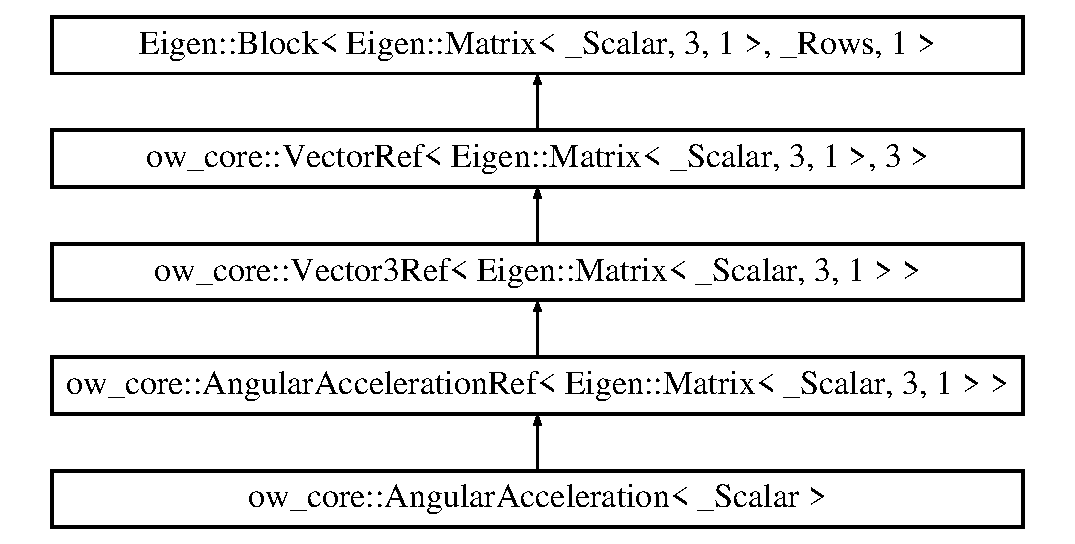
\includegraphics[height=5.000000cm]{d2/d33/classow__core_1_1AngularAcceleration}
\end{center}
\end{figure}
\subsection*{Public Types}
\begin{DoxyCompactItemize}
\item 
typedef \+\_\+\+Scalar {\bfseries Scalar}\hypertarget{classow__core_1_1AngularAcceleration_ae8780d9abd70134aef459b9bf3b4a414}{}\label{classow__core_1_1AngularAcceleration_ae8780d9abd70134aef459b9bf3b4a414}

\item 
typedef Eigen\+::\+Matrix$<$ Scalar, 3, 1 $>$ {\bfseries Derived}\hypertarget{classow__core_1_1AngularAcceleration_a4ab24bb9f976fba36d1c35ca91ff4f95}{}\label{classow__core_1_1AngularAcceleration_a4ab24bb9f976fba36d1c35ca91ff4f95}

\item 
typedef \hyperlink{classow__core_1_1AngularAccelerationRef}{Angular\+Acceleration\+Ref}$<$ Derived $>$ {\bfseries Base}\hypertarget{classow__core_1_1AngularAcceleration_a7c46512723a6c5f857bc621e99d61cc5}{}\label{classow__core_1_1AngularAcceleration_a7c46512723a6c5f857bc621e99d61cc5}

\end{DoxyCompactItemize}
\subsection*{Public Member Functions}
\begin{DoxyCompactItemize}
\item 
\hyperlink{classow__core_1_1AngularAcceleration_a24b5ba9e746b1056afa617dc35cc1909}{Angular\+Acceleration} ()\hypertarget{classow__core_1_1AngularAcceleration_a24b5ba9e746b1056afa617dc35cc1909}{}\label{classow__core_1_1AngularAcceleration_a24b5ba9e746b1056afa617dc35cc1909}

\begin{DoxyCompactList}\small\item\em Default Constructor. \end{DoxyCompactList}\item 
\hyperlink{classow__core_1_1AngularAcceleration_a3091dac3c3ba75b079b2f38675c735fb}{Angular\+Acceleration} (const Scalar \&x, const Scalar \&y, const Scalar \&z)\hypertarget{classow__core_1_1AngularAcceleration_a3091dac3c3ba75b079b2f38675c735fb}{}\label{classow__core_1_1AngularAcceleration_a3091dac3c3ba75b079b2f38675c735fb}

\begin{DoxyCompactList}\small\item\em Assignment from Scalar values. \end{DoxyCompactList}\item 
{\footnotesize template$<$typename Other\+Derived $>$ }\\\hyperlink{classow__core_1_1AngularAcceleration_a2d004049ef71a1522e61bce3ff5e4bfc}{Angular\+Acceleration} (const Eigen\+::\+Eigen\+Base$<$ Other\+Derived $>$ \&other)
\begin{DoxyCompactList}\small\item\em Copy constructor. \end{DoxyCompactList}\end{DoxyCompactItemize}
\subsection*{Protected Attributes}
\begin{DoxyCompactItemize}
\item 
Derived {\bfseries data\+\_\+}\hypertarget{classow__core_1_1AngularAcceleration_a799354c6062ef185d2f284ec9c483509}{}\label{classow__core_1_1AngularAcceleration_a799354c6062ef185d2f284ec9c483509}

\end{DoxyCompactItemize}


\subsection{Detailed Description}
\subsubsection*{template$<$typename \+\_\+\+Scalar$>$\\*
class ow\+\_\+core\+::\+Angular\+Acceleration$<$ \+\_\+\+Scalar $>$}

The \hyperlink{classow__core_1_1AngularAcceleration}{Angular\+Acceleration} class. 

The \hyperlink{classow__core_1_1AngularAcceleration}{Angular\+Acceleration} is of type Eigen\+::\+Vector3 and is represented by the math symbol $\mathbf{\alpha}$. 

\subsection{Constructor \& Destructor Documentation}
\index{ow\+\_\+core\+::\+Angular\+Acceleration@{ow\+\_\+core\+::\+Angular\+Acceleration}!Angular\+Acceleration@{Angular\+Acceleration}}
\index{Angular\+Acceleration@{Angular\+Acceleration}!ow\+\_\+core\+::\+Angular\+Acceleration@{ow\+\_\+core\+::\+Angular\+Acceleration}}
\subsubsection[{\texorpdfstring{Angular\+Acceleration(const Eigen\+::\+Eigen\+Base$<$ Other\+Derived $>$ \&other)}{AngularAcceleration(const Eigen::EigenBase< OtherDerived > &other)}}]{\setlength{\rightskip}{0pt plus 5cm}template$<$typename \+\_\+\+Scalar $>$ template$<$typename Other\+Derived $>$ {\bf ow\+\_\+core\+::\+Angular\+Acceleration}$<$ \+\_\+\+Scalar $>$\+::{\bf Angular\+Acceleration} (
\begin{DoxyParamCaption}
\item[{const Eigen\+::\+Eigen\+Base$<$ Other\+Derived $>$ \&}]{other}
\end{DoxyParamCaption}
)\hspace{0.3cm}{\ttfamily [inline]}}\hypertarget{classow__core_1_1AngularAcceleration_a2d004049ef71a1522e61bce3ff5e4bfc}{}\label{classow__core_1_1AngularAcceleration_a2d004049ef71a1522e61bce3ff5e4bfc}


Copy constructor. 

This copy constructor not only works with Eigen matrices but also with their expressions. 

The documentation for this class was generated from the following file\+:\begin{DoxyCompactItemize}
\item 
/home/dean/ros/workspaces/ow\+\_\+test\+\_\+ws/src/ow\+\_\+core/include/ow\+\_\+core/\hyperlink{angular__acceleration_8h}{angular\+\_\+acceleration.\+h}\end{DoxyCompactItemize}

\hypertarget{classow__core_1_1AngularAccelerationRef}{}\section{ow\+\_\+core\+:\+:Angular\+Acceleration\+Ref$<$ \+\_\+\+Derived $>$ Class Template Reference}
\label{classow__core_1_1AngularAccelerationRef}\index{ow\+\_\+core\+::\+Angular\+Acceleration\+Ref$<$ \+\_\+\+Derived $>$@{ow\+\_\+core\+::\+Angular\+Acceleration\+Ref$<$ \+\_\+\+Derived $>$}}


The \hyperlink{classow__core_1_1AngularAccelerationRef}{Angular\+Acceleration\+Ref} class.  




{\ttfamily \#include $<$angular\+\_\+acceleration\+\_\+ref.\+h$>$}

Inheritance diagram for ow\+\_\+core\+:\+:Angular\+Acceleration\+Ref$<$ \+\_\+\+Derived $>$\+:\begin{figure}[H]
\begin{center}
\leavevmode
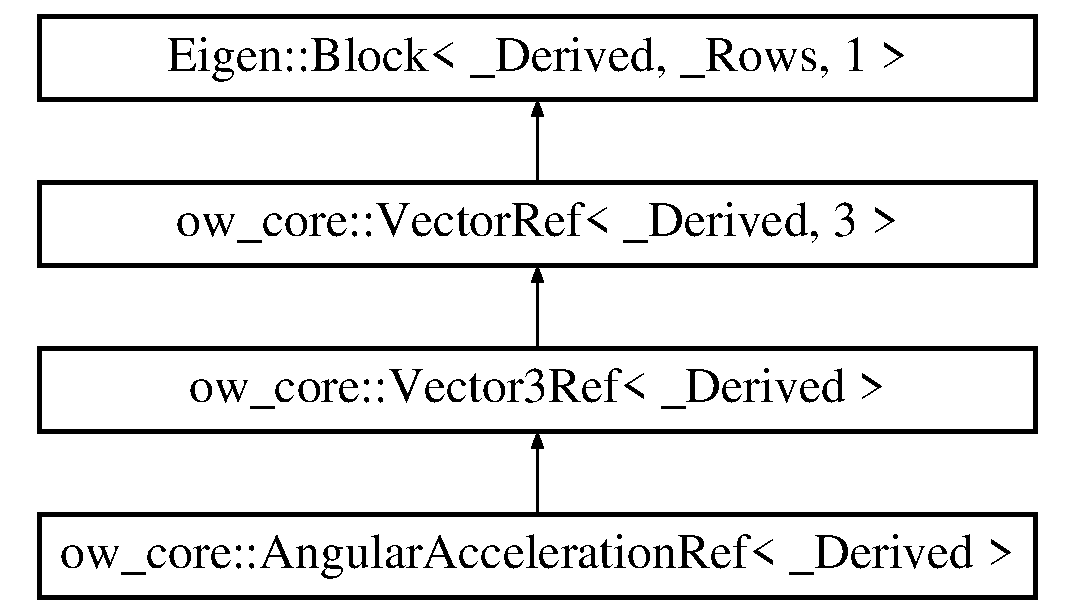
\includegraphics[height=4.000000cm]{d6/d6c/classow__core_1_1AngularAccelerationRef}
\end{center}
\end{figure}
\subsection*{Public Types}
\begin{DoxyCompactItemize}
\item 
typedef \+\_\+\+Derived {\bfseries Derived}\hypertarget{classow__core_1_1AngularAccelerationRef_afa1a59d3353ae26c4b217c5910c3b774}{}\label{classow__core_1_1AngularAccelerationRef_afa1a59d3353ae26c4b217c5910c3b774}

\item 
typedef \hyperlink{classow__core_1_1Vector3Ref}{Vector3\+Ref}$<$ Derived $>$ {\bfseries Base}\hypertarget{classow__core_1_1AngularAccelerationRef_a0019a8fd1b3bb570ae1a6f36b7466558}{}\label{classow__core_1_1AngularAccelerationRef_a0019a8fd1b3bb570ae1a6f36b7466558}

\end{DoxyCompactItemize}
\subsection*{Public Member Functions}
\begin{DoxyCompactItemize}
\item 
\hyperlink{classow__core_1_1AngularAccelerationRef_a5ce015bd30ab9300d7e8255568eb3287}{Angular\+Acceleration\+Ref} (Derived \&ref, int start\+Row=0, int start\+Col=0)
\begin{DoxyCompactList}\small\item\em Default Constructor. \end{DoxyCompactList}\end{DoxyCompactItemize}


\subsection{Detailed Description}
\subsubsection*{template$<$typename \+\_\+\+Derived$>$\\*
class ow\+\_\+core\+::\+Angular\+Acceleration\+Ref$<$ \+\_\+\+Derived $>$}

The \hyperlink{classow__core_1_1AngularAccelerationRef}{Angular\+Acceleration\+Ref} class. 

The \hyperlink{classow__core_1_1AngularAcceleration}{Angular\+Acceleration} is of type Eigen\+::\+Vector3 and is represented by the math symbol $\mathbf{\alpha}$.

References the data of another Eigen type class via Eigen\+::\+Block. 

\subsection{Constructor \& Destructor Documentation}
\index{ow\+\_\+core\+::\+Angular\+Acceleration\+Ref@{ow\+\_\+core\+::\+Angular\+Acceleration\+Ref}!Angular\+Acceleration\+Ref@{Angular\+Acceleration\+Ref}}
\index{Angular\+Acceleration\+Ref@{Angular\+Acceleration\+Ref}!ow\+\_\+core\+::\+Angular\+Acceleration\+Ref@{ow\+\_\+core\+::\+Angular\+Acceleration\+Ref}}
\subsubsection[{\texorpdfstring{Angular\+Acceleration\+Ref(\+Derived \&ref, int start\+Row=0, int start\+Col=0)}{AngularAccelerationRef(Derived &ref, int startRow=0, int startCol=0)}}]{\setlength{\rightskip}{0pt plus 5cm}template$<$typename \+\_\+\+Derived$>$ {\bf ow\+\_\+core\+::\+Angular\+Acceleration\+Ref}$<$ \+\_\+\+Derived $>$\+::{\bf Angular\+Acceleration\+Ref} (
\begin{DoxyParamCaption}
\item[{Derived \&}]{ref, }
\item[{int}]{start\+Row = {\ttfamily 0}, }
\item[{int}]{start\+Col = {\ttfamily 0}}
\end{DoxyParamCaption}
)\hspace{0.3cm}{\ttfamily [inline]}, {\ttfamily [explicit]}}\hypertarget{classow__core_1_1AngularAccelerationRef_a5ce015bd30ab9300d7e8255568eb3287}{}\label{classow__core_1_1AngularAccelerationRef_a5ce015bd30ab9300d7e8255568eb3287}


Default Constructor. 


\begin{DoxyParams}{Parameters}
{\em ref} & the reference to storage Eigen object to access the elements of the \hyperlink{classow__core_1_1AngularVelocity}{Angular\+Velocity} via Eigen\+::\+Block.\\
\hline
{\em start\+Row} & the start index of the row for Eigen\+::\+Block.\\
\hline
{\em start\+Col} & the start index of the column for Eigen\+::\+Block. \\
\hline
\end{DoxyParams}


The documentation for this class was generated from the following file\+:\begin{DoxyCompactItemize}
\item 
/home/dean/ros/workspaces/ow\+\_\+test\+\_\+ws/src/ow\+\_\+core/include/ow\+\_\+core/\hyperlink{angular__acceleration__ref_8h}{angular\+\_\+acceleration\+\_\+ref.\+h}\end{DoxyCompactItemize}

\hypertarget{classow__core_1_1AngularPosition}{}\section{ow\+\_\+core\+:\+:Angular\+Position$<$ \+\_\+\+Scalar $>$ Class Template Reference}
\label{classow__core_1_1AngularPosition}\index{ow\+\_\+core\+::\+Angular\+Position$<$ \+\_\+\+Scalar $>$@{ow\+\_\+core\+::\+Angular\+Position$<$ \+\_\+\+Scalar $>$}}


The \hyperlink{classow__core_1_1AngularPosition}{Angular\+Position} class.  




{\ttfamily \#include $<$angular\+\_\+position.\+h$>$}

Inheritance diagram for ow\+\_\+core\+:\+:Angular\+Position$<$ \+\_\+\+Scalar $>$\+:\begin{figure}[H]
\begin{center}
\leavevmode
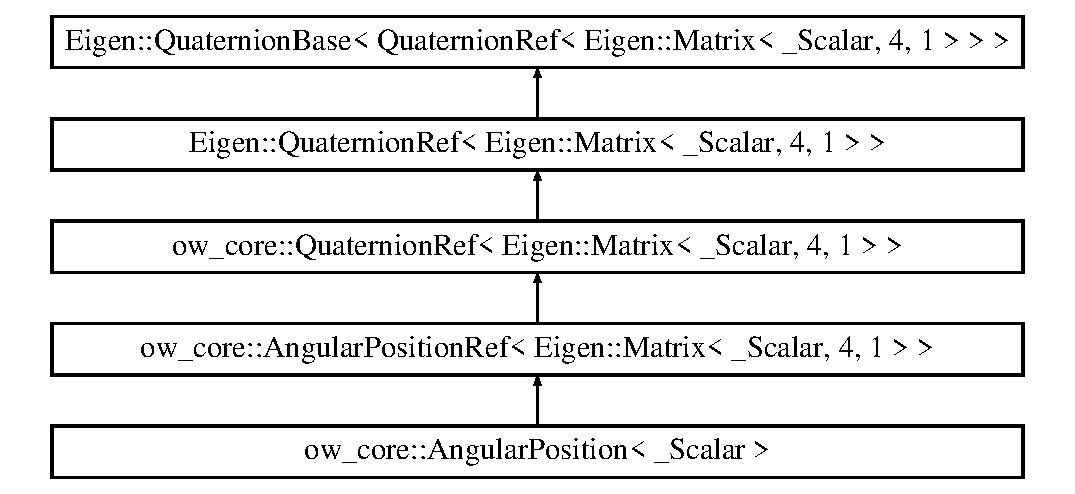
\includegraphics[height=5.000000cm]{d8/d16/classow__core_1_1AngularPosition}
\end{center}
\end{figure}
\subsection*{Public Types}
\begin{DoxyCompactItemize}
\item 
typedef \+\_\+\+Scalar {\bfseries Scalar}\hypertarget{classow__core_1_1AngularPosition_a115f32aed8be3c9a1ae111c7c1a963ff}{}\label{classow__core_1_1AngularPosition_a115f32aed8be3c9a1ae111c7c1a963ff}

\item 
typedef Eigen\+::\+Matrix$<$ Scalar, 4, 1 $>$ {\bfseries Derived}\hypertarget{classow__core_1_1AngularPosition_a4eaba66166c84a3410c31ea2cb3494c2}{}\label{classow__core_1_1AngularPosition_a4eaba66166c84a3410c31ea2cb3494c2}

\item 
typedef \hyperlink{classow__core_1_1AngularPositionRef}{Angular\+Position\+Ref}$<$ Derived $>$ {\bfseries Base}\hypertarget{classow__core_1_1AngularPosition_a1894a069c1ad7c9c3f93a7d40133e38d}{}\label{classow__core_1_1AngularPosition_a1894a069c1ad7c9c3f93a7d40133e38d}

\end{DoxyCompactItemize}
\subsection*{Public Member Functions}
\begin{DoxyCompactItemize}
\item 
\hyperlink{classow__core_1_1AngularPosition_a57812720a8d02ece9fff081bcb67603a}{Angular\+Position} ()\hypertarget{classow__core_1_1AngularPosition_a57812720a8d02ece9fff081bcb67603a}{}\label{classow__core_1_1AngularPosition_a57812720a8d02ece9fff081bcb67603a}

\begin{DoxyCompactList}\small\item\em Default Constructor. \end{DoxyCompactList}\item 
\hyperlink{classow__core_1_1AngularPosition_ab219dc83bafbd964f7fd8bdc2ae9d846}{Angular\+Position} (const Scalar \&w, const Scalar \&x, const Scalar \&y, const Scalar \&z)
\begin{DoxyCompactList}\small\item\em Assignment from Scalar values. \end{DoxyCompactList}\item 
{\footnotesize template$<$typename Other\+Derived $>$ }\\\hyperlink{classow__core_1_1AngularPosition_aaf802dfe295148bc8921e0d8671fc4e9}{Angular\+Position} (const Eigen\+::\+Eigen\+Base$<$ Other\+Derived $>$ \&other)\hypertarget{classow__core_1_1AngularPosition_aaf802dfe295148bc8921e0d8671fc4e9}{}\label{classow__core_1_1AngularPosition_aaf802dfe295148bc8921e0d8671fc4e9}

\begin{DoxyCompactList}\small\item\em Copy constructor from Eigen\+Base. \end{DoxyCompactList}\item 
{\footnotesize template$<$typename Other\+Derived $>$ }\\\hyperlink{classow__core_1_1AngularPosition_ad0343736cc6a1fc3953294727b3721d6}{Angular\+Position} (const Eigen\+::\+Quaternion\+Base$<$ Other\+Derived $>$ \&other)\hypertarget{classow__core_1_1AngularPosition_ad0343736cc6a1fc3953294727b3721d6}{}\label{classow__core_1_1AngularPosition_ad0343736cc6a1fc3953294727b3721d6}

\begin{DoxyCompactList}\small\item\em Copy constructor from Quaternion\+Base. \end{DoxyCompactList}\end{DoxyCompactItemize}
\subsection*{Protected Attributes}
\begin{DoxyCompactItemize}
\item 
Derived {\bfseries data\+\_\+}\hypertarget{classow__core_1_1AngularPosition_a1f581a310708ff8733837d9d1ef553a2}{}\label{classow__core_1_1AngularPosition_a1f581a310708ff8733837d9d1ef553a2}

\end{DoxyCompactItemize}


\subsection{Detailed Description}
\subsubsection*{template$<$typename \+\_\+\+Scalar$>$\\*
class ow\+\_\+core\+::\+Angular\+Position$<$ \+\_\+\+Scalar $>$}

The \hyperlink{classow__core_1_1AngularPosition}{Angular\+Position} class. 

The \hyperlink{classow__core_1_1AngularPosition}{Angular\+Position} is of type Eigen\+::\+Quaternion and is represented by the math symbol $\mathbf{Q}$. 

\subsection{Constructor \& Destructor Documentation}
\index{ow\+\_\+core\+::\+Angular\+Position@{ow\+\_\+core\+::\+Angular\+Position}!Angular\+Position@{Angular\+Position}}
\index{Angular\+Position@{Angular\+Position}!ow\+\_\+core\+::\+Angular\+Position@{ow\+\_\+core\+::\+Angular\+Position}}
\subsubsection[{\texorpdfstring{Angular\+Position(const Scalar \&w, const Scalar \&x, const Scalar \&y, const Scalar \&z)}{AngularPosition(const Scalar &w, const Scalar &x, const Scalar &y, const Scalar &z)}}]{\setlength{\rightskip}{0pt plus 5cm}template$<$typename \+\_\+\+Scalar$>$ {\bf ow\+\_\+core\+::\+Angular\+Position}$<$ \+\_\+\+Scalar $>$\+::{\bf Angular\+Position} (
\begin{DoxyParamCaption}
\item[{const Scalar \&}]{w, }
\item[{const Scalar \&}]{x, }
\item[{const Scalar \&}]{y, }
\item[{const Scalar \&}]{z}
\end{DoxyParamCaption}
)\hspace{0.3cm}{\ttfamily [inline]}}\hypertarget{classow__core_1_1AngularPosition_ab219dc83bafbd964f7fd8bdc2ae9d846}{}\label{classow__core_1_1AngularPosition_ab219dc83bafbd964f7fd8bdc2ae9d846}


Assignment from Scalar values. 

Internally the coefficients are stored in the following order\+: \mbox{[}x, y, z, w\mbox{]} 

The documentation for this class was generated from the following file\+:\begin{DoxyCompactItemize}
\item 
/home/dean/ros/workspaces/ow\+\_\+test\+\_\+ws/src/ow\+\_\+core/include/ow\+\_\+core/\hyperlink{angular__position_8h}{angular\+\_\+position.\+h}\end{DoxyCompactItemize}

\hypertarget{classow__core_1_1AngularPositionRef}{}\section{ow\+\_\+core\+:\+:Angular\+Position\+Ref$<$ \+\_\+\+Derived $>$ Class Template Reference}
\label{classow__core_1_1AngularPositionRef}\index{ow\+\_\+core\+::\+Angular\+Position\+Ref$<$ \+\_\+\+Derived $>$@{ow\+\_\+core\+::\+Angular\+Position\+Ref$<$ \+\_\+\+Derived $>$}}


The \hyperlink{classow__core_1_1AngularPositionRef}{Angular\+Position\+Ref} class.  




{\ttfamily \#include $<$angular\+\_\+position\+\_\+ref.\+h$>$}

Inheritance diagram for ow\+\_\+core\+:\+:Angular\+Position\+Ref$<$ \+\_\+\+Derived $>$\+:\begin{figure}[H]
\begin{center}
\leavevmode
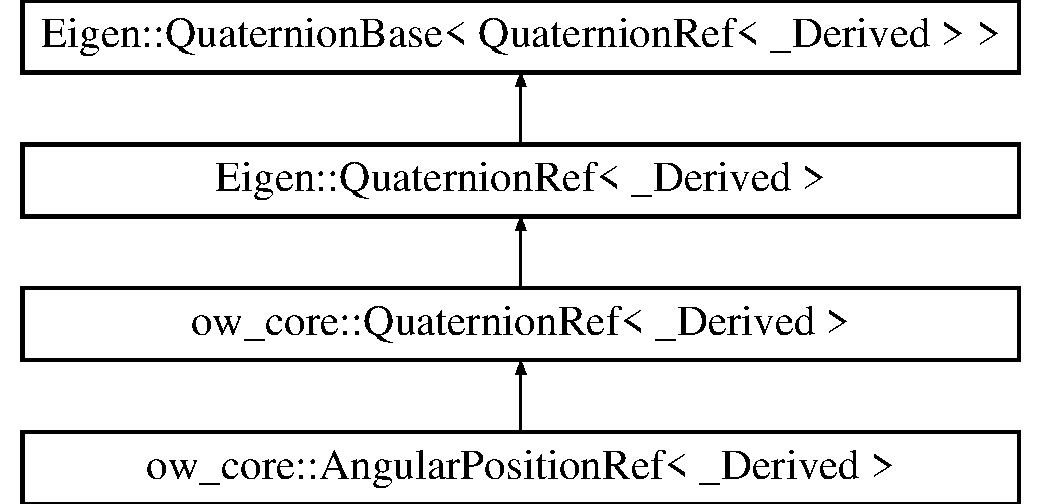
\includegraphics[height=4.000000cm]{db/d23/classow__core_1_1AngularPositionRef}
\end{center}
\end{figure}
\subsection*{Public Types}
\begin{DoxyCompactItemize}
\item 
typedef \+\_\+\+Derived {\bfseries Derived}\hypertarget{classow__core_1_1AngularPositionRef_a66f7abe85130a4a26a8fd6a566dc5423}{}\label{classow__core_1_1AngularPositionRef_a66f7abe85130a4a26a8fd6a566dc5423}

\item 
typedef \hyperlink{classow__core_1_1QuaternionRef}{Quaternion\+Ref}$<$ Derived $>$ {\bfseries Base}\hypertarget{classow__core_1_1AngularPositionRef_a8332ab03e73f58c27f92c170894d67b7}{}\label{classow__core_1_1AngularPositionRef_a8332ab03e73f58c27f92c170894d67b7}

\end{DoxyCompactItemize}
\subsection*{Public Member Functions}
\begin{DoxyCompactItemize}
\item 
\hyperlink{classow__core_1_1AngularPositionRef_aee0bb9a66511067009504119ffb5f2cc}{Angular\+Position\+Ref} (Derived \&ref, int start\+Row=0, int start\+Col=0)
\begin{DoxyCompactList}\small\item\em Default Constructor. \end{DoxyCompactList}\item 
void \hyperlink{classow__core_1_1AngularPositionRef_a0c67d3e57001c3f4b47983c6e2113410}{operator=} (const tf\+::\+Quaternion \&q)
\begin{DoxyCompactList}\small\item\em Assignment of tf\+::\+Quaternion. \end{DoxyCompactList}\item 
void \hyperlink{classow__core_1_1AngularPositionRef_a0698779622d693951e2c9c621c6c35f7}{operator=} (const geometry\+\_\+msgs\+::\+Quaternion \&q)
\begin{DoxyCompactList}\small\item\em Assignment of geometry\+\_\+msgs\+::\+Quaternion. \end{DoxyCompactList}\item 
void \hyperlink{classow__core_1_1AngularPositionRef_ae1e71403873af767a56ef0257e76b683}{operator=} (const tf\+::\+Matrix3x3 \&other)\hypertarget{classow__core_1_1AngularPositionRef_ae1e71403873af767a56ef0257e76b683}{}\label{classow__core_1_1AngularPositionRef_ae1e71403873af767a56ef0257e76b683}

\begin{DoxyCompactList}\small\item\em Assignment of tf\+::\+Matrix3x3. \end{DoxyCompactList}\item 
\hyperlink{classow__core_1_1AngularPositionRef_a93616aede6f30d7721f5b83f02f96d0d}{operator tf\+::\+Quaternion} () const \hypertarget{classow__core_1_1AngularPositionRef_a93616aede6f30d7721f5b83f02f96d0d}{}\label{classow__core_1_1AngularPositionRef_a93616aede6f30d7721f5b83f02f96d0d}

\begin{DoxyCompactList}\small\item\em Conversion to tf\+::\+Quaternion. \end{DoxyCompactList}\item 
\hyperlink{classow__core_1_1AngularPositionRef_ac36a2117df9ad13c8898c3336294c7d1}{operator geometry\+\_\+msgs\+::\+Quaternion} () const \hypertarget{classow__core_1_1AngularPositionRef_ac36a2117df9ad13c8898c3336294c7d1}{}\label{classow__core_1_1AngularPositionRef_ac36a2117df9ad13c8898c3336294c7d1}

\begin{DoxyCompactList}\small\item\em Conversion to geometry\+\_\+msgs\+::\+Quaternion. \end{DoxyCompactList}\item 
\hyperlink{classow__core_1_1AngularPositionRef_a6bc0dc8d7cb5cf31f264024ef1071686}{operator tf\+::\+Matrix3x3} () const \hypertarget{classow__core_1_1AngularPositionRef_a6bc0dc8d7cb5cf31f264024ef1071686}{}\label{classow__core_1_1AngularPositionRef_a6bc0dc8d7cb5cf31f264024ef1071686}

\begin{DoxyCompactList}\small\item\em Conversion to tf\+::\+Matrix3x3. \end{DoxyCompactList}\item 
tf\+::\+Quaternion \hyperlink{classow__core_1_1AngularPositionRef_a7c2c2d8e595fa548b34a4f2f2a093f9c}{to\+Quaternion\+TF} ()\hypertarget{classow__core_1_1AngularPositionRef_a7c2c2d8e595fa548b34a4f2f2a093f9c}{}\label{classow__core_1_1AngularPositionRef_a7c2c2d8e595fa548b34a4f2f2a093f9c}

\begin{DoxyCompactList}\small\item\em Conversion to tf\+::\+Quaternion. \end{DoxyCompactList}\item 
geometry\+\_\+msgs\+::\+Quaternion \hyperlink{classow__core_1_1AngularPositionRef_af3fa191a6e35e4e55f3cc8730936e5da}{to\+Quaternion\+Msg} ()\hypertarget{classow__core_1_1AngularPositionRef_af3fa191a6e35e4e55f3cc8730936e5da}{}\label{classow__core_1_1AngularPositionRef_af3fa191a6e35e4e55f3cc8730936e5da}

\begin{DoxyCompactList}\small\item\em Conversion to geometry\+\_\+msgs\+::\+Quaternion. \end{DoxyCompactList}\item 
tf\+::\+Matrix3x3 \hyperlink{classow__core_1_1AngularPositionRef_a84c7eb3a2bf5883c692ef40b672988fb}{to\+Matrix\+TF} ()\hypertarget{classow__core_1_1AngularPositionRef_a84c7eb3a2bf5883c692ef40b672988fb}{}\label{classow__core_1_1AngularPositionRef_a84c7eb3a2bf5883c692ef40b672988fb}

\begin{DoxyCompactList}\small\item\em Conversion to tf\+::\+Matrix3x3. \end{DoxyCompactList}\end{DoxyCompactItemize}
\subsection*{Additional Inherited Members}


\subsection{Detailed Description}
\subsubsection*{template$<$typename \+\_\+\+Derived$>$\\*
class ow\+\_\+core\+::\+Angular\+Position\+Ref$<$ \+\_\+\+Derived $>$}

The \hyperlink{classow__core_1_1AngularPositionRef}{Angular\+Position\+Ref} class. 

The \hyperlink{classow__core_1_1AngularPosition}{Angular\+Position} is of type Eigen\+::\+Quaternion and is represented by the math symbol $\mathbf{Q}$.

References the data of another Eigen type class via Eigen\+:Block.

We need this special type to get the behavior of Eigen\+::\+Quaternion and add specific new functionality. 

\subsection{Constructor \& Destructor Documentation}
\index{ow\+\_\+core\+::\+Angular\+Position\+Ref@{ow\+\_\+core\+::\+Angular\+Position\+Ref}!Angular\+Position\+Ref@{Angular\+Position\+Ref}}
\index{Angular\+Position\+Ref@{Angular\+Position\+Ref}!ow\+\_\+core\+::\+Angular\+Position\+Ref@{ow\+\_\+core\+::\+Angular\+Position\+Ref}}
\subsubsection[{\texorpdfstring{Angular\+Position\+Ref(\+Derived \&ref, int start\+Row=0, int start\+Col=0)}{AngularPositionRef(Derived &ref, int startRow=0, int startCol=0)}}]{\setlength{\rightskip}{0pt plus 5cm}template$<$typename \+\_\+\+Derived$>$ {\bf ow\+\_\+core\+::\+Angular\+Position\+Ref}$<$ \+\_\+\+Derived $>$\+::{\bf Angular\+Position\+Ref} (
\begin{DoxyParamCaption}
\item[{Derived \&}]{ref, }
\item[{int}]{start\+Row = {\ttfamily 0}, }
\item[{int}]{start\+Col = {\ttfamily 0}}
\end{DoxyParamCaption}
)\hspace{0.3cm}{\ttfamily [inline]}, {\ttfamily [explicit]}}\hypertarget{classow__core_1_1AngularPositionRef_aee0bb9a66511067009504119ffb5f2cc}{}\label{classow__core_1_1AngularPositionRef_aee0bb9a66511067009504119ffb5f2cc}


Default Constructor. 


\begin{DoxyParams}{Parameters}
{\em ref} & the reference to storage Eigen object to access the elements of the quaternion via Eigen\+::\+Block.\\
\hline
{\em start\+Row} & the start index of the row for Eigen\+::\+Block.\\
\hline
{\em start\+Col} & the start index of the column for Eigen\+::\+Block. \\
\hline
\end{DoxyParams}


\subsection{Member Function Documentation}
\index{ow\+\_\+core\+::\+Angular\+Position\+Ref@{ow\+\_\+core\+::\+Angular\+Position\+Ref}!operator=@{operator=}}
\index{operator=@{operator=}!ow\+\_\+core\+::\+Angular\+Position\+Ref@{ow\+\_\+core\+::\+Angular\+Position\+Ref}}
\subsubsection[{\texorpdfstring{operator=(const tf\+::\+Quaternion \&q)}{operator=(const tf::Quaternion &q)}}]{\setlength{\rightskip}{0pt plus 5cm}template$<$typename \+\_\+\+Derived$>$ void {\bf ow\+\_\+core\+::\+Angular\+Position\+Ref}$<$ \+\_\+\+Derived $>$\+::operator= (
\begin{DoxyParamCaption}
\item[{const tf\+::\+Quaternion \&}]{q}
\end{DoxyParamCaption}
)\hspace{0.3cm}{\ttfamily [inline]}}\hypertarget{classow__core_1_1AngularPositionRef_a0c67d3e57001c3f4b47983c6e2113410}{}\label{classow__core_1_1AngularPositionRef_a0c67d3e57001c3f4b47983c6e2113410}


Assignment of tf\+::\+Quaternion. 

\begin{DoxyRefDesc}{Todo}
\item[\hyperlink{todo__todo000001}{Todo}]Maybe call a static converion function.\end{DoxyRefDesc}
\index{ow\+\_\+core\+::\+Angular\+Position\+Ref@{ow\+\_\+core\+::\+Angular\+Position\+Ref}!operator=@{operator=}}
\index{operator=@{operator=}!ow\+\_\+core\+::\+Angular\+Position\+Ref@{ow\+\_\+core\+::\+Angular\+Position\+Ref}}
\subsubsection[{\texorpdfstring{operator=(const geometry\+\_\+msgs\+::\+Quaternion \&q)}{operator=(const geometry_msgs::Quaternion &q)}}]{\setlength{\rightskip}{0pt plus 5cm}template$<$typename \+\_\+\+Derived$>$ void {\bf ow\+\_\+core\+::\+Angular\+Position\+Ref}$<$ \+\_\+\+Derived $>$\+::operator= (
\begin{DoxyParamCaption}
\item[{const geometry\+\_\+msgs\+::\+Quaternion \&}]{q}
\end{DoxyParamCaption}
)\hspace{0.3cm}{\ttfamily [inline]}}\hypertarget{classow__core_1_1AngularPositionRef_a0698779622d693951e2c9c621c6c35f7}{}\label{classow__core_1_1AngularPositionRef_a0698779622d693951e2c9c621c6c35f7}


Assignment of geometry\+\_\+msgs\+::\+Quaternion. 

\begin{DoxyRefDesc}{Bug}
\item[\hyperlink{bug__bug000001}{Bug}]This is a test bug to test the listing. Remove! \end{DoxyRefDesc}


The documentation for this class was generated from the following file\+:\begin{DoxyCompactItemize}
\item 
/home/dean/ros/workspaces/ow\+\_\+test\+\_\+ws/src/ow\+\_\+core/include/ow\+\_\+core/\hyperlink{angular__position__ref_8h}{angular\+\_\+position\+\_\+ref.\+h}\end{DoxyCompactItemize}

\hypertarget{classow__core_1_1AngularVelocity}{}\section{ow\+\_\+core\+:\+:Angular\+Velocity$<$ \+\_\+\+Scalar $>$ Class Template Reference}
\label{classow__core_1_1AngularVelocity}\index{ow\+\_\+core\+::\+Angular\+Velocity$<$ \+\_\+\+Scalar $>$@{ow\+\_\+core\+::\+Angular\+Velocity$<$ \+\_\+\+Scalar $>$}}


The \hyperlink{classow__core_1_1AngularVelocity}{Angular\+Velocity} class.  




{\ttfamily \#include $<$angular\+\_\+velocity.\+h$>$}

Inheritance diagram for ow\+\_\+core\+:\+:Angular\+Velocity$<$ \+\_\+\+Scalar $>$\+:\begin{figure}[H]
\begin{center}
\leavevmode
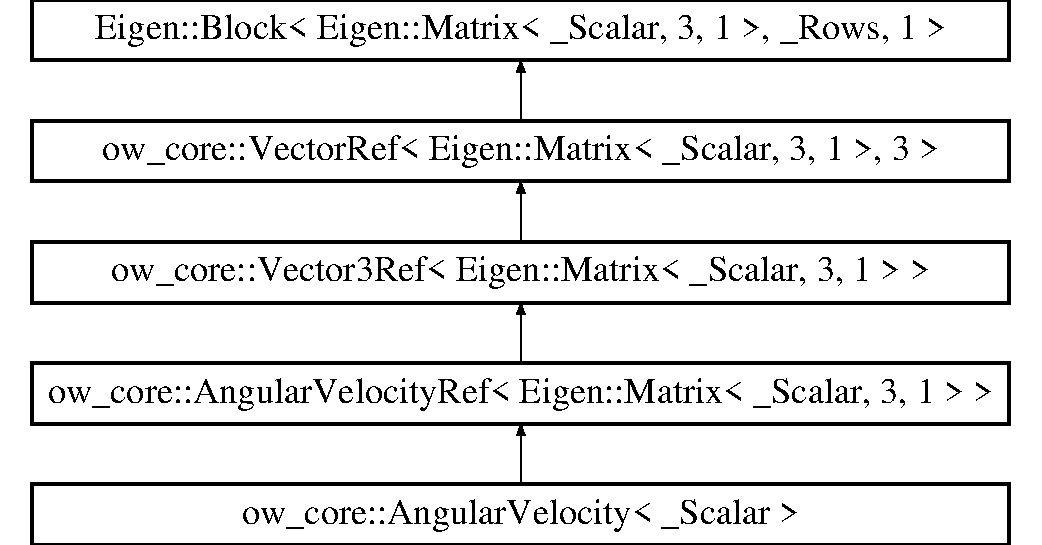
\includegraphics[height=5.000000cm]{d2/da5/classow__core_1_1AngularVelocity}
\end{center}
\end{figure}
\subsection*{Public Types}
\begin{DoxyCompactItemize}
\item 
typedef \+\_\+\+Scalar {\bfseries Scalar}\hypertarget{classow__core_1_1AngularVelocity_ae9c8b95a9177664cf39bd57d667a0fce}{}\label{classow__core_1_1AngularVelocity_ae9c8b95a9177664cf39bd57d667a0fce}

\item 
typedef Eigen\+::\+Matrix$<$ \+\_\+\+Scalar, 3, 1 $>$ {\bfseries Derived}\hypertarget{classow__core_1_1AngularVelocity_a68c6384723283174f366f4faf4693ceb}{}\label{classow__core_1_1AngularVelocity_a68c6384723283174f366f4faf4693ceb}

\item 
typedef \hyperlink{classow__core_1_1AngularVelocityRef}{Angular\+Velocity\+Ref}$<$ Derived $>$ {\bfseries Base}\hypertarget{classow__core_1_1AngularVelocity_a8490799ea74a7119140dd3c32007f78c}{}\label{classow__core_1_1AngularVelocity_a8490799ea74a7119140dd3c32007f78c}

\end{DoxyCompactItemize}
\subsection*{Public Member Functions}
\begin{DoxyCompactItemize}
\item 
\hyperlink{classow__core_1_1AngularVelocity_a4646f848b302b5b4396f5b9a51ffbf8e}{Angular\+Velocity} ()\hypertarget{classow__core_1_1AngularVelocity_a4646f848b302b5b4396f5b9a51ffbf8e}{}\label{classow__core_1_1AngularVelocity_a4646f848b302b5b4396f5b9a51ffbf8e}

\begin{DoxyCompactList}\small\item\em Default Constructor. \end{DoxyCompactList}\item 
\hyperlink{classow__core_1_1AngularVelocity_ad30b2ef68b80c738d78e7898cb017412}{Angular\+Velocity} (const Scalar \&x, const Scalar \&y, const Scalar \&z)\hypertarget{classow__core_1_1AngularVelocity_ad30b2ef68b80c738d78e7898cb017412}{}\label{classow__core_1_1AngularVelocity_ad30b2ef68b80c738d78e7898cb017412}

\begin{DoxyCompactList}\small\item\em Assignment from Scalar values. \end{DoxyCompactList}\item 
{\footnotesize template$<$typename Other\+Derived $>$ }\\\hyperlink{classow__core_1_1AngularVelocity_a711e58379cd2a989339dfd583c9ca999}{Angular\+Velocity} (const Eigen\+::\+Eigen\+Base$<$ Other\+Derived $>$ \&other)
\begin{DoxyCompactList}\small\item\em Copy constructor. \end{DoxyCompactList}\end{DoxyCompactItemize}
\subsection*{Protected Attributes}
\begin{DoxyCompactItemize}
\item 
Derived {\bfseries data\+\_\+}\hypertarget{classow__core_1_1AngularVelocity_acf41236c893aea3624734214dab971ae}{}\label{classow__core_1_1AngularVelocity_acf41236c893aea3624734214dab971ae}

\end{DoxyCompactItemize}


\subsection{Detailed Description}
\subsubsection*{template$<$typename \+\_\+\+Scalar$>$\\*
class ow\+\_\+core\+::\+Angular\+Velocity$<$ \+\_\+\+Scalar $>$}

The \hyperlink{classow__core_1_1AngularVelocity}{Angular\+Velocity} class. 

The \hyperlink{classow__core_1_1AngularVelocity}{Angular\+Velocity} is of type Eigen\+::\+Vector3 and is represented by the math symbol $\mathbf{\omega}$. 

\subsection{Constructor \& Destructor Documentation}
\index{ow\+\_\+core\+::\+Angular\+Velocity@{ow\+\_\+core\+::\+Angular\+Velocity}!Angular\+Velocity@{Angular\+Velocity}}
\index{Angular\+Velocity@{Angular\+Velocity}!ow\+\_\+core\+::\+Angular\+Velocity@{ow\+\_\+core\+::\+Angular\+Velocity}}
\subsubsection[{\texorpdfstring{Angular\+Velocity(const Eigen\+::\+Eigen\+Base$<$ Other\+Derived $>$ \&other)}{AngularVelocity(const Eigen::EigenBase< OtherDerived > &other)}}]{\setlength{\rightskip}{0pt plus 5cm}template$<$typename \+\_\+\+Scalar$>$ template$<$typename Other\+Derived $>$ {\bf ow\+\_\+core\+::\+Angular\+Velocity}$<$ \+\_\+\+Scalar $>$\+::{\bf Angular\+Velocity} (
\begin{DoxyParamCaption}
\item[{const Eigen\+::\+Eigen\+Base$<$ Other\+Derived $>$ \&}]{other}
\end{DoxyParamCaption}
)\hspace{0.3cm}{\ttfamily [inline]}}\hypertarget{classow__core_1_1AngularVelocity_a711e58379cd2a989339dfd583c9ca999}{}\label{classow__core_1_1AngularVelocity_a711e58379cd2a989339dfd583c9ca999}


Copy constructor. 

This copy constructor not only works with Eigen matrices but also with their expressions. 

The documentation for this class was generated from the following file\+:\begin{DoxyCompactItemize}
\item 
/home/dean/ros/workspaces/ow\+\_\+test\+\_\+ws/src/ow\+\_\+core/include/ow\+\_\+core/\hyperlink{angular__velocity_8h}{angular\+\_\+velocity.\+h}\end{DoxyCompactItemize}

\hypertarget{classow__core_1_1AngularVelocityRef}{}\section{ow\+\_\+core\+:\+:Angular\+Velocity\+Ref$<$ \+\_\+\+Derived $>$ Class Template Reference}
\label{classow__core_1_1AngularVelocityRef}\index{ow\+\_\+core\+::\+Angular\+Velocity\+Ref$<$ \+\_\+\+Derived $>$@{ow\+\_\+core\+::\+Angular\+Velocity\+Ref$<$ \+\_\+\+Derived $>$}}


The \hyperlink{classow__core_1_1AngularVelocityRef}{Angular\+Velocity\+Ref} class.  




{\ttfamily \#include $<$angular\+\_\+velocity\+\_\+ref.\+h$>$}

Inheritance diagram for ow\+\_\+core\+:\+:Angular\+Velocity\+Ref$<$ \+\_\+\+Derived $>$\+:\begin{figure}[H]
\begin{center}
\leavevmode
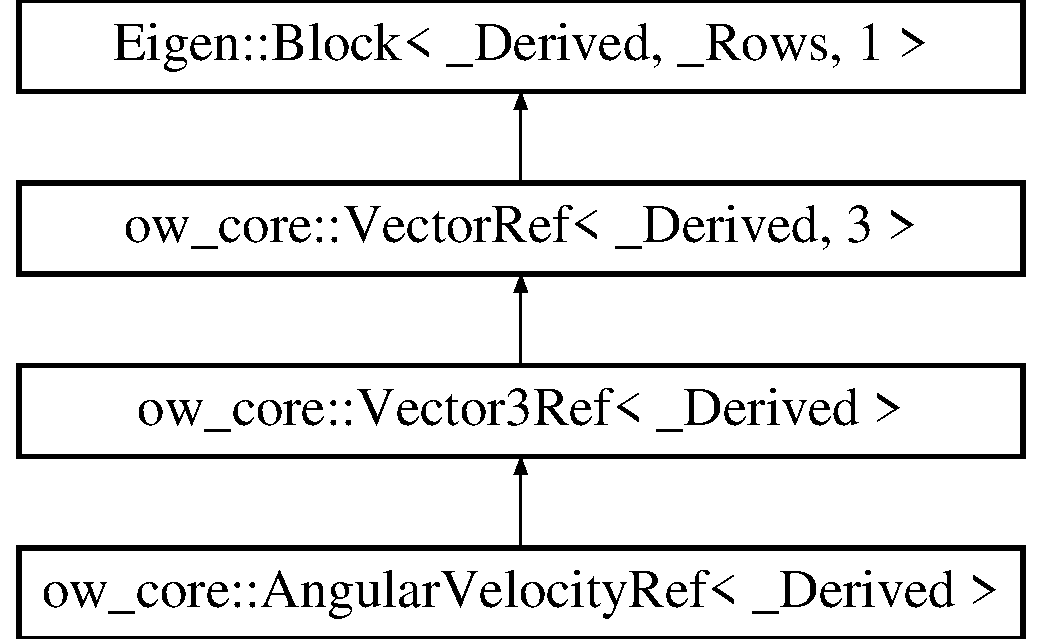
\includegraphics[height=4.000000cm]{de/d7d/classow__core_1_1AngularVelocityRef}
\end{center}
\end{figure}
\subsection*{Public Types}
\begin{DoxyCompactItemize}
\item 
typedef \+\_\+\+Derived {\bfseries Derived}\hypertarget{classow__core_1_1AngularVelocityRef_a05048cc839f03a8b0a013fd5b92aec21}{}\label{classow__core_1_1AngularVelocityRef_a05048cc839f03a8b0a013fd5b92aec21}

\item 
typedef \hyperlink{classow__core_1_1Vector3Ref}{Vector3\+Ref}$<$ Derived $>$ {\bfseries Base}\hypertarget{classow__core_1_1AngularVelocityRef_af26b8bcb21042e6a777eb35a59f4ee2a}{}\label{classow__core_1_1AngularVelocityRef_af26b8bcb21042e6a777eb35a59f4ee2a}

\end{DoxyCompactItemize}
\subsection*{Public Member Functions}
\begin{DoxyCompactItemize}
\item 
\hyperlink{classow__core_1_1AngularVelocityRef_a683f548b84149917945be19fcf197fca}{Angular\+Velocity\+Ref} (Derived \&ref, int start\+Row=0, int start\+Col=0)
\begin{DoxyCompactList}\small\item\em Default Constructor. \end{DoxyCompactList}\end{DoxyCompactItemize}


\subsection{Detailed Description}
\subsubsection*{template$<$typename \+\_\+\+Derived$>$\\*
class ow\+\_\+core\+::\+Angular\+Velocity\+Ref$<$ \+\_\+\+Derived $>$}

The \hyperlink{classow__core_1_1AngularVelocityRef}{Angular\+Velocity\+Ref} class. 

The \hyperlink{classow__core_1_1AngularVelocityRef}{Angular\+Velocity\+Ref} is of type Eigen\+::\+Vector3 and is represented by the math symbol $\mathbf{\omega}$.

References the data of another Eigen type class via Eigen\+::\+Block. 

\subsection{Constructor \& Destructor Documentation}
\index{ow\+\_\+core\+::\+Angular\+Velocity\+Ref@{ow\+\_\+core\+::\+Angular\+Velocity\+Ref}!Angular\+Velocity\+Ref@{Angular\+Velocity\+Ref}}
\index{Angular\+Velocity\+Ref@{Angular\+Velocity\+Ref}!ow\+\_\+core\+::\+Angular\+Velocity\+Ref@{ow\+\_\+core\+::\+Angular\+Velocity\+Ref}}
\subsubsection[{\texorpdfstring{Angular\+Velocity\+Ref(\+Derived \&ref, int start\+Row=0, int start\+Col=0)}{AngularVelocityRef(Derived &ref, int startRow=0, int startCol=0)}}]{\setlength{\rightskip}{0pt plus 5cm}template$<$typename \+\_\+\+Derived$>$ {\bf ow\+\_\+core\+::\+Angular\+Velocity\+Ref}$<$ \+\_\+\+Derived $>$\+::{\bf Angular\+Velocity\+Ref} (
\begin{DoxyParamCaption}
\item[{Derived \&}]{ref, }
\item[{int}]{start\+Row = {\ttfamily 0}, }
\item[{int}]{start\+Col = {\ttfamily 0}}
\end{DoxyParamCaption}
)\hspace{0.3cm}{\ttfamily [inline]}, {\ttfamily [explicit]}}\hypertarget{classow__core_1_1AngularVelocityRef_a683f548b84149917945be19fcf197fca}{}\label{classow__core_1_1AngularVelocityRef_a683f548b84149917945be19fcf197fca}


Default Constructor. 


\begin{DoxyParams}{Parameters}
{\em ref} & the reference to storage Eigen object to access the elements of the \hyperlink{classow__core_1_1AngularVelocity}{Angular\+Velocity} via Eigen\+::\+Block.\\
\hline
{\em start\+Row} & the start index of the row for Eigen\+::\+Block.\\
\hline
{\em start\+Col} & the start index of the column for Eigen\+::\+Block. \\
\hline
\end{DoxyParams}


The documentation for this class was generated from the following file\+:\begin{DoxyCompactItemize}
\item 
/home/dean/ros/workspaces/ow\+\_\+test\+\_\+ws/src/ow\+\_\+core/include/ow\+\_\+core/\hyperlink{angular__velocity__ref_8h}{angular\+\_\+velocity\+\_\+ref.\+h}\end{DoxyCompactItemize}

\hypertarget{classow__core_1_1CartesianAcceleration}{}\section{ow\+\_\+core\+:\+:Cartesian\+Acceleration$<$ \+\_\+\+Scalar $>$ Class Template Reference}
\label{classow__core_1_1CartesianAcceleration}\index{ow\+\_\+core\+::\+Cartesian\+Acceleration$<$ \+\_\+\+Scalar $>$@{ow\+\_\+core\+::\+Cartesian\+Acceleration$<$ \+\_\+\+Scalar $>$}}


The \hyperlink{classow__core_1_1CartesianAcceleration}{Cartesian\+Acceleration} class.  




{\ttfamily \#include $<$cartesian\+\_\+acceleration.\+h$>$}

Inheritance diagram for ow\+\_\+core\+:\+:Cartesian\+Acceleration$<$ \+\_\+\+Scalar $>$\+:\begin{figure}[H]
\begin{center}
\leavevmode
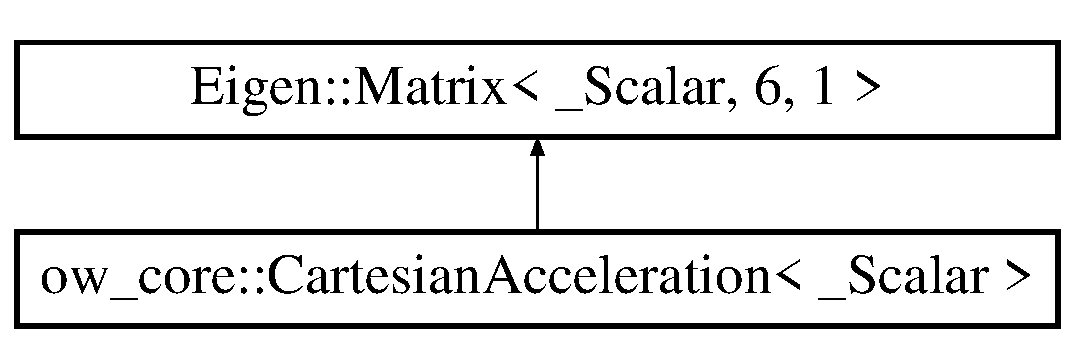
\includegraphics[height=2.000000cm]{df/d67/classow__core_1_1CartesianAcceleration}
\end{center}
\end{figure}
\subsection*{Public Types}
\begin{DoxyCompactItemize}
\item 
typedef \+\_\+\+Scalar {\bfseries Scalar}\hypertarget{classow__core_1_1CartesianAcceleration_aa6c9e5a1a1c66107763255ebd637926d}{}\label{classow__core_1_1CartesianAcceleration_aa6c9e5a1a1c66107763255ebd637926d}

\item 
typedef Eigen\+::\+Matrix$<$ Scalar, 6, 1 $>$ {\bfseries Base}\hypertarget{classow__core_1_1CartesianAcceleration_af0e02dd04a0364641ca0b75b9e9e74de}{}\label{classow__core_1_1CartesianAcceleration_af0e02dd04a0364641ca0b75b9e9e74de}

\end{DoxyCompactItemize}
\subsection*{Public Member Functions}
\begin{DoxyCompactItemize}
\item 
\hyperlink{classow__core_1_1CartesianAcceleration_a53ba452c7479d2fee4ee0285a50e2bbe}{Cartesian\+Acceleration} ()\hypertarget{classow__core_1_1CartesianAcceleration_a53ba452c7479d2fee4ee0285a50e2bbe}{}\label{classow__core_1_1CartesianAcceleration_a53ba452c7479d2fee4ee0285a50e2bbe}

\begin{DoxyCompactList}\small\item\em Default Constructor. \end{DoxyCompactList}\item 
{\footnotesize template$<$typename Other\+Derived $>$ }\\\hyperlink{classow__core_1_1CartesianAcceleration_af7b7922397256f41e7aec8324a4ba319}{Cartesian\+Acceleration} (const Eigen\+::\+Eigen\+Base$<$ Other\+Derived $>$ \&other)
\begin{DoxyCompactList}\small\item\em Copy constructor. \end{DoxyCompactList}\item 
\hyperlink{classow__core_1_1CartesianAcceleration_a00e9ba4327f15f4b81d520ff3c3b665c}{Cartesian\+Acceleration} (const geometry\+\_\+msgs\+::\+Accel \&other)\hypertarget{classow__core_1_1CartesianAcceleration_a00e9ba4327f15f4b81d520ff3c3b665c}{}\label{classow__core_1_1CartesianAcceleration_a00e9ba4327f15f4b81d520ff3c3b665c}

\begin{DoxyCompactList}\small\item\em Copy constructor form geometry\+\_\+msgs\+::\+Accel. \end{DoxyCompactList}\item 
void \hyperlink{classow__core_1_1CartesianAcceleration_ac69817340dd5fd1178764c75707739b9}{operator=} (const geometry\+\_\+msgs\+::\+Accel \&Xpp)\hypertarget{classow__core_1_1CartesianAcceleration_ac69817340dd5fd1178764c75707739b9}{}\label{classow__core_1_1CartesianAcceleration_ac69817340dd5fd1178764c75707739b9}

\begin{DoxyCompactList}\small\item\em Assignment form geometry\+\_\+msgs\+::\+Accel. \end{DoxyCompactList}\item 
\hyperlink{classow__core_1_1CartesianAcceleration_a8e7cd11ab998220f6ea65970605045b7}{operator geometry\+\_\+msgs\+::\+Accel} () const \hypertarget{classow__core_1_1CartesianAcceleration_a8e7cd11ab998220f6ea65970605045b7}{}\label{classow__core_1_1CartesianAcceleration_a8e7cd11ab998220f6ea65970605045b7}

\begin{DoxyCompactList}\small\item\em Conversion to geometry\+\_\+msgs\+::\+Accel. \end{DoxyCompactList}\item 
geometry\+\_\+msgs\+::\+Accel \hyperlink{classow__core_1_1CartesianAcceleration_a127f662e061666d70174897ac315b834}{to\+Accel\+Msg} () const \hypertarget{classow__core_1_1CartesianAcceleration_a127f662e061666d70174897ac315b834}{}\label{classow__core_1_1CartesianAcceleration_a127f662e061666d70174897ac315b834}

\begin{DoxyCompactList}\small\item\em Conversion to geometry\+\_\+msgs\+::\+Twist. \end{DoxyCompactList}\item 
\hyperlink{classow__core_1_1LinearAccelerationRef}{Linear\+Acceleration\+Ref}$<$ Base $>$ \hyperlink{classow__core_1_1CartesianAcceleration_ac814340c03e8322c39db961010f67788}{linear} ()\hypertarget{classow__core_1_1CartesianAcceleration_ac814340c03e8322c39db961010f67788}{}\label{classow__core_1_1CartesianAcceleration_ac814340c03e8322c39db961010f67788}

\begin{DoxyCompactList}\small\item\em access to linear part \end{DoxyCompactList}\item 
\hyperlink{classow__core_1_1LinearAccelerationRef}{Linear\+Acceleration\+Ref}$<$ const Base $>$ \hyperlink{classow__core_1_1CartesianAcceleration_a97e1512119cc3d73c89c50d52a573c07}{linear} () const \hypertarget{classow__core_1_1CartesianAcceleration_a97e1512119cc3d73c89c50d52a573c07}{}\label{classow__core_1_1CartesianAcceleration_a97e1512119cc3d73c89c50d52a573c07}

\begin{DoxyCompactList}\small\item\em const access to linear part \end{DoxyCompactList}\item 
\hyperlink{classow__core_1_1AngularAccelerationRef}{Angular\+Acceleration\+Ref}$<$ Base $>$ \hyperlink{classow__core_1_1CartesianAcceleration_a6569c3763520f857155bca2265cf43c3}{angular} ()\hypertarget{classow__core_1_1CartesianAcceleration_a6569c3763520f857155bca2265cf43c3}{}\label{classow__core_1_1CartesianAcceleration_a6569c3763520f857155bca2265cf43c3}

\begin{DoxyCompactList}\small\item\em access to angular part \end{DoxyCompactList}\item 
\hyperlink{classow__core_1_1AngularAccelerationRef}{Angular\+Acceleration\+Ref}$<$ const Base $>$ \hyperlink{classow__core_1_1CartesianAcceleration_a0573ab2161d29d4956322067f433fa04}{angular} () const \hypertarget{classow__core_1_1CartesianAcceleration_a0573ab2161d29d4956322067f433fa04}{}\label{classow__core_1_1CartesianAcceleration_a0573ab2161d29d4956322067f433fa04}

\begin{DoxyCompactList}\small\item\em const access to angular part \end{DoxyCompactList}\item 
std\+::string \hyperlink{classow__core_1_1CartesianAcceleration_a6b9003f22a7422ae469e360fd5919a62}{to\+String} () const \hypertarget{classow__core_1_1CartesianAcceleration_a6b9003f22a7422ae469e360fd5919a62}{}\label{classow__core_1_1CartesianAcceleration_a6b9003f22a7422ae469e360fd5919a62}

\begin{DoxyCompactList}\small\item\em Conversion to std\+::string. \end{DoxyCompactList}\end{DoxyCompactItemize}
\subsection*{Static Public Member Functions}
\begin{DoxyCompactItemize}
\item 
static const \hyperlink{classow__core_1_1CartesianAcceleration}{Cartesian\+Acceleration}$<$ Scalar $>$ \& \hyperlink{classow__core_1_1CartesianAcceleration_a00e6c34ddc0c10a6e1c591070baa1cfb}{Default} ()
\begin{DoxyCompactList}\small\item\em Construct as Default. \end{DoxyCompactList}\end{DoxyCompactItemize}


\subsection{Detailed Description}
\subsubsection*{template$<$typename \+\_\+\+Scalar$>$\\*
class ow\+\_\+core\+::\+Cartesian\+Acceleration$<$ \+\_\+\+Scalar $>$}

The \hyperlink{classow__core_1_1CartesianAcceleration}{Cartesian\+Acceleration} class. 

The \hyperlink{classow__core_1_1CartesianAcceleration}{Cartesian\+Acceleration} is of type Eigen\+::\+Vector6 and is represented by the math symbol $\ddot{\mathbf{X}}$.

Stores the linear and angular acceleration in a 6 dimensional vector. The linear acceleration part is represented by the first three elements. The angular acceleration by the last three elements. 

\subsection{Constructor \& Destructor Documentation}
\index{ow\+\_\+core\+::\+Cartesian\+Acceleration@{ow\+\_\+core\+::\+Cartesian\+Acceleration}!Cartesian\+Acceleration@{Cartesian\+Acceleration}}
\index{Cartesian\+Acceleration@{Cartesian\+Acceleration}!ow\+\_\+core\+::\+Cartesian\+Acceleration@{ow\+\_\+core\+::\+Cartesian\+Acceleration}}
\subsubsection[{\texorpdfstring{Cartesian\+Acceleration(const Eigen\+::\+Eigen\+Base$<$ Other\+Derived $>$ \&other)}{CartesianAcceleration(const Eigen::EigenBase< OtherDerived > &other)}}]{\setlength{\rightskip}{0pt plus 5cm}template$<$typename \+\_\+\+Scalar $>$ template$<$typename Other\+Derived $>$ {\bf ow\+\_\+core\+::\+Cartesian\+Acceleration}$<$ \+\_\+\+Scalar $>$\+::{\bf Cartesian\+Acceleration} (
\begin{DoxyParamCaption}
\item[{const Eigen\+::\+Eigen\+Base$<$ Other\+Derived $>$ \&}]{other}
\end{DoxyParamCaption}
)\hspace{0.3cm}{\ttfamily [inline]}}\hypertarget{classow__core_1_1CartesianAcceleration_af7b7922397256f41e7aec8324a4ba319}{}\label{classow__core_1_1CartesianAcceleration_af7b7922397256f41e7aec8324a4ba319}


Copy constructor. 

This copy constructor not only works with Eigen matrices but also with their expressions. 

\subsection{Member Function Documentation}
\index{ow\+\_\+core\+::\+Cartesian\+Acceleration@{ow\+\_\+core\+::\+Cartesian\+Acceleration}!Default@{Default}}
\index{Default@{Default}!ow\+\_\+core\+::\+Cartesian\+Acceleration@{ow\+\_\+core\+::\+Cartesian\+Acceleration}}
\subsubsection[{\texorpdfstring{Default()}{Default()}}]{\setlength{\rightskip}{0pt plus 5cm}template$<$typename \+\_\+\+Scalar $>$ static const {\bf Cartesian\+Acceleration}$<$Scalar$>$\& {\bf ow\+\_\+core\+::\+Cartesian\+Acceleration}$<$ \+\_\+\+Scalar $>$\+::Default (
\begin{DoxyParamCaption}
{}
\end{DoxyParamCaption}
)\hspace{0.3cm}{\ttfamily [inline]}, {\ttfamily [static]}}\hypertarget{classow__core_1_1CartesianAcceleration_a00e6c34ddc0c10a6e1c591070baa1cfb}{}\label{classow__core_1_1CartesianAcceleration_a00e6c34ddc0c10a6e1c591070baa1cfb}


Construct as Default. 

Default is Identity 

The documentation for this class was generated from the following file\+:\begin{DoxyCompactItemize}
\item 
/home/dean/ros/workspaces/ow\+\_\+test\+\_\+ws/src/ow\+\_\+core/include/ow\+\_\+core/\hyperlink{cartesian__acceleration_8h}{cartesian\+\_\+acceleration.\+h}\end{DoxyCompactItemize}

\hypertarget{classow__core_1_1CartesianPosition}{}\section{ow\+\_\+core\+:\+:Cartesian\+Position$<$ \+\_\+\+Scalar $>$ Class Template Reference}
\label{classow__core_1_1CartesianPosition}\index{ow\+\_\+core\+::\+Cartesian\+Position$<$ \+\_\+\+Scalar $>$@{ow\+\_\+core\+::\+Cartesian\+Position$<$ \+\_\+\+Scalar $>$}}


The \hyperlink{classow__core_1_1CartesianPosition}{Cartesian\+Position} class.  




{\ttfamily \#include $<$cartesian\+\_\+position.\+h$>$}

Inheritance diagram for ow\+\_\+core\+:\+:Cartesian\+Position$<$ \+\_\+\+Scalar $>$\+:\begin{figure}[H]
\begin{center}
\leavevmode
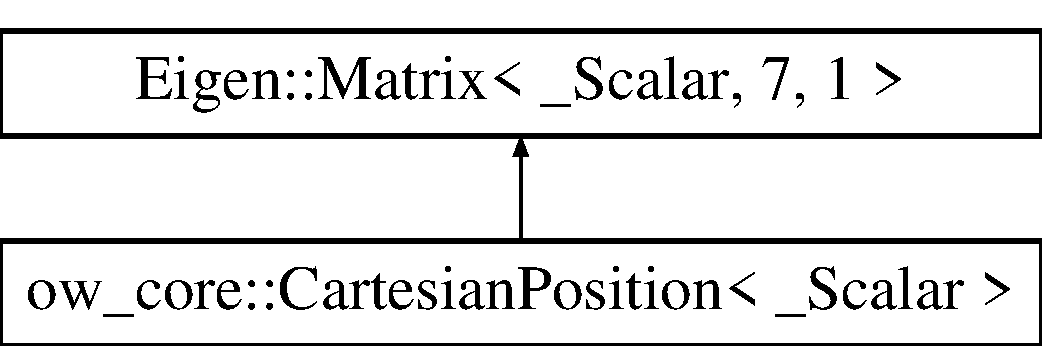
\includegraphics[height=2.000000cm]{d0/d5b/classow__core_1_1CartesianPosition}
\end{center}
\end{figure}
\subsection*{Public Types}
\begin{DoxyCompactItemize}
\item 
typedef \+\_\+\+Scalar {\bfseries Scalar}\hypertarget{classow__core_1_1CartesianPosition_a2d3bae7b8988a5956f61233244a8a038}{}\label{classow__core_1_1CartesianPosition_a2d3bae7b8988a5956f61233244a8a038}

\item 
typedef Eigen\+::\+Matrix$<$ Scalar, 7, 1 $>$ {\bfseries Base}\hypertarget{classow__core_1_1CartesianPosition_a51a56b2c4b9830555602ade3e777fdd8}{}\label{classow__core_1_1CartesianPosition_a51a56b2c4b9830555602ade3e777fdd8}

\item 
typedef Eigen\+::\+Transform$<$ Scalar, 3, Eigen\+::\+Affine $>$ {\bfseries Transform}\hypertarget{classow__core_1_1CartesianPosition_a9c129146a77674691e1c04fe79d142db}{}\label{classow__core_1_1CartesianPosition_a9c129146a77674691e1c04fe79d142db}

\end{DoxyCompactItemize}
\subsection*{Public Member Functions}
\begin{DoxyCompactItemize}
\item 
\hyperlink{classow__core_1_1CartesianPosition_abcb76d25934535197e2c78f66d9389aa}{Cartesian\+Position} ()\hypertarget{classow__core_1_1CartesianPosition_abcb76d25934535197e2c78f66d9389aa}{}\label{classow__core_1_1CartesianPosition_abcb76d25934535197e2c78f66d9389aa}

\begin{DoxyCompactList}\small\item\em Default Constructor. \end{DoxyCompactList}\item 
{\footnotesize template$<$typename Other\+Derived $>$ }\\\hyperlink{classow__core_1_1CartesianPosition_a27da81e6cdf3ffd4f58ee6cdbdb0b7fa}{Cartesian\+Position} (const Eigen\+::\+Eigen\+Base$<$ Other\+Derived $>$ \&other)
\begin{DoxyCompactList}\small\item\em Copy constructor. \end{DoxyCompactList}\item 
\hyperlink{classow__core_1_1CartesianPosition_a87716f0f5fd8a5ddfc1a18fb9205c4fe}{Cartesian\+Position} (const Transform \&other)
\begin{DoxyCompactList}\small\item\em Copy constructor from Eigen\+::\+Transform. \end{DoxyCompactList}\item 
\hyperlink{classow__core_1_1CartesianPosition_adab19102ef4ebb44b39c10842a550ccb}{Cartesian\+Position} (const Scalar \&x, const Scalar \&y, const Scalar \&z, const Scalar \&qw, const Scalar \&qx, const Scalar \&qy, const Scalar \&qz)\hypertarget{classow__core_1_1CartesianPosition_adab19102ef4ebb44b39c10842a550ccb}{}\label{classow__core_1_1CartesianPosition_adab19102ef4ebb44b39c10842a550ccb}

\begin{DoxyCompactList}\small\item\em Constructor from Scalars. \end{DoxyCompactList}\item 
\hyperlink{classow__core_1_1CartesianPosition_a677d43bf7ee688ef2561e3384e0d87af}{Cartesian\+Position} (const typename Transform\+::\+Translation\+Type \&other)
\begin{DoxyCompactList}\small\item\em Copy constructor from Eigen\+::\+Translation. \end{DoxyCompactList}\item 
{\footnotesize template$<$typename Other\+Derived $>$ }\\\hyperlink{classow__core_1_1CartesianPosition_a5facbd98e241518b96c639f645352aff}{Cartesian\+Position} (const Eigen\+::\+Rotation\+Base$<$ Other\+Derived, 3 $>$ \&other)
\begin{DoxyCompactList}\small\item\em Copy constructor from Eigen\+::\+Rotation\+Base. \end{DoxyCompactList}\item 
\hyperlink{classow__core_1_1CartesianPosition_a39f4c6d292b1613e47581e2c5c0584d3}{Cartesian\+Position} (const tf\+::\+Transform \&other)\hypertarget{classow__core_1_1CartesianPosition_a39f4c6d292b1613e47581e2c5c0584d3}{}\label{classow__core_1_1CartesianPosition_a39f4c6d292b1613e47581e2c5c0584d3}

\begin{DoxyCompactList}\small\item\em Copy constructor from tf\+::\+Transform. \end{DoxyCompactList}\item 
\hyperlink{classow__core_1_1CartesianPosition_a12ac7a60828d470c82312a2d9ddcf10a}{Cartesian\+Position} (const geometry\+\_\+msgs\+::\+Pose \&other)\hypertarget{classow__core_1_1CartesianPosition_a12ac7a60828d470c82312a2d9ddcf10a}{}\label{classow__core_1_1CartesianPosition_a12ac7a60828d470c82312a2d9ddcf10a}

\begin{DoxyCompactList}\small\item\em Copy constructor from geometry\+\_\+msgs\+::\+Pose. \end{DoxyCompactList}\item 
void \hyperlink{classow__core_1_1CartesianPosition_a77f179c52a4754479ada9b5ecbdd325a}{set\+Identity} ()\hypertarget{classow__core_1_1CartesianPosition_a77f179c52a4754479ada9b5ecbdd325a}{}\label{classow__core_1_1CartesianPosition_a77f179c52a4754479ada9b5ecbdd325a}

\begin{DoxyCompactList}\small\item\em set to identity. \end{DoxyCompactList}\item 
void \hyperlink{classow__core_1_1CartesianPosition_a94bca79bf37ef9a5ddab1c157bd112ce}{operator=} (const Transform \&T)\hypertarget{classow__core_1_1CartesianPosition_a94bca79bf37ef9a5ddab1c157bd112ce}{}\label{classow__core_1_1CartesianPosition_a94bca79bf37ef9a5ddab1c157bd112ce}

\begin{DoxyCompactList}\small\item\em Assignment form Eigen\+::\+Transformation. \end{DoxyCompactList}\item 
void \hyperlink{classow__core_1_1CartesianPosition_a1384221faaf7c96e225f2cf918e55dab}{operator=} (const tf\+::\+Transform \&T)\hypertarget{classow__core_1_1CartesianPosition_a1384221faaf7c96e225f2cf918e55dab}{}\label{classow__core_1_1CartesianPosition_a1384221faaf7c96e225f2cf918e55dab}

\begin{DoxyCompactList}\small\item\em Assignment form tf\+::\+Transform. \end{DoxyCompactList}\item 
void \hyperlink{classow__core_1_1CartesianPosition_af191c6fbdd039462c5be22192bf2ad33}{operator=} (const geometry\+\_\+msgs\+::\+Pose \&T)\hypertarget{classow__core_1_1CartesianPosition_af191c6fbdd039462c5be22192bf2ad33}{}\label{classow__core_1_1CartesianPosition_af191c6fbdd039462c5be22192bf2ad33}

\begin{DoxyCompactList}\small\item\em Assignment form geometry\+\_\+msgs\+::\+Pose. \end{DoxyCompactList}\item 
{\footnotesize template$<$typename Other\+Derived $>$ }\\void \hyperlink{classow__core_1_1CartesianPosition_affc06373565107ca4fc0df32bf8092c9}{operator=} (const Eigen\+::\+Rotation\+Base$<$ Other\+Derived, 3 $>$ \&R)\hypertarget{classow__core_1_1CartesianPosition_affc06373565107ca4fc0df32bf8092c9}{}\label{classow__core_1_1CartesianPosition_affc06373565107ca4fc0df32bf8092c9}

\begin{DoxyCompactList}\small\item\em Assignment form Eigen\+::\+Rotation\+Base. \end{DoxyCompactList}\item 
void \hyperlink{classow__core_1_1CartesianPosition_ae712894313ad56e5f7aef7cdeff80cc4}{operator=} (const typename Transform\+::\+Translation\+Type \&t)\hypertarget{classow__core_1_1CartesianPosition_ae712894313ad56e5f7aef7cdeff80cc4}{}\label{classow__core_1_1CartesianPosition_ae712894313ad56e5f7aef7cdeff80cc4}

\begin{DoxyCompactList}\small\item\em Assignment form Eigen\+::\+Translation. \end{DoxyCompactList}\item 
\hyperlink{classow__core_1_1CartesianPosition_afbf5dc4ca9164db7474b11c04167f839}{operator Transform} () const \hypertarget{classow__core_1_1CartesianPosition_afbf5dc4ca9164db7474b11c04167f839}{}\label{classow__core_1_1CartesianPosition_afbf5dc4ca9164db7474b11c04167f839}

\begin{DoxyCompactList}\small\item\em Conversion to Eigen\+::\+Transformation. \end{DoxyCompactList}\item 
\hyperlink{classow__core_1_1CartesianPosition_a211d6a1c4da4205d0a5cfbbb1adb88e9}{operator tf\+::\+Transform} () const \hypertarget{classow__core_1_1CartesianPosition_a211d6a1c4da4205d0a5cfbbb1adb88e9}{}\label{classow__core_1_1CartesianPosition_a211d6a1c4da4205d0a5cfbbb1adb88e9}

\begin{DoxyCompactList}\small\item\em Conversion to tf\+::\+Transform. \end{DoxyCompactList}\item 
\hyperlink{classow__core_1_1CartesianPosition_a5911097dc2d04c89baca83fe15f19895}{operator geometry\+\_\+msgs\+::\+Pose} () const \hypertarget{classow__core_1_1CartesianPosition_a5911097dc2d04c89baca83fe15f19895}{}\label{classow__core_1_1CartesianPosition_a5911097dc2d04c89baca83fe15f19895}

\begin{DoxyCompactList}\small\item\em Conversion to geometry\+\_\+msgs\+::\+Pose. \end{DoxyCompactList}\item 
Transform \hyperlink{classow__core_1_1CartesianPosition_a9edd3dd48c3e9167ca5a34e088bd2f20}{to\+Transform\+Eigen} ()\hypertarget{classow__core_1_1CartesianPosition_a9edd3dd48c3e9167ca5a34e088bd2f20}{}\label{classow__core_1_1CartesianPosition_a9edd3dd48c3e9167ca5a34e088bd2f20}

\begin{DoxyCompactList}\small\item\em Conversion to Eigen\+::\+Transformation. \end{DoxyCompactList}\item 
tf\+::\+Transform \hyperlink{classow__core_1_1CartesianPosition_a5511674e38684e3545095c5d1da1a794}{to\+Transform\+Tf} ()\hypertarget{classow__core_1_1CartesianPosition_a5511674e38684e3545095c5d1da1a794}{}\label{classow__core_1_1CartesianPosition_a5511674e38684e3545095c5d1da1a794}

\begin{DoxyCompactList}\small\item\em Conversion to tf\+::\+Transform. \end{DoxyCompactList}\item 
geometry\+\_\+msgs\+::\+Pose \hyperlink{classow__core_1_1CartesianPosition_ace8d8abe4ab2df0f7d9c845b394bcbee}{to\+Pose\+Msg} ()\hypertarget{classow__core_1_1CartesianPosition_ace8d8abe4ab2df0f7d9c845b394bcbee}{}\label{classow__core_1_1CartesianPosition_ace8d8abe4ab2df0f7d9c845b394bcbee}

\begin{DoxyCompactList}\small\item\em Conversion to geometry\+\_\+msgs\+::\+Pose. \end{DoxyCompactList}\item 
\hyperlink{classow__core_1_1LinearPositionRef}{Linear\+Position\+Ref}$<$ Base $>$ \hyperlink{classow__core_1_1CartesianPosition_a88a102e34201fe73051c56a1dc71b9c1}{position} ()\hypertarget{classow__core_1_1CartesianPosition_a88a102e34201fe73051c56a1dc71b9c1}{}\label{classow__core_1_1CartesianPosition_a88a102e34201fe73051c56a1dc71b9c1}

\begin{DoxyCompactList}\small\item\em access to position part \end{DoxyCompactList}\item 
\hyperlink{classow__core_1_1LinearPositionRef}{Linear\+Position\+Ref}$<$ const Base $>$ \hyperlink{classow__core_1_1CartesianPosition_adcb4a6deef06f26423e7a6ce5943d83e}{position} () const \hypertarget{classow__core_1_1CartesianPosition_adcb4a6deef06f26423e7a6ce5943d83e}{}\label{classow__core_1_1CartesianPosition_adcb4a6deef06f26423e7a6ce5943d83e}

\begin{DoxyCompactList}\small\item\em const access to position part \end{DoxyCompactList}\item 
\hyperlink{classow__core_1_1AngularPositionRef}{Angular\+Position\+Ref}$<$ Base $>$ \hyperlink{classow__core_1_1CartesianPosition_a1e7078e6698fcefe907e45d82df18fab}{orientation} ()\hypertarget{classow__core_1_1CartesianPosition_a1e7078e6698fcefe907e45d82df18fab}{}\label{classow__core_1_1CartesianPosition_a1e7078e6698fcefe907e45d82df18fab}

\begin{DoxyCompactList}\small\item\em access to orientation part \end{DoxyCompactList}\item 
\hyperlink{classow__core_1_1AngularPositionRef}{Angular\+Position\+Ref}$<$ const Base $>$ \hyperlink{classow__core_1_1CartesianPosition_aebff574a5f054528f777f1151e9f0798}{orientation} () const \hypertarget{classow__core_1_1CartesianPosition_aebff574a5f054528f777f1151e9f0798}{}\label{classow__core_1_1CartesianPosition_aebff574a5f054528f777f1151e9f0798}

\begin{DoxyCompactList}\small\item\em const access to orientation part \end{DoxyCompactList}\item 
std\+::string \hyperlink{classow__core_1_1CartesianPosition_adb579e0cf4b5dc64a276e5850fdf7d92}{to\+String} () const \hypertarget{classow__core_1_1CartesianPosition_adb579e0cf4b5dc64a276e5850fdf7d92}{}\label{classow__core_1_1CartesianPosition_adb579e0cf4b5dc64a276e5850fdf7d92}

\begin{DoxyCompactList}\small\item\em Conversion to std\+::string. \end{DoxyCompactList}\end{DoxyCompactItemize}
\subsection*{Static Public Member Functions}
\begin{DoxyCompactItemize}
\item 
static const \hyperlink{classow__core_1_1CartesianPosition}{Cartesian\+Position} \& \hyperlink{classow__core_1_1CartesianPosition_adf7c4725b0e7c01554d431f1277b7380}{Identity} ()
\begin{DoxyCompactList}\small\item\em Construct as Identity. \end{DoxyCompactList}\item 
static const \hyperlink{classow__core_1_1CartesianPosition}{Cartesian\+Position} \& \hyperlink{classow__core_1_1CartesianPosition_acd8dec83eb36d0042810e9917f9ab52f}{Default} ()
\begin{DoxyCompactList}\small\item\em Construct as Default. \end{DoxyCompactList}\end{DoxyCompactItemize}


\subsection{Detailed Description}
\subsubsection*{template$<$typename \+\_\+\+Scalar$>$\\*
class ow\+\_\+core\+::\+Cartesian\+Position$<$ \+\_\+\+Scalar $>$}

The \hyperlink{classow__core_1_1CartesianPosition}{Cartesian\+Position} class. 

The \hyperlink{classow__core_1_1CartesianPosition}{Cartesian\+Position} is of type Eigen\+::\+Vector7 and is represented by the math symbol $\mathbf{X}$.

Stores the position and orientation information in a 7 dimensional vector. The position part is represented by the first three elements. The orientation as a quaternion by the last four elements. 

\subsection{Constructor \& Destructor Documentation}
\index{ow\+\_\+core\+::\+Cartesian\+Position@{ow\+\_\+core\+::\+Cartesian\+Position}!Cartesian\+Position@{Cartesian\+Position}}
\index{Cartesian\+Position@{Cartesian\+Position}!ow\+\_\+core\+::\+Cartesian\+Position@{ow\+\_\+core\+::\+Cartesian\+Position}}
\subsubsection[{\texorpdfstring{Cartesian\+Position(const Eigen\+::\+Eigen\+Base$<$ Other\+Derived $>$ \&other)}{CartesianPosition(const Eigen::EigenBase< OtherDerived > &other)}}]{\setlength{\rightskip}{0pt plus 5cm}template$<$typename \+\_\+\+Scalar $>$ template$<$typename Other\+Derived $>$ {\bf ow\+\_\+core\+::\+Cartesian\+Position}$<$ \+\_\+\+Scalar $>$\+::{\bf Cartesian\+Position} (
\begin{DoxyParamCaption}
\item[{const Eigen\+::\+Eigen\+Base$<$ Other\+Derived $>$ \&}]{other}
\end{DoxyParamCaption}
)\hspace{0.3cm}{\ttfamily [inline]}}\hypertarget{classow__core_1_1CartesianPosition_a27da81e6cdf3ffd4f58ee6cdbdb0b7fa}{}\label{classow__core_1_1CartesianPosition_a27da81e6cdf3ffd4f58ee6cdbdb0b7fa}


Copy constructor. 

This copy constructor not only works with Eigen matrices but also with their expressions. \index{ow\+\_\+core\+::\+Cartesian\+Position@{ow\+\_\+core\+::\+Cartesian\+Position}!Cartesian\+Position@{Cartesian\+Position}}
\index{Cartesian\+Position@{Cartesian\+Position}!ow\+\_\+core\+::\+Cartesian\+Position@{ow\+\_\+core\+::\+Cartesian\+Position}}
\subsubsection[{\texorpdfstring{Cartesian\+Position(const Transform \&other)}{CartesianPosition(const Transform &other)}}]{\setlength{\rightskip}{0pt plus 5cm}template$<$typename \+\_\+\+Scalar $>$ {\bf ow\+\_\+core\+::\+Cartesian\+Position}$<$ \+\_\+\+Scalar $>$\+::{\bf Cartesian\+Position} (
\begin{DoxyParamCaption}
\item[{const Transform \&}]{other}
\end{DoxyParamCaption}
)\hspace{0.3cm}{\ttfamily [inline]}}\hypertarget{classow__core_1_1CartesianPosition_a87716f0f5fd8a5ddfc1a18fb9205c4fe}{}\label{classow__core_1_1CartesianPosition_a87716f0f5fd8a5ddfc1a18fb9205c4fe}


Copy constructor from Eigen\+::\+Transform. 

\begin{DoxyRefDesc}{Todo}
\item[\hyperlink{todo__todo000003}{Todo}]\+: removed explicit to write things like\+: \hyperlink{classow__core_1_1CartesianPosition}{Cartesian\+Position} X = Eigen\+::\+Affine3d\+::\+Identity(); \end{DoxyRefDesc}
\index{ow\+\_\+core\+::\+Cartesian\+Position@{ow\+\_\+core\+::\+Cartesian\+Position}!Cartesian\+Position@{Cartesian\+Position}}
\index{Cartesian\+Position@{Cartesian\+Position}!ow\+\_\+core\+::\+Cartesian\+Position@{ow\+\_\+core\+::\+Cartesian\+Position}}
\subsubsection[{\texorpdfstring{Cartesian\+Position(const typename Transform\+::\+Translation\+Type \&other)}{CartesianPosition(const typename Transform::TranslationType &other)}}]{\setlength{\rightskip}{0pt plus 5cm}template$<$typename \+\_\+\+Scalar $>$ {\bf ow\+\_\+core\+::\+Cartesian\+Position}$<$ \+\_\+\+Scalar $>$\+::{\bf Cartesian\+Position} (
\begin{DoxyParamCaption}
\item[{const typename Transform\+::\+Translation\+Type \&}]{other}
\end{DoxyParamCaption}
)\hspace{0.3cm}{\ttfamily [inline]}, {\ttfamily [explicit]}}\hypertarget{classow__core_1_1CartesianPosition_a677d43bf7ee688ef2561e3384e0d87af}{}\label{classow__core_1_1CartesianPosition_a677d43bf7ee688ef2561e3384e0d87af}


Copy constructor from Eigen\+::\+Translation. 

This Constructor sets the rotational part to identity. \index{ow\+\_\+core\+::\+Cartesian\+Position@{ow\+\_\+core\+::\+Cartesian\+Position}!Cartesian\+Position@{Cartesian\+Position}}
\index{Cartesian\+Position@{Cartesian\+Position}!ow\+\_\+core\+::\+Cartesian\+Position@{ow\+\_\+core\+::\+Cartesian\+Position}}
\subsubsection[{\texorpdfstring{Cartesian\+Position(const Eigen\+::\+Rotation\+Base$<$ Other\+Derived, 3 $>$ \&other)}{CartesianPosition(const Eigen::RotationBase< OtherDerived, 3 > &other)}}]{\setlength{\rightskip}{0pt plus 5cm}template$<$typename \+\_\+\+Scalar $>$ template$<$typename Other\+Derived $>$ {\bf ow\+\_\+core\+::\+Cartesian\+Position}$<$ \+\_\+\+Scalar $>$\+::{\bf Cartesian\+Position} (
\begin{DoxyParamCaption}
\item[{const Eigen\+::\+Rotation\+Base$<$ Other\+Derived, 3 $>$ \&}]{other}
\end{DoxyParamCaption}
)\hspace{0.3cm}{\ttfamily [inline]}, {\ttfamily [explicit]}}\hypertarget{classow__core_1_1CartesianPosition_a5facbd98e241518b96c639f645352aff}{}\label{classow__core_1_1CartesianPosition_a5facbd98e241518b96c639f645352aff}


Copy constructor from Eigen\+::\+Rotation\+Base. 

This Constructor sets the translational part to zero. 

\subsection{Member Function Documentation}
\index{ow\+\_\+core\+::\+Cartesian\+Position@{ow\+\_\+core\+::\+Cartesian\+Position}!Default@{Default}}
\index{Default@{Default}!ow\+\_\+core\+::\+Cartesian\+Position@{ow\+\_\+core\+::\+Cartesian\+Position}}
\subsubsection[{\texorpdfstring{Default()}{Default()}}]{\setlength{\rightskip}{0pt plus 5cm}template$<$typename \+\_\+\+Scalar $>$ static const {\bf Cartesian\+Position}\& {\bf ow\+\_\+core\+::\+Cartesian\+Position}$<$ \+\_\+\+Scalar $>$\+::Default (
\begin{DoxyParamCaption}
{}
\end{DoxyParamCaption}
)\hspace{0.3cm}{\ttfamily [inline]}, {\ttfamily [static]}}\hypertarget{classow__core_1_1CartesianPosition_acd8dec83eb36d0042810e9917f9ab52f}{}\label{classow__core_1_1CartesianPosition_acd8dec83eb36d0042810e9917f9ab52f}


Construct as Default. 

Default is Identity \index{ow\+\_\+core\+::\+Cartesian\+Position@{ow\+\_\+core\+::\+Cartesian\+Position}!Identity@{Identity}}
\index{Identity@{Identity}!ow\+\_\+core\+::\+Cartesian\+Position@{ow\+\_\+core\+::\+Cartesian\+Position}}
\subsubsection[{\texorpdfstring{Identity()}{Identity()}}]{\setlength{\rightskip}{0pt plus 5cm}template$<$typename \+\_\+\+Scalar $>$ static const {\bf Cartesian\+Position}\& {\bf ow\+\_\+core\+::\+Cartesian\+Position}$<$ \+\_\+\+Scalar $>$\+::Identity (
\begin{DoxyParamCaption}
{}
\end{DoxyParamCaption}
)\hspace{0.3cm}{\ttfamily [inline]}, {\ttfamily [static]}}\hypertarget{classow__core_1_1CartesianPosition_adf7c4725b0e7c01554d431f1277b7380}{}\label{classow__core_1_1CartesianPosition_adf7c4725b0e7c01554d431f1277b7380}


Construct as Identity. 

\begin{DoxyRefDesc}{Todo}
\item[\hyperlink{todo__todo000002}{Todo}]maby expression \end{DoxyRefDesc}


The documentation for this class was generated from the following file\+:\begin{DoxyCompactItemize}
\item 
/home/dean/ros/workspaces/ow\+\_\+test\+\_\+ws/src/ow\+\_\+core/include/ow\+\_\+core/\hyperlink{cartesian__position_8h}{cartesian\+\_\+position.\+h}\end{DoxyCompactItemize}

\hypertarget{classow__core_1_1CartesianVelocity}{}\section{ow\+\_\+core\+:\+:Cartesian\+Velocity$<$ \+\_\+\+Scalar $>$ Class Template Reference}
\label{classow__core_1_1CartesianVelocity}\index{ow\+\_\+core\+::\+Cartesian\+Velocity$<$ \+\_\+\+Scalar $>$@{ow\+\_\+core\+::\+Cartesian\+Velocity$<$ \+\_\+\+Scalar $>$}}


The \hyperlink{classow__core_1_1CartesianVelocity}{Cartesian\+Velocity} class.  




{\ttfamily \#include $<$cartesian\+\_\+velocity.\+h$>$}

Inheritance diagram for ow\+\_\+core\+:\+:Cartesian\+Velocity$<$ \+\_\+\+Scalar $>$\+:\begin{figure}[H]
\begin{center}
\leavevmode
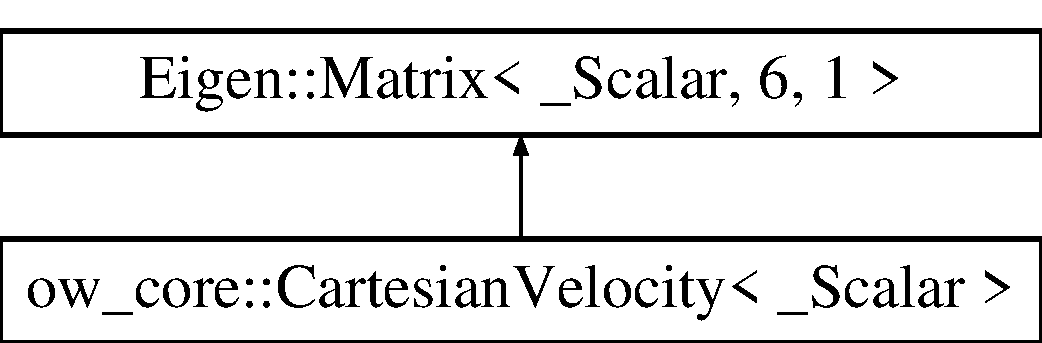
\includegraphics[height=2.000000cm]{d5/df0/classow__core_1_1CartesianVelocity}
\end{center}
\end{figure}
\subsection*{Public Types}
\begin{DoxyCompactItemize}
\item 
typedef \+\_\+\+Scalar {\bfseries Scalar}\hypertarget{classow__core_1_1CartesianVelocity_a30fbc2ff4d9a2902e22c1013d5c79adf}{}\label{classow__core_1_1CartesianVelocity_a30fbc2ff4d9a2902e22c1013d5c79adf}

\item 
typedef Eigen\+::\+Matrix$<$ Scalar, 6, 1 $>$ {\bfseries Base}\hypertarget{classow__core_1_1CartesianVelocity_afb19f3c2efe2446b76a716a0809e960f}{}\label{classow__core_1_1CartesianVelocity_afb19f3c2efe2446b76a716a0809e960f}

\end{DoxyCompactItemize}
\subsection*{Public Member Functions}
\begin{DoxyCompactItemize}
\item 
\hyperlink{classow__core_1_1CartesianVelocity_a9101c643b5b96005b9fa87439c6bf805}{Cartesian\+Velocity} ()\hypertarget{classow__core_1_1CartesianVelocity_a9101c643b5b96005b9fa87439c6bf805}{}\label{classow__core_1_1CartesianVelocity_a9101c643b5b96005b9fa87439c6bf805}

\begin{DoxyCompactList}\small\item\em Default Constructor. \end{DoxyCompactList}\item 
{\footnotesize template$<$typename Other\+Derived $>$ }\\\hyperlink{classow__core_1_1CartesianVelocity_a3b2f280aae9e691e428c6317aa608d61}{Cartesian\+Velocity} (const Eigen\+::\+Eigen\+Base$<$ Other\+Derived $>$ \&other)
\begin{DoxyCompactList}\small\item\em Copy constructor. \end{DoxyCompactList}\item 
\hyperlink{classow__core_1_1CartesianVelocity_a941e816cd2c1aacaef90fa02f75b2433}{Cartesian\+Velocity} (const geometry\+\_\+msgs\+::\+Twist \&other)\hypertarget{classow__core_1_1CartesianVelocity_a941e816cd2c1aacaef90fa02f75b2433}{}\label{classow__core_1_1CartesianVelocity_a941e816cd2c1aacaef90fa02f75b2433}

\begin{DoxyCompactList}\small\item\em Copy constructor form geometry\+\_\+msgs\+::\+Twist. \end{DoxyCompactList}\item 
void \hyperlink{classow__core_1_1CartesianVelocity_ac4abf76a3ffb12d811c7ede84aeb0281}{operator=} (const geometry\+\_\+msgs\+::\+Twist \&Xp)\hypertarget{classow__core_1_1CartesianVelocity_ac4abf76a3ffb12d811c7ede84aeb0281}{}\label{classow__core_1_1CartesianVelocity_ac4abf76a3ffb12d811c7ede84aeb0281}

\begin{DoxyCompactList}\small\item\em Assignment form geometry\+\_\+msgs\+::\+Twist. \end{DoxyCompactList}\item 
\hyperlink{classow__core_1_1CartesianVelocity_ad3566f959c904cf22a4f1228290f8c15}{operator geometry\+\_\+msgs\+::\+Twist} () const \hypertarget{classow__core_1_1CartesianVelocity_ad3566f959c904cf22a4f1228290f8c15}{}\label{classow__core_1_1CartesianVelocity_ad3566f959c904cf22a4f1228290f8c15}

\begin{DoxyCompactList}\small\item\em Conversion to geometry\+\_\+msgs\+::\+Twist. \end{DoxyCompactList}\item 
geometry\+\_\+msgs\+::\+Twist \hyperlink{classow__core_1_1CartesianVelocity_a554aac9c93626cd576444a4fead7ac7f}{to\+Twist\+Msg} () const \hypertarget{classow__core_1_1CartesianVelocity_a554aac9c93626cd576444a4fead7ac7f}{}\label{classow__core_1_1CartesianVelocity_a554aac9c93626cd576444a4fead7ac7f}

\begin{DoxyCompactList}\small\item\em Conversion to geometry\+\_\+msgs\+::\+Twist. \end{DoxyCompactList}\item 
\hyperlink{classow__core_1_1LinearVelocityRef}{Linear\+Velocity\+Ref}$<$ Base $>$ \hyperlink{classow__core_1_1CartesianVelocity_acdd527df069a117b5395e0e667b5a267}{linear} ()\hypertarget{classow__core_1_1CartesianVelocity_acdd527df069a117b5395e0e667b5a267}{}\label{classow__core_1_1CartesianVelocity_acdd527df069a117b5395e0e667b5a267}

\begin{DoxyCompactList}\small\item\em access to linear part \end{DoxyCompactList}\item 
\hyperlink{classow__core_1_1LinearVelocityRef}{Linear\+Velocity\+Ref}$<$ const Base $>$ \hyperlink{classow__core_1_1CartesianVelocity_a06fd2a41cffc8c2b469254befd4d5e18}{linear} () const \hypertarget{classow__core_1_1CartesianVelocity_a06fd2a41cffc8c2b469254befd4d5e18}{}\label{classow__core_1_1CartesianVelocity_a06fd2a41cffc8c2b469254befd4d5e18}

\begin{DoxyCompactList}\small\item\em const access to linear part \end{DoxyCompactList}\item 
\hyperlink{classow__core_1_1AngularVelocityRef}{Angular\+Velocity\+Ref}$<$ Base $>$ \hyperlink{classow__core_1_1CartesianVelocity_adc8e89cb3eeb678bc74061c696bbd30d}{angular} ()\hypertarget{classow__core_1_1CartesianVelocity_adc8e89cb3eeb678bc74061c696bbd30d}{}\label{classow__core_1_1CartesianVelocity_adc8e89cb3eeb678bc74061c696bbd30d}

\begin{DoxyCompactList}\small\item\em access to angular part \end{DoxyCompactList}\item 
\hyperlink{classow__core_1_1AngularVelocityRef}{Angular\+Velocity\+Ref}$<$ const Base $>$ \hyperlink{classow__core_1_1CartesianVelocity_ab16fa37cdaada03fcb94ef0b2cd008aa}{angular} () const \hypertarget{classow__core_1_1CartesianVelocity_ab16fa37cdaada03fcb94ef0b2cd008aa}{}\label{classow__core_1_1CartesianVelocity_ab16fa37cdaada03fcb94ef0b2cd008aa}

\begin{DoxyCompactList}\small\item\em const access to angular part \end{DoxyCompactList}\item 
std\+::string \hyperlink{classow__core_1_1CartesianVelocity_ae78d83f858be0085a2d564a84aa32722}{to\+String} () const \hypertarget{classow__core_1_1CartesianVelocity_ae78d83f858be0085a2d564a84aa32722}{}\label{classow__core_1_1CartesianVelocity_ae78d83f858be0085a2d564a84aa32722}

\begin{DoxyCompactList}\small\item\em Conversion to std\+::string. \end{DoxyCompactList}\end{DoxyCompactItemize}
\subsection*{Static Public Member Functions}
\begin{DoxyCompactItemize}
\item 
static const \hyperlink{classow__core_1_1CartesianVelocity}{Cartesian\+Velocity}$<$ Scalar $>$ \& \hyperlink{classow__core_1_1CartesianVelocity_ab9823aafa0100aa054396668a32324c1}{Default} ()
\begin{DoxyCompactList}\small\item\em Construct as Default. \end{DoxyCompactList}\end{DoxyCompactItemize}


\subsection{Detailed Description}
\subsubsection*{template$<$typename \+\_\+\+Scalar$>$\\*
class ow\+\_\+core\+::\+Cartesian\+Velocity$<$ \+\_\+\+Scalar $>$}

The \hyperlink{classow__core_1_1CartesianVelocity}{Cartesian\+Velocity} class. 

The \hyperlink{classow__core_1_1CartesianVelocity}{Cartesian\+Velocity} is of type Eigen\+::\+Vector6 and is represented by the math symbol $\dot{\mathbf{X}}$.

Stores the linear and angular velocity in a 6 dimensional vector. The linear velocity part is represented by the first three elements. The angular velocity by the last three elements. 

\subsection{Constructor \& Destructor Documentation}
\index{ow\+\_\+core\+::\+Cartesian\+Velocity@{ow\+\_\+core\+::\+Cartesian\+Velocity}!Cartesian\+Velocity@{Cartesian\+Velocity}}
\index{Cartesian\+Velocity@{Cartesian\+Velocity}!ow\+\_\+core\+::\+Cartesian\+Velocity@{ow\+\_\+core\+::\+Cartesian\+Velocity}}
\subsubsection[{\texorpdfstring{Cartesian\+Velocity(const Eigen\+::\+Eigen\+Base$<$ Other\+Derived $>$ \&other)}{CartesianVelocity(const Eigen::EigenBase< OtherDerived > &other)}}]{\setlength{\rightskip}{0pt plus 5cm}template$<$typename \+\_\+\+Scalar $>$ template$<$typename Other\+Derived $>$ {\bf ow\+\_\+core\+::\+Cartesian\+Velocity}$<$ \+\_\+\+Scalar $>$\+::{\bf Cartesian\+Velocity} (
\begin{DoxyParamCaption}
\item[{const Eigen\+::\+Eigen\+Base$<$ Other\+Derived $>$ \&}]{other}
\end{DoxyParamCaption}
)\hspace{0.3cm}{\ttfamily [inline]}}\hypertarget{classow__core_1_1CartesianVelocity_a3b2f280aae9e691e428c6317aa608d61}{}\label{classow__core_1_1CartesianVelocity_a3b2f280aae9e691e428c6317aa608d61}


Copy constructor. 

This copy constructor not only works with Eigen matrices but also with their expressions. 

\subsection{Member Function Documentation}
\index{ow\+\_\+core\+::\+Cartesian\+Velocity@{ow\+\_\+core\+::\+Cartesian\+Velocity}!Default@{Default}}
\index{Default@{Default}!ow\+\_\+core\+::\+Cartesian\+Velocity@{ow\+\_\+core\+::\+Cartesian\+Velocity}}
\subsubsection[{\texorpdfstring{Default()}{Default()}}]{\setlength{\rightskip}{0pt plus 5cm}template$<$typename \+\_\+\+Scalar $>$ static const {\bf Cartesian\+Velocity}$<$Scalar$>$\& {\bf ow\+\_\+core\+::\+Cartesian\+Velocity}$<$ \+\_\+\+Scalar $>$\+::Default (
\begin{DoxyParamCaption}
{}
\end{DoxyParamCaption}
)\hspace{0.3cm}{\ttfamily [inline]}, {\ttfamily [static]}}\hypertarget{classow__core_1_1CartesianVelocity_ab9823aafa0100aa054396668a32324c1}{}\label{classow__core_1_1CartesianVelocity_ab9823aafa0100aa054396668a32324c1}


Construct as Default. 

Default is Identity 

The documentation for this class was generated from the following file\+:\begin{DoxyCompactItemize}
\item 
/home/dean/ros/workspaces/ow\+\_\+test\+\_\+ws/src/ow\+\_\+core/include/ow\+\_\+core/\hyperlink{cartesian__velocity_8h}{cartesian\+\_\+velocity.\+h}\end{DoxyCompactItemize}

\hypertarget{classow__plugin__loader_1_1ClassCreator}{}\section{ow\+\_\+plugin\+\_\+loader\+:\+:Class\+Creator Class Reference}
\label{classow__plugin__loader_1_1ClassCreator}\index{ow\+\_\+plugin\+\_\+loader\+::\+Class\+Creator@{ow\+\_\+plugin\+\_\+loader\+::\+Class\+Creator}}


The \hyperlink{classow__plugin__loader_1_1ClassCreator}{Class\+Creator} class.  




{\ttfamily \#include $<$class\+\_\+creator.\+h$>$}

\subsection*{Public Types}
\begin{DoxyCompactItemize}
\item 
typedef \hyperlink{classow__core_1_1IGenericClass}{ow\+\_\+core\+::\+I\+Generic\+Class} {\bfseries I\+Generic\+Class}\hypertarget{classow__plugin__loader_1_1ClassCreator_ac2324a34c491c3e3edf855ff06453531}{}\label{classow__plugin__loader_1_1ClassCreator_ac2324a34c491c3e3edf855ff06453531}

\end{DoxyCompactItemize}
\subsection*{Public Member Functions}
\begin{DoxyCompactItemize}
\item 
\hyperlink{classow__plugin__loader_1_1ClassCreator_aa18171c6438da1053868549a99d798fd}{Class\+Creator} (const std\+::string \&lib\+File\+Path, bool $\ast$ok=0)
\begin{DoxyCompactList}\small\item\em Default constructor. \end{DoxyCompactList}\item 
virtual \hyperlink{classow__plugin__loader_1_1ClassCreator_a0020c21b86a1acaf0824a07139e6ef82}{$\sim$\+Class\+Creator} ()\hypertarget{classow__plugin__loader_1_1ClassCreator_a0020c21b86a1acaf0824a07139e6ef82}{}\label{classow__plugin__loader_1_1ClassCreator_a0020c21b86a1acaf0824a07139e6ef82}

\begin{DoxyCompactList}\small\item\em Deconstructor. \end{DoxyCompactList}\item 
\hyperlink{classow__core_1_1IGenericClass}{I\+Generic\+Class} $\ast$ \hyperlink{classow__plugin__loader_1_1ClassCreator_a69208f3b46de111a3a3820a8c2bb726a}{generic\+Class\+Ptr} ()
\begin{DoxyCompactList}\small\item\em Generic pointer to the created class. \end{DoxyCompactList}\item 
{\footnotesize template$<$class I\+Class $>$ }\\I\+Class $\ast$ \hyperlink{classow__plugin__loader_1_1ClassCreator_a135ab5f75eb0d1538d02eee8c3f1278e}{class\+Ptr} ()
\begin{DoxyCompactList}\small\item\em Interface class pointer to the created class. \end{DoxyCompactList}\end{DoxyCompactItemize}
\subsection*{Protected Attributes}
\begin{DoxyCompactItemize}
\item 
\hyperlink{classow__plugin__loader_1_1ClassLoader}{Class\+Loader} \hyperlink{classow__plugin__loader_1_1ClassCreator_aded4b5806eac1add44b05a92f60d3596}{loader\+\_\+}\hypertarget{classow__plugin__loader_1_1ClassCreator_aded4b5806eac1add44b05a92f60d3596}{}\label{classow__plugin__loader_1_1ClassCreator_aded4b5806eac1add44b05a92f60d3596}

\begin{DoxyCompactList}\small\item\em class loader \end{DoxyCompactList}\item 
\hyperlink{classow__core_1_1IGenericClass}{I\+Generic\+Class} $\ast$ \hyperlink{classow__plugin__loader_1_1ClassCreator_a4bf4cda4e02e535f9d7e675a31241187}{c\+\_\+ptr\+\_\+}\hypertarget{classow__plugin__loader_1_1ClassCreator_a4bf4cda4e02e535f9d7e675a31241187}{}\label{classow__plugin__loader_1_1ClassCreator_a4bf4cda4e02e535f9d7e675a31241187}

\begin{DoxyCompactList}\small\item\em the pointer to the created class \end{DoxyCompactList}\end{DoxyCompactItemize}


\subsection{Detailed Description}
The \hyperlink{classow__plugin__loader_1_1ClassCreator}{Class\+Creator} class. 

This class can load shared libs at runtime and can create classes from the loaded lib. In contrast to the class loader, this class creates only one instance of the loaded class and manages its pointer. 

\subsection{Constructor \& Destructor Documentation}
\index{ow\+\_\+plugin\+\_\+loader\+::\+Class\+Creator@{ow\+\_\+plugin\+\_\+loader\+::\+Class\+Creator}!Class\+Creator@{Class\+Creator}}
\index{Class\+Creator@{Class\+Creator}!ow\+\_\+plugin\+\_\+loader\+::\+Class\+Creator@{ow\+\_\+plugin\+\_\+loader\+::\+Class\+Creator}}
\subsubsection[{\texorpdfstring{Class\+Creator(const std\+::string \&lib\+File\+Path, bool $\ast$ok=0)}{ClassCreator(const std::string &libFilePath, bool *ok=0)}}]{\setlength{\rightskip}{0pt plus 5cm}ow\+\_\+plugin\+\_\+loader\+::\+Class\+Creator\+::\+Class\+Creator (
\begin{DoxyParamCaption}
\item[{const std\+::string \&}]{lib\+File\+Path, }
\item[{bool $\ast$}]{ok = {\ttfamily 0}}
\end{DoxyParamCaption}
)}\hypertarget{classow__plugin__loader_1_1ClassCreator_aa18171c6438da1053868549a99d798fd}{}\label{classow__plugin__loader_1_1ClassCreator_aa18171c6438da1053868549a99d798fd}


Default constructor. 


\begin{DoxyParams}{Parameters}
{\em lib\+File\+Path} & the file path to the .so shared library to use.\\
\hline
{\em ok} & optional flag that is set to true on success or set to false on error. \\
\hline
\end{DoxyParams}


\subsection{Member Function Documentation}
\index{ow\+\_\+plugin\+\_\+loader\+::\+Class\+Creator@{ow\+\_\+plugin\+\_\+loader\+::\+Class\+Creator}!class\+Ptr@{class\+Ptr}}
\index{class\+Ptr@{class\+Ptr}!ow\+\_\+plugin\+\_\+loader\+::\+Class\+Creator@{ow\+\_\+plugin\+\_\+loader\+::\+Class\+Creator}}
\subsubsection[{\texorpdfstring{class\+Ptr()}{classPtr()}}]{\setlength{\rightskip}{0pt plus 5cm}template$<$class I\+Class $>$ I\+Class$\ast$ ow\+\_\+plugin\+\_\+loader\+::\+Class\+Creator\+::class\+Ptr (
\begin{DoxyParamCaption}
{}
\end{DoxyParamCaption}
)\hspace{0.3cm}{\ttfamily [inline]}}\hypertarget{classow__plugin__loader_1_1ClassCreator_a135ab5f75eb0d1538d02eee8c3f1278e}{}\label{classow__plugin__loader_1_1ClassCreator_a135ab5f75eb0d1538d02eee8c3f1278e}


Interface class pointer to the created class. 

This pointer is 0 on error.

N\+O\+TE\+: the creation and deletion of the created class is managed by this class. You should not delete the class to which this pointer is pointing. \index{ow\+\_\+plugin\+\_\+loader\+::\+Class\+Creator@{ow\+\_\+plugin\+\_\+loader\+::\+Class\+Creator}!generic\+Class\+Ptr@{generic\+Class\+Ptr}}
\index{generic\+Class\+Ptr@{generic\+Class\+Ptr}!ow\+\_\+plugin\+\_\+loader\+::\+Class\+Creator@{ow\+\_\+plugin\+\_\+loader\+::\+Class\+Creator}}
\subsubsection[{\texorpdfstring{generic\+Class\+Ptr()}{genericClassPtr()}}]{\setlength{\rightskip}{0pt plus 5cm}{\bf I\+Generic\+Class}$\ast$ ow\+\_\+plugin\+\_\+loader\+::\+Class\+Creator\+::generic\+Class\+Ptr (
\begin{DoxyParamCaption}
{}
\end{DoxyParamCaption}
)}\hypertarget{classow__plugin__loader_1_1ClassCreator_a69208f3b46de111a3a3820a8c2bb726a}{}\label{classow__plugin__loader_1_1ClassCreator_a69208f3b46de111a3a3820a8c2bb726a}


Generic pointer to the created class. 

This pointer is 0 on error.

N\+O\+TE\+: the creation and deletion of the created class is managed by this class. You should not delete the class to which this pointer is pointing. 

The documentation for this class was generated from the following file\+:\begin{DoxyCompactItemize}
\item 
/home/dean/ros/workspaces/ow\+\_\+test\+\_\+ws/src/ow\+\_\+plugin\+\_\+loader/include/ow\+\_\+plugin\+\_\+loader/\hyperlink{class__creator_8h}{class\+\_\+creator.\+h}\end{DoxyCompactItemize}

\hypertarget{classow__plugin__loader_1_1ClassLoader}{}\section{ow\+\_\+plugin\+\_\+loader\+:\+:Class\+Loader Class Reference}
\label{classow__plugin__loader_1_1ClassLoader}\index{ow\+\_\+plugin\+\_\+loader\+::\+Class\+Loader@{ow\+\_\+plugin\+\_\+loader\+::\+Class\+Loader}}


The \hyperlink{classow__plugin__loader_1_1ClassLoader}{Class\+Loader} class.  




{\ttfamily \#include $<$class\+\_\+loader.\+h$>$}

\subsection*{Public Types}
\begin{DoxyCompactItemize}
\item 
typedef \hyperlink{classow__core_1_1IGenericClass}{ow\+\_\+core\+::\+I\+Generic\+Class} {\bfseries I\+Generic\+Class}\hypertarget{classow__plugin__loader_1_1ClassLoader_aeb268b387f1810a002e0927e2f72a9d5}{}\label{classow__plugin__loader_1_1ClassLoader_aeb268b387f1810a002e0927e2f72a9d5}

\end{DoxyCompactItemize}
\subsection*{Public Member Functions}
\begin{DoxyCompactItemize}
\item 
\hyperlink{classow__plugin__loader_1_1ClassLoader_a6578b700790fbf7659e81aceabee7630}{Class\+Loader} (const std\+::string \&lib\+File\+Path=\char`\"{}\char`\"{})\hypertarget{classow__plugin__loader_1_1ClassLoader_a6578b700790fbf7659e81aceabee7630}{}\label{classow__plugin__loader_1_1ClassLoader_a6578b700790fbf7659e81aceabee7630}

\begin{DoxyCompactList}\small\item\em Default constructor. \end{DoxyCompactList}\item 
virtual \hyperlink{classow__plugin__loader_1_1ClassLoader_a8c85ba871c8a9caf9734eaf5111bee63}{$\sim$\+Class\+Loader} ()\hypertarget{classow__plugin__loader_1_1ClassLoader_a8c85ba871c8a9caf9734eaf5111bee63}{}\label{classow__plugin__loader_1_1ClassLoader_a8c85ba871c8a9caf9734eaf5111bee63}

\begin{DoxyCompactList}\small\item\em Deconstructor. \end{DoxyCompactList}\item 
bool \hyperlink{classow__plugin__loader_1_1ClassLoader_aa748690ab43967584daff8db4269fa49}{open} (const std\+::string \&lib\+File\+Path=\char`\"{}\char`\"{})
\begin{DoxyCompactList}\small\item\em Open and load the shared lib which contains the desired class to create. \end{DoxyCompactList}\item 
bool \hyperlink{classow__plugin__loader_1_1ClassLoader_ae1b7d5da12b27e6ffbf34b9b8242e4f1}{close} ()
\begin{DoxyCompactList}\small\item\em Unload and close the shared lib. \end{DoxyCompactList}\item 
bool {\bfseries is\+Opened} () const \hypertarget{classow__plugin__loader_1_1ClassLoader_a6fc48740bceb814da7af5ccdfe5ec6bb}{}\label{classow__plugin__loader_1_1ClassLoader_a6fc48740bceb814da7af5ccdfe5ec6bb}

\item 
bool {\bfseries is\+Closed} () const \hypertarget{classow__plugin__loader_1_1ClassLoader_a32af91737fb08d8d40007ed9e8ad7acb}{}\label{classow__plugin__loader_1_1ClassLoader_a32af91737fb08d8d40007ed9e8ad7acb}

\item 
\hyperlink{classow__core_1_1IGenericClass}{I\+Generic\+Class} $\ast$ \hyperlink{classow__plugin__loader_1_1ClassLoader_a6091dfbec7f40133d6308c8944f593e4}{create\+Class\+Generic} ()\hypertarget{classow__plugin__loader_1_1ClassLoader_a6091dfbec7f40133d6308c8944f593e4}{}\label{classow__plugin__loader_1_1ClassLoader_a6091dfbec7f40133d6308c8944f593e4}

\begin{DoxyCompactList}\small\item\em Create a new class of the loaded library and return a generic pointer. \end{DoxyCompactList}\item 
{\footnotesize template$<$class I\+Class $>$ }\\I\+Class $\ast$ \hyperlink{classow__plugin__loader_1_1ClassLoader_abe9d08376bad4a1530bc0e7a03334387}{create\+Class} ()
\begin{DoxyCompactList}\small\item\em Create a new class of the loaded library with the specified type. \end{DoxyCompactList}\item 
void \hyperlink{classow__plugin__loader_1_1ClassLoader_a3a5641de8591671332143c94e1700f3f}{destroy\+Class} (\hyperlink{classow__core_1_1IGenericClass}{I\+Generic\+Class} $\ast$ptr)
\begin{DoxyCompactList}\small\item\em Destroy a created class using the loaded lib to avoid memory leaks. \end{DoxyCompactList}\end{DoxyCompactItemize}
\subsection*{Protected Attributes}
\begin{DoxyCompactItemize}
\item 
void $\ast$ \hyperlink{classow__plugin__loader_1_1ClassLoader_a85a929ab2f12298ff72b791ce816f899}{handle\+\_\+}\hypertarget{classow__plugin__loader_1_1ClassLoader_a85a929ab2f12298ff72b791ce816f899}{}\label{classow__plugin__loader_1_1ClassLoader_a85a929ab2f12298ff72b791ce816f899}

\begin{DoxyCompactList}\small\item\em the handle for shared library \end{DoxyCompactList}\item 
bool \hyperlink{classow__plugin__loader_1_1ClassLoader_aa9db3390561bd553d028577cbbcc29e3}{opened\+\_\+}\hypertarget{classow__plugin__loader_1_1ClassLoader_aa9db3390561bd553d028577cbbcc29e3}{}\label{classow__plugin__loader_1_1ClassLoader_aa9db3390561bd553d028577cbbcc29e3}

\begin{DoxyCompactList}\small\item\em opened/closed flag \end{DoxyCompactList}\item 
std\+::string \hyperlink{classow__plugin__loader_1_1ClassLoader_afcb3228923170420f9faf9ef44addd56}{lib\+File\+Path\+\_\+}\hypertarget{classow__plugin__loader_1_1ClassLoader_afcb3228923170420f9faf9ef44addd56}{}\label{classow__plugin__loader_1_1ClassLoader_afcb3228923170420f9faf9ef44addd56}

\begin{DoxyCompactList}\small\item\em file path to .so library \end{DoxyCompactList}\end{DoxyCompactItemize}


\subsection{Detailed Description}
The \hyperlink{classow__plugin__loader_1_1ClassLoader}{Class\+Loader} class. 

This class can load shared libraries at runtime and can create classes from the loaded lib. 

\subsection{Member Function Documentation}
\index{ow\+\_\+plugin\+\_\+loader\+::\+Class\+Loader@{ow\+\_\+plugin\+\_\+loader\+::\+Class\+Loader}!close@{close}}
\index{close@{close}!ow\+\_\+plugin\+\_\+loader\+::\+Class\+Loader@{ow\+\_\+plugin\+\_\+loader\+::\+Class\+Loader}}
\subsubsection[{\texorpdfstring{close()}{close()}}]{\setlength{\rightskip}{0pt plus 5cm}bool ow\+\_\+plugin\+\_\+loader\+::\+Class\+Loader\+::close (
\begin{DoxyParamCaption}
{}
\end{DoxyParamCaption}
)}\hypertarget{classow__plugin__loader_1_1ClassLoader_ae1b7d5da12b27e6ffbf34b9b8242e4f1}{}\label{classow__plugin__loader_1_1ClassLoader_ae1b7d5da12b27e6ffbf34b9b8242e4f1}


Unload and close the shared lib. 

N\+O\+TE\+: This invalidates all the classes which might have been created. \index{ow\+\_\+plugin\+\_\+loader\+::\+Class\+Loader@{ow\+\_\+plugin\+\_\+loader\+::\+Class\+Loader}!create\+Class@{create\+Class}}
\index{create\+Class@{create\+Class}!ow\+\_\+plugin\+\_\+loader\+::\+Class\+Loader@{ow\+\_\+plugin\+\_\+loader\+::\+Class\+Loader}}
\subsubsection[{\texorpdfstring{create\+Class()}{createClass()}}]{\setlength{\rightskip}{0pt plus 5cm}template$<$class I\+Class $>$ I\+Class$\ast$ ow\+\_\+plugin\+\_\+loader\+::\+Class\+Loader\+::create\+Class (
\begin{DoxyParamCaption}
{}
\end{DoxyParamCaption}
)\hspace{0.3cm}{\ttfamily [inline]}}\hypertarget{classow__plugin__loader_1_1ClassLoader_abe9d08376bad4a1530bc0e7a03334387}{}\label{classow__plugin__loader_1_1ClassLoader_abe9d08376bad4a1530bc0e7a03334387}


Create a new class of the loaded library with the specified type. 

N\+O\+TE\+: You need to be sure that you use the right interface class type I\+Class.

N\+O\+TE\+: The class is allocated on the heap and the caller of this function needs to free the class when needed.

The return of a nullptr indicates that something went wrong. \index{ow\+\_\+plugin\+\_\+loader\+::\+Class\+Loader@{ow\+\_\+plugin\+\_\+loader\+::\+Class\+Loader}!destroy\+Class@{destroy\+Class}}
\index{destroy\+Class@{destroy\+Class}!ow\+\_\+plugin\+\_\+loader\+::\+Class\+Loader@{ow\+\_\+plugin\+\_\+loader\+::\+Class\+Loader}}
\subsubsection[{\texorpdfstring{destroy\+Class(\+I\+Generic\+Class $\ast$ptr)}{destroyClass(IGenericClass *ptr)}}]{\setlength{\rightskip}{0pt plus 5cm}void ow\+\_\+plugin\+\_\+loader\+::\+Class\+Loader\+::destroy\+Class (
\begin{DoxyParamCaption}
\item[{{\bf I\+Generic\+Class} $\ast$}]{ptr}
\end{DoxyParamCaption}
)}\hypertarget{classow__plugin__loader_1_1ClassLoader_a3a5641de8591671332143c94e1700f3f}{}\label{classow__plugin__loader_1_1ClassLoader_a3a5641de8591671332143c94e1700f3f}


Destroy a created class using the loaded lib to avoid memory leaks. 

This is the counter part for the create\+X\+XX functions. Don\textquotesingle{}t use delete on the pointer that you get from the create\+X\+XX fuctions. Use this function instead. \index{ow\+\_\+plugin\+\_\+loader\+::\+Class\+Loader@{ow\+\_\+plugin\+\_\+loader\+::\+Class\+Loader}!open@{open}}
\index{open@{open}!ow\+\_\+plugin\+\_\+loader\+::\+Class\+Loader@{ow\+\_\+plugin\+\_\+loader\+::\+Class\+Loader}}
\subsubsection[{\texorpdfstring{open(const std\+::string \&lib\+File\+Path="""")}{open(const std::string &libFilePath="")}}]{\setlength{\rightskip}{0pt plus 5cm}bool ow\+\_\+plugin\+\_\+loader\+::\+Class\+Loader\+::open (
\begin{DoxyParamCaption}
\item[{const std\+::string \&}]{lib\+File\+Path = {\ttfamily \char`\"{}\char`\"{}}}
\end{DoxyParamCaption}
)}\hypertarget{classow__plugin__loader_1_1ClassLoader_aa748690ab43967584daff8db4269fa49}{}\label{classow__plugin__loader_1_1ClassLoader_aa748690ab43967584daff8db4269fa49}


Open and load the shared lib which contains the desired class to create. 

Uses the previously defined file path if the arg is empty. 

The documentation for this class was generated from the following file\+:\begin{DoxyCompactItemize}
\item 
/home/dean/ros/workspaces/ow\+\_\+test\+\_\+ws/src/ow\+\_\+plugin\+\_\+loader/include/ow\+\_\+plugin\+\_\+loader/\hyperlink{class__loader_8h}{class\+\_\+loader.\+h}\end{DoxyCompactItemize}

\hypertarget{classow__core_1_1Force}{}\section{ow\+\_\+core\+:\+:Force$<$ \+\_\+\+Scalar $>$ Class Template Reference}
\label{classow__core_1_1Force}\index{ow\+\_\+core\+::\+Force$<$ \+\_\+\+Scalar $>$@{ow\+\_\+core\+::\+Force$<$ \+\_\+\+Scalar $>$}}


The \hyperlink{classow__core_1_1ForceRef}{Force\+Ref} class.  




{\ttfamily \#include $<$force.\+h$>$}

Inheritance diagram for ow\+\_\+core\+:\+:Force$<$ \+\_\+\+Scalar $>$\+:\begin{figure}[H]
\begin{center}
\leavevmode
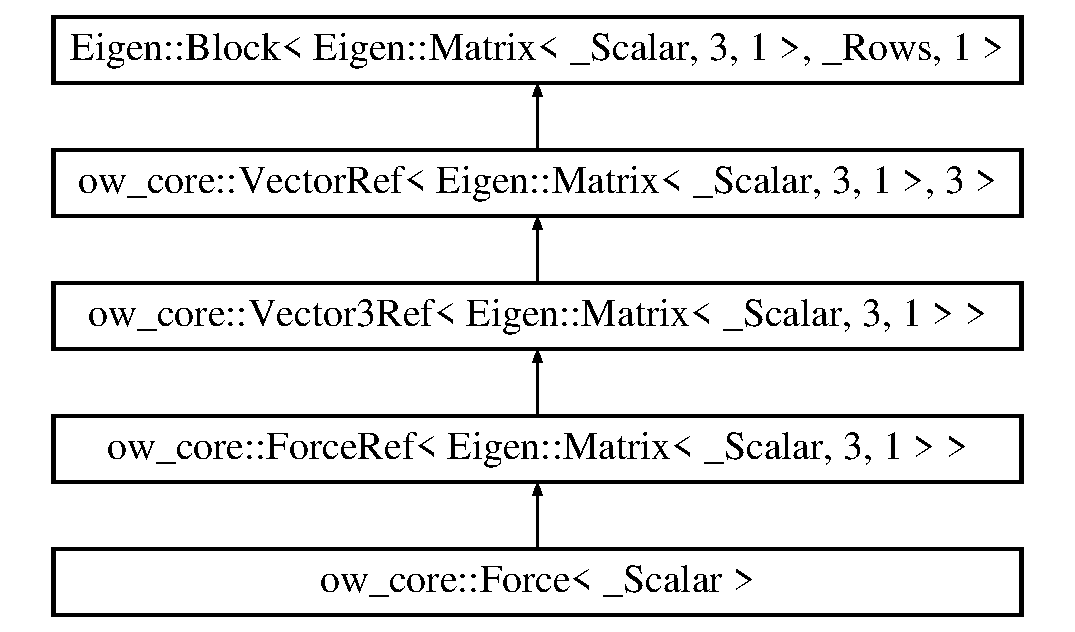
\includegraphics[height=5.000000cm]{d5/d29/classow__core_1_1Force}
\end{center}
\end{figure}
\subsection*{Public Types}
\begin{DoxyCompactItemize}
\item 
typedef \+\_\+\+Scalar {\bfseries Scalar}\hypertarget{classow__core_1_1Force_a551a42903f5645dd058650d0205586bf}{}\label{classow__core_1_1Force_a551a42903f5645dd058650d0205586bf}

\item 
typedef Eigen\+::\+Matrix$<$ \+\_\+\+Scalar, 3, 1 $>$ {\bfseries Derived}\hypertarget{classow__core_1_1Force_a2b611f8d302b86c6dcb045e9d3b24b75}{}\label{classow__core_1_1Force_a2b611f8d302b86c6dcb045e9d3b24b75}

\item 
typedef \hyperlink{classow__core_1_1ForceRef}{Force\+Ref}$<$ Derived $>$ {\bfseries Base}\hypertarget{classow__core_1_1Force_a3d10d556af18cc56227ddca163044d0c}{}\label{classow__core_1_1Force_a3d10d556af18cc56227ddca163044d0c}

\end{DoxyCompactItemize}
\subsection*{Public Member Functions}
\begin{DoxyCompactItemize}
\item 
\hyperlink{classow__core_1_1Force_ab6ef4b86db1e7e9a6f87ec6f71eb6d70}{Force} ()\hypertarget{classow__core_1_1Force_ab6ef4b86db1e7e9a6f87ec6f71eb6d70}{}\label{classow__core_1_1Force_ab6ef4b86db1e7e9a6f87ec6f71eb6d70}

\begin{DoxyCompactList}\small\item\em Default Constructor. \end{DoxyCompactList}\item 
\hyperlink{classow__core_1_1Force_a59f02d31c749b20c4d8f9a75c12648bd}{Force} (const Scalar \&x, const Scalar \&y, const Scalar \&z)\hypertarget{classow__core_1_1Force_a59f02d31c749b20c4d8f9a75c12648bd}{}\label{classow__core_1_1Force_a59f02d31c749b20c4d8f9a75c12648bd}

\begin{DoxyCompactList}\small\item\em Assignment from Scalar values. \end{DoxyCompactList}\item 
{\footnotesize template$<$typename Other\+Derived $>$ }\\\hyperlink{classow__core_1_1Force_a18c51f9e8b1fa8dbeada59438110aa97}{Force} (const Eigen\+::\+Eigen\+Base$<$ Other\+Derived $>$ \&other)
\begin{DoxyCompactList}\small\item\em Copy constructor. \end{DoxyCompactList}\end{DoxyCompactItemize}
\subsection*{Protected Attributes}
\begin{DoxyCompactItemize}
\item 
Derived {\bfseries data\+\_\+}\hypertarget{classow__core_1_1Force_af945fade7b7a37dfb0c86406b5794e7e}{}\label{classow__core_1_1Force_af945fade7b7a37dfb0c86406b5794e7e}

\end{DoxyCompactItemize}


\subsection{Detailed Description}
\subsubsection*{template$<$typename \+\_\+\+Scalar$>$\\*
class ow\+\_\+core\+::\+Force$<$ \+\_\+\+Scalar $>$}

The \hyperlink{classow__core_1_1ForceRef}{Force\+Ref} class. 

The \hyperlink{classow__core_1_1ForceRef}{Force\+Ref} is of type Eigen\+::\+Vector3 and is represented by the math symbol $\mathbf{f}$. 

\subsection{Constructor \& Destructor Documentation}
\index{ow\+\_\+core\+::\+Force@{ow\+\_\+core\+::\+Force}!Force@{Force}}
\index{Force@{Force}!ow\+\_\+core\+::\+Force@{ow\+\_\+core\+::\+Force}}
\subsubsection[{\texorpdfstring{Force(const Eigen\+::\+Eigen\+Base$<$ Other\+Derived $>$ \&other)}{Force(const Eigen::EigenBase< OtherDerived > &other)}}]{\setlength{\rightskip}{0pt plus 5cm}template$<$typename \+\_\+\+Scalar $>$ template$<$typename Other\+Derived $>$ {\bf ow\+\_\+core\+::\+Force}$<$ \+\_\+\+Scalar $>$\+::{\bf Force} (
\begin{DoxyParamCaption}
\item[{const Eigen\+::\+Eigen\+Base$<$ Other\+Derived $>$ \&}]{other}
\end{DoxyParamCaption}
)\hspace{0.3cm}{\ttfamily [inline]}}\hypertarget{classow__core_1_1Force_a18c51f9e8b1fa8dbeada59438110aa97}{}\label{classow__core_1_1Force_a18c51f9e8b1fa8dbeada59438110aa97}


Copy constructor. 

This copy constructor not only works with Eigen matrices but also with their expressions. 

The documentation for this class was generated from the following file\+:\begin{DoxyCompactItemize}
\item 
/home/dean/ros/workspaces/ow\+\_\+test\+\_\+ws/src/ow\+\_\+core/include/ow\+\_\+core/\hyperlink{force_8h}{force.\+h}\end{DoxyCompactItemize}

\hypertarget{classow__core_1_1ForceRef}{}\section{ow\+\_\+core\+:\+:Force\+Ref$<$ \+\_\+\+Derived $>$ Class Template Reference}
\label{classow__core_1_1ForceRef}\index{ow\+\_\+core\+::\+Force\+Ref$<$ \+\_\+\+Derived $>$@{ow\+\_\+core\+::\+Force\+Ref$<$ \+\_\+\+Derived $>$}}


The \hyperlink{classow__core_1_1ForceRef}{Force\+Ref} class.  




{\ttfamily \#include $<$force\+\_\+ref.\+h$>$}

Inheritance diagram for ow\+\_\+core\+:\+:Force\+Ref$<$ \+\_\+\+Derived $>$\+:\begin{figure}[H]
\begin{center}
\leavevmode
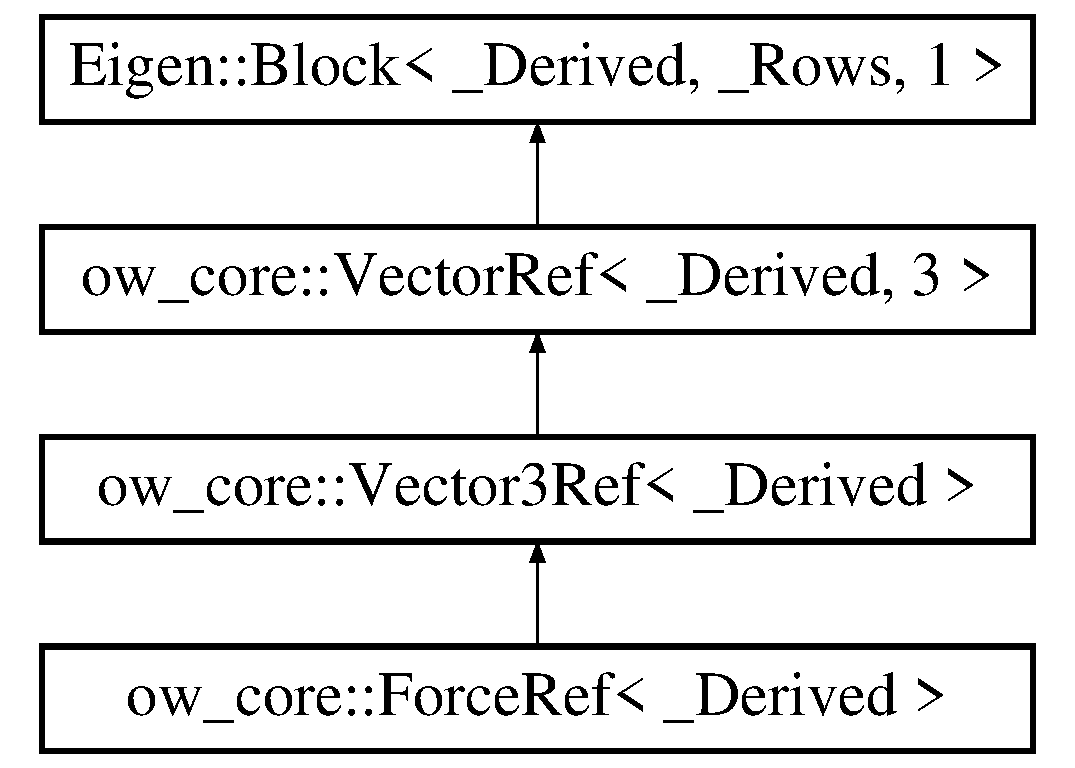
\includegraphics[height=4.000000cm]{d8/d3c/classow__core_1_1ForceRef}
\end{center}
\end{figure}
\subsection*{Public Types}
\begin{DoxyCompactItemize}
\item 
typedef \+\_\+\+Derived {\bfseries Derived}\hypertarget{classow__core_1_1ForceRef_a3f6e6ffbeb09f4aa9f9bb0708ea78413}{}\label{classow__core_1_1ForceRef_a3f6e6ffbeb09f4aa9f9bb0708ea78413}

\item 
typedef \hyperlink{classow__core_1_1Vector3Ref}{Vector3\+Ref}$<$ Derived $>$ {\bfseries Base}\hypertarget{classow__core_1_1ForceRef_a652bcc66be4d4ff071c4a6468b9da76c}{}\label{classow__core_1_1ForceRef_a652bcc66be4d4ff071c4a6468b9da76c}

\end{DoxyCompactItemize}
\subsection*{Public Member Functions}
\begin{DoxyCompactItemize}
\item 
\hyperlink{classow__core_1_1ForceRef_a30cace6ce8c34e20064bb2db164105f3}{Force\+Ref} (Derived \&ref, int start\+Row=0, int start\+Col=0)
\begin{DoxyCompactList}\small\item\em Default Constructor. \end{DoxyCompactList}\end{DoxyCompactItemize}


\subsection{Detailed Description}
\subsubsection*{template$<$typename \+\_\+\+Derived$>$\\*
class ow\+\_\+core\+::\+Force\+Ref$<$ \+\_\+\+Derived $>$}

The \hyperlink{classow__core_1_1ForceRef}{Force\+Ref} class. 

The \hyperlink{classow__core_1_1ForceRef}{Force\+Ref} is of type Eigen\+::\+Vector3 and is represented by the math symbol $\mathbf{f}$.

References the data of another Eigen type class via Eigen\+::\+Block. 

\subsection{Constructor \& Destructor Documentation}
\index{ow\+\_\+core\+::\+Force\+Ref@{ow\+\_\+core\+::\+Force\+Ref}!Force\+Ref@{Force\+Ref}}
\index{Force\+Ref@{Force\+Ref}!ow\+\_\+core\+::\+Force\+Ref@{ow\+\_\+core\+::\+Force\+Ref}}
\subsubsection[{\texorpdfstring{Force\+Ref(\+Derived \&ref, int start\+Row=0, int start\+Col=0)}{ForceRef(Derived &ref, int startRow=0, int startCol=0)}}]{\setlength{\rightskip}{0pt plus 5cm}template$<$typename \+\_\+\+Derived$>$ {\bf ow\+\_\+core\+::\+Force\+Ref}$<$ \+\_\+\+Derived $>$\+::{\bf Force\+Ref} (
\begin{DoxyParamCaption}
\item[{Derived \&}]{ref, }
\item[{int}]{start\+Row = {\ttfamily 0}, }
\item[{int}]{start\+Col = {\ttfamily 0}}
\end{DoxyParamCaption}
)\hspace{0.3cm}{\ttfamily [inline]}, {\ttfamily [explicit]}}\hypertarget{classow__core_1_1ForceRef_a30cace6ce8c34e20064bb2db164105f3}{}\label{classow__core_1_1ForceRef_a30cace6ce8c34e20064bb2db164105f3}


Default Constructor. 


\begin{DoxyParams}{Parameters}
{\em ref} & the reference to storage Eigen object to access the elements of the Linear\+Velocityn via Eigen\+::\+Block.\\
\hline
{\em start\+Row} & the start index of the row for Eigen\+::\+Block.\\
\hline
{\em start\+Col} & the start index of the column for Eigen\+::\+Block. \\
\hline
\end{DoxyParams}


The documentation for this class was generated from the following file\+:\begin{DoxyCompactItemize}
\item 
/home/dean/ros/workspaces/ow\+\_\+test\+\_\+ws/src/ow\+\_\+core/include/ow\+\_\+core/\hyperlink{force__ref_8h}{force\+\_\+ref.\+h}\end{DoxyCompactItemize}

\hypertarget{classow__core_1_1ForceTorqueSensors}{}\section{ow\+\_\+core\+:\+:Force\+Torque\+Sensors Class Reference}
\label{classow__core_1_1ForceTorqueSensors}\index{ow\+\_\+core\+::\+Force\+Torque\+Sensors@{ow\+\_\+core\+::\+Force\+Torque\+Sensors}}


The \hyperlink{classow__core_1_1ForceTorqueSensors}{Force\+Torque\+Sensors} class.  




{\ttfamily \#include $<$force\+\_\+torque\+\_\+sensors.\+h$>$}

Inheritance diagram for ow\+\_\+core\+:\+:Force\+Torque\+Sensors\+:\begin{figure}[H]
\begin{center}
\leavevmode
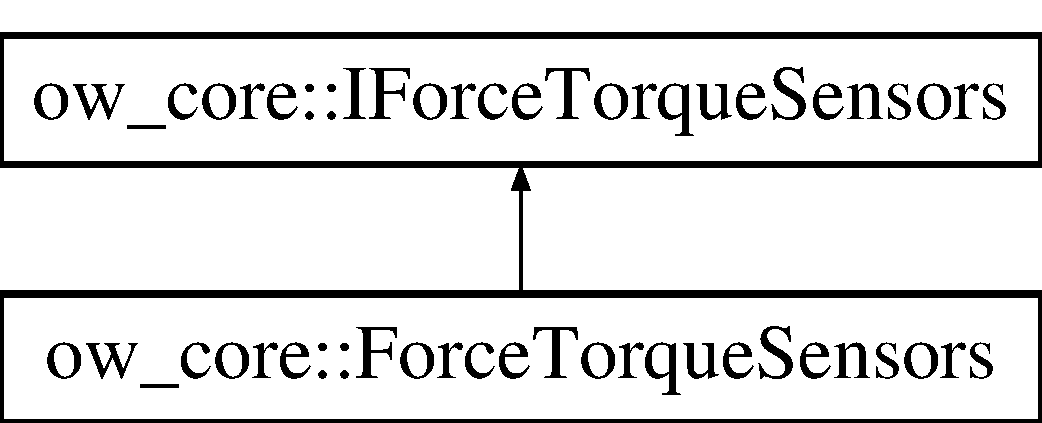
\includegraphics[height=2.000000cm]{de/d94/classow__core_1_1ForceTorqueSensors}
\end{center}
\end{figure}
\subsection*{Public Member Functions}
\begin{DoxyCompactItemize}
\item 
virtual \hyperlink{classow__core_1_1ForceTorqueSensors_a9872e14ea1b6b503f4eef0f17222eb57}{$\sim$\+Force\+Torque\+Sensors} ()\hypertarget{classow__core_1_1ForceTorqueSensors_a9872e14ea1b6b503f4eef0f17222eb57}{}\label{classow__core_1_1ForceTorqueSensors_a9872e14ea1b6b503f4eef0f17222eb57}

\begin{DoxyCompactList}\small\item\em Virtual destructor. \end{DoxyCompactList}\item 
virtual \hyperlink{classow__core_1_1Wrench}{ow\+::\+Wrench} \& {\bfseries left\+Foot} ()\hypertarget{classow__core_1_1ForceTorqueSensors_a45ed561bd8b97569e16b9ef5ae46a073}{}\label{classow__core_1_1ForceTorqueSensors_a45ed561bd8b97569e16b9ef5ae46a073}

\item 
virtual const \hyperlink{classow__core_1_1Wrench}{ow\+::\+Wrench} \& {\bfseries left\+Foot} () const \hypertarget{classow__core_1_1ForceTorqueSensors_a7fed26b5f54f39730d0eca7145585d3e}{}\label{classow__core_1_1ForceTorqueSensors_a7fed26b5f54f39730d0eca7145585d3e}

\item 
virtual \hyperlink{classow__core_1_1Wrench}{ow\+::\+Wrench} \& {\bfseries right\+Foot} ()\hypertarget{classow__core_1_1ForceTorqueSensors_a7093ca53c0ab93e2ad274e8bf03313bf}{}\label{classow__core_1_1ForceTorqueSensors_a7093ca53c0ab93e2ad274e8bf03313bf}

\item 
virtual const \hyperlink{classow__core_1_1Wrench}{ow\+::\+Wrench} \& {\bfseries right\+Foot} () const \hypertarget{classow__core_1_1ForceTorqueSensors_aad0539d24a54f5cb111cbdbaf6ff4f35}{}\label{classow__core_1_1ForceTorqueSensors_aad0539d24a54f5cb111cbdbaf6ff4f35}

\end{DoxyCompactItemize}
\subsection*{Protected Attributes}
\begin{DoxyCompactItemize}
\item 
\hyperlink{classow__core_1_1Wrench}{ow\+::\+Wrench} {\bfseries left\+Foot\+\_\+}\hypertarget{classow__core_1_1ForceTorqueSensors_a89fd5dd2e34a98cc2e2902e357ec9432}{}\label{classow__core_1_1ForceTorqueSensors_a89fd5dd2e34a98cc2e2902e357ec9432}

\item 
\hyperlink{classow__core_1_1Wrench}{ow\+::\+Wrench} {\bfseries right\+Foot\+\_\+}\hypertarget{classow__core_1_1ForceTorqueSensors_a9cb8c802cfc5bd1e110abf12a101b2af}{}\label{classow__core_1_1ForceTorqueSensors_a9cb8c802cfc5bd1e110abf12a101b2af}

\end{DoxyCompactItemize}


\subsection{Detailed Description}
The \hyperlink{classow__core_1_1ForceTorqueSensors}{Force\+Torque\+Sensors} class. 

The default implementation of the \hyperlink{classow__core_1_1IForceTorqueSensors}{I\+Force\+Torque\+Sensors} interface. 

The documentation for this class was generated from the following file\+:\begin{DoxyCompactItemize}
\item 
/home/dean/ros/workspaces/ow\+\_\+test\+\_\+ws/src/ow\+\_\+core/include/ow\+\_\+core/\+Implementations/\hyperlink{force__torque__sensors_8h}{force\+\_\+torque\+\_\+sensors.\+h}\end{DoxyCompactItemize}

\hypertarget{classow__core_1_1HomogeneousTransformation}{}\section{ow\+\_\+core\+:\+:Homogeneous\+Transformation$<$ \+\_\+\+Scalar $>$ Class Template Reference}
\label{classow__core_1_1HomogeneousTransformation}\index{ow\+\_\+core\+::\+Homogeneous\+Transformation$<$ \+\_\+\+Scalar $>$@{ow\+\_\+core\+::\+Homogeneous\+Transformation$<$ \+\_\+\+Scalar $>$}}


The \hyperlink{classow__core_1_1HomogeneousTransformation}{Homogeneous\+Transformation} class.  




{\ttfamily \#include $<$homogeneous\+\_\+transformation.\+h$>$}

Inheritance diagram for ow\+\_\+core\+:\+:Homogeneous\+Transformation$<$ \+\_\+\+Scalar $>$\+:\begin{figure}[H]
\begin{center}
\leavevmode
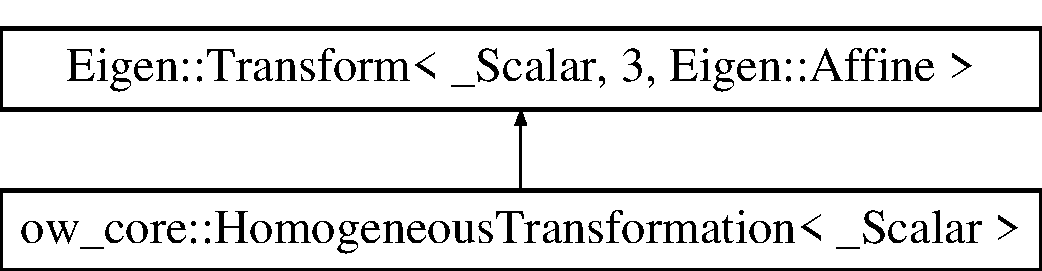
\includegraphics[height=2.000000cm]{d5/de4/classow__core_1_1HomogeneousTransformation}
\end{center}
\end{figure}
\subsection*{Public Types}
\begin{DoxyCompactItemize}
\item 
typedef \+\_\+\+Scalar {\bfseries Scalar}\hypertarget{classow__core_1_1HomogeneousTransformation_a831cf394e7c5ef71aa2384c942d353cc}{}\label{classow__core_1_1HomogeneousTransformation_a831cf394e7c5ef71aa2384c942d353cc}

\item 
typedef Eigen\+::\+Transform$<$ \+\_\+\+Scalar, 3, Eigen\+::\+Affine $>$ {\bfseries Base}\hypertarget{classow__core_1_1HomogeneousTransformation_a139a040b2aaf4205cd2ee48efcda3a5a}{}\label{classow__core_1_1HomogeneousTransformation_a139a040b2aaf4205cd2ee48efcda3a5a}

\item 
typedef Eigen\+::\+Transform$<$ \+\_\+\+Scalar, 3, Eigen\+::\+Affine $>$\+::Matrix\+Type {\bfseries Matrix}\hypertarget{classow__core_1_1HomogeneousTransformation_a1ce471e38a5056c8e97409a1c3bd9798}{}\label{classow__core_1_1HomogeneousTransformation_a1ce471e38a5056c8e97409a1c3bd9798}

\end{DoxyCompactItemize}
\subsection*{Public Member Functions}
\begin{DoxyCompactItemize}
\item 
\hyperlink{classow__core_1_1HomogeneousTransformation_a6a2d52fc4ee38abbe480a6d5a8e5c773}{Homogeneous\+Transformation} ()\hypertarget{classow__core_1_1HomogeneousTransformation_a6a2d52fc4ee38abbe480a6d5a8e5c773}{}\label{classow__core_1_1HomogeneousTransformation_a6a2d52fc4ee38abbe480a6d5a8e5c773}

\begin{DoxyCompactList}\small\item\em Default Constructor. \end{DoxyCompactList}\item 
\hyperlink{classow__core_1_1HomogeneousTransformation_ac1d8792424c0af25dffd0c7e38981caa}{Homogeneous\+Transformation} (const Base \&other)
\begin{DoxyCompactList}\small\item\em Copy constructor from Eigen\+::\+Affine. \end{DoxyCompactList}\item 
{\footnotesize template$<$typename Other\+Derived $>$ }\\\hyperlink{classow__core_1_1HomogeneousTransformation_a453016dcb8a706ffb95abfd60a70f1df}{Homogeneous\+Transformation} (const Eigen\+::\+Eigen\+Base$<$ Other\+Derived $>$ \&other)
\begin{DoxyCompactList}\small\item\em Copy constructor Other\+Derived. \end{DoxyCompactList}\item 
\hyperlink{classow__core_1_1HomogeneousTransformation_a9def3964364fb962d1a69fe06686ee9e}{Homogeneous\+Transformation} (const typename Base\+::\+Translation\+Type \&other)\hypertarget{classow__core_1_1HomogeneousTransformation_a9def3964364fb962d1a69fe06686ee9e}{}\label{classow__core_1_1HomogeneousTransformation_a9def3964364fb962d1a69fe06686ee9e}

\begin{DoxyCompactList}\small\item\em Copy constructor from Eigen\+::\+Transform\+::\+Translation. \end{DoxyCompactList}\item 
{\footnotesize template$<$typename Other\+Derived $>$ }\\\hyperlink{classow__core_1_1HomogeneousTransformation_a8ebeed0581c35b89d96a847f01bceddb}{Homogeneous\+Transformation} (const Eigen\+::\+Rotation\+Base$<$ Other\+Derived, 3 $>$ \&other)\hypertarget{classow__core_1_1HomogeneousTransformation_a8ebeed0581c35b89d96a847f01bceddb}{}\label{classow__core_1_1HomogeneousTransformation_a8ebeed0581c35b89d96a847f01bceddb}

\begin{DoxyCompactList}\small\item\em Copy constructor from Eigen\+::\+Rotation\+Base. \end{DoxyCompactList}\item 
\hyperlink{classow__core_1_1HomogeneousTransformation_a93c036ece8c23ef2fc7a9d38a59ff7e8}{Homogeneous\+Transformation} (const tf\+::\+Transform \&other)\hypertarget{classow__core_1_1HomogeneousTransformation_a93c036ece8c23ef2fc7a9d38a59ff7e8}{}\label{classow__core_1_1HomogeneousTransformation_a93c036ece8c23ef2fc7a9d38a59ff7e8}

\begin{DoxyCompactList}\small\item\em Copy constructor from tf\+::\+Transform. \end{DoxyCompactList}\item 
\hyperlink{classow__core_1_1HomogeneousTransformation_af4078447d97d97921a1cde705c661228}{Homogeneous\+Transformation} (const geometry\+\_\+msgs\+::\+Pose \&other)\hypertarget{classow__core_1_1HomogeneousTransformation_af4078447d97d97921a1cde705c661228}{}\label{classow__core_1_1HomogeneousTransformation_af4078447d97d97921a1cde705c661228}

\begin{DoxyCompactList}\small\item\em Copy constructor from geometry\+\_\+msgs\+::\+Pose. \end{DoxyCompactList}\item 
void \hyperlink{classow__core_1_1HomogeneousTransformation_a52c2ab8ad47f43b8c94a7d5576e8c842}{operator=} (const tf\+::\+Transform \&other)\hypertarget{classow__core_1_1HomogeneousTransformation_a52c2ab8ad47f43b8c94a7d5576e8c842}{}\label{classow__core_1_1HomogeneousTransformation_a52c2ab8ad47f43b8c94a7d5576e8c842}

\begin{DoxyCompactList}\small\item\em Assignment form tf\+::\+Transform. \end{DoxyCompactList}\item 
void \hyperlink{classow__core_1_1HomogeneousTransformation_a020a141fc151737a9671df9448e954a9}{operator=} (const geometry\+\_\+msgs\+::\+Pose \&other)\hypertarget{classow__core_1_1HomogeneousTransformation_a020a141fc151737a9671df9448e954a9}{}\label{classow__core_1_1HomogeneousTransformation_a020a141fc151737a9671df9448e954a9}

\begin{DoxyCompactList}\small\item\em Assignment form geometry\+\_\+msgs\+::\+Pose. \end{DoxyCompactList}\item 
\hyperlink{classow__core_1_1HomogeneousTransformation_a223412eca2309326b0f672a38c1e6a44}{operator tf\+::\+Transform} () const \hypertarget{classow__core_1_1HomogeneousTransformation_a223412eca2309326b0f672a38c1e6a44}{}\label{classow__core_1_1HomogeneousTransformation_a223412eca2309326b0f672a38c1e6a44}

\begin{DoxyCompactList}\small\item\em Conversion to tf\+::\+Transform. \end{DoxyCompactList}\item 
\hyperlink{classow__core_1_1HomogeneousTransformation_ad92f1c9512c6fcc000ac73abdba5a103}{operator geometry\+\_\+msgs\+::\+Pose} () const \hypertarget{classow__core_1_1HomogeneousTransformation_ad92f1c9512c6fcc000ac73abdba5a103}{}\label{classow__core_1_1HomogeneousTransformation_ad92f1c9512c6fcc000ac73abdba5a103}

\begin{DoxyCompactList}\small\item\em Conversion to geometry\+\_\+msgs\+::\+Pose. \end{DoxyCompactList}\item 
tf\+::\+Transform \hyperlink{classow__core_1_1HomogeneousTransformation_aeaf8eff278df891b098ea4bf1ce81cc9}{to\+Transform\+Tf} ()\hypertarget{classow__core_1_1HomogeneousTransformation_aeaf8eff278df891b098ea4bf1ce81cc9}{}\label{classow__core_1_1HomogeneousTransformation_aeaf8eff278df891b098ea4bf1ce81cc9}

\begin{DoxyCompactList}\small\item\em Conversion to tf\+::\+Transform. \end{DoxyCompactList}\item 
geometry\+\_\+msgs\+::\+Pose \hyperlink{classow__core_1_1HomogeneousTransformation_a32bd1fa2962cc71f8331fcfc39d55b2e}{to\+Pose\+Msg} ()\hypertarget{classow__core_1_1HomogeneousTransformation_a32bd1fa2962cc71f8331fcfc39d55b2e}{}\label{classow__core_1_1HomogeneousTransformation_a32bd1fa2962cc71f8331fcfc39d55b2e}

\begin{DoxyCompactList}\small\item\em Conversion to geometry\+\_\+msgs\+::\+Pose. \end{DoxyCompactList}\item 
\hyperlink{classow__core_1_1LinearPositionRef}{Linear\+Position\+Ref}$<$ Matrix $>$ \hyperlink{classow__core_1_1HomogeneousTransformation_a45c97f141777f691dbed43420d7d43e3}{position} ()\hypertarget{classow__core_1_1HomogeneousTransformation_a45c97f141777f691dbed43420d7d43e3}{}\label{classow__core_1_1HomogeneousTransformation_a45c97f141777f691dbed43420d7d43e3}

\begin{DoxyCompactList}\small\item\em access to position part \end{DoxyCompactList}\item 
\hyperlink{classow__core_1_1LinearPositionRef}{Linear\+Position\+Ref}$<$ const Matrix $>$ \hyperlink{classow__core_1_1HomogeneousTransformation_ae2eecf2fd172b4da05031f94d3d050a7}{position} () const \hypertarget{classow__core_1_1HomogeneousTransformation_ae2eecf2fd172b4da05031f94d3d050a7}{}\label{classow__core_1_1HomogeneousTransformation_ae2eecf2fd172b4da05031f94d3d050a7}

\begin{DoxyCompactList}\small\item\em const access to position part \end{DoxyCompactList}\item 
\hyperlink{classow__core_1_1Rotation3Ref}{Rotation3\+Ref}$<$ Matrix $>$ \hyperlink{classow__core_1_1HomogeneousTransformation_aae6ef9088cc07bfa5e3b76de5b2f9ede}{orientation} ()\hypertarget{classow__core_1_1HomogeneousTransformation_aae6ef9088cc07bfa5e3b76de5b2f9ede}{}\label{classow__core_1_1HomogeneousTransformation_aae6ef9088cc07bfa5e3b76de5b2f9ede}

\begin{DoxyCompactList}\small\item\em access to orientation part \end{DoxyCompactList}\item 
\hyperlink{classow__core_1_1Rotation3Ref}{Rotation3\+Ref}$<$ const Matrix $>$ \hyperlink{classow__core_1_1HomogeneousTransformation_ab2dcd67527042fd99a7f47f539497cb8}{orientation} () const \hypertarget{classow__core_1_1HomogeneousTransformation_ab2dcd67527042fd99a7f47f539497cb8}{}\label{classow__core_1_1HomogeneousTransformation_ab2dcd67527042fd99a7f47f539497cb8}

\begin{DoxyCompactList}\small\item\em const access to orientation part \end{DoxyCompactList}\item 
std\+::string \hyperlink{classow__core_1_1HomogeneousTransformation_a81377744bf29c6001680abdcd0f22f95}{to\+String} () const \hypertarget{classow__core_1_1HomogeneousTransformation_a81377744bf29c6001680abdcd0f22f95}{}\label{classow__core_1_1HomogeneousTransformation_a81377744bf29c6001680abdcd0f22f95}

\begin{DoxyCompactList}\small\item\em Conversion to std\+::string. \end{DoxyCompactList}\end{DoxyCompactItemize}
\subsection*{Static Public Member Functions}
\begin{DoxyCompactItemize}
\item 
static const \hyperlink{classow__core_1_1HomogeneousTransformation}{Homogeneous\+Transformation}$<$ Scalar $>$ \& \hyperlink{classow__core_1_1HomogeneousTransformation_a7113d1a0875f4c8583321a7f3aeb7740}{Default} ()
\begin{DoxyCompactList}\small\item\em Default constructor. \end{DoxyCompactList}\end{DoxyCompactItemize}


\subsection{Detailed Description}
\subsubsection*{template$<$typename \+\_\+\+Scalar$>$\\*
class ow\+\_\+core\+::\+Homogeneous\+Transformation$<$ \+\_\+\+Scalar $>$}

The \hyperlink{classow__core_1_1HomogeneousTransformation}{Homogeneous\+Transformation} class. 

The \hyperlink{classow__core_1_1HomogeneousTransformation}{Homogeneous\+Transformation} is of type Eigen\+::\+Transform and is represented by the math symbol $\mathbf{T}$.

Stores the position and orientation information in a 4x4 dimensional matrix. The orientation part is represented as a 3x3 matrix in the upper left corner. The position part is represented as a 3 dimensional vector in the upper right corner. 

\subsection{Constructor \& Destructor Documentation}
\index{ow\+\_\+core\+::\+Homogeneous\+Transformation@{ow\+\_\+core\+::\+Homogeneous\+Transformation}!Homogeneous\+Transformation@{Homogeneous\+Transformation}}
\index{Homogeneous\+Transformation@{Homogeneous\+Transformation}!ow\+\_\+core\+::\+Homogeneous\+Transformation@{ow\+\_\+core\+::\+Homogeneous\+Transformation}}
\subsubsection[{\texorpdfstring{Homogeneous\+Transformation(const Base \&other)}{HomogeneousTransformation(const Base &other)}}]{\setlength{\rightskip}{0pt plus 5cm}template$<$typename \+\_\+\+Scalar $>$ {\bf ow\+\_\+core\+::\+Homogeneous\+Transformation}$<$ \+\_\+\+Scalar $>$\+::{\bf Homogeneous\+Transformation} (
\begin{DoxyParamCaption}
\item[{const Base \&}]{other}
\end{DoxyParamCaption}
)\hspace{0.3cm}{\ttfamily [inline]}}\hypertarget{classow__core_1_1HomogeneousTransformation_ac1d8792424c0af25dffd0c7e38981caa}{}\label{classow__core_1_1HomogeneousTransformation_ac1d8792424c0af25dffd0c7e38981caa}


Copy constructor from Eigen\+::\+Affine. 

\begin{DoxyRefDesc}{Todo}
\item[\hyperlink{todo__todo000007}{Todo}]removed explicit to write\+: \hyperlink{classow__core_1_1HomogeneousTransformation}{Homogeneous\+Transformation} T = Eigen\+::\+Affine(...); \end{DoxyRefDesc}
\index{ow\+\_\+core\+::\+Homogeneous\+Transformation@{ow\+\_\+core\+::\+Homogeneous\+Transformation}!Homogeneous\+Transformation@{Homogeneous\+Transformation}}
\index{Homogeneous\+Transformation@{Homogeneous\+Transformation}!ow\+\_\+core\+::\+Homogeneous\+Transformation@{ow\+\_\+core\+::\+Homogeneous\+Transformation}}
\subsubsection[{\texorpdfstring{Homogeneous\+Transformation(const Eigen\+::\+Eigen\+Base$<$ Other\+Derived $>$ \&other)}{HomogeneousTransformation(const Eigen::EigenBase< OtherDerived > &other)}}]{\setlength{\rightskip}{0pt plus 5cm}template$<$typename \+\_\+\+Scalar $>$ template$<$typename Other\+Derived $>$ {\bf ow\+\_\+core\+::\+Homogeneous\+Transformation}$<$ \+\_\+\+Scalar $>$\+::{\bf Homogeneous\+Transformation} (
\begin{DoxyParamCaption}
\item[{const Eigen\+::\+Eigen\+Base$<$ Other\+Derived $>$ \&}]{other}
\end{DoxyParamCaption}
)\hspace{0.3cm}{\ttfamily [inline]}}\hypertarget{classow__core_1_1HomogeneousTransformation_a453016dcb8a706ffb95abfd60a70f1df}{}\label{classow__core_1_1HomogeneousTransformation_a453016dcb8a706ffb95abfd60a70f1df}


Copy constructor Other\+Derived. 

This copy constructor not only works with Eigen matrices but also with their expressions. 

\subsection{Member Function Documentation}
\index{ow\+\_\+core\+::\+Homogeneous\+Transformation@{ow\+\_\+core\+::\+Homogeneous\+Transformation}!Default@{Default}}
\index{Default@{Default}!ow\+\_\+core\+::\+Homogeneous\+Transformation@{ow\+\_\+core\+::\+Homogeneous\+Transformation}}
\subsubsection[{\texorpdfstring{Default()}{Default()}}]{\setlength{\rightskip}{0pt plus 5cm}template$<$typename \+\_\+\+Scalar $>$ static const {\bf Homogeneous\+Transformation}$<$Scalar$>$\& {\bf ow\+\_\+core\+::\+Homogeneous\+Transformation}$<$ \+\_\+\+Scalar $>$\+::Default (
\begin{DoxyParamCaption}
{}
\end{DoxyParamCaption}
)\hspace{0.3cm}{\ttfamily [inline]}, {\ttfamily [static]}}\hypertarget{classow__core_1_1HomogeneousTransformation_a7113d1a0875f4c8583321a7f3aeb7740}{}\label{classow__core_1_1HomogeneousTransformation_a7113d1a0875f4c8583321a7f3aeb7740}


Default constructor. 

constructs as identity 

The documentation for this class was generated from the following file\+:\begin{DoxyCompactItemize}
\item 
/home/dean/ros/workspaces/ow\+\_\+test\+\_\+ws/src/ow\+\_\+core/include/ow\+\_\+core/\hyperlink{homogeneous__transformation_8h}{homogeneous\+\_\+transformation.\+h}\end{DoxyCompactItemize}

\hypertarget{classow__core_1_1IFootTrajectoryGenerator}{}\section{ow\+\_\+core\+:\+:I\+Foot\+Trajectory\+Generator Class Reference}
\label{classow__core_1_1IFootTrajectoryGenerator}\index{ow\+\_\+core\+::\+I\+Foot\+Trajectory\+Generator@{ow\+\_\+core\+::\+I\+Foot\+Trajectory\+Generator}}


The \hyperlink{classow__core_1_1IFootTrajectoryGenerator}{I\+Foot\+Trajectory\+Generator} class.  




{\ttfamily \#include $<$i\+\_\+foot\+\_\+trajectory\+\_\+generator.\+h$>$}

\subsection*{Public Member Functions}
\begin{DoxyCompactItemize}
\item 
virtual \hyperlink{classow__core_1_1IFootTrajectoryGenerator_a67087027cedeb175cf41c5e7eacc8e87}{$\sim$\+I\+Foot\+Trajectory\+Generator} ()\hypertarget{classow__core_1_1IFootTrajectoryGenerator_a67087027cedeb175cf41c5e7eacc8e87}{}\label{classow__core_1_1IFootTrajectoryGenerator_a67087027cedeb175cf41c5e7eacc8e87}

\begin{DoxyCompactList}\small\item\em Virtual destructor. \end{DoxyCompactList}\item 
virtual \hyperlink{classow__core_1_1IFootTrajectoryGenerator_ac18698993d68a408ecb0820b1ce0cf4e}{connect\+In\+Port\+Foot\+Step\+Planner} (const I\+Foot\+Step\+Planner\+Out\+Ports $\ast$fsp)=0
\begin{DoxyCompactList}\small\item\em Connect to in port. \end{DoxyCompactList}\item 
virtual \hyperlink{classow__core_1_1IFootTrajectoryGenerator_ae592f6abe58e94f8197a4b29d4f52b6d}{connect\+In\+Port\+Forward\+Kinematic} (const I\+Forward\+Kinematics\+Out\+Ports $\ast$fk)=0
\begin{DoxyCompactList}\small\item\em Connect to in port. \end{DoxyCompactList}\item 
virtual const \hyperlink{classow__core_1_1IFootTrajectoryGeneratorOutPorts}{I\+Foot\+Trajectory\+Generator\+Out\+Ports} $\ast$ \hyperlink{classow__core_1_1IFootTrajectoryGenerator_add02082c2d05777990753ce28449cf4c}{out\+Ports} () const =0
\begin{DoxyCompactList}\small\item\em provice out ports. \end{DoxyCompactList}\end{DoxyCompactItemize}


\subsection{Detailed Description}
The \hyperlink{classow__core_1_1IFootTrajectoryGenerator}{I\+Foot\+Trajectory\+Generator} class. 

Interface class.

\begin{DoxyRefDesc}{Todo}
\item[\hyperlink{todo__todo000008}{Todo}]Remove forward declarations. \end{DoxyRefDesc}


\subsection{Member Function Documentation}
\index{ow\+\_\+core\+::\+I\+Foot\+Trajectory\+Generator@{ow\+\_\+core\+::\+I\+Foot\+Trajectory\+Generator}!connect\+In\+Port\+Foot\+Step\+Planner@{connect\+In\+Port\+Foot\+Step\+Planner}}
\index{connect\+In\+Port\+Foot\+Step\+Planner@{connect\+In\+Port\+Foot\+Step\+Planner}!ow\+\_\+core\+::\+I\+Foot\+Trajectory\+Generator@{ow\+\_\+core\+::\+I\+Foot\+Trajectory\+Generator}}
\subsubsection[{\texorpdfstring{connect\+In\+Port\+Foot\+Step\+Planner(const I\+Foot\+Step\+Planner\+Out\+Ports $\ast$fsp)=0}{connectInPortFootStepPlanner(const IFootStepPlannerOutPorts *fsp)=0}}]{\setlength{\rightskip}{0pt plus 5cm}virtual ow\+\_\+core\+::\+I\+Foot\+Trajectory\+Generator\+::connect\+In\+Port\+Foot\+Step\+Planner (
\begin{DoxyParamCaption}
\item[{const I\+Foot\+Step\+Planner\+Out\+Ports $\ast$}]{fsp}
\end{DoxyParamCaption}
)\hspace{0.3cm}{\ttfamily [pure virtual]}}\hypertarget{classow__core_1_1IFootTrajectoryGenerator_ac18698993d68a408ecb0820b1ce0cf4e}{}\label{classow__core_1_1IFootTrajectoryGenerator_ac18698993d68a408ecb0820b1ce0cf4e}


Connect to in port. 

\begin{DoxyRefDesc}{Todo}
\item[\hyperlink{todo__todo000009}{Todo}]give specific pointer to other module ouput or the most general outport pointer?\end{DoxyRefDesc}


Connects this module to the out port of another module. \index{ow\+\_\+core\+::\+I\+Foot\+Trajectory\+Generator@{ow\+\_\+core\+::\+I\+Foot\+Trajectory\+Generator}!connect\+In\+Port\+Forward\+Kinematic@{connect\+In\+Port\+Forward\+Kinematic}}
\index{connect\+In\+Port\+Forward\+Kinematic@{connect\+In\+Port\+Forward\+Kinematic}!ow\+\_\+core\+::\+I\+Foot\+Trajectory\+Generator@{ow\+\_\+core\+::\+I\+Foot\+Trajectory\+Generator}}
\subsubsection[{\texorpdfstring{connect\+In\+Port\+Forward\+Kinematic(const I\+Forward\+Kinematics\+Out\+Ports $\ast$fk)=0}{connectInPortForwardKinematic(const IForwardKinematicsOutPorts *fk)=0}}]{\setlength{\rightskip}{0pt plus 5cm}virtual ow\+\_\+core\+::\+I\+Foot\+Trajectory\+Generator\+::connect\+In\+Port\+Forward\+Kinematic (
\begin{DoxyParamCaption}
\item[{const I\+Forward\+Kinematics\+Out\+Ports $\ast$}]{fk}
\end{DoxyParamCaption}
)\hspace{0.3cm}{\ttfamily [pure virtual]}}\hypertarget{classow__core_1_1IFootTrajectoryGenerator_ae592f6abe58e94f8197a4b29d4f52b6d}{}\label{classow__core_1_1IFootTrajectoryGenerator_ae592f6abe58e94f8197a4b29d4f52b6d}


Connect to in port. 

\begin{DoxyRefDesc}{Todo}
\item[\hyperlink{todo__todo000010}{Todo}]give specific pointer to other module ouput or the most general outport pointer?\end{DoxyRefDesc}


Connects this module to the out port of another module. \index{ow\+\_\+core\+::\+I\+Foot\+Trajectory\+Generator@{ow\+\_\+core\+::\+I\+Foot\+Trajectory\+Generator}!out\+Ports@{out\+Ports}}
\index{out\+Ports@{out\+Ports}!ow\+\_\+core\+::\+I\+Foot\+Trajectory\+Generator@{ow\+\_\+core\+::\+I\+Foot\+Trajectory\+Generator}}
\subsubsection[{\texorpdfstring{out\+Ports() const =0}{outPorts() const =0}}]{\setlength{\rightskip}{0pt plus 5cm}virtual const {\bf I\+Foot\+Trajectory\+Generator\+Out\+Ports}$\ast$ ow\+\_\+core\+::\+I\+Foot\+Trajectory\+Generator\+::out\+Ports (
\begin{DoxyParamCaption}
{}
\end{DoxyParamCaption}
) const\hspace{0.3cm}{\ttfamily [pure virtual]}}\hypertarget{classow__core_1_1IFootTrajectoryGenerator_add02082c2d05777990753ce28449cf4c}{}\label{classow__core_1_1IFootTrajectoryGenerator_add02082c2d05777990753ce28449cf4c}


provice out ports. 

Connects this module to the in port of another module. 

The documentation for this class was generated from the following file\+:\begin{DoxyCompactItemize}
\item 
/home/dean/ros/workspaces/ow\+\_\+test\+\_\+ws/src/ow\+\_\+core/include/ow\+\_\+core/\+Interfaces/\hyperlink{i__foot__trajectory__generator_8h}{i\+\_\+foot\+\_\+trajectory\+\_\+generator.\+h}\end{DoxyCompactItemize}

\hypertarget{classow__core_1_1IFootTrajectoryGeneratorOutPorts}{}\section{ow\+\_\+core\+:\+:I\+Foot\+Trajectory\+Generator\+Out\+Ports Class Reference}
\label{classow__core_1_1IFootTrajectoryGeneratorOutPorts}\index{ow\+\_\+core\+::\+I\+Foot\+Trajectory\+Generator\+Out\+Ports@{ow\+\_\+core\+::\+I\+Foot\+Trajectory\+Generator\+Out\+Ports}}


The \hyperlink{classow__core_1_1IFootTrajectoryGeneratorOutPorts}{I\+Foot\+Trajectory\+Generator\+Out\+Ports} class.  




{\ttfamily \#include $<$i\+\_\+foot\+\_\+trajectory\+\_\+generator\+\_\+out\+\_\+ports.\+h$>$}

\subsection*{Public Member Functions}
\begin{DoxyCompactItemize}
\item 
virtual \hyperlink{classow__core_1_1IFootTrajectoryGeneratorOutPorts_a259a736c18d31e618caa247ab733aee1}{$\sim$\+I\+Foot\+Trajectory\+Generator\+Out\+Ports} ()\hypertarget{classow__core_1_1IFootTrajectoryGeneratorOutPorts_a259a736c18d31e618caa247ab733aee1}{}\label{classow__core_1_1IFootTrajectoryGeneratorOutPorts_a259a736c18d31e618caa247ab733aee1}

\begin{DoxyCompactList}\small\item\em Virtual destructor. \end{DoxyCompactList}\item 
virtual \hyperlink{classow__core_1_1CartesianPosition}{ow\+::\+Cartesian\+Position} \& {\bfseries X} ()=0\hypertarget{classow__core_1_1IFootTrajectoryGeneratorOutPorts_abf512b870079271cf9fcaaf086ae5e6f}{}\label{classow__core_1_1IFootTrajectoryGeneratorOutPorts_abf512b870079271cf9fcaaf086ae5e6f}

\item 
virtual const \hyperlink{classow__core_1_1CartesianPosition}{ow\+::\+Cartesian\+Position} \& {\bfseries X} () const =0\hypertarget{classow__core_1_1IFootTrajectoryGeneratorOutPorts_a54eee4d69b68ce6222cf28ac6823d8be}{}\label{classow__core_1_1IFootTrajectoryGeneratorOutPorts_a54eee4d69b68ce6222cf28ac6823d8be}

\item 
virtual \hyperlink{classow__core_1_1CartesianVelocity}{ow\+::\+Cartesian\+Velocity} \& {\bfseries Xp} ()=0\hypertarget{classow__core_1_1IFootTrajectoryGeneratorOutPorts_ae5effc4d3521b914c5c3c19bf4b803a9}{}\label{classow__core_1_1IFootTrajectoryGeneratorOutPorts_ae5effc4d3521b914c5c3c19bf4b803a9}

\item 
virtual const \hyperlink{classow__core_1_1CartesianVelocity}{ow\+::\+Cartesian\+Velocity} \& {\bfseries Xp} () const =0\hypertarget{classow__core_1_1IFootTrajectoryGeneratorOutPorts_ad3ebd4f297c75f651ceec4080e1028dc}{}\label{classow__core_1_1IFootTrajectoryGeneratorOutPorts_ad3ebd4f297c75f651ceec4080e1028dc}

\item 
virtual \hyperlink{classow__core_1_1CartesianAcceleration}{ow\+::\+Cartesian\+Acceleration} \& {\bfseries Xpp} ()=0\hypertarget{classow__core_1_1IFootTrajectoryGeneratorOutPorts_a256480ac0645ca1517177b30e8b0abe0}{}\label{classow__core_1_1IFootTrajectoryGeneratorOutPorts_a256480ac0645ca1517177b30e8b0abe0}

\item 
virtual const \hyperlink{classow__core_1_1CartesianAcceleration}{ow\+::\+Cartesian\+Acceleration} \& {\bfseries Xpp} () const =0\hypertarget{classow__core_1_1IFootTrajectoryGeneratorOutPorts_a56cd6bd41e3ff6f1e8f8521144b801d6}{}\label{classow__core_1_1IFootTrajectoryGeneratorOutPorts_a56cd6bd41e3ff6f1e8f8521144b801d6}

\end{DoxyCompactItemize}


\subsection{Detailed Description}
The \hyperlink{classow__core_1_1IFootTrajectoryGeneratorOutPorts}{I\+Foot\+Trajectory\+Generator\+Out\+Ports} class. 

Interface class. 

The documentation for this class was generated from the following file\+:\begin{DoxyCompactItemize}
\item 
/home/dean/ros/workspaces/ow\+\_\+test\+\_\+ws/src/ow\+\_\+core/include/ow\+\_\+core/\+Interfaces/\hyperlink{i__foot__trajectory__generator__out__ports_8h}{i\+\_\+foot\+\_\+trajectory\+\_\+generator\+\_\+out\+\_\+ports.\+h}\end{DoxyCompactItemize}

\hypertarget{classow__core_1_1IForceTorqueSensors}{}\section{ow\+\_\+core\+:\+:I\+Force\+Torque\+Sensors Class Reference}
\label{classow__core_1_1IForceTorqueSensors}\index{ow\+\_\+core\+::\+I\+Force\+Torque\+Sensors@{ow\+\_\+core\+::\+I\+Force\+Torque\+Sensors}}


The \hyperlink{classow__core_1_1IForceTorqueSensors}{I\+Force\+Torque\+Sensors} class.  




{\ttfamily \#include $<$i\+\_\+force\+\_\+torque\+\_\+sensors.\+h$>$}

Inheritance diagram for ow\+\_\+core\+:\+:I\+Force\+Torque\+Sensors\+:\begin{figure}[H]
\begin{center}
\leavevmode
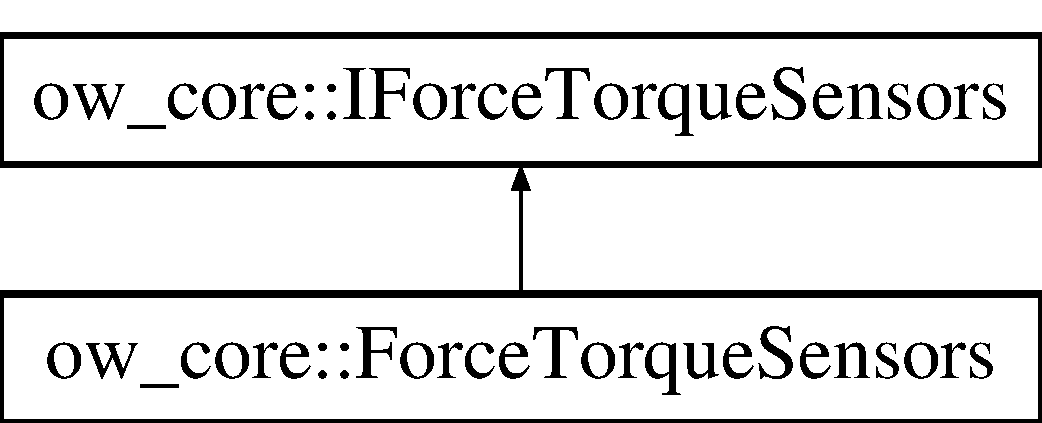
\includegraphics[height=2.000000cm]{dc/da2/classow__core_1_1IForceTorqueSensors}
\end{center}
\end{figure}
\subsection*{Public Member Functions}
\begin{DoxyCompactItemize}
\item 
virtual \hyperlink{classow__core_1_1IForceTorqueSensors_a5b8464f5654189aca50e83b0bb7b6691}{$\sim$\+I\+Force\+Torque\+Sensors} ()\hypertarget{classow__core_1_1IForceTorqueSensors_a5b8464f5654189aca50e83b0bb7b6691}{}\label{classow__core_1_1IForceTorqueSensors_a5b8464f5654189aca50e83b0bb7b6691}

\begin{DoxyCompactList}\small\item\em Virtual destructor. \end{DoxyCompactList}\item 
virtual \hyperlink{classow__core_1_1Wrench}{ow\+::\+Wrench} \& {\bfseries left\+Foot} ()=0\hypertarget{classow__core_1_1IForceTorqueSensors_af653630db1ff0b80c86175f056bced30}{}\label{classow__core_1_1IForceTorqueSensors_af653630db1ff0b80c86175f056bced30}

\item 
virtual const \hyperlink{classow__core_1_1Wrench}{ow\+::\+Wrench} \& {\bfseries left\+Foot} () const =0\hypertarget{classow__core_1_1IForceTorqueSensors_a6f9d3ac17d105ea6a6757d6234fd6b32}{}\label{classow__core_1_1IForceTorqueSensors_a6f9d3ac17d105ea6a6757d6234fd6b32}

\item 
virtual \hyperlink{classow__core_1_1Wrench}{ow\+::\+Wrench} \& {\bfseries right\+Foot} ()=0\hypertarget{classow__core_1_1IForceTorqueSensors_a84f4368356a72384774518a088081390}{}\label{classow__core_1_1IForceTorqueSensors_a84f4368356a72384774518a088081390}

\item 
virtual const \hyperlink{classow__core_1_1Wrench}{ow\+::\+Wrench} \& {\bfseries right\+Foot} () const =0\hypertarget{classow__core_1_1IForceTorqueSensors_a83cb0dd072bc3b05c253ca48fb78311f}{}\label{classow__core_1_1IForceTorqueSensors_a83cb0dd072bc3b05c253ca48fb78311f}

\end{DoxyCompactItemize}


\subsection{Detailed Description}
The \hyperlink{classow__core_1_1IForceTorqueSensors}{I\+Force\+Torque\+Sensors} class. 

Interface class. 

The documentation for this class was generated from the following file\+:\begin{DoxyCompactItemize}
\item 
/home/dean/ros/workspaces/ow\+\_\+test\+\_\+ws/src/ow\+\_\+core/include/ow\+\_\+core/\+Interfaces/\hyperlink{i__force__torque__sensors_8h}{i\+\_\+force\+\_\+torque\+\_\+sensors.\+h}\end{DoxyCompactItemize}

\hypertarget{classow__core_1_1IGenericClass}{}\section{ow\+\_\+core\+:\+:I\+Generic\+Class Class Reference}
\label{classow__core_1_1IGenericClass}\index{ow\+\_\+core\+::\+I\+Generic\+Class@{ow\+\_\+core\+::\+I\+Generic\+Class}}


The \hyperlink{classow__core_1_1IGenericClass}{I\+Generic\+Class} class.  




{\ttfamily \#include $<$i\+\_\+generic\+\_\+class.\+h$>$}

Inheritance diagram for ow\+\_\+core\+:\+:I\+Generic\+Class\+:\begin{figure}[H]
\begin{center}
\leavevmode
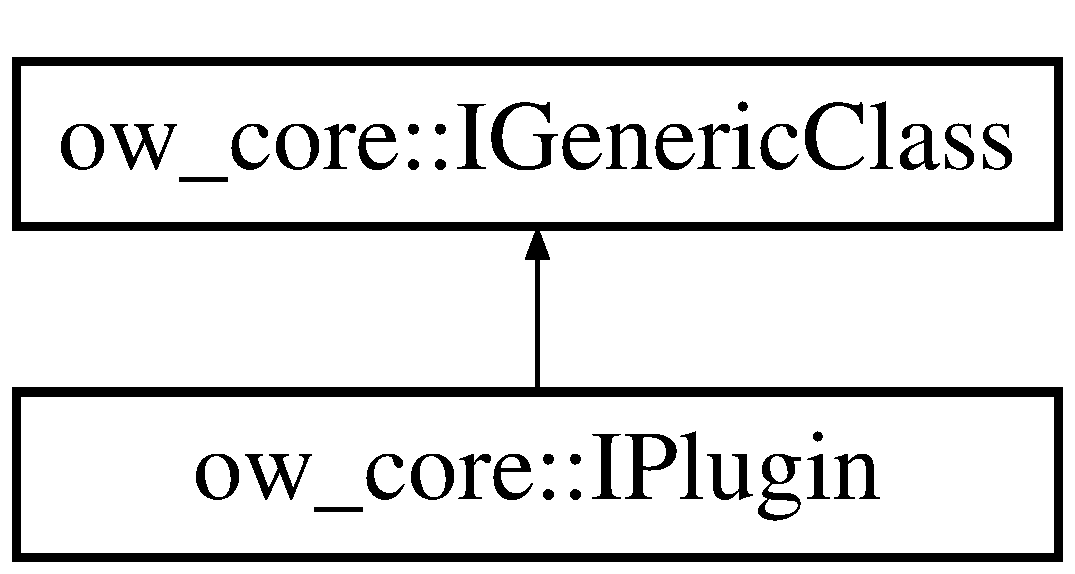
\includegraphics[height=2.000000cm]{da/d72/classow__core_1_1IGenericClass}
\end{center}
\end{figure}
\subsection*{Public Member Functions}
\begin{DoxyCompactItemize}
\item 
virtual \hyperlink{classow__core_1_1IGenericClass_aa0bef13a4de1a0fed78a8e3d3d8a417e}{$\sim$\+I\+Generic\+Class} ()\hypertarget{classow__core_1_1IGenericClass_aa0bef13a4de1a0fed78a8e3d3d8a417e}{}\label{classow__core_1_1IGenericClass_aa0bef13a4de1a0fed78a8e3d3d8a417e}

\begin{DoxyCompactList}\small\item\em Virtual destructor. \end{DoxyCompactList}\item 
virtual std\+::string \hyperlink{classow__core_1_1IGenericClass_ad6ca32fd7189a4bd71c01c10e3677ae4}{class\+Type} () const 
\begin{DoxyCompactList}\small\item\em Get the class type. \end{DoxyCompactList}\end{DoxyCompactItemize}
\subsection*{Static Public Member Functions}
\begin{DoxyCompactItemize}
\item 
static const std\+::string \& \hyperlink{classow__core_1_1IGenericClass_acf2c60d6dde7803ceb855a3f8a3e24b3}{Class\+Type} ()
\begin{DoxyCompactList}\small\item\em The class type of this class. \end{DoxyCompactList}\end{DoxyCompactItemize}


\subsection{Detailed Description}
The \hyperlink{classow__core_1_1IGenericClass}{I\+Generic\+Class} class. 

The interface class for dynamically created classes from a runtime loaded shared library.

N\+O\+TE\+: If you want to create a class dynamically from a runtime loaded shared library, then that class needs to have a virtual destructor.

All Open\+Walker plugins derive from this class to be loadable at runtime. 

\subsection{Member Function Documentation}
\index{ow\+\_\+core\+::\+I\+Generic\+Class@{ow\+\_\+core\+::\+I\+Generic\+Class}!Class\+Type@{Class\+Type}}
\index{Class\+Type@{Class\+Type}!ow\+\_\+core\+::\+I\+Generic\+Class@{ow\+\_\+core\+::\+I\+Generic\+Class}}
\subsubsection[{\texorpdfstring{Class\+Type()}{ClassType()}}]{\setlength{\rightskip}{0pt plus 5cm}static const std\+::string\& ow\+\_\+core\+::\+I\+Generic\+Class\+::\+Class\+Type (
\begin{DoxyParamCaption}
{}
\end{DoxyParamCaption}
)\hspace{0.3cm}{\ttfamily [inline]}, {\ttfamily [static]}}\hypertarget{classow__core_1_1IGenericClass_acf2c60d6dde7803ceb855a3f8a3e24b3}{}\label{classow__core_1_1IGenericClass_acf2c60d6dde7803ceb855a3f8a3e24b3}


The class type of this class. 

Since demangling and mangling are compiler specific we use this function to store the type of a class. This function should be overloaded in all classes that derive from this class. \index{ow\+\_\+core\+::\+I\+Generic\+Class@{ow\+\_\+core\+::\+I\+Generic\+Class}!class\+Type@{class\+Type}}
\index{class\+Type@{class\+Type}!ow\+\_\+core\+::\+I\+Generic\+Class@{ow\+\_\+core\+::\+I\+Generic\+Class}}
\subsubsection[{\texorpdfstring{class\+Type() const }{classType() const }}]{\setlength{\rightskip}{0pt plus 5cm}virtual std\+::string ow\+\_\+core\+::\+I\+Generic\+Class\+::class\+Type (
\begin{DoxyParamCaption}
{}
\end{DoxyParamCaption}
) const\hspace{0.3cm}{\ttfamily [inline]}, {\ttfamily [virtual]}}\hypertarget{classow__core_1_1IGenericClass_ad6ca32fd7189a4bd71c01c10e3677ae4}{}\label{classow__core_1_1IGenericClass_ad6ca32fd7189a4bd71c01c10e3677ae4}


Get the class type. 

Note\+: This identifier can be used to determine the class that this interface abstracts. Then the pointer of this class can be up casted to the correct type.

Note\+: This function should be overwritten by all classes that derive from this class. 

Reimplemented in \hyperlink{classow__core_1_1IPlugin_aff710e9ec9633592c7f013b9c85a4722}{ow\+\_\+core\+::\+I\+Plugin}.



The documentation for this class was generated from the following file\+:\begin{DoxyCompactItemize}
\item 
/home/dean/ros/workspaces/ow\+\_\+test\+\_\+ws/src/ow\+\_\+core/include/ow\+\_\+core/\+Plugins/\hyperlink{i__generic__class_8h}{i\+\_\+generic\+\_\+class.\+h}\end{DoxyCompactItemize}

\hypertarget{classow__core_1_1IImuSensor}{}\section{ow\+\_\+core\+:\+:I\+Imu\+Sensor Class Reference}
\label{classow__core_1_1IImuSensor}\index{ow\+\_\+core\+::\+I\+Imu\+Sensor@{ow\+\_\+core\+::\+I\+Imu\+Sensor}}


The \hyperlink{classow__core_1_1IImuSensor}{I\+Imu\+Sensor} class.  




{\ttfamily \#include $<$i\+\_\+imu\+\_\+sensor.\+h$>$}

Inheritance diagram for ow\+\_\+core\+:\+:I\+Imu\+Sensor\+:\begin{figure}[H]
\begin{center}
\leavevmode
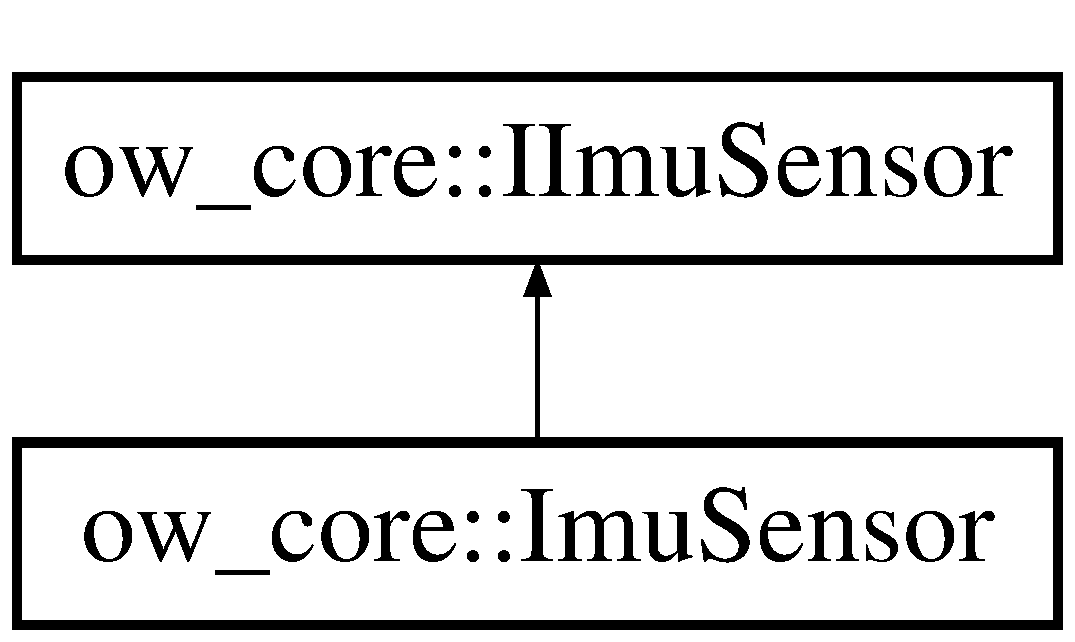
\includegraphics[height=2.000000cm]{dc/dc5/classow__core_1_1IImuSensor}
\end{center}
\end{figure}
\subsection*{Public Member Functions}
\begin{DoxyCompactItemize}
\item 
virtual \hyperlink{classow__core_1_1IImuSensor_adf850e4311f4f949b64052bad6dabaa8}{$\sim$\+I\+Imu\+Sensor} ()\hypertarget{classow__core_1_1IImuSensor_adf850e4311f4f949b64052bad6dabaa8}{}\label{classow__core_1_1IImuSensor_adf850e4311f4f949b64052bad6dabaa8}

\begin{DoxyCompactList}\small\item\em Virtual destructor. \end{DoxyCompactList}\item 
virtual \hyperlink{classow__core_1_1LinearAcceleration}{ow\+::\+Linear\+Acceleration} \& {\bfseries x\+PP} ()=0\hypertarget{classow__core_1_1IImuSensor_ae68fcb47b685e976a9f0d219e4da6161}{}\label{classow__core_1_1IImuSensor_ae68fcb47b685e976a9f0d219e4da6161}

\item 
virtual const \hyperlink{classow__core_1_1LinearAcceleration}{ow\+::\+Linear\+Acceleration} \& {\bfseries x\+PP} () const =0\hypertarget{classow__core_1_1IImuSensor_afa23e2e8bc955e1684838a5702084e69}{}\label{classow__core_1_1IImuSensor_afa23e2e8bc955e1684838a5702084e69}

\item 
virtual \hyperlink{classow__core_1_1AngularPosition}{ow\+::\+Angular\+Position} \& {\bfseries Q} ()=0\hypertarget{classow__core_1_1IImuSensor_a33f9c0749e9b51a160f3e9f7d994a3cf}{}\label{classow__core_1_1IImuSensor_a33f9c0749e9b51a160f3e9f7d994a3cf}

\item 
virtual const \hyperlink{classow__core_1_1AngularPosition}{ow\+::\+Angular\+Position} \& {\bfseries Q} () const =0\hypertarget{classow__core_1_1IImuSensor_a259e35ca45ee2f2f53f87131c4ebb43e}{}\label{classow__core_1_1IImuSensor_a259e35ca45ee2f2f53f87131c4ebb43e}

\item 
virtual \hyperlink{classow__core_1_1AngularVelocity}{ow\+::\+Angular\+Velocity} \& {\bfseries omega} ()=0\hypertarget{classow__core_1_1IImuSensor_ac64f3738634e3d481adeb4d6b136e770}{}\label{classow__core_1_1IImuSensor_ac64f3738634e3d481adeb4d6b136e770}

\item 
virtual const \hyperlink{classow__core_1_1AngularVelocity}{ow\+::\+Angular\+Velocity} \& {\bfseries omega} () const =0\hypertarget{classow__core_1_1IImuSensor_a001199e72daea895d5d27ad408075c28}{}\label{classow__core_1_1IImuSensor_a001199e72daea895d5d27ad408075c28}

\end{DoxyCompactItemize}


\subsection{Detailed Description}
The \hyperlink{classow__core_1_1IImuSensor}{I\+Imu\+Sensor} class. 

Interface class. 

The documentation for this class was generated from the following file\+:\begin{DoxyCompactItemize}
\item 
/home/dean/ros/workspaces/ow\+\_\+test\+\_\+ws/src/ow\+\_\+core/include/ow\+\_\+core/\+Interfaces/\hyperlink{i__imu__sensor_8h}{i\+\_\+imu\+\_\+sensor.\+h}\end{DoxyCompactItemize}

\hypertarget{classow__core_1_1IJoints}{}\section{ow\+\_\+core\+:\+:I\+Joints Class Reference}
\label{classow__core_1_1IJoints}\index{ow\+\_\+core\+::\+I\+Joints@{ow\+\_\+core\+::\+I\+Joints}}


The \hyperlink{classow__core_1_1IJoints}{I\+Joints} class.  




{\ttfamily \#include $<$i\+\_\+joints.\+h$>$}

Inheritance diagram for ow\+\_\+core\+:\+:I\+Joints\+:\begin{figure}[H]
\begin{center}
\leavevmode
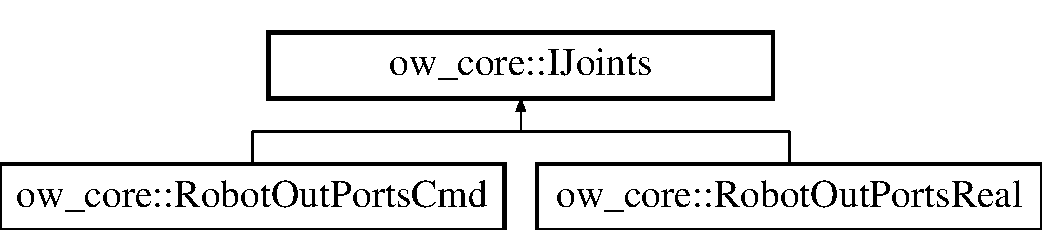
\includegraphics[height=2.000000cm]{dc/db6/classow__core_1_1IJoints}
\end{center}
\end{figure}
\subsection*{Public Member Functions}
\begin{DoxyCompactItemize}
\item 
virtual \hyperlink{classow__core_1_1IJoints_a576ca1a377472f5aad2a9dcc42da9f67}{$\sim$\+I\+Joints} ()\hypertarget{classow__core_1_1IJoints_a576ca1a377472f5aad2a9dcc42da9f67}{}\label{classow__core_1_1IJoints_a576ca1a377472f5aad2a9dcc42da9f67}

\begin{DoxyCompactList}\small\item\em Virtual destructor. \end{DoxyCompactList}\item 
virtual \hyperlink{classow__core_1_1JointState}{ow\+::\+Joint\+State} \& {\bfseries joint\+State} ()=0\hypertarget{classow__core_1_1IJoints_a1429bd69615f934f10bd0d8915275a0a}{}\label{classow__core_1_1IJoints_a1429bd69615f934f10bd0d8915275a0a}

\item 
virtual const \hyperlink{classow__core_1_1JointState}{ow\+::\+Joint\+State} \& {\bfseries joint\+State} () const =0\hypertarget{classow__core_1_1IJoints_ac9e72e3a6f8096b341591ba364a01f08}{}\label{classow__core_1_1IJoints_ac9e72e3a6f8096b341591ba364a01f08}

\end{DoxyCompactItemize}


\subsection{Detailed Description}
The \hyperlink{classow__core_1_1IJoints}{I\+Joints} class. 

Interface class. 

The documentation for this class was generated from the following file\+:\begin{DoxyCompactItemize}
\item 
/home/dean/ros/workspaces/ow\+\_\+test\+\_\+ws/src/ow\+\_\+core/include/ow\+\_\+core/\+Interfaces/\hyperlink{i__joints_8h}{i\+\_\+joints.\+h}\end{DoxyCompactItemize}

\hypertarget{classow__core_1_1ImuSensor}{}\section{ow\+\_\+core\+:\+:Imu\+Sensor Class Reference}
\label{classow__core_1_1ImuSensor}\index{ow\+\_\+core\+::\+Imu\+Sensor@{ow\+\_\+core\+::\+Imu\+Sensor}}


The \hyperlink{classow__core_1_1ImuSensor}{Imu\+Sensor} class.  




{\ttfamily \#include $<$imu\+\_\+sensor.\+h$>$}

Inheritance diagram for ow\+\_\+core\+:\+:Imu\+Sensor\+:\begin{figure}[H]
\begin{center}
\leavevmode
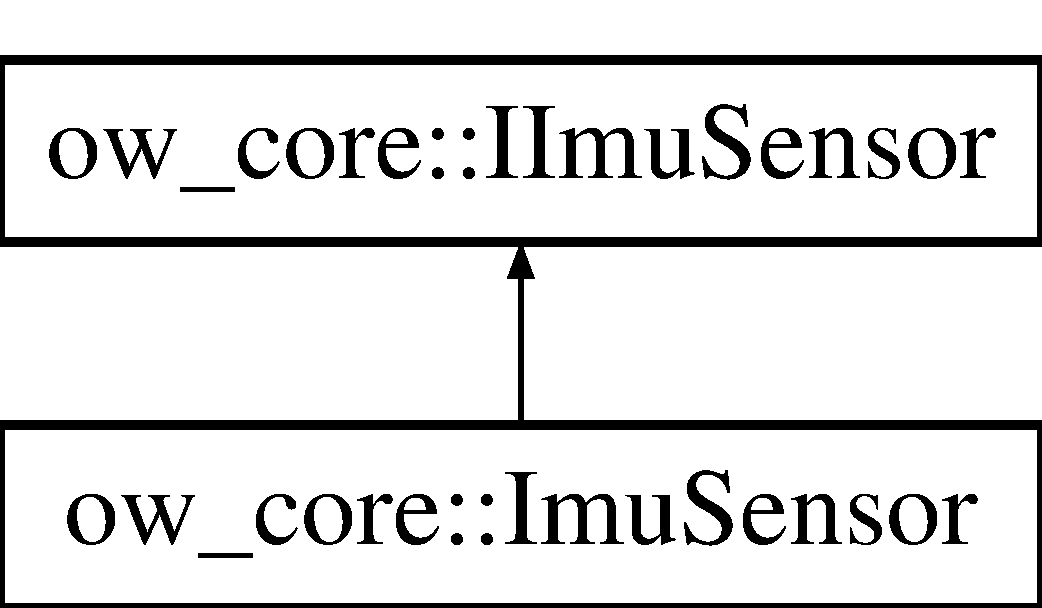
\includegraphics[height=2.000000cm]{d7/d10/classow__core_1_1ImuSensor}
\end{center}
\end{figure}
\subsection*{Public Member Functions}
\begin{DoxyCompactItemize}
\item 
virtual \hyperlink{classow__core_1_1ImuSensor_a55b5d5c2eae34935895d795b0a52b2f4}{$\sim$\+Imu\+Sensor} ()\hypertarget{classow__core_1_1ImuSensor_a55b5d5c2eae34935895d795b0a52b2f4}{}\label{classow__core_1_1ImuSensor_a55b5d5c2eae34935895d795b0a52b2f4}

\begin{DoxyCompactList}\small\item\em Virtual destructor. \end{DoxyCompactList}\item 
virtual \hyperlink{classow__core_1_1LinearAcceleration}{ow\+::\+Linear\+Acceleration} \& {\bfseries x\+PP} ()\hypertarget{classow__core_1_1ImuSensor_a87e3346cbdc77f088ef65bf195cebbf9}{}\label{classow__core_1_1ImuSensor_a87e3346cbdc77f088ef65bf195cebbf9}

\item 
virtual const \hyperlink{classow__core_1_1LinearAcceleration}{ow\+::\+Linear\+Acceleration} \& {\bfseries x\+PP} () const \hypertarget{classow__core_1_1ImuSensor_aee32886eb5a0641d0744604202fb8b94}{}\label{classow__core_1_1ImuSensor_aee32886eb5a0641d0744604202fb8b94}

\item 
virtual \hyperlink{classow__core_1_1AngularPosition}{ow\+::\+Angular\+Position} \& {\bfseries Q} ()\hypertarget{classow__core_1_1ImuSensor_a61e9b747b8e5afc8f68430b832398f52}{}\label{classow__core_1_1ImuSensor_a61e9b747b8e5afc8f68430b832398f52}

\item 
virtual const \hyperlink{classow__core_1_1AngularPosition}{ow\+::\+Angular\+Position} \& {\bfseries Q} () const \hypertarget{classow__core_1_1ImuSensor_a13a6959acd7c32de7455f5494bd5b901}{}\label{classow__core_1_1ImuSensor_a13a6959acd7c32de7455f5494bd5b901}

\item 
virtual \hyperlink{classow__core_1_1AngularVelocity}{ow\+::\+Angular\+Velocity} \& {\bfseries omega} ()\hypertarget{classow__core_1_1ImuSensor_a5db93b43211a8175a07dd35a5fc02cd8}{}\label{classow__core_1_1ImuSensor_a5db93b43211a8175a07dd35a5fc02cd8}

\item 
virtual const \hyperlink{classow__core_1_1AngularVelocity}{ow\+::\+Angular\+Velocity} \& {\bfseries omega} () const \hypertarget{classow__core_1_1ImuSensor_af8c0d8a68476139c42a34b4a13d03ce0}{}\label{classow__core_1_1ImuSensor_af8c0d8a68476139c42a34b4a13d03ce0}

\end{DoxyCompactItemize}
\subsection*{Protected Attributes}
\begin{DoxyCompactItemize}
\item 
\hyperlink{classow__core_1_1LinearAcceleration}{ow\+::\+Linear\+Acceleration} {\bfseries x\+P\+P\+\_\+}\hypertarget{classow__core_1_1ImuSensor_a041ff957f92683213fdcee00fe94fd3e}{}\label{classow__core_1_1ImuSensor_a041ff957f92683213fdcee00fe94fd3e}

\item 
\hyperlink{classow__core_1_1AngularPosition}{ow\+::\+Angular\+Position} {\bfseries Q\+\_\+}\hypertarget{classow__core_1_1ImuSensor_a7cf3f7fdc802c0c8838ac04418ea60b6}{}\label{classow__core_1_1ImuSensor_a7cf3f7fdc802c0c8838ac04418ea60b6}

\item 
\hyperlink{classow__core_1_1AngularVelocity}{ow\+::\+Angular\+Velocity} {\bfseries omega\+\_\+}\hypertarget{classow__core_1_1ImuSensor_a5c3e1f8c791bf7118cdf30bd552b60c7}{}\label{classow__core_1_1ImuSensor_a5c3e1f8c791bf7118cdf30bd552b60c7}

\end{DoxyCompactItemize}


\subsection{Detailed Description}
The \hyperlink{classow__core_1_1ImuSensor}{Imu\+Sensor} class. 

The default implementation of the \hyperlink{classow__core_1_1IImuSensor}{I\+Imu\+Sensor} interface. 

The documentation for this class was generated from the following file\+:\begin{DoxyCompactItemize}
\item 
/home/dean/ros/workspaces/ow\+\_\+test\+\_\+ws/src/ow\+\_\+core/include/ow\+\_\+core/\+Implementations/\hyperlink{imu__sensor_8h}{imu\+\_\+sensor.\+h}\end{DoxyCompactItemize}

\hypertarget{classow__core_1_1IPlugin}{}\section{ow\+\_\+core\+:\+:I\+Plugin Class Reference}
\label{classow__core_1_1IPlugin}\index{ow\+\_\+core\+::\+I\+Plugin@{ow\+\_\+core\+::\+I\+Plugin}}


The \hyperlink{classow__core_1_1IPlugin}{I\+Plugin} class.  




{\ttfamily \#include $<$i\+\_\+plugin.\+h$>$}

Inheritance diagram for ow\+\_\+core\+:\+:I\+Plugin\+:\begin{figure}[H]
\begin{center}
\leavevmode
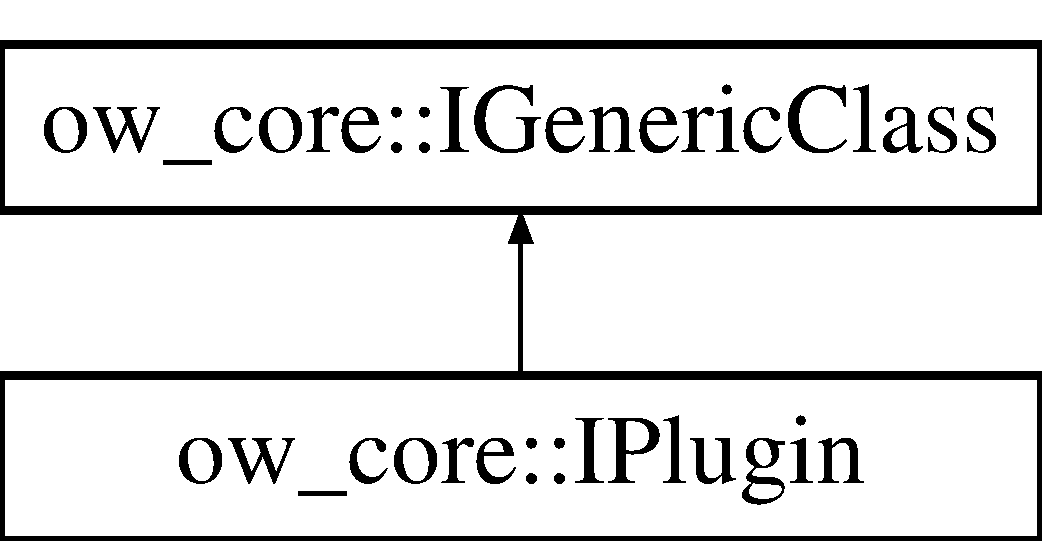
\includegraphics[height=2.000000cm]{d7/d66/classow__core_1_1IPlugin}
\end{center}
\end{figure}
\subsection*{Public Member Functions}
\begin{DoxyCompactItemize}
\item 
virtual \hyperlink{classow__core_1_1IPlugin_a90c54611f7b8bf246676cd7f19077053}{$\sim$\+I\+Plugin} ()\hypertarget{classow__core_1_1IPlugin_a90c54611f7b8bf246676cd7f19077053}{}\label{classow__core_1_1IPlugin_a90c54611f7b8bf246676cd7f19077053}

\begin{DoxyCompactList}\small\item\em Virtual destructor. \end{DoxyCompactList}\item 
virtual std\+::string \hyperlink{classow__core_1_1IPlugin_aff710e9ec9633592c7f013b9c85a4722}{class\+Type} () const 
\begin{DoxyCompactList}\small\item\em Get the class type. \end{DoxyCompactList}\end{DoxyCompactItemize}
\subsection*{Static Public Member Functions}
\begin{DoxyCompactItemize}
\item 
static const std\+::string \& \hyperlink{classow__core_1_1IPlugin_a55979a29b69adc98803cc6eff1f91f89}{Class\+Type} ()
\begin{DoxyCompactList}\small\item\em The class type of this class. \end{DoxyCompactList}\end{DoxyCompactItemize}


\subsection{Detailed Description}
The \hyperlink{classow__core_1_1IPlugin}{I\+Plugin} class. 

This is the base class for all Open\+Walker plugins. 

\subsection{Member Function Documentation}
\index{ow\+\_\+core\+::\+I\+Plugin@{ow\+\_\+core\+::\+I\+Plugin}!Class\+Type@{Class\+Type}}
\index{Class\+Type@{Class\+Type}!ow\+\_\+core\+::\+I\+Plugin@{ow\+\_\+core\+::\+I\+Plugin}}
\subsubsection[{\texorpdfstring{Class\+Type()}{ClassType()}}]{\setlength{\rightskip}{0pt plus 5cm}static const std\+::string\& ow\+\_\+core\+::\+I\+Plugin\+::\+Class\+Type (
\begin{DoxyParamCaption}
{}
\end{DoxyParamCaption}
)\hspace{0.3cm}{\ttfamily [inline]}, {\ttfamily [static]}}\hypertarget{classow__core_1_1IPlugin_a55979a29b69adc98803cc6eff1f91f89}{}\label{classow__core_1_1IPlugin_a55979a29b69adc98803cc6eff1f91f89}


The class type of this class. 

Since demangling and mangling are compiler specific we use this function to store the type of a class. This function should be overloaded in all classes that derive from this class. \index{ow\+\_\+core\+::\+I\+Plugin@{ow\+\_\+core\+::\+I\+Plugin}!class\+Type@{class\+Type}}
\index{class\+Type@{class\+Type}!ow\+\_\+core\+::\+I\+Plugin@{ow\+\_\+core\+::\+I\+Plugin}}
\subsubsection[{\texorpdfstring{class\+Type() const }{classType() const }}]{\setlength{\rightskip}{0pt plus 5cm}virtual std\+::string ow\+\_\+core\+::\+I\+Plugin\+::class\+Type (
\begin{DoxyParamCaption}
{}
\end{DoxyParamCaption}
) const\hspace{0.3cm}{\ttfamily [inline]}, {\ttfamily [virtual]}}\hypertarget{classow__core_1_1IPlugin_aff710e9ec9633592c7f013b9c85a4722}{}\label{classow__core_1_1IPlugin_aff710e9ec9633592c7f013b9c85a4722}


Get the class type. 

Note\+: This identifier can be used to determine the class that this interface abstracts. Then the pointer of this class can be up casted to the correct type.

Note\+: This function should be overwritten by all classes that derive from this class. 

Reimplemented from \hyperlink{classow__core_1_1IGenericClass_ad6ca32fd7189a4bd71c01c10e3677ae4}{ow\+\_\+core\+::\+I\+Generic\+Class}.



The documentation for this class was generated from the following file\+:\begin{DoxyCompactItemize}
\item 
/home/dean/ros/workspaces/ow\+\_\+test\+\_\+ws/src/ow\+\_\+core/include/ow\+\_\+core/\+Plugins/\hyperlink{i__plugin_8h}{i\+\_\+plugin.\+h}\end{DoxyCompactItemize}

\hypertarget{classow__core_1_1IRobot}{}\section{ow\+\_\+core\+:\+:I\+Robot Class Reference}
\label{classow__core_1_1IRobot}\index{ow\+\_\+core\+::\+I\+Robot@{ow\+\_\+core\+::\+I\+Robot}}


The \hyperlink{classow__core_1_1IRobot}{I\+Robot} class.  




{\ttfamily \#include $<$i\+\_\+robot.\+h$>$}

\subsection*{Public Member Functions}
\begin{DoxyCompactItemize}
\item 
virtual \hyperlink{classow__core_1_1IRobot_a22760209db12499291efb200e906ed3c}{$\sim$\+I\+Robot} ()\hypertarget{classow__core_1_1IRobot_a22760209db12499291efb200e906ed3c}{}\label{classow__core_1_1IRobot_a22760209db12499291efb200e906ed3c}

\begin{DoxyCompactList}\small\item\em Virtual destructor. \end{DoxyCompactList}\item 
virtual \hyperlink{classow__core_1_1IRobot_a9bdff9f15015cda18554c4dddf728928}{connect\+In\+Port} (const I\+Inverse\+Kinematics\+Out\+Ports $\ast$ik)=0
\begin{DoxyCompactList}\small\item\em Connect to in port. \end{DoxyCompactList}\item 
virtual const \hyperlink{classow__core_1_1IRobotOutPorts}{I\+Robot\+Out\+Ports} $\ast$ {\bfseries out\+Ports} () const =0\hypertarget{classow__core_1_1IRobot_a50f7cf4bb874717667bd03d3bdac7c80}{}\label{classow__core_1_1IRobot_a50f7cf4bb874717667bd03d3bdac7c80}

\end{DoxyCompactItemize}


\subsection{Detailed Description}
The \hyperlink{classow__core_1_1IRobot}{I\+Robot} class. 

Interface class.

\begin{DoxyRefDesc}{Todo}
\item[\hyperlink{todo__todo000011}{Todo}]Remove forward declaration of I\+Inverse\+Kinematics\+Out\+Ports. \end{DoxyRefDesc}


\subsection{Member Function Documentation}
\index{ow\+\_\+core\+::\+I\+Robot@{ow\+\_\+core\+::\+I\+Robot}!connect\+In\+Port@{connect\+In\+Port}}
\index{connect\+In\+Port@{connect\+In\+Port}!ow\+\_\+core\+::\+I\+Robot@{ow\+\_\+core\+::\+I\+Robot}}
\subsubsection[{\texorpdfstring{connect\+In\+Port(const I\+Inverse\+Kinematics\+Out\+Ports $\ast$ik)=0}{connectInPort(const IInverseKinematicsOutPorts *ik)=0}}]{\setlength{\rightskip}{0pt plus 5cm}virtual ow\+\_\+core\+::\+I\+Robot\+::connect\+In\+Port (
\begin{DoxyParamCaption}
\item[{const I\+Inverse\+Kinematics\+Out\+Ports $\ast$}]{ik}
\end{DoxyParamCaption}
)\hspace{0.3cm}{\ttfamily [pure virtual]}}\hypertarget{classow__core_1_1IRobot_a9bdff9f15015cda18554c4dddf728928}{}\label{classow__core_1_1IRobot_a9bdff9f15015cda18554c4dddf728928}


Connect to in port. 

Connects this module to the out port of another module.

N\+O\+TE\+: The pointer is constant. This module reads only the out port of the other module. 

The documentation for this class was generated from the following file\+:\begin{DoxyCompactItemize}
\item 
/home/dean/ros/workspaces/ow\+\_\+test\+\_\+ws/src/ow\+\_\+core/include/ow\+\_\+core/\+Interfaces/\hyperlink{i__robot_8h}{i\+\_\+robot.\+h}\end{DoxyCompactItemize}

\hypertarget{classow__core_1_1IRobotOutPorts}{}\section{ow\+\_\+core\+:\+:I\+Robot\+Out\+Ports Class Reference}
\label{classow__core_1_1IRobotOutPorts}\index{ow\+\_\+core\+::\+I\+Robot\+Out\+Ports@{ow\+\_\+core\+::\+I\+Robot\+Out\+Ports}}


The \hyperlink{classow__core_1_1IRobotOutPorts}{I\+Robot\+Out\+Ports} class.  




{\ttfamily \#include $<$i\+\_\+robot\+\_\+out\+\_\+ports.\+h$>$}

Inheritance diagram for ow\+\_\+core\+:\+:I\+Robot\+Out\+Ports\+:\begin{figure}[H]
\begin{center}
\leavevmode
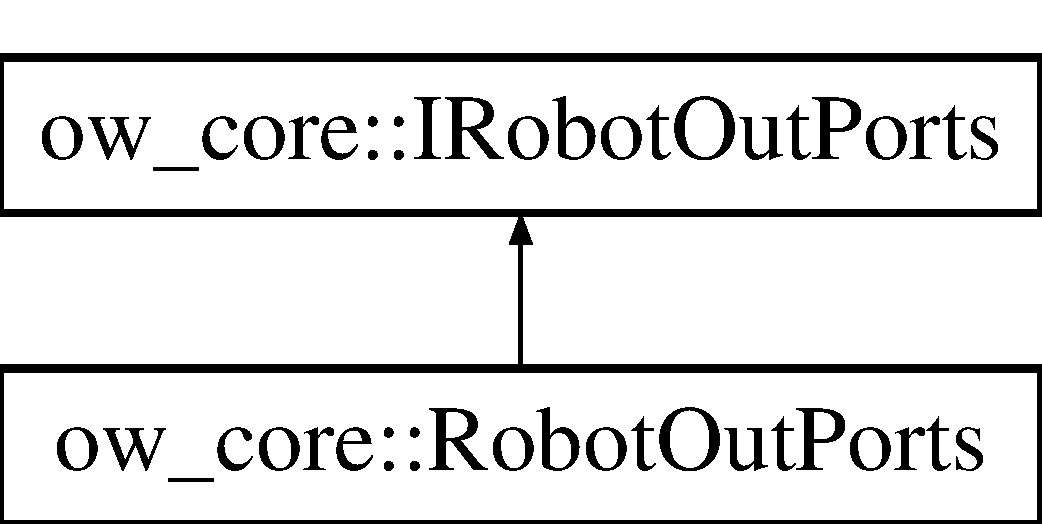
\includegraphics[height=2.000000cm]{d2/d40/classow__core_1_1IRobotOutPorts}
\end{center}
\end{figure}
\subsection*{Public Member Functions}
\begin{DoxyCompactItemize}
\item 
virtual \hyperlink{classow__core_1_1IRobotOutPorts_a9bbe52128f66b50c0b9b3859abbdebaa}{$\sim$\+I\+Robot\+Out\+Ports} ()\hypertarget{classow__core_1_1IRobotOutPorts_a9bbe52128f66b50c0b9b3859abbdebaa}{}\label{classow__core_1_1IRobotOutPorts_a9bbe52128f66b50c0b9b3859abbdebaa}

\begin{DoxyCompactList}\small\item\em Virtual destructor. \end{DoxyCompactList}\item 
virtual \hyperlink{classow__core_1_1IRobotOutPortsReal}{I\+Robot\+Out\+Ports\+Real} $\ast$ {\bfseries real} ()=0\hypertarget{classow__core_1_1IRobotOutPorts_a79a79d009b41a67c6b471e3d4d57d341}{}\label{classow__core_1_1IRobotOutPorts_a79a79d009b41a67c6b471e3d4d57d341}

\item 
virtual const \hyperlink{classow__core_1_1IRobotOutPortsReal}{I\+Robot\+Out\+Ports\+Real} $\ast$ {\bfseries real} () const =0\hypertarget{classow__core_1_1IRobotOutPorts_af5d9270760417b332147e9239094b595}{}\label{classow__core_1_1IRobotOutPorts_af5d9270760417b332147e9239094b595}

\item 
virtual \hyperlink{classow__core_1_1IRobotOutPortsCmd}{I\+Robot\+Out\+Ports\+Cmd} $\ast$ {\bfseries cmd} ()=0\hypertarget{classow__core_1_1IRobotOutPorts_a876b27868b7bd548aec6823820dbb37a}{}\label{classow__core_1_1IRobotOutPorts_a876b27868b7bd548aec6823820dbb37a}

\item 
virtual const \hyperlink{classow__core_1_1IRobotOutPortsCmd}{I\+Robot\+Out\+Ports\+Cmd} $\ast$ {\bfseries cmd} () const =0\hypertarget{classow__core_1_1IRobotOutPorts_ac086ad94f86fcb4c7eb16dc2daeef96d}{}\label{classow__core_1_1IRobotOutPorts_ac086ad94f86fcb4c7eb16dc2daeef96d}

\end{DoxyCompactItemize}


\subsection{Detailed Description}
The \hyperlink{classow__core_1_1IRobotOutPorts}{I\+Robot\+Out\+Ports} class. 

Interface class. 

The documentation for this class was generated from the following file\+:\begin{DoxyCompactItemize}
\item 
/home/dean/ros/workspaces/ow\+\_\+test\+\_\+ws/src/ow\+\_\+core/include/ow\+\_\+core/\+Interfaces/\hyperlink{i__robot__out__ports_8h}{i\+\_\+robot\+\_\+out\+\_\+ports.\+h}\end{DoxyCompactItemize}

\hypertarget{classow__core_1_1IRobotOutPortsCmd}{}\section{ow\+\_\+core\+:\+:I\+Robot\+Out\+Ports\+Cmd Class Reference}
\label{classow__core_1_1IRobotOutPortsCmd}\index{ow\+\_\+core\+::\+I\+Robot\+Out\+Ports\+Cmd@{ow\+\_\+core\+::\+I\+Robot\+Out\+Ports\+Cmd}}


The \hyperlink{classow__core_1_1IRobotOutPortsCmd}{I\+Robot\+Out\+Ports\+Cmd} class.  




{\ttfamily \#include $<$i\+\_\+robot\+\_\+out\+\_\+ports\+\_\+cmd.\+h$>$}

Inheritance diagram for ow\+\_\+core\+:\+:I\+Robot\+Out\+Ports\+Cmd\+:\begin{figure}[H]
\begin{center}
\leavevmode
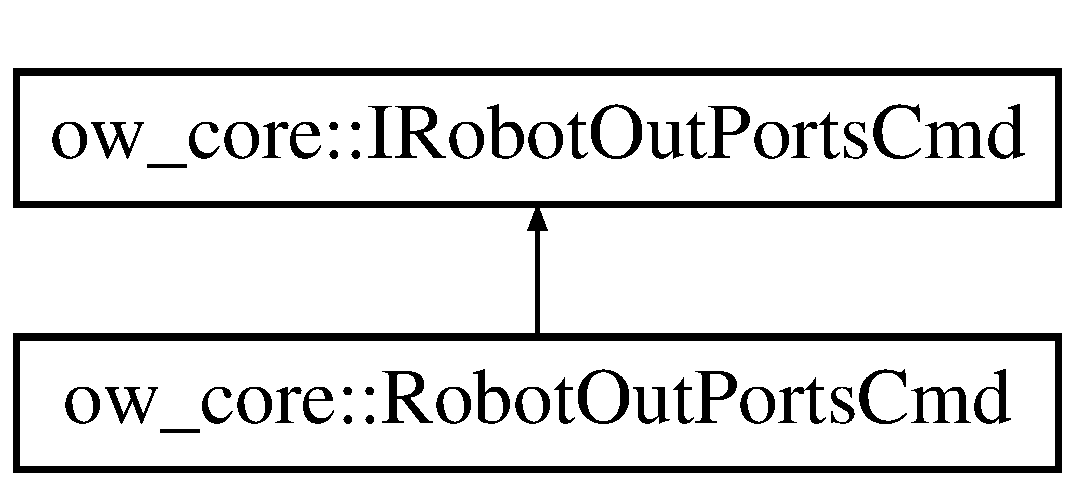
\includegraphics[height=2.000000cm]{d9/dce/classow__core_1_1IRobotOutPortsCmd}
\end{center}
\end{figure}
\subsection*{Public Member Functions}
\begin{DoxyCompactItemize}
\item 
virtual \hyperlink{classow__core_1_1IRobotOutPortsCmd_a33b6764ab04df38260bd20680aea1500}{$\sim$\+I\+Robot\+Out\+Ports\+Cmd} ()\hypertarget{classow__core_1_1IRobotOutPortsCmd_a33b6764ab04df38260bd20680aea1500}{}\label{classow__core_1_1IRobotOutPortsCmd_a33b6764ab04df38260bd20680aea1500}

\begin{DoxyCompactList}\small\item\em Virtual destructor. \end{DoxyCompactList}\item 
virtual \hyperlink{classow__core_1_1IJoints}{I\+Joints} $\ast$ {\bfseries joints} ()=0\hypertarget{classow__core_1_1IRobotOutPortsCmd_a4285bd03e22215bb48c255d14d322255}{}\label{classow__core_1_1IRobotOutPortsCmd_a4285bd03e22215bb48c255d14d322255}

\item 
virtual const \hyperlink{classow__core_1_1IJoints}{I\+Joints} $\ast$ {\bfseries joints} () const =0\hypertarget{classow__core_1_1IRobotOutPortsCmd_a08ce418625a9680ae6c2e00efb2a2119}{}\label{classow__core_1_1IRobotOutPortsCmd_a08ce418625a9680ae6c2e00efb2a2119}

\end{DoxyCompactItemize}


\subsection{Detailed Description}
The \hyperlink{classow__core_1_1IRobotOutPortsCmd}{I\+Robot\+Out\+Ports\+Cmd} class. 

Interface class. 

The documentation for this class was generated from the following file\+:\begin{DoxyCompactItemize}
\item 
/home/dean/ros/workspaces/ow\+\_\+test\+\_\+ws/src/ow\+\_\+core/include/ow\+\_\+core/\+Interfaces/\hyperlink{i__robot__out__ports__cmd_8h}{i\+\_\+robot\+\_\+out\+\_\+ports\+\_\+cmd.\+h}\end{DoxyCompactItemize}

\hypertarget{classow__core_1_1IRobotOutPortsReal}{}\section{ow\+\_\+core\+:\+:I\+Robot\+Out\+Ports\+Real Class Reference}
\label{classow__core_1_1IRobotOutPortsReal}\index{ow\+\_\+core\+::\+I\+Robot\+Out\+Ports\+Real@{ow\+\_\+core\+::\+I\+Robot\+Out\+Ports\+Real}}


The \hyperlink{classow__core_1_1IRobotOutPortsReal}{I\+Robot\+Out\+Ports\+Real} class.  




{\ttfamily \#include $<$i\+\_\+robot\+\_\+out\+\_\+ports\+\_\+real.\+h$>$}

Inheritance diagram for ow\+\_\+core\+:\+:I\+Robot\+Out\+Ports\+Real\+:\begin{figure}[H]
\begin{center}
\leavevmode
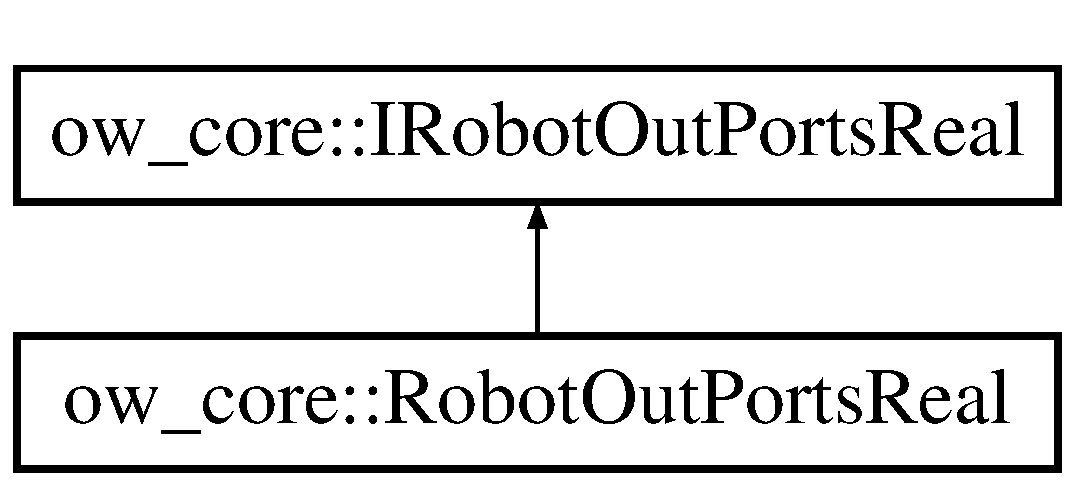
\includegraphics[height=2.000000cm]{d6/d66/classow__core_1_1IRobotOutPortsReal}
\end{center}
\end{figure}
\subsection*{Public Member Functions}
\begin{DoxyCompactItemize}
\item 
virtual \hyperlink{classow__core_1_1IRobotOutPortsReal_a91e455a48af77b20a48216e47dd7a999}{$\sim$\+I\+Robot\+Out\+Ports\+Real} ()\hypertarget{classow__core_1_1IRobotOutPortsReal_a91e455a48af77b20a48216e47dd7a999}{}\label{classow__core_1_1IRobotOutPortsReal_a91e455a48af77b20a48216e47dd7a999}

\begin{DoxyCompactList}\small\item\em Virtual destructor. \end{DoxyCompactList}\item 
virtual \hyperlink{classow__core_1_1IImuSensor}{I\+Imu\+Sensor} $\ast$ {\bfseries imu\+Sensor} ()=0\hypertarget{classow__core_1_1IRobotOutPortsReal_a7ba473ab64924a9aacb0b84d532c4ed5}{}\label{classow__core_1_1IRobotOutPortsReal_a7ba473ab64924a9aacb0b84d532c4ed5}

\item 
virtual const \hyperlink{classow__core_1_1IImuSensor}{I\+Imu\+Sensor} $\ast$ {\bfseries imu\+Sensor} () const =0\hypertarget{classow__core_1_1IRobotOutPortsReal_ab3bd85b21d59a4728e7332f809a6a768}{}\label{classow__core_1_1IRobotOutPortsReal_ab3bd85b21d59a4728e7332f809a6a768}

\item 
virtual \hyperlink{classow__core_1_1IForceTorqueSensors}{I\+Force\+Torque\+Sensors} $\ast$ {\bfseries force\+Torque\+Sensors} ()=0\hypertarget{classow__core_1_1IRobotOutPortsReal_afe1083e36b6b76117495876bddf43001}{}\label{classow__core_1_1IRobotOutPortsReal_afe1083e36b6b76117495876bddf43001}

\item 
virtual const \hyperlink{classow__core_1_1IForceTorqueSensors}{I\+Force\+Torque\+Sensors} $\ast$ {\bfseries force\+Torque\+Sensors} () const =0\hypertarget{classow__core_1_1IRobotOutPortsReal_ad269f5ca4d0d06dcc26dc1049e409326}{}\label{classow__core_1_1IRobotOutPortsReal_ad269f5ca4d0d06dcc26dc1049e409326}

\item 
virtual \hyperlink{classow__core_1_1IJoints}{I\+Joints} $\ast$ {\bfseries joints} ()=0\hypertarget{classow__core_1_1IRobotOutPortsReal_a79db66bcb85982efc66f3aa5d8b34246}{}\label{classow__core_1_1IRobotOutPortsReal_a79db66bcb85982efc66f3aa5d8b34246}

\item 
virtual const \hyperlink{classow__core_1_1IJoints}{I\+Joints} $\ast$ {\bfseries joints} () const =0\hypertarget{classow__core_1_1IRobotOutPortsReal_a7b3523992c44f9207e56776fd56dadaa}{}\label{classow__core_1_1IRobotOutPortsReal_a7b3523992c44f9207e56776fd56dadaa}

\end{DoxyCompactItemize}


\subsection{Detailed Description}
The \hyperlink{classow__core_1_1IRobotOutPortsReal}{I\+Robot\+Out\+Ports\+Real} class. 

Interface class. 

The documentation for this class was generated from the following file\+:\begin{DoxyCompactItemize}
\item 
/home/dean/ros/workspaces/ow\+\_\+test\+\_\+ws/src/ow\+\_\+core/include/ow\+\_\+core/\+Interfaces/\hyperlink{i__robot__out__ports__real_8h}{i\+\_\+robot\+\_\+out\+\_\+ports\+\_\+real.\+h}\end{DoxyCompactItemize}

\hypertarget{classow__core_1_1JointAcceleration}{}\section{ow\+\_\+core\+:\+:Joint\+Acceleration$<$ \+\_\+\+Scalar, \+\_\+\+Rows $>$ Class Template Reference}
\label{classow__core_1_1JointAcceleration}\index{ow\+\_\+core\+::\+Joint\+Acceleration$<$ \+\_\+\+Scalar, \+\_\+\+Rows $>$@{ow\+\_\+core\+::\+Joint\+Acceleration$<$ \+\_\+\+Scalar, \+\_\+\+Rows $>$}}


The \hyperlink{classow__core_1_1JointAcceleration}{Joint\+Acceleration} class.  




{\ttfamily \#include $<$joint\+\_\+acceleration.\+h$>$}

Inheritance diagram for ow\+\_\+core\+:\+:Joint\+Acceleration$<$ \+\_\+\+Scalar, \+\_\+\+Rows $>$\+:\begin{figure}[H]
\begin{center}
\leavevmode
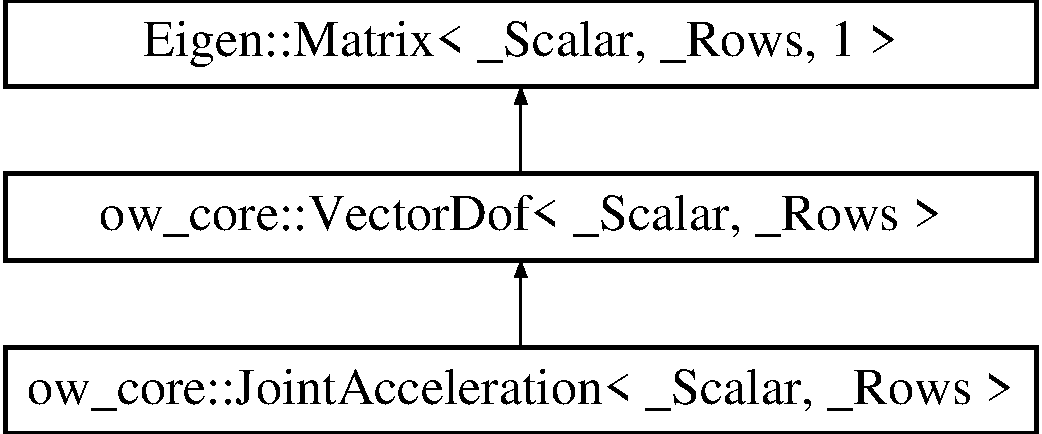
\includegraphics[height=3.000000cm]{d9/d9f/classow__core_1_1JointAcceleration}
\end{center}
\end{figure}
\subsection*{Public Types}
\begin{DoxyCompactItemize}
\item 
enum \{ {\bfseries Rows} = \+\_\+\+Rows
 \}\hypertarget{classow__core_1_1JointAcceleration_a21c841c75e8afcecd1957adc7406524d}{}\label{classow__core_1_1JointAcceleration_a21c841c75e8afcecd1957adc7406524d}

\item 
typedef \+\_\+\+Scalar {\bfseries Scalar}\hypertarget{classow__core_1_1JointAcceleration_a3aef897869dad7025edeffbc67d1bfd9}{}\label{classow__core_1_1JointAcceleration_a3aef897869dad7025edeffbc67d1bfd9}

\item 
typedef \hyperlink{classow__core_1_1VectorDof}{Vector\+Dof}$<$ Scalar, Rows $>$ {\bfseries Base}\hypertarget{classow__core_1_1JointAcceleration_aa9b376c4517796a54f984b190c1c4dcf}{}\label{classow__core_1_1JointAcceleration_aa9b376c4517796a54f984b190c1c4dcf}

\end{DoxyCompactItemize}
\subsection*{Public Member Functions}
\begin{DoxyCompactItemize}
\item 
\hyperlink{classow__core_1_1JointAcceleration_aa5de527dfa135e326e6686fa812b5e83}{Joint\+Acceleration} ()\hypertarget{classow__core_1_1JointAcceleration_aa5de527dfa135e326e6686fa812b5e83}{}\label{classow__core_1_1JointAcceleration_aa5de527dfa135e326e6686fa812b5e83}

\begin{DoxyCompactList}\small\item\em Default Constructor. \end{DoxyCompactList}\item 
{\footnotesize template$<$typename Other\+Derived $>$ }\\\hyperlink{classow__core_1_1JointAcceleration_a84e8c4190777f4f93b7a45f5e0195d5d}{Joint\+Acceleration} (const Eigen\+::\+Eigen\+Base$<$ Other\+Derived $>$ \&other)
\begin{DoxyCompactList}\small\item\em Copy constructor. \end{DoxyCompactList}\end{DoxyCompactItemize}
\subsection*{Additional Inherited Members}


\subsection{Detailed Description}
\subsubsection*{template$<$typename \+\_\+\+Scalar, int \+\_\+\+Rows$>$\\*
class ow\+\_\+core\+::\+Joint\+Acceleration$<$ \+\_\+\+Scalar, \+\_\+\+Rows $>$}

The \hyperlink{classow__core_1_1JointAcceleration}{Joint\+Acceleration} class. 

The \hyperlink{classow__core_1_1JointAcceleration}{Joint\+Acceleration} is of type \hyperlink{classow__core_1_1VectorDof}{Vector\+Dof} and is represented by the math symbol $\mathbf{\ddot{q}}$. 

\subsection{Constructor \& Destructor Documentation}
\index{ow\+\_\+core\+::\+Joint\+Acceleration@{ow\+\_\+core\+::\+Joint\+Acceleration}!Joint\+Acceleration@{Joint\+Acceleration}}
\index{Joint\+Acceleration@{Joint\+Acceleration}!ow\+\_\+core\+::\+Joint\+Acceleration@{ow\+\_\+core\+::\+Joint\+Acceleration}}
\subsubsection[{\texorpdfstring{Joint\+Acceleration(const Eigen\+::\+Eigen\+Base$<$ Other\+Derived $>$ \&other)}{JointAcceleration(const Eigen::EigenBase< OtherDerived > &other)}}]{\setlength{\rightskip}{0pt plus 5cm}template$<$typename \+\_\+\+Scalar, int \+\_\+\+Rows$>$ template$<$typename Other\+Derived $>$ {\bf ow\+\_\+core\+::\+Joint\+Acceleration}$<$ \+\_\+\+Scalar, \+\_\+\+Rows $>$\+::{\bf Joint\+Acceleration} (
\begin{DoxyParamCaption}
\item[{const Eigen\+::\+Eigen\+Base$<$ Other\+Derived $>$ \&}]{other}
\end{DoxyParamCaption}
)\hspace{0.3cm}{\ttfamily [inline]}}\hypertarget{classow__core_1_1JointAcceleration_a84e8c4190777f4f93b7a45f5e0195d5d}{}\label{classow__core_1_1JointAcceleration_a84e8c4190777f4f93b7a45f5e0195d5d}


Copy constructor. 

This copy constructor not only works with Eigen matrices but also with their expressions. 

The documentation for this class was generated from the following file\+:\begin{DoxyCompactItemize}
\item 
/home/dean/ros/workspaces/ow\+\_\+test\+\_\+ws/src/ow\+\_\+core/include/ow\+\_\+core/\hyperlink{joint__acceleration_8h}{joint\+\_\+acceleration.\+h}\end{DoxyCompactItemize}

\hypertarget{classow__core_1_1JointEffort}{}\section{ow\+\_\+core\+:\+:Joint\+Effort$<$ \+\_\+\+Scalar, \+\_\+\+Rows $>$ Class Template Reference}
\label{classow__core_1_1JointEffort}\index{ow\+\_\+core\+::\+Joint\+Effort$<$ \+\_\+\+Scalar, \+\_\+\+Rows $>$@{ow\+\_\+core\+::\+Joint\+Effort$<$ \+\_\+\+Scalar, \+\_\+\+Rows $>$}}


The \hyperlink{classow__core_1_1JointEffort}{Joint\+Effort} class.  




{\ttfamily \#include $<$joint\+\_\+effort.\+h$>$}

Inheritance diagram for ow\+\_\+core\+:\+:Joint\+Effort$<$ \+\_\+\+Scalar, \+\_\+\+Rows $>$\+:\begin{figure}[H]
\begin{center}
\leavevmode
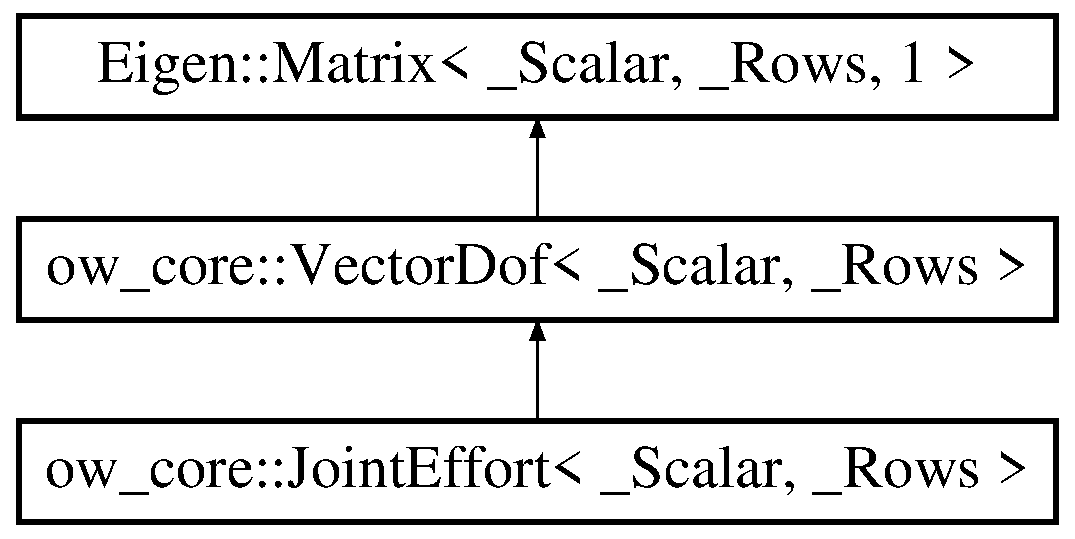
\includegraphics[height=3.000000cm]{d5/d72/classow__core_1_1JointEffort}
\end{center}
\end{figure}
\subsection*{Public Types}
\begin{DoxyCompactItemize}
\item 
enum \{ {\bfseries Rows} = \+\_\+\+Rows
 \}\hypertarget{classow__core_1_1JointEffort_a0f8319255d9cf53d1124a8fd22ea6714}{}\label{classow__core_1_1JointEffort_a0f8319255d9cf53d1124a8fd22ea6714}

\item 
typedef \+\_\+\+Scalar {\bfseries Scalar}\hypertarget{classow__core_1_1JointEffort_a1576c88bb00bbb19d625a30d5ed08b52}{}\label{classow__core_1_1JointEffort_a1576c88bb00bbb19d625a30d5ed08b52}

\item 
typedef \hyperlink{classow__core_1_1VectorDof}{Vector\+Dof}$<$ Scalar, Rows $>$ {\bfseries Base}\hypertarget{classow__core_1_1JointEffort_a90396788f55c3c2bb37536d70153a374}{}\label{classow__core_1_1JointEffort_a90396788f55c3c2bb37536d70153a374}

\end{DoxyCompactItemize}
\subsection*{Public Member Functions}
\begin{DoxyCompactItemize}
\item 
\hyperlink{classow__core_1_1JointEffort_a7a6eb1b97b2b8b3bac294a1c2115b277}{Joint\+Effort} ()\hypertarget{classow__core_1_1JointEffort_a7a6eb1b97b2b8b3bac294a1c2115b277}{}\label{classow__core_1_1JointEffort_a7a6eb1b97b2b8b3bac294a1c2115b277}

\begin{DoxyCompactList}\small\item\em Default Constructor. \end{DoxyCompactList}\item 
{\footnotesize template$<$typename Other\+Derived $>$ }\\\hyperlink{classow__core_1_1JointEffort_ab554628edbca575f0134f5604bedbdec}{Joint\+Effort} (const Eigen\+::\+Eigen\+Base$<$ Other\+Derived $>$ \&other)
\begin{DoxyCompactList}\small\item\em Copy constructor. \end{DoxyCompactList}\end{DoxyCompactItemize}
\subsection*{Additional Inherited Members}


\subsection{Detailed Description}
\subsubsection*{template$<$typename \+\_\+\+Scalar, int \+\_\+\+Rows$>$\\*
class ow\+\_\+core\+::\+Joint\+Effort$<$ \+\_\+\+Scalar, \+\_\+\+Rows $>$}

The \hyperlink{classow__core_1_1JointEffort}{Joint\+Effort} class. 

The \hyperlink{classow__core_1_1JointEffort}{Joint\+Effort} is of type \hyperlink{classow__core_1_1VectorDof}{Vector\+Dof} and is represented by the math symbol $\mathbf{\tau}$. 

\subsection{Constructor \& Destructor Documentation}
\index{ow\+\_\+core\+::\+Joint\+Effort@{ow\+\_\+core\+::\+Joint\+Effort}!Joint\+Effort@{Joint\+Effort}}
\index{Joint\+Effort@{Joint\+Effort}!ow\+\_\+core\+::\+Joint\+Effort@{ow\+\_\+core\+::\+Joint\+Effort}}
\subsubsection[{\texorpdfstring{Joint\+Effort(const Eigen\+::\+Eigen\+Base$<$ Other\+Derived $>$ \&other)}{JointEffort(const Eigen::EigenBase< OtherDerived > &other)}}]{\setlength{\rightskip}{0pt plus 5cm}template$<$typename \+\_\+\+Scalar, int \+\_\+\+Rows$>$ template$<$typename Other\+Derived $>$ {\bf ow\+\_\+core\+::\+Joint\+Effort}$<$ \+\_\+\+Scalar, \+\_\+\+Rows $>$\+::{\bf Joint\+Effort} (
\begin{DoxyParamCaption}
\item[{const Eigen\+::\+Eigen\+Base$<$ Other\+Derived $>$ \&}]{other}
\end{DoxyParamCaption}
)\hspace{0.3cm}{\ttfamily [inline]}}\hypertarget{classow__core_1_1JointEffort_ab554628edbca575f0134f5604bedbdec}{}\label{classow__core_1_1JointEffort_ab554628edbca575f0134f5604bedbdec}


Copy constructor. 

This copy constructor not only works with Eigen matrices but also with their expressions. 

The documentation for this class was generated from the following file\+:\begin{DoxyCompactItemize}
\item 
/home/dean/ros/workspaces/ow\+\_\+test\+\_\+ws/src/ow\+\_\+core/include/ow\+\_\+core/\hyperlink{joint__effort_8h}{joint\+\_\+effort.\+h}\end{DoxyCompactItemize}

\hypertarget{classow__core_1_1JointPosition}{}\section{ow\+\_\+core\+:\+:Joint\+Position$<$ \+\_\+\+Scalar, \+\_\+\+Rows $>$ Class Template Reference}
\label{classow__core_1_1JointPosition}\index{ow\+\_\+core\+::\+Joint\+Position$<$ \+\_\+\+Scalar, \+\_\+\+Rows $>$@{ow\+\_\+core\+::\+Joint\+Position$<$ \+\_\+\+Scalar, \+\_\+\+Rows $>$}}


The \hyperlink{classow__core_1_1JointPosition}{Joint\+Position} class.  




{\ttfamily \#include $<$joint\+\_\+position.\+h$>$}

Inheritance diagram for ow\+\_\+core\+:\+:Joint\+Position$<$ \+\_\+\+Scalar, \+\_\+\+Rows $>$\+:\begin{figure}[H]
\begin{center}
\leavevmode
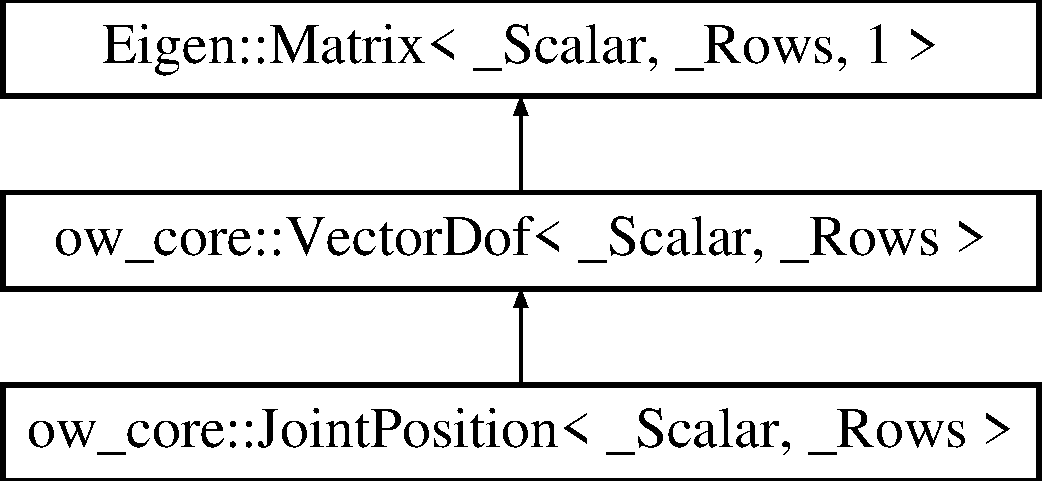
\includegraphics[height=3.000000cm]{da/d8e/classow__core_1_1JointPosition}
\end{center}
\end{figure}
\subsection*{Public Types}
\begin{DoxyCompactItemize}
\item 
enum \{ {\bfseries Rows} = \+\_\+\+Rows
 \}\hypertarget{classow__core_1_1JointPosition_a3bce0f7c54dfdda7d37141ac774d7a1c}{}\label{classow__core_1_1JointPosition_a3bce0f7c54dfdda7d37141ac774d7a1c}

\item 
typedef \+\_\+\+Scalar {\bfseries Scalar}\hypertarget{classow__core_1_1JointPosition_a1de340b233a2013396d800259b8fea54}{}\label{classow__core_1_1JointPosition_a1de340b233a2013396d800259b8fea54}

\item 
typedef \hyperlink{classow__core_1_1VectorDof}{Vector\+Dof}$<$ Scalar, Rows $>$ {\bfseries Base}\hypertarget{classow__core_1_1JointPosition_ad4e97b6ef198bc876f4ced4645de5403}{}\label{classow__core_1_1JointPosition_ad4e97b6ef198bc876f4ced4645de5403}

\end{DoxyCompactItemize}
\subsection*{Public Member Functions}
\begin{DoxyCompactItemize}
\item 
\hyperlink{classow__core_1_1JointPosition_a563520837683450f7ee71f7ba462868d}{Joint\+Position} ()\hypertarget{classow__core_1_1JointPosition_a563520837683450f7ee71f7ba462868d}{}\label{classow__core_1_1JointPosition_a563520837683450f7ee71f7ba462868d}

\begin{DoxyCompactList}\small\item\em Default Constructor. \end{DoxyCompactList}\item 
{\footnotesize template$<$typename Other\+Derived $>$ }\\\hyperlink{classow__core_1_1JointPosition_a10fe7d31f9b0af2fea545f72eb4c12b0}{Joint\+Position} (const Eigen\+::\+Eigen\+Base$<$ Other\+Derived $>$ \&other)
\begin{DoxyCompactList}\small\item\em Copy constructor. \end{DoxyCompactList}\end{DoxyCompactItemize}
\subsection*{Additional Inherited Members}


\subsection{Detailed Description}
\subsubsection*{template$<$typename \+\_\+\+Scalar, int \+\_\+\+Rows$>$\\*
class ow\+\_\+core\+::\+Joint\+Position$<$ \+\_\+\+Scalar, \+\_\+\+Rows $>$}

The \hyperlink{classow__core_1_1JointPosition}{Joint\+Position} class. 

The \hyperlink{classow__core_1_1JointPosition}{Joint\+Position} is of type \hyperlink{classow__core_1_1VectorDof}{Vector\+Dof} and is represented by the math symbol $\mathbf{q}$. 

\subsection{Constructor \& Destructor Documentation}
\index{ow\+\_\+core\+::\+Joint\+Position@{ow\+\_\+core\+::\+Joint\+Position}!Joint\+Position@{Joint\+Position}}
\index{Joint\+Position@{Joint\+Position}!ow\+\_\+core\+::\+Joint\+Position@{ow\+\_\+core\+::\+Joint\+Position}}
\subsubsection[{\texorpdfstring{Joint\+Position(const Eigen\+::\+Eigen\+Base$<$ Other\+Derived $>$ \&other)}{JointPosition(const Eigen::EigenBase< OtherDerived > &other)}}]{\setlength{\rightskip}{0pt plus 5cm}template$<$typename \+\_\+\+Scalar, int \+\_\+\+Rows$>$ template$<$typename Other\+Derived $>$ {\bf ow\+\_\+core\+::\+Joint\+Position}$<$ \+\_\+\+Scalar, \+\_\+\+Rows $>$\+::{\bf Joint\+Position} (
\begin{DoxyParamCaption}
\item[{const Eigen\+::\+Eigen\+Base$<$ Other\+Derived $>$ \&}]{other}
\end{DoxyParamCaption}
)\hspace{0.3cm}{\ttfamily [inline]}}\hypertarget{classow__core_1_1JointPosition_a10fe7d31f9b0af2fea545f72eb4c12b0}{}\label{classow__core_1_1JointPosition_a10fe7d31f9b0af2fea545f72eb4c12b0}


Copy constructor. 

This copy constructor not only works with Eigen matrices but also with their expressions. 

The documentation for this class was generated from the following file\+:\begin{DoxyCompactItemize}
\item 
/home/dean/ros/workspaces/ow\+\_\+test\+\_\+ws/src/ow\+\_\+core/include/ow\+\_\+core/\hyperlink{joint__position_8h}{joint\+\_\+position.\+h}\end{DoxyCompactItemize}

\hypertarget{classow__core_1_1JointState}{}\section{ow\+\_\+core\+:\+:Joint\+State$<$ \+\_\+\+Scalar, \+\_\+\+Rows $>$ Class Template Reference}
\label{classow__core_1_1JointState}\index{ow\+\_\+core\+::\+Joint\+State$<$ \+\_\+\+Scalar, \+\_\+\+Rows $>$@{ow\+\_\+core\+::\+Joint\+State$<$ \+\_\+\+Scalar, \+\_\+\+Rows $>$}}


The \hyperlink{classow__core_1_1JointState}{Joint\+State} class.  




{\ttfamily \#include $<$joint\+\_\+state.\+h$>$}

\subsection*{Public Types}
\begin{DoxyCompactItemize}
\item 
enum \{ {\bfseries Rows} = \+\_\+\+Rows
 \}\hypertarget{classow__core_1_1JointState_a72c9b5d1e8739f05cba3f4d877231f9f}{}\label{classow__core_1_1JointState_a72c9b5d1e8739f05cba3f4d877231f9f}

\item 
typedef \+\_\+\+Scalar {\bfseries Scalar}\hypertarget{classow__core_1_1JointState_aa4aedc0d11f33346be0481efeea485c9}{}\label{classow__core_1_1JointState_aa4aedc0d11f33346be0481efeea485c9}

\item 
typedef \hyperlink{classow__core_1_1VectorDof}{Vector\+Dof}$<$ Scalar, Rows $>$ {\bfseries J\+Vec}\hypertarget{classow__core_1_1JointState_a55aad096a0742060edcc4b13fda49215}{}\label{classow__core_1_1JointState_a55aad096a0742060edcc4b13fda49215}

\item 
typedef \hyperlink{classow__core_1_1JointPosition}{Joint\+Position}$<$ Scalar, Rows $>$ {\bfseries J\+Pos}\hypertarget{classow__core_1_1JointState_a9b3100d10fa3f1ae653453c4c661bb87}{}\label{classow__core_1_1JointState_a9b3100d10fa3f1ae653453c4c661bb87}

\item 
typedef \hyperlink{classow__core_1_1JointVelocity}{Joint\+Velocity}$<$ Scalar, Rows $>$ {\bfseries J\+Vel}\hypertarget{classow__core_1_1JointState_a9de74b73fb283026d2e7d505d1afc9fb}{}\label{classow__core_1_1JointState_a9de74b73fb283026d2e7d505d1afc9fb}

\item 
typedef \hyperlink{classow__core_1_1JointAcceleration}{Joint\+Acceleration}$<$ Scalar, Rows $>$ {\bfseries J\+Acc}\hypertarget{classow__core_1_1JointState_adecba7e0ecf7fd06d470f3dbde49127e}{}\label{classow__core_1_1JointState_adecba7e0ecf7fd06d470f3dbde49127e}

\item 
typedef \hyperlink{classow__core_1_1JointEffort}{Joint\+Effort}$<$ Scalar, Rows $>$ {\bfseries J\+Torque}\hypertarget{classow__core_1_1JointState_aee2a7252c178e5aae9742603bcca56f7}{}\label{classow__core_1_1JointState_aee2a7252c178e5aae9742603bcca56f7}

\end{DoxyCompactItemize}
\subsection*{Public Member Functions}
\begin{DoxyCompactItemize}
\item 
\hyperlink{classow__core_1_1JointState_a76834040169f792ff7a3c54d13fc34b7}{Joint\+State} ()\hypertarget{classow__core_1_1JointState_a76834040169f792ff7a3c54d13fc34b7}{}\label{classow__core_1_1JointState_a76834040169f792ff7a3c54d13fc34b7}

\begin{DoxyCompactList}\small\item\em Default Constructor. \end{DoxyCompactList}\item 
\hyperlink{classow__core_1_1JointPosition}{J\+Pos} \& {\bfseries q} ()\hypertarget{classow__core_1_1JointState_a185f41d427bc41b4136729c5f3fef0b8}{}\label{classow__core_1_1JointState_a185f41d427bc41b4136729c5f3fef0b8}

\item 
const \hyperlink{classow__core_1_1JointPosition}{J\+Pos} \& {\bfseries q} () const \hypertarget{classow__core_1_1JointState_ac270c084ab9f0fbafcc97e591faa896e}{}\label{classow__core_1_1JointState_ac270c084ab9f0fbafcc97e591faa896e}

\item 
\hyperlink{classow__core_1_1JointVelocity}{J\+Vel} \& {\bfseries qP} ()\hypertarget{classow__core_1_1JointState_a8cbbd546d0624376c328cf701d10d333}{}\label{classow__core_1_1JointState_a8cbbd546d0624376c328cf701d10d333}

\item 
const \hyperlink{classow__core_1_1JointVelocity}{J\+Vel} \& {\bfseries qP} () const \hypertarget{classow__core_1_1JointState_a57cc7ee7e3437d567f262e3c7747bdb1}{}\label{classow__core_1_1JointState_a57cc7ee7e3437d567f262e3c7747bdb1}

\item 
\hyperlink{classow__core_1_1JointAcceleration}{J\+Acc} \& {\bfseries q\+PP} ()\hypertarget{classow__core_1_1JointState_a6fc2f5adf0d20fb3682f25639b545125}{}\label{classow__core_1_1JointState_a6fc2f5adf0d20fb3682f25639b545125}

\item 
const \hyperlink{classow__core_1_1JointAcceleration}{J\+Acc} \& {\bfseries q\+PP} () const \hypertarget{classow__core_1_1JointState_a4acf99a2437e4dd9a654fd6cd4774ae7}{}\label{classow__core_1_1JointState_a4acf99a2437e4dd9a654fd6cd4774ae7}

\item 
\hyperlink{classow__core_1_1JointEffort}{J\+Torque} \& {\bfseries tau} ()\hypertarget{classow__core_1_1JointState_aa90b698b021686874d5243ca6d2e8da0}{}\label{classow__core_1_1JointState_aa90b698b021686874d5243ca6d2e8da0}

\item 
const \hyperlink{classow__core_1_1JointEffort}{J\+Torque} \& {\bfseries tau} () const \hypertarget{classow__core_1_1JointState_a09dd3ce70cbe13ce1abc59ecbffbfe15}{}\label{classow__core_1_1JointState_a09dd3ce70cbe13ce1abc59ecbffbfe15}

\end{DoxyCompactItemize}
\subsection*{Static Public Member Functions}
\begin{DoxyCompactItemize}
\item 
static const \hyperlink{classow__core_1_1JointState}{Joint\+State} \& {\bfseries Zero} ()\hypertarget{classow__core_1_1JointState_a2a27c25f103a202e19cbd00339931ef7}{}\label{classow__core_1_1JointState_a2a27c25f103a202e19cbd00339931ef7}

\end{DoxyCompactItemize}
\subsection*{Protected Attributes}
\begin{DoxyCompactItemize}
\item 
\hyperlink{classow__core_1_1JointPosition}{J\+Pos} {\bfseries q\+\_\+}\hypertarget{classow__core_1_1JointState_ae235da7bdc35c9fc7658fc17b0284a0d}{}\label{classow__core_1_1JointState_ae235da7bdc35c9fc7658fc17b0284a0d}

\item 
\hyperlink{classow__core_1_1JointVelocity}{J\+Vel} {\bfseries q\+P\+\_\+}\hypertarget{classow__core_1_1JointState_a1aba4e41fe47b16964cb356a499d235d}{}\label{classow__core_1_1JointState_a1aba4e41fe47b16964cb356a499d235d}

\item 
\hyperlink{classow__core_1_1JointAcceleration}{J\+Acc} {\bfseries q\+P\+P\+\_\+}\hypertarget{classow__core_1_1JointState_adc858e2b394646ed9ff139b162ca3967}{}\label{classow__core_1_1JointState_adc858e2b394646ed9ff139b162ca3967}

\item 
\hyperlink{classow__core_1_1JointEffort}{J\+Torque} {\bfseries tau\+\_\+}\hypertarget{classow__core_1_1JointState_a625cab6fc764fd1e2cba18e3b183fdd6}{}\label{classow__core_1_1JointState_a625cab6fc764fd1e2cba18e3b183fdd6}

\end{DoxyCompactItemize}


\subsection{Detailed Description}
\subsubsection*{template$<$typename \+\_\+\+Scalar, int \+\_\+\+Rows$>$\\*
class ow\+\_\+core\+::\+Joint\+State$<$ \+\_\+\+Scalar, \+\_\+\+Rows $>$}

The \hyperlink{classow__core_1_1JointState}{Joint\+State} class. 

This class is a container for\+:
\begin{DoxyItemize}
\item \hyperlink{classow__core_1_1JointPosition}{Joint\+Position}
\item \hyperlink{classow__core_1_1JointVelocity}{Joint\+Velocity}
\item \hyperlink{classow__core_1_1JointAcceleration}{Joint\+Acceleration}
\item \hyperlink{classow__core_1_1JointEffort}{Joint\+Effort} 
\end{DoxyItemize}

The documentation for this class was generated from the following file\+:\begin{DoxyCompactItemize}
\item 
/home/dean/ros/workspaces/ow\+\_\+test\+\_\+ws/src/ow\+\_\+core/include/ow\+\_\+core/\hyperlink{joint__state_8h}{joint\+\_\+state.\+h}\end{DoxyCompactItemize}

\hypertarget{classow__core_1_1JointVelocity}{}\section{ow\+\_\+core\+:\+:Joint\+Velocity$<$ \+\_\+\+Scalar, \+\_\+\+Rows $>$ Class Template Reference}
\label{classow__core_1_1JointVelocity}\index{ow\+\_\+core\+::\+Joint\+Velocity$<$ \+\_\+\+Scalar, \+\_\+\+Rows $>$@{ow\+\_\+core\+::\+Joint\+Velocity$<$ \+\_\+\+Scalar, \+\_\+\+Rows $>$}}


The \hyperlink{classow__core_1_1JointVelocity}{Joint\+Velocity} class.  




{\ttfamily \#include $<$joint\+\_\+velocity.\+h$>$}

Inheritance diagram for ow\+\_\+core\+:\+:Joint\+Velocity$<$ \+\_\+\+Scalar, \+\_\+\+Rows $>$\+:\begin{figure}[H]
\begin{center}
\leavevmode
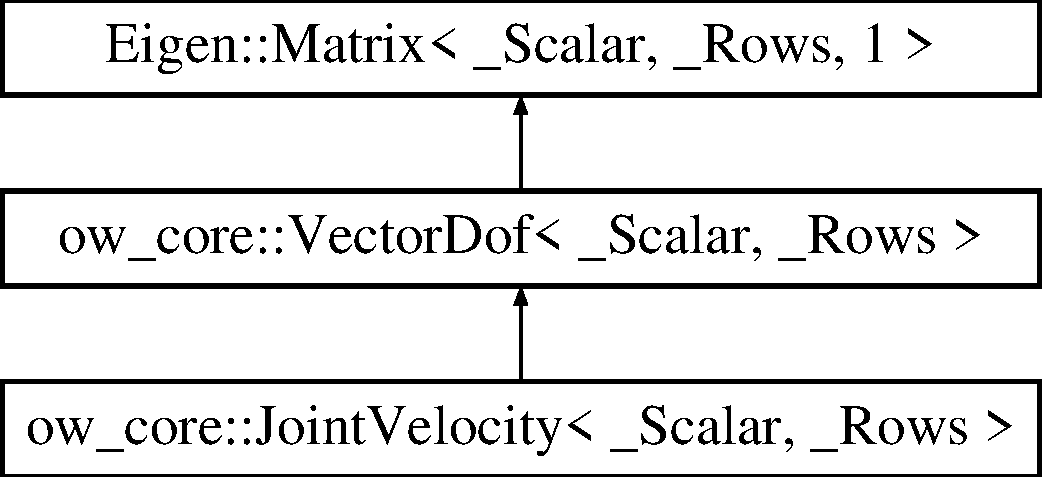
\includegraphics[height=3.000000cm]{da/d5f/classow__core_1_1JointVelocity}
\end{center}
\end{figure}
\subsection*{Public Types}
\begin{DoxyCompactItemize}
\item 
enum \{ {\bfseries Rows} = \+\_\+\+Rows
 \}\hypertarget{classow__core_1_1JointVelocity_a75add96357b65cd35fa5edf5275439b7}{}\label{classow__core_1_1JointVelocity_a75add96357b65cd35fa5edf5275439b7}

\item 
typedef \+\_\+\+Scalar {\bfseries Scalar}\hypertarget{classow__core_1_1JointVelocity_a4e972bf4b9e3204bd9074f3f22f9bef2}{}\label{classow__core_1_1JointVelocity_a4e972bf4b9e3204bd9074f3f22f9bef2}

\item 
typedef \hyperlink{classow__core_1_1VectorDof}{Vector\+Dof}$<$ Scalar, Rows $>$ {\bfseries Base}\hypertarget{classow__core_1_1JointVelocity_a85aa20acbd125d605c5e54dc7505e3cd}{}\label{classow__core_1_1JointVelocity_a85aa20acbd125d605c5e54dc7505e3cd}

\end{DoxyCompactItemize}
\subsection*{Public Member Functions}
\begin{DoxyCompactItemize}
\item 
\hyperlink{classow__core_1_1JointVelocity_a4441b48524439cbd670908be707c3ed8}{Joint\+Velocity} ()\hypertarget{classow__core_1_1JointVelocity_a4441b48524439cbd670908be707c3ed8}{}\label{classow__core_1_1JointVelocity_a4441b48524439cbd670908be707c3ed8}

\begin{DoxyCompactList}\small\item\em Default Constructor. \end{DoxyCompactList}\item 
{\footnotesize template$<$typename Other\+Derived $>$ }\\\hyperlink{classow__core_1_1JointVelocity_ae94c411048769beee3a1623a4cb3ee91}{Joint\+Velocity} (const Eigen\+::\+Eigen\+Base$<$ Other\+Derived $>$ \&other)
\begin{DoxyCompactList}\small\item\em Copy constructor. \end{DoxyCompactList}\end{DoxyCompactItemize}
\subsection*{Additional Inherited Members}


\subsection{Detailed Description}
\subsubsection*{template$<$typename \+\_\+\+Scalar, int \+\_\+\+Rows$>$\\*
class ow\+\_\+core\+::\+Joint\+Velocity$<$ \+\_\+\+Scalar, \+\_\+\+Rows $>$}

The \hyperlink{classow__core_1_1JointVelocity}{Joint\+Velocity} class. 

The \hyperlink{classow__core_1_1JointVelocity}{Joint\+Velocity} is of type \hyperlink{classow__core_1_1VectorDof}{Vector\+Dof} and is represented by the math symbol $\mathbf{\dot{q}}$. 

\subsection{Constructor \& Destructor Documentation}
\index{ow\+\_\+core\+::\+Joint\+Velocity@{ow\+\_\+core\+::\+Joint\+Velocity}!Joint\+Velocity@{Joint\+Velocity}}
\index{Joint\+Velocity@{Joint\+Velocity}!ow\+\_\+core\+::\+Joint\+Velocity@{ow\+\_\+core\+::\+Joint\+Velocity}}
\subsubsection[{\texorpdfstring{Joint\+Velocity(const Eigen\+::\+Eigen\+Base$<$ Other\+Derived $>$ \&other)}{JointVelocity(const Eigen::EigenBase< OtherDerived > &other)}}]{\setlength{\rightskip}{0pt plus 5cm}template$<$typename \+\_\+\+Scalar, int \+\_\+\+Rows$>$ template$<$typename Other\+Derived $>$ {\bf ow\+\_\+core\+::\+Joint\+Velocity}$<$ \+\_\+\+Scalar, \+\_\+\+Rows $>$\+::{\bf Joint\+Velocity} (
\begin{DoxyParamCaption}
\item[{const Eigen\+::\+Eigen\+Base$<$ Other\+Derived $>$ \&}]{other}
\end{DoxyParamCaption}
)\hspace{0.3cm}{\ttfamily [inline]}}\hypertarget{classow__core_1_1JointVelocity_ae94c411048769beee3a1623a4cb3ee91}{}\label{classow__core_1_1JointVelocity_ae94c411048769beee3a1623a4cb3ee91}


Copy constructor. 

This copy constructor not only works with Eigen matrices but also with their expressions. 

The documentation for this class was generated from the following file\+:\begin{DoxyCompactItemize}
\item 
/home/dean/ros/workspaces/ow\+\_\+test\+\_\+ws/src/ow\+\_\+core/include/ow\+\_\+core/\hyperlink{joint__velocity_8h}{joint\+\_\+velocity.\+h}\end{DoxyCompactItemize}

\hypertarget{classow__core_1_1LinearAcceleration}{}\section{ow\+\_\+core\+:\+:Linear\+Acceleration$<$ \+\_\+\+Scalar $>$ Class Template Reference}
\label{classow__core_1_1LinearAcceleration}\index{ow\+\_\+core\+::\+Linear\+Acceleration$<$ \+\_\+\+Scalar $>$@{ow\+\_\+core\+::\+Linear\+Acceleration$<$ \+\_\+\+Scalar $>$}}


The \hyperlink{classow__core_1_1LinearAcceleration}{Linear\+Acceleration} class.  




{\ttfamily \#include $<$linear\+\_\+acceleration.\+h$>$}

Inheritance diagram for ow\+\_\+core\+:\+:Linear\+Acceleration$<$ \+\_\+\+Scalar $>$\+:\begin{figure}[H]
\begin{center}
\leavevmode
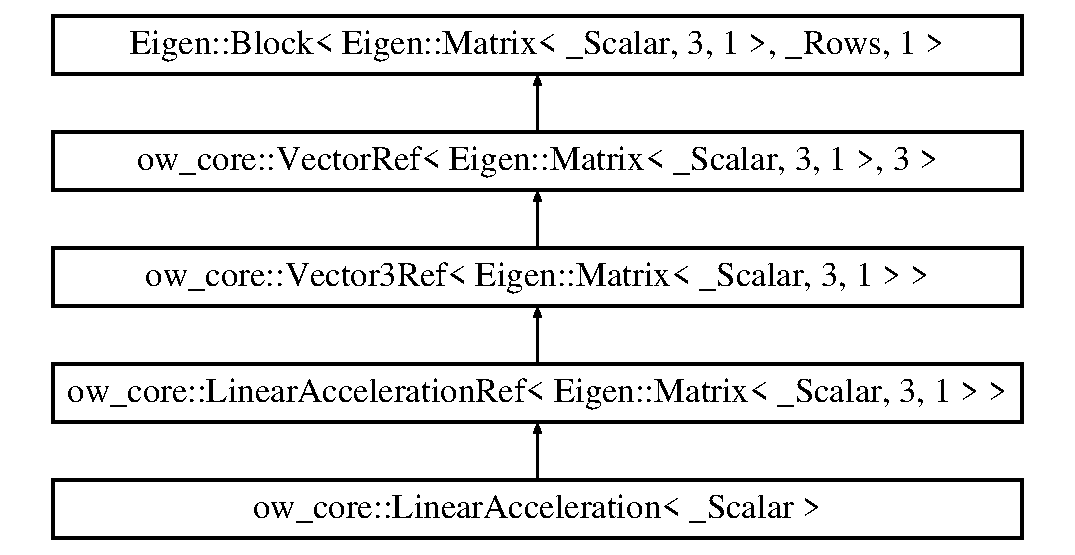
\includegraphics[height=5.000000cm]{d2/d41/classow__core_1_1LinearAcceleration}
\end{center}
\end{figure}
\subsection*{Public Types}
\begin{DoxyCompactItemize}
\item 
typedef \+\_\+\+Scalar {\bfseries Scalar}\hypertarget{classow__core_1_1LinearAcceleration_a11f5e96fae3ce2a9833d73dc64a9854c}{}\label{classow__core_1_1LinearAcceleration_a11f5e96fae3ce2a9833d73dc64a9854c}

\item 
typedef Eigen\+::\+Matrix$<$ \+\_\+\+Scalar, 3, 1 $>$ {\bfseries Derived}\hypertarget{classow__core_1_1LinearAcceleration_a964ade2d7efcfa7dd3876e779ccd13c5}{}\label{classow__core_1_1LinearAcceleration_a964ade2d7efcfa7dd3876e779ccd13c5}

\item 
typedef \hyperlink{classow__core_1_1LinearAccelerationRef}{Linear\+Acceleration\+Ref}$<$ Derived $>$ {\bfseries Base}\hypertarget{classow__core_1_1LinearAcceleration_ae577feb121ea5253b6d68b08f2d8af44}{}\label{classow__core_1_1LinearAcceleration_ae577feb121ea5253b6d68b08f2d8af44}

\end{DoxyCompactItemize}
\subsection*{Public Member Functions}
\begin{DoxyCompactItemize}
\item 
\hyperlink{classow__core_1_1LinearAcceleration_a6761e3ab1a7bd77c15cb0759dd25b1e1}{Linear\+Acceleration} ()\hypertarget{classow__core_1_1LinearAcceleration_a6761e3ab1a7bd77c15cb0759dd25b1e1}{}\label{classow__core_1_1LinearAcceleration_a6761e3ab1a7bd77c15cb0759dd25b1e1}

\begin{DoxyCompactList}\small\item\em Default Constructor. \end{DoxyCompactList}\item 
\hyperlink{classow__core_1_1LinearAcceleration_ae2ac66af1c81554f31535fd7af7aa2b4}{Linear\+Acceleration} (const Scalar \&x, const Scalar \&y, const Scalar \&z)\hypertarget{classow__core_1_1LinearAcceleration_ae2ac66af1c81554f31535fd7af7aa2b4}{}\label{classow__core_1_1LinearAcceleration_ae2ac66af1c81554f31535fd7af7aa2b4}

\begin{DoxyCompactList}\small\item\em Assignment from Scalar values. \end{DoxyCompactList}\item 
{\footnotesize template$<$typename Other\+Derived $>$ }\\\hyperlink{classow__core_1_1LinearAcceleration_a243335c29a665db0eb2870fa7d41f5eb}{Linear\+Acceleration} (const Eigen\+::\+Eigen\+Base$<$ Other\+Derived $>$ \&other)
\begin{DoxyCompactList}\small\item\em Copy constructor. \end{DoxyCompactList}\end{DoxyCompactItemize}
\subsection*{Protected Attributes}
\begin{DoxyCompactItemize}
\item 
Derived {\bfseries data\+\_\+}\hypertarget{classow__core_1_1LinearAcceleration_aaf5e7a060e1ed0ac2f3545ba4485fe36}{}\label{classow__core_1_1LinearAcceleration_aaf5e7a060e1ed0ac2f3545ba4485fe36}

\end{DoxyCompactItemize}


\subsection{Detailed Description}
\subsubsection*{template$<$typename \+\_\+\+Scalar$>$\\*
class ow\+\_\+core\+::\+Linear\+Acceleration$<$ \+\_\+\+Scalar $>$}

The \hyperlink{classow__core_1_1LinearAcceleration}{Linear\+Acceleration} class. 

The \hyperlink{classow__core_1_1LinearAcceleration}{Linear\+Acceleration} is of type Eigen\+::\+Vector3 and is represented by the math symbol $\ddot{\mathbf{x}}$. 

\subsection{Constructor \& Destructor Documentation}
\index{ow\+\_\+core\+::\+Linear\+Acceleration@{ow\+\_\+core\+::\+Linear\+Acceleration}!Linear\+Acceleration@{Linear\+Acceleration}}
\index{Linear\+Acceleration@{Linear\+Acceleration}!ow\+\_\+core\+::\+Linear\+Acceleration@{ow\+\_\+core\+::\+Linear\+Acceleration}}
\subsubsection[{\texorpdfstring{Linear\+Acceleration(const Eigen\+::\+Eigen\+Base$<$ Other\+Derived $>$ \&other)}{LinearAcceleration(const Eigen::EigenBase< OtherDerived > &other)}}]{\setlength{\rightskip}{0pt plus 5cm}template$<$typename \+\_\+\+Scalar$>$ template$<$typename Other\+Derived $>$ {\bf ow\+\_\+core\+::\+Linear\+Acceleration}$<$ \+\_\+\+Scalar $>$\+::{\bf Linear\+Acceleration} (
\begin{DoxyParamCaption}
\item[{const Eigen\+::\+Eigen\+Base$<$ Other\+Derived $>$ \&}]{other}
\end{DoxyParamCaption}
)\hspace{0.3cm}{\ttfamily [inline]}}\hypertarget{classow__core_1_1LinearAcceleration_a243335c29a665db0eb2870fa7d41f5eb}{}\label{classow__core_1_1LinearAcceleration_a243335c29a665db0eb2870fa7d41f5eb}


Copy constructor. 

This copy constructor not only works with Eigen matrices but also with their expressions. 

The documentation for this class was generated from the following file\+:\begin{DoxyCompactItemize}
\item 
/home/dean/ros/workspaces/ow\+\_\+test\+\_\+ws/src/ow\+\_\+core/include/ow\+\_\+core/\hyperlink{linear__acceleration_8h}{linear\+\_\+acceleration.\+h}\end{DoxyCompactItemize}

\hypertarget{classow__core_1_1LinearAccelerationRef}{}\section{ow\+\_\+core\+:\+:Linear\+Acceleration\+Ref$<$ \+\_\+\+Derived $>$ Class Template Reference}
\label{classow__core_1_1LinearAccelerationRef}\index{ow\+\_\+core\+::\+Linear\+Acceleration\+Ref$<$ \+\_\+\+Derived $>$@{ow\+\_\+core\+::\+Linear\+Acceleration\+Ref$<$ \+\_\+\+Derived $>$}}


The \hyperlink{classow__core_1_1LinearAccelerationRef}{Linear\+Acceleration\+Ref} class.  




{\ttfamily \#include $<$linear\+\_\+acceleration\+\_\+ref.\+h$>$}

Inheritance diagram for ow\+\_\+core\+:\+:Linear\+Acceleration\+Ref$<$ \+\_\+\+Derived $>$\+:\begin{figure}[H]
\begin{center}
\leavevmode
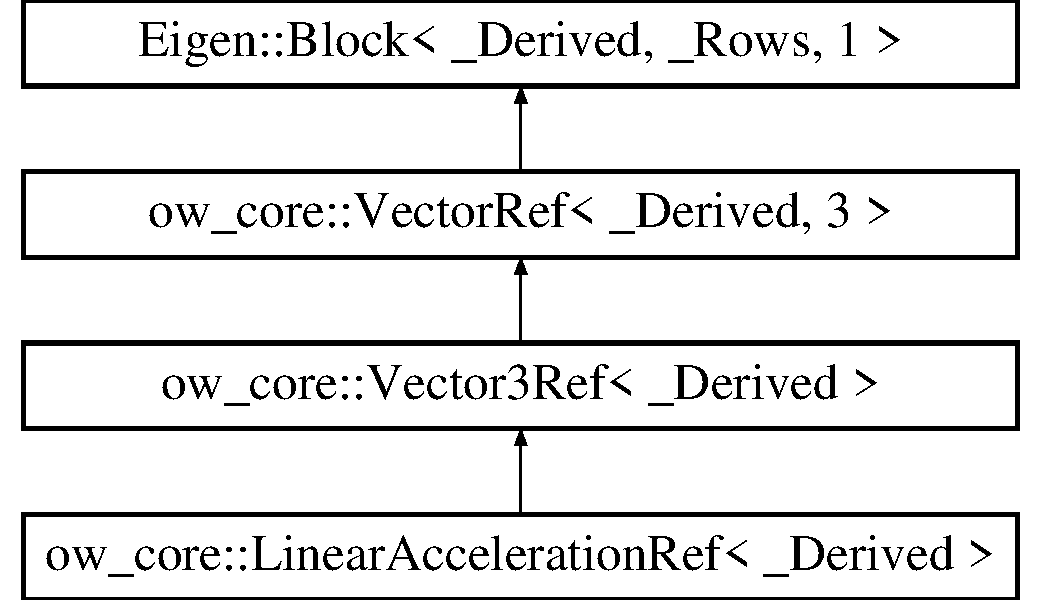
\includegraphics[height=4.000000cm]{d2/d75/classow__core_1_1LinearAccelerationRef}
\end{center}
\end{figure}
\subsection*{Public Types}
\begin{DoxyCompactItemize}
\item 
typedef \+\_\+\+Derived {\bfseries Derived}\hypertarget{classow__core_1_1LinearAccelerationRef_aba03ae2dd6572abc254c71c0b4032bd1}{}\label{classow__core_1_1LinearAccelerationRef_aba03ae2dd6572abc254c71c0b4032bd1}

\item 
typedef \hyperlink{classow__core_1_1Vector3Ref}{Vector3\+Ref}$<$ Derived $>$ {\bfseries Base}\hypertarget{classow__core_1_1LinearAccelerationRef_ae563452edb03b1441c6388427df13ad0}{}\label{classow__core_1_1LinearAccelerationRef_ae563452edb03b1441c6388427df13ad0}

\end{DoxyCompactItemize}
\subsection*{Public Member Functions}
\begin{DoxyCompactItemize}
\item 
\hyperlink{classow__core_1_1LinearAccelerationRef_a16b61c66d54fcc5e59eef31489dc2c4a}{Linear\+Acceleration\+Ref} (Derived \&ref, int start\+Row=0, int start\+Col=0)
\begin{DoxyCompactList}\small\item\em Default Constructor. \end{DoxyCompactList}\end{DoxyCompactItemize}


\subsection{Detailed Description}
\subsubsection*{template$<$typename \+\_\+\+Derived$>$\\*
class ow\+\_\+core\+::\+Linear\+Acceleration\+Ref$<$ \+\_\+\+Derived $>$}

The \hyperlink{classow__core_1_1LinearAccelerationRef}{Linear\+Acceleration\+Ref} class. 

The \hyperlink{classow__core_1_1LinearAcceleration}{Linear\+Acceleration} is of type Eigen\+::\+Vector3 and is represented by the math symbol $\ddot{\mathbf{x}}$.

References the data of another Eigen type class via Eigen\+::\+Block. 

\subsection{Constructor \& Destructor Documentation}
\index{ow\+\_\+core\+::\+Linear\+Acceleration\+Ref@{ow\+\_\+core\+::\+Linear\+Acceleration\+Ref}!Linear\+Acceleration\+Ref@{Linear\+Acceleration\+Ref}}
\index{Linear\+Acceleration\+Ref@{Linear\+Acceleration\+Ref}!ow\+\_\+core\+::\+Linear\+Acceleration\+Ref@{ow\+\_\+core\+::\+Linear\+Acceleration\+Ref}}
\subsubsection[{\texorpdfstring{Linear\+Acceleration\+Ref(\+Derived \&ref, int start\+Row=0, int start\+Col=0)}{LinearAccelerationRef(Derived &ref, int startRow=0, int startCol=0)}}]{\setlength{\rightskip}{0pt plus 5cm}template$<$typename \+\_\+\+Derived$>$ {\bf ow\+\_\+core\+::\+Linear\+Acceleration\+Ref}$<$ \+\_\+\+Derived $>$\+::{\bf Linear\+Acceleration\+Ref} (
\begin{DoxyParamCaption}
\item[{Derived \&}]{ref, }
\item[{int}]{start\+Row = {\ttfamily 0}, }
\item[{int}]{start\+Col = {\ttfamily 0}}
\end{DoxyParamCaption}
)\hspace{0.3cm}{\ttfamily [inline]}, {\ttfamily [explicit]}}\hypertarget{classow__core_1_1LinearAccelerationRef_a16b61c66d54fcc5e59eef31489dc2c4a}{}\label{classow__core_1_1LinearAccelerationRef_a16b61c66d54fcc5e59eef31489dc2c4a}


Default Constructor. 


\begin{DoxyParams}{Parameters}
{\em ref} & the reference to storage Eigen object to access the elements of the \hyperlink{classow__core_1_1LinearAcceleration}{Linear\+Acceleration} via Eigen\+::\+Block.\\
\hline
{\em start\+Row} & the start index of the row for Eigen\+::\+Block.\\
\hline
{\em start\+Col} & the start index of the column for Eigen\+::\+Block. \\
\hline
\end{DoxyParams}


The documentation for this class was generated from the following file\+:\begin{DoxyCompactItemize}
\item 
/home/dean/ros/workspaces/ow\+\_\+test\+\_\+ws/src/ow\+\_\+core/include/ow\+\_\+core/\hyperlink{linear__acceleration__ref_8h}{linear\+\_\+acceleration\+\_\+ref.\+h}\end{DoxyCompactItemize}

\hypertarget{classow__core_1_1LinearPosition}{}\section{ow\+\_\+core\+:\+:Linear\+Position$<$ \+\_\+\+Scalar $>$ Class Template Reference}
\label{classow__core_1_1LinearPosition}\index{ow\+\_\+core\+::\+Linear\+Position$<$ \+\_\+\+Scalar $>$@{ow\+\_\+core\+::\+Linear\+Position$<$ \+\_\+\+Scalar $>$}}


The \hyperlink{classow__core_1_1LinearPosition}{Linear\+Position} class.  




{\ttfamily \#include $<$linear\+\_\+position.\+h$>$}

Inheritance diagram for ow\+\_\+core\+:\+:Linear\+Position$<$ \+\_\+\+Scalar $>$\+:\begin{figure}[H]
\begin{center}
\leavevmode
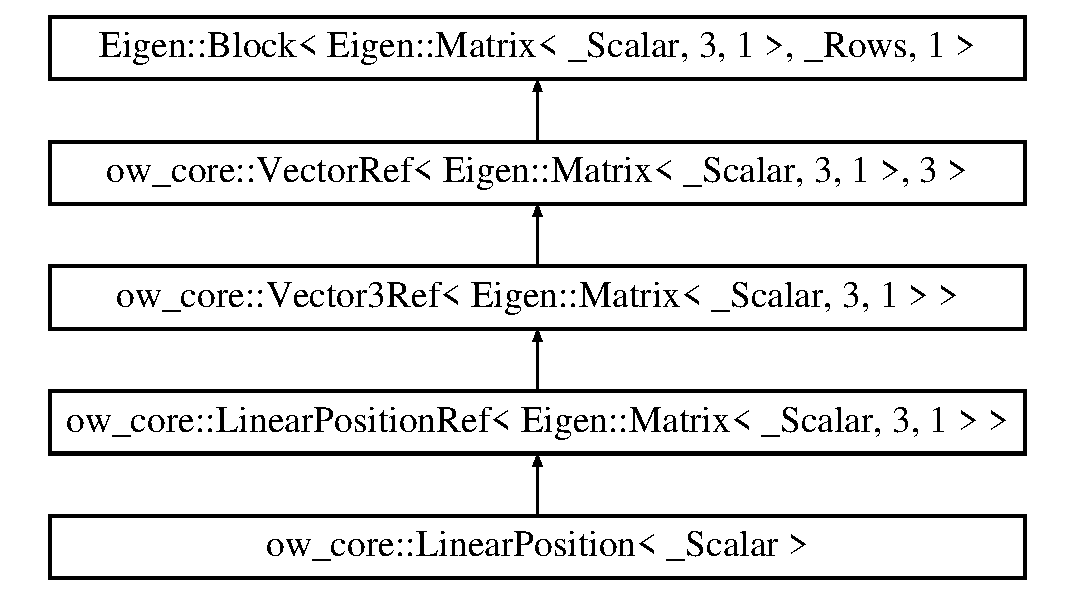
\includegraphics[height=5.000000cm]{d1/db1/classow__core_1_1LinearPosition}
\end{center}
\end{figure}
\subsection*{Public Types}
\begin{DoxyCompactItemize}
\item 
typedef \+\_\+\+Scalar {\bfseries Scalar}\hypertarget{classow__core_1_1LinearPosition_a0102d94ddb84aaf861ce5bcbadcec713}{}\label{classow__core_1_1LinearPosition_a0102d94ddb84aaf861ce5bcbadcec713}

\item 
typedef Eigen\+::\+Matrix$<$ \+\_\+\+Scalar, 3, 1 $>$ {\bfseries Derived}\hypertarget{classow__core_1_1LinearPosition_aa9f7c4a728c84a23a45904622ec6ece7}{}\label{classow__core_1_1LinearPosition_aa9f7c4a728c84a23a45904622ec6ece7}

\item 
typedef \hyperlink{classow__core_1_1LinearPositionRef}{Linear\+Position\+Ref}$<$ Derived $>$ {\bfseries Base}\hypertarget{classow__core_1_1LinearPosition_ab6605ce95de0423dcf22ad80806eb6d0}{}\label{classow__core_1_1LinearPosition_ab6605ce95de0423dcf22ad80806eb6d0}

\end{DoxyCompactItemize}
\subsection*{Public Member Functions}
\begin{DoxyCompactItemize}
\item 
\hyperlink{classow__core_1_1LinearPosition_a2ef1d8e782a06e13acd52130f3e2f503}{Linear\+Position} ()\hypertarget{classow__core_1_1LinearPosition_a2ef1d8e782a06e13acd52130f3e2f503}{}\label{classow__core_1_1LinearPosition_a2ef1d8e782a06e13acd52130f3e2f503}

\begin{DoxyCompactList}\small\item\em Default Constructor. \end{DoxyCompactList}\item 
\hyperlink{classow__core_1_1LinearPosition_af540e92398f5d2e28456118570cc3a8e}{Linear\+Position} (const Scalar \&x, const Scalar \&y, const Scalar \&z)\hypertarget{classow__core_1_1LinearPosition_af540e92398f5d2e28456118570cc3a8e}{}\label{classow__core_1_1LinearPosition_af540e92398f5d2e28456118570cc3a8e}

\begin{DoxyCompactList}\small\item\em Assignment from Scalar values. \end{DoxyCompactList}\item 
{\footnotesize template$<$typename Other\+Derived $>$ }\\\hyperlink{classow__core_1_1LinearPosition_aaee24489f4658cb2302f28db12c5f678}{Linear\+Position} (const Eigen\+::\+Eigen\+Base$<$ Other\+Derived $>$ \&other)
\begin{DoxyCompactList}\small\item\em Copy constructor. \end{DoxyCompactList}\end{DoxyCompactItemize}
\subsection*{Protected Attributes}
\begin{DoxyCompactItemize}
\item 
Derived {\bfseries data\+\_\+}\hypertarget{classow__core_1_1LinearPosition_a99b2abe7e251b1f1be6a6a5343541ecf}{}\label{classow__core_1_1LinearPosition_a99b2abe7e251b1f1be6a6a5343541ecf}

\end{DoxyCompactItemize}


\subsection{Detailed Description}
\subsubsection*{template$<$typename \+\_\+\+Scalar$>$\\*
class ow\+\_\+core\+::\+Linear\+Position$<$ \+\_\+\+Scalar $>$}

The \hyperlink{classow__core_1_1LinearPosition}{Linear\+Position} class. 

The \hyperlink{classow__core_1_1LinearPosition}{Linear\+Position} is of type Eigen\+::\+Vector3 and is represented by the math symbol $\mathbf{x}$. 

\subsection{Constructor \& Destructor Documentation}
\index{ow\+\_\+core\+::\+Linear\+Position@{ow\+\_\+core\+::\+Linear\+Position}!Linear\+Position@{Linear\+Position}}
\index{Linear\+Position@{Linear\+Position}!ow\+\_\+core\+::\+Linear\+Position@{ow\+\_\+core\+::\+Linear\+Position}}
\subsubsection[{\texorpdfstring{Linear\+Position(const Eigen\+::\+Eigen\+Base$<$ Other\+Derived $>$ \&other)}{LinearPosition(const Eigen::EigenBase< OtherDerived > &other)}}]{\setlength{\rightskip}{0pt plus 5cm}template$<$typename \+\_\+\+Scalar $>$ template$<$typename Other\+Derived $>$ {\bf ow\+\_\+core\+::\+Linear\+Position}$<$ \+\_\+\+Scalar $>$\+::{\bf Linear\+Position} (
\begin{DoxyParamCaption}
\item[{const Eigen\+::\+Eigen\+Base$<$ Other\+Derived $>$ \&}]{other}
\end{DoxyParamCaption}
)\hspace{0.3cm}{\ttfamily [inline]}}\hypertarget{classow__core_1_1LinearPosition_aaee24489f4658cb2302f28db12c5f678}{}\label{classow__core_1_1LinearPosition_aaee24489f4658cb2302f28db12c5f678}


Copy constructor. 

This copy constructor not only works with Eigen matrices but also with their expressions. 

The documentation for this class was generated from the following file\+:\begin{DoxyCompactItemize}
\item 
/home/dean/ros/workspaces/ow\+\_\+test\+\_\+ws/src/ow\+\_\+core/include/ow\+\_\+core/\hyperlink{linear__position_8h}{linear\+\_\+position.\+h}\end{DoxyCompactItemize}

\hypertarget{classow__core_1_1LinearPositionRef}{}\section{ow\+\_\+core\+:\+:Linear\+Position\+Ref$<$ \+\_\+\+Derived $>$ Class Template Reference}
\label{classow__core_1_1LinearPositionRef}\index{ow\+\_\+core\+::\+Linear\+Position\+Ref$<$ \+\_\+\+Derived $>$@{ow\+\_\+core\+::\+Linear\+Position\+Ref$<$ \+\_\+\+Derived $>$}}


The \hyperlink{classow__core_1_1LinearPositionRef}{Linear\+Position\+Ref} class.  




{\ttfamily \#include $<$linear\+\_\+position\+\_\+ref.\+h$>$}

Inheritance diagram for ow\+\_\+core\+:\+:Linear\+Position\+Ref$<$ \+\_\+\+Derived $>$\+:\begin{figure}[H]
\begin{center}
\leavevmode
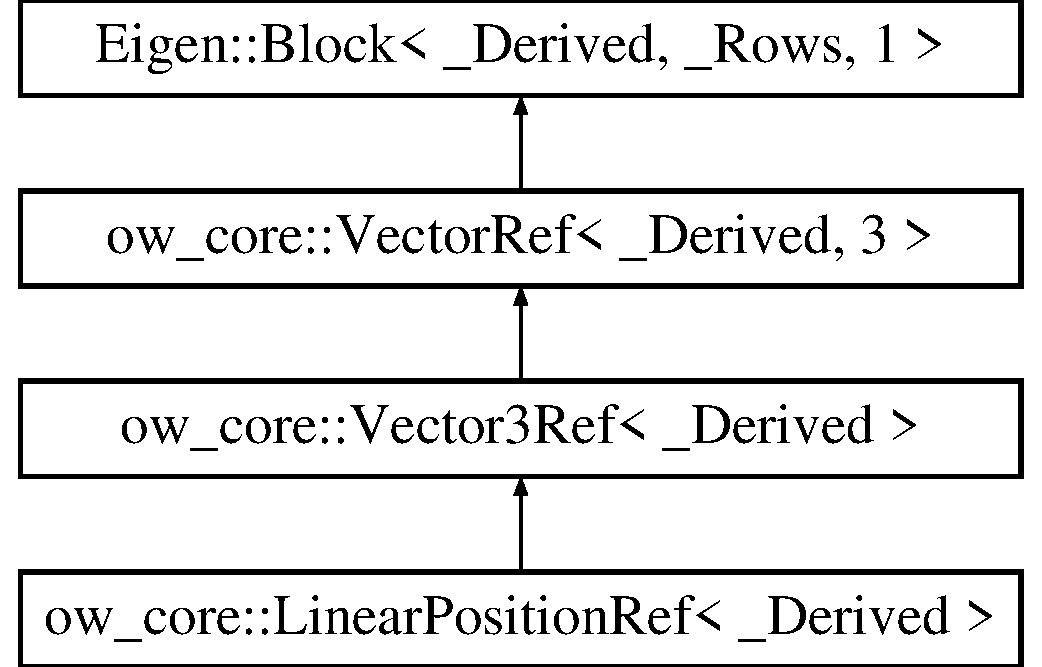
\includegraphics[height=4.000000cm]{da/d4c/classow__core_1_1LinearPositionRef}
\end{center}
\end{figure}
\subsection*{Public Types}
\begin{DoxyCompactItemize}
\item 
typedef \+\_\+\+Derived {\bfseries Derived}\hypertarget{classow__core_1_1LinearPositionRef_a44d84d26f5ce03cb78cb010c148e9553}{}\label{classow__core_1_1LinearPositionRef_a44d84d26f5ce03cb78cb010c148e9553}

\item 
typedef \hyperlink{classow__core_1_1Vector3Ref}{Vector3\+Ref}$<$ Derived $>$ {\bfseries Base}\hypertarget{classow__core_1_1LinearPositionRef_aa1bd5a9697af32ea64d5ef320b93362f}{}\label{classow__core_1_1LinearPositionRef_aa1bd5a9697af32ea64d5ef320b93362f}

\end{DoxyCompactItemize}
\subsection*{Public Member Functions}
\begin{DoxyCompactItemize}
\item 
\hyperlink{classow__core_1_1LinearPositionRef_a5e8d28ff1c2e36eaefe533017d27c8aa}{Linear\+Position\+Ref} (Derived \&ref, int start\+Row=0, int start\+Col=0)
\begin{DoxyCompactList}\small\item\em Default Constructor. \end{DoxyCompactList}\end{DoxyCompactItemize}


\subsection{Detailed Description}
\subsubsection*{template$<$typename \+\_\+\+Derived$>$\\*
class ow\+\_\+core\+::\+Linear\+Position\+Ref$<$ \+\_\+\+Derived $>$}

The \hyperlink{classow__core_1_1LinearPositionRef}{Linear\+Position\+Ref} class. 

The \hyperlink{classow__core_1_1LinearPositionRef}{Linear\+Position\+Ref} is of type Eigen\+::\+Vector3 and is represented by the math symbol $\mathbf{x}$.

References the data of another Eigen type class via Eigen\+::\+Block. 

\subsection{Constructor \& Destructor Documentation}
\index{ow\+\_\+core\+::\+Linear\+Position\+Ref@{ow\+\_\+core\+::\+Linear\+Position\+Ref}!Linear\+Position\+Ref@{Linear\+Position\+Ref}}
\index{Linear\+Position\+Ref@{Linear\+Position\+Ref}!ow\+\_\+core\+::\+Linear\+Position\+Ref@{ow\+\_\+core\+::\+Linear\+Position\+Ref}}
\subsubsection[{\texorpdfstring{Linear\+Position\+Ref(\+Derived \&ref, int start\+Row=0, int start\+Col=0)}{LinearPositionRef(Derived &ref, int startRow=0, int startCol=0)}}]{\setlength{\rightskip}{0pt plus 5cm}template$<$typename \+\_\+\+Derived$>$ {\bf ow\+\_\+core\+::\+Linear\+Position\+Ref}$<$ \+\_\+\+Derived $>$\+::{\bf Linear\+Position\+Ref} (
\begin{DoxyParamCaption}
\item[{Derived \&}]{ref, }
\item[{int}]{start\+Row = {\ttfamily 0}, }
\item[{int}]{start\+Col = {\ttfamily 0}}
\end{DoxyParamCaption}
)\hspace{0.3cm}{\ttfamily [inline]}, {\ttfamily [explicit]}}\hypertarget{classow__core_1_1LinearPositionRef_a5e8d28ff1c2e36eaefe533017d27c8aa}{}\label{classow__core_1_1LinearPositionRef_a5e8d28ff1c2e36eaefe533017d27c8aa}


Default Constructor. 


\begin{DoxyParams}{Parameters}
{\em ref} & the reference to storage Eigen object to access the elements of the \hyperlink{classow__core_1_1LinearPosition}{Linear\+Position} via Eigen\+::\+Block.\\
\hline
{\em start\+Row} & the start index of the row for Eigen\+::\+Block.\\
\hline
{\em start\+Col} & the start index of the column for Eigen\+::\+Block. \\
\hline
\end{DoxyParams}


The documentation for this class was generated from the following file\+:\begin{DoxyCompactItemize}
\item 
/home/dean/ros/workspaces/ow\+\_\+test\+\_\+ws/src/ow\+\_\+core/include/ow\+\_\+core/\hyperlink{linear__position__ref_8h}{linear\+\_\+position\+\_\+ref.\+h}\end{DoxyCompactItemize}

\hypertarget{classow__core_1_1LinearVelocity}{}\section{ow\+\_\+core\+:\+:Linear\+Velocity$<$ \+\_\+\+Scalar $>$ Class Template Reference}
\label{classow__core_1_1LinearVelocity}\index{ow\+\_\+core\+::\+Linear\+Velocity$<$ \+\_\+\+Scalar $>$@{ow\+\_\+core\+::\+Linear\+Velocity$<$ \+\_\+\+Scalar $>$}}


The \hyperlink{classow__core_1_1LinearVelocity}{Linear\+Velocity} class.  




{\ttfamily \#include $<$linear\+\_\+velocity.\+h$>$}

Inheritance diagram for ow\+\_\+core\+:\+:Linear\+Velocity$<$ \+\_\+\+Scalar $>$\+:\begin{figure}[H]
\begin{center}
\leavevmode
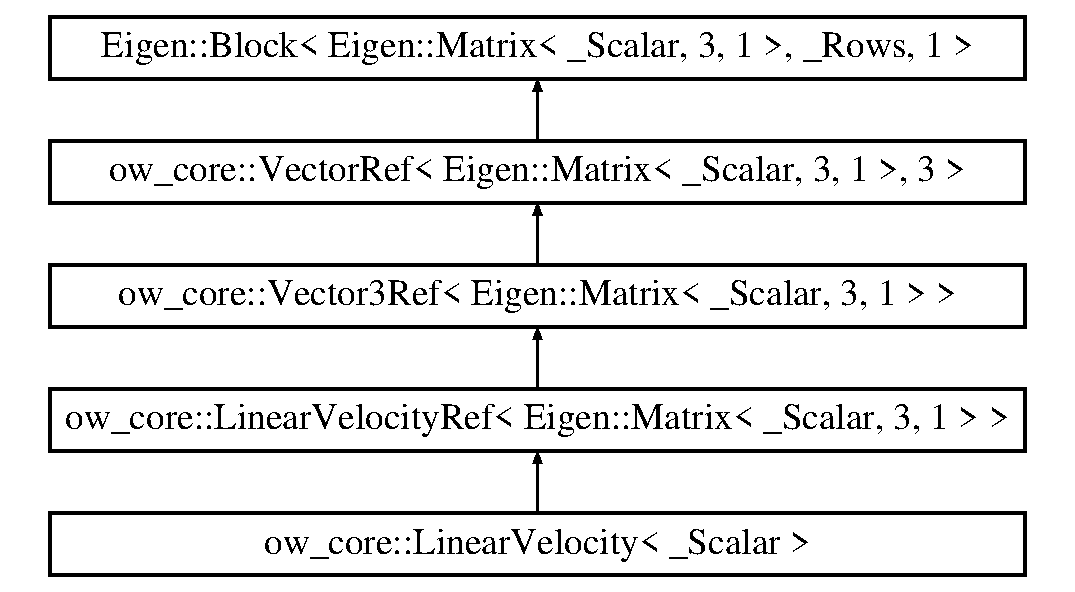
\includegraphics[height=5.000000cm]{d3/d6e/classow__core_1_1LinearVelocity}
\end{center}
\end{figure}
\subsection*{Public Types}
\begin{DoxyCompactItemize}
\item 
typedef \+\_\+\+Scalar {\bfseries Scalar}\hypertarget{classow__core_1_1LinearVelocity_a088145bea5e0ce67c36e3704f2d302b1}{}\label{classow__core_1_1LinearVelocity_a088145bea5e0ce67c36e3704f2d302b1}

\item 
typedef Eigen\+::\+Matrix$<$ \+\_\+\+Scalar, 3, 1 $>$ {\bfseries Derived}\hypertarget{classow__core_1_1LinearVelocity_ae8c201d9e6bfb9758c8d65fd323e6176}{}\label{classow__core_1_1LinearVelocity_ae8c201d9e6bfb9758c8d65fd323e6176}

\item 
typedef \hyperlink{classow__core_1_1LinearVelocityRef}{Linear\+Velocity\+Ref}$<$ Derived $>$ {\bfseries Base}\hypertarget{classow__core_1_1LinearVelocity_a8f6f9c2d4861093ae198754313d8f4f5}{}\label{classow__core_1_1LinearVelocity_a8f6f9c2d4861093ae198754313d8f4f5}

\end{DoxyCompactItemize}
\subsection*{Public Member Functions}
\begin{DoxyCompactItemize}
\item 
\hyperlink{classow__core_1_1LinearVelocity_af76f6ab631d054f1c09e791197508f7c}{Linear\+Velocity} ()\hypertarget{classow__core_1_1LinearVelocity_af76f6ab631d054f1c09e791197508f7c}{}\label{classow__core_1_1LinearVelocity_af76f6ab631d054f1c09e791197508f7c}

\begin{DoxyCompactList}\small\item\em Default Constructor. \end{DoxyCompactList}\item 
\hyperlink{classow__core_1_1LinearVelocity_a6f4035dbcbcf049bbf20634ec61db290}{Linear\+Velocity} (const Scalar \&x, const Scalar \&y, const Scalar \&z)\hypertarget{classow__core_1_1LinearVelocity_a6f4035dbcbcf049bbf20634ec61db290}{}\label{classow__core_1_1LinearVelocity_a6f4035dbcbcf049bbf20634ec61db290}

\begin{DoxyCompactList}\small\item\em Assignment from Scalar values. \end{DoxyCompactList}\item 
{\footnotesize template$<$typename Other\+Derived $>$ }\\\hyperlink{classow__core_1_1LinearVelocity_abf23b69f78de0e66c5df1d928162ce8f}{Linear\+Velocity} (const Eigen\+::\+Eigen\+Base$<$ Other\+Derived $>$ \&other)
\begin{DoxyCompactList}\small\item\em Copy constructor. \end{DoxyCompactList}\end{DoxyCompactItemize}
\subsection*{Protected Attributes}
\begin{DoxyCompactItemize}
\item 
Derived {\bfseries data\+\_\+}\hypertarget{classow__core_1_1LinearVelocity_a6d1422dafd1952572ddf3fff4dd45630}{}\label{classow__core_1_1LinearVelocity_a6d1422dafd1952572ddf3fff4dd45630}

\end{DoxyCompactItemize}


\subsection{Detailed Description}
\subsubsection*{template$<$typename \+\_\+\+Scalar$>$\\*
class ow\+\_\+core\+::\+Linear\+Velocity$<$ \+\_\+\+Scalar $>$}

The \hyperlink{classow__core_1_1LinearVelocity}{Linear\+Velocity} class. 

The \hyperlink{classow__core_1_1LinearVelocity}{Linear\+Velocity} is of type Eigen\+::\+Vector3 and is represented by the math symbol $\dot{\mathbf{x}}$. 

\subsection{Constructor \& Destructor Documentation}
\index{ow\+\_\+core\+::\+Linear\+Velocity@{ow\+\_\+core\+::\+Linear\+Velocity}!Linear\+Velocity@{Linear\+Velocity}}
\index{Linear\+Velocity@{Linear\+Velocity}!ow\+\_\+core\+::\+Linear\+Velocity@{ow\+\_\+core\+::\+Linear\+Velocity}}
\subsubsection[{\texorpdfstring{Linear\+Velocity(const Eigen\+::\+Eigen\+Base$<$ Other\+Derived $>$ \&other)}{LinearVelocity(const Eigen::EigenBase< OtherDerived > &other)}}]{\setlength{\rightskip}{0pt plus 5cm}template$<$typename \+\_\+\+Scalar $>$ template$<$typename Other\+Derived $>$ {\bf ow\+\_\+core\+::\+Linear\+Velocity}$<$ \+\_\+\+Scalar $>$\+::{\bf Linear\+Velocity} (
\begin{DoxyParamCaption}
\item[{const Eigen\+::\+Eigen\+Base$<$ Other\+Derived $>$ \&}]{other}
\end{DoxyParamCaption}
)\hspace{0.3cm}{\ttfamily [inline]}}\hypertarget{classow__core_1_1LinearVelocity_abf23b69f78de0e66c5df1d928162ce8f}{}\label{classow__core_1_1LinearVelocity_abf23b69f78de0e66c5df1d928162ce8f}


Copy constructor. 

This copy constructor not only works with Eigen matrices but also with their expressions. 

The documentation for this class was generated from the following file\+:\begin{DoxyCompactItemize}
\item 
/home/dean/ros/workspaces/ow\+\_\+test\+\_\+ws/src/ow\+\_\+core/include/ow\+\_\+core/\hyperlink{linear__velocity_8h}{linear\+\_\+velocity.\+h}\end{DoxyCompactItemize}

\hypertarget{classow__core_1_1LinearVelocityRef}{}\section{ow\+\_\+core\+:\+:Linear\+Velocity\+Ref$<$ \+\_\+\+Derived $>$ Class Template Reference}
\label{classow__core_1_1LinearVelocityRef}\index{ow\+\_\+core\+::\+Linear\+Velocity\+Ref$<$ \+\_\+\+Derived $>$@{ow\+\_\+core\+::\+Linear\+Velocity\+Ref$<$ \+\_\+\+Derived $>$}}


The \hyperlink{classow__core_1_1LinearVelocityRef}{Linear\+Velocity\+Ref} class.  




{\ttfamily \#include $<$linear\+\_\+velocity\+\_\+ref.\+h$>$}

Inheritance diagram for ow\+\_\+core\+:\+:Linear\+Velocity\+Ref$<$ \+\_\+\+Derived $>$\+:\begin{figure}[H]
\begin{center}
\leavevmode
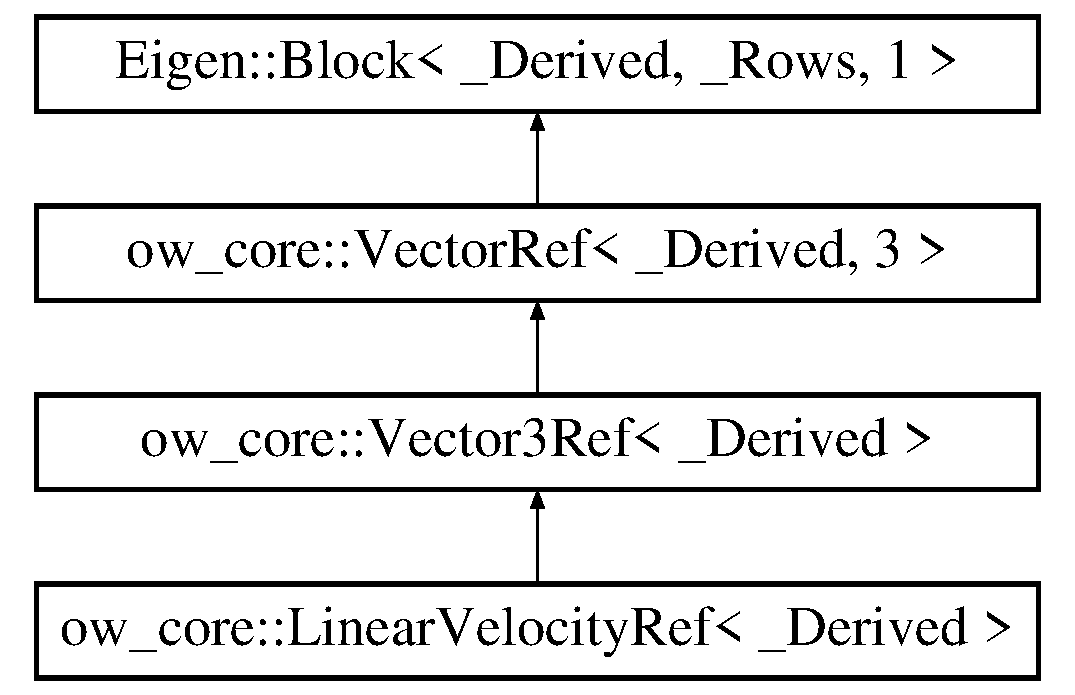
\includegraphics[height=4.000000cm]{d8/d79/classow__core_1_1LinearVelocityRef}
\end{center}
\end{figure}
\subsection*{Public Types}
\begin{DoxyCompactItemize}
\item 
typedef \+\_\+\+Derived {\bfseries Derived}\hypertarget{classow__core_1_1LinearVelocityRef_a3ac3012d274d4ac8eb2a40737e0b47a7}{}\label{classow__core_1_1LinearVelocityRef_a3ac3012d274d4ac8eb2a40737e0b47a7}

\item 
typedef \hyperlink{classow__core_1_1Vector3Ref}{Vector3\+Ref}$<$ Derived $>$ {\bfseries Base}\hypertarget{classow__core_1_1LinearVelocityRef_a1b6b82ecd607a6461d9b752c35cf1b98}{}\label{classow__core_1_1LinearVelocityRef_a1b6b82ecd607a6461d9b752c35cf1b98}

\end{DoxyCompactItemize}
\subsection*{Public Member Functions}
\begin{DoxyCompactItemize}
\item 
\hyperlink{classow__core_1_1LinearVelocityRef_a78f241cf9a1105b927f6f04ed6fa5d11}{Linear\+Velocity\+Ref} (Derived \&ref, int start\+Row=0, int start\+Col=0)
\begin{DoxyCompactList}\small\item\em Default Constructor. \end{DoxyCompactList}\end{DoxyCompactItemize}


\subsection{Detailed Description}
\subsubsection*{template$<$typename \+\_\+\+Derived$>$\\*
class ow\+\_\+core\+::\+Linear\+Velocity\+Ref$<$ \+\_\+\+Derived $>$}

The \hyperlink{classow__core_1_1LinearVelocityRef}{Linear\+Velocity\+Ref} class. 

The \hyperlink{classow__core_1_1LinearVelocityRef}{Linear\+Velocity\+Ref} is of type Eigen\+::\+Vector3 and is represented by the math symbol $\dot{\mathbf{x}}$.

References the data of another Eigen type class via Eigen\+::\+Block. 

\subsection{Constructor \& Destructor Documentation}
\index{ow\+\_\+core\+::\+Linear\+Velocity\+Ref@{ow\+\_\+core\+::\+Linear\+Velocity\+Ref}!Linear\+Velocity\+Ref@{Linear\+Velocity\+Ref}}
\index{Linear\+Velocity\+Ref@{Linear\+Velocity\+Ref}!ow\+\_\+core\+::\+Linear\+Velocity\+Ref@{ow\+\_\+core\+::\+Linear\+Velocity\+Ref}}
\subsubsection[{\texorpdfstring{Linear\+Velocity\+Ref(\+Derived \&ref, int start\+Row=0, int start\+Col=0)}{LinearVelocityRef(Derived &ref, int startRow=0, int startCol=0)}}]{\setlength{\rightskip}{0pt plus 5cm}template$<$typename \+\_\+\+Derived$>$ {\bf ow\+\_\+core\+::\+Linear\+Velocity\+Ref}$<$ \+\_\+\+Derived $>$\+::{\bf Linear\+Velocity\+Ref} (
\begin{DoxyParamCaption}
\item[{Derived \&}]{ref, }
\item[{int}]{start\+Row = {\ttfamily 0}, }
\item[{int}]{start\+Col = {\ttfamily 0}}
\end{DoxyParamCaption}
)\hspace{0.3cm}{\ttfamily [inline]}, {\ttfamily [explicit]}}\hypertarget{classow__core_1_1LinearVelocityRef_a78f241cf9a1105b927f6f04ed6fa5d11}{}\label{classow__core_1_1LinearVelocityRef_a78f241cf9a1105b927f6f04ed6fa5d11}


Default Constructor. 


\begin{DoxyParams}{Parameters}
{\em ref} & the reference to storage Eigen object to access the elements of the Linear\+Velocityn via Eigen\+::\+Block.\\
\hline
{\em start\+Row} & the start index of the row for Eigen\+::\+Block.\\
\hline
{\em start\+Col} & the start index of the column for Eigen\+::\+Block. \\
\hline
\end{DoxyParams}


The documentation for this class was generated from the following file\+:\begin{DoxyCompactItemize}
\item 
/home/dean/ros/workspaces/ow\+\_\+test\+\_\+ws/src/ow\+\_\+core/include/ow\+\_\+core/\hyperlink{linear__velocity__ref_8h}{linear\+\_\+velocity\+\_\+ref.\+h}\end{DoxyCompactItemize}

\hypertarget{classow__core_1_1MatrixRef}{}\section{ow\+\_\+core\+:\+:Matrix\+Ref$<$ \+\_\+\+Derived, \+\_\+\+Rows, \+\_\+\+Cols $>$ Class Template Reference}
\label{classow__core_1_1MatrixRef}\index{ow\+\_\+core\+::\+Matrix\+Ref$<$ \+\_\+\+Derived, \+\_\+\+Rows, \+\_\+\+Cols $>$@{ow\+\_\+core\+::\+Matrix\+Ref$<$ \+\_\+\+Derived, \+\_\+\+Rows, \+\_\+\+Cols $>$}}


The \hyperlink{classow__core_1_1MatrixRef}{Matrix\+Ref} class.  




{\ttfamily \#include $<$matrix\+\_\+ref.\+h$>$}

Inheritance diagram for ow\+\_\+core\+:\+:Matrix\+Ref$<$ \+\_\+\+Derived, \+\_\+\+Rows, \+\_\+\+Cols $>$\+:\begin{figure}[H]
\begin{center}
\leavevmode
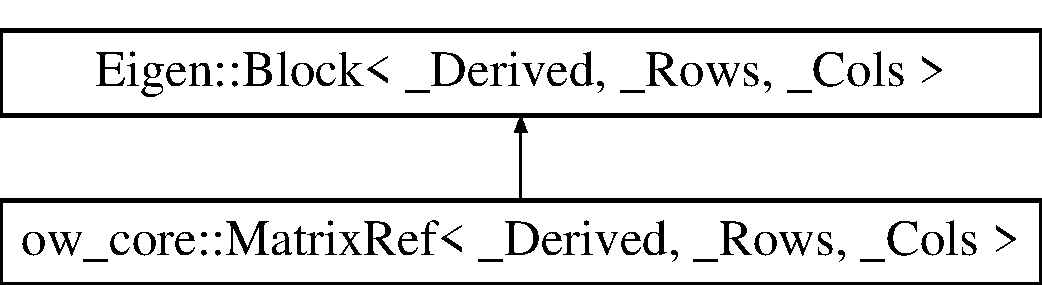
\includegraphics[height=2.000000cm]{df/dd7/classow__core_1_1MatrixRef}
\end{center}
\end{figure}
\subsection*{Public Types}
\begin{DoxyCompactItemize}
\item 
enum \{ {\bfseries Rows} = \+\_\+\+Rows, 
{\bfseries Cols} = \+\_\+\+Cols
 \}\hypertarget{classow__core_1_1MatrixRef_acbc53f5a50649a21caafebc91966f6d3}{}\label{classow__core_1_1MatrixRef_acbc53f5a50649a21caafebc91966f6d3}

\item 
typedef \+\_\+\+Derived {\bfseries Derived}\hypertarget{classow__core_1_1MatrixRef_ad0e55e853d08951e064718a8ac69ac96}{}\label{classow__core_1_1MatrixRef_ad0e55e853d08951e064718a8ac69ac96}

\item 
typedef Eigen\+::\+Block$<$ Derived, Rows, Cols $>$ {\bfseries Base}\hypertarget{classow__core_1_1MatrixRef_a2b935d9a0c707f1d2f709829413a75a4}{}\label{classow__core_1_1MatrixRef_a2b935d9a0c707f1d2f709829413a75a4}

\end{DoxyCompactItemize}
\subsection*{Public Member Functions}
\begin{DoxyCompactItemize}
\item 
\hyperlink{classow__core_1_1MatrixRef_aba4840a8e3d79c599a3390d6c64790af}{Matrix\+Ref} (Derived \&ref, int start\+Row=0, int start\+Col=0)
\begin{DoxyCompactList}\small\item\em Default Constructor. \end{DoxyCompactList}\item 
std\+::string \hyperlink{classow__core_1_1MatrixRef_af123840b0aeea5385866934a44998eef}{to\+String} () const 
\begin{DoxyCompactList}\small\item\em Conversion to std\+::string. \end{DoxyCompactList}\end{DoxyCompactItemize}


\subsection{Detailed Description}
\subsubsection*{template$<$typename \+\_\+\+Derived, int \+\_\+\+Rows, int \+\_\+\+Cols$>$\\*
class ow\+\_\+core\+::\+Matrix\+Ref$<$ \+\_\+\+Derived, \+\_\+\+Rows, \+\_\+\+Cols $>$}

The \hyperlink{classow__core_1_1MatrixRef}{Matrix\+Ref} class. 

References the data of another Eigen type class via Eigen\+:Block.

We need this special type to get the behavior of Eigen\+::\+Matrix when defining new references. 

\subsection{Constructor \& Destructor Documentation}
\index{ow\+\_\+core\+::\+Matrix\+Ref@{ow\+\_\+core\+::\+Matrix\+Ref}!Matrix\+Ref@{Matrix\+Ref}}
\index{Matrix\+Ref@{Matrix\+Ref}!ow\+\_\+core\+::\+Matrix\+Ref@{ow\+\_\+core\+::\+Matrix\+Ref}}
\subsubsection[{\texorpdfstring{Matrix\+Ref(\+Derived \&ref, int start\+Row=0, int start\+Col=0)}{MatrixRef(Derived &ref, int startRow=0, int startCol=0)}}]{\setlength{\rightskip}{0pt plus 5cm}template$<$typename \+\_\+\+Derived, int \+\_\+\+Rows, int \+\_\+\+Cols$>$ {\bf ow\+\_\+core\+::\+Matrix\+Ref}$<$ \+\_\+\+Derived, \+\_\+\+Rows, \+\_\+\+Cols $>$\+::{\bf Matrix\+Ref} (
\begin{DoxyParamCaption}
\item[{Derived \&}]{ref, }
\item[{int}]{start\+Row = {\ttfamily 0}, }
\item[{int}]{start\+Col = {\ttfamily 0}}
\end{DoxyParamCaption}
)\hspace{0.3cm}{\ttfamily [inline]}, {\ttfamily [explicit]}}\hypertarget{classow__core_1_1MatrixRef_aba4840a8e3d79c599a3390d6c64790af}{}\label{classow__core_1_1MatrixRef_aba4840a8e3d79c599a3390d6c64790af}


Default Constructor. 


\begin{DoxyParams}{Parameters}
{\em ref} & the reference to storage Eigen object to access the elements of the quaternion via Eigen\+::\+Block.\\
\hline
{\em start\+Row} & the start index of the row for Eigen\+::\+Block.\\
\hline
{\em start\+Col} & the start index of the column for Eigen\+::\+Block. \\
\hline
\end{DoxyParams}


\subsection{Member Function Documentation}
\index{ow\+\_\+core\+::\+Matrix\+Ref@{ow\+\_\+core\+::\+Matrix\+Ref}!to\+String@{to\+String}}
\index{to\+String@{to\+String}!ow\+\_\+core\+::\+Matrix\+Ref@{ow\+\_\+core\+::\+Matrix\+Ref}}
\subsubsection[{\texorpdfstring{to\+String() const }{toString() const }}]{\setlength{\rightskip}{0pt plus 5cm}template$<$typename \+\_\+\+Derived, int \+\_\+\+Rows, int \+\_\+\+Cols$>$ std\+::string {\bf ow\+\_\+core\+::\+Matrix\+Ref}$<$ \+\_\+\+Derived, \+\_\+\+Rows, \+\_\+\+Cols $>$\+::to\+String (
\begin{DoxyParamCaption}
{}
\end{DoxyParamCaption}
) const\hspace{0.3cm}{\ttfamily [inline]}}\hypertarget{classow__core_1_1MatrixRef_af123840b0aeea5385866934a44998eef}{}\label{classow__core_1_1MatrixRef_af123840b0aeea5385866934a44998eef}


Conversion to std\+::string. 

\begin{DoxyReturn}{Returns}
the string for this type. 
\end{DoxyReturn}


The documentation for this class was generated from the following file\+:\begin{DoxyCompactItemize}
\item 
/home/dean/ros/workspaces/ow\+\_\+test\+\_\+ws/src/ow\+\_\+core/include/ow\+\_\+core/\hyperlink{matrix__ref_8h}{matrix\+\_\+ref.\+h}\end{DoxyCompactItemize}

\hypertarget{classow__core_1_1Moment}{}\section{ow\+\_\+core\+:\+:Moment$<$ \+\_\+\+Scalar $>$ Class Template Reference}
\label{classow__core_1_1Moment}\index{ow\+\_\+core\+::\+Moment$<$ \+\_\+\+Scalar $>$@{ow\+\_\+core\+::\+Moment$<$ \+\_\+\+Scalar $>$}}


The \hyperlink{classow__core_1_1Moment}{Moment} class.  




{\ttfamily \#include $<$moment.\+h$>$}

Inheritance diagram for ow\+\_\+core\+:\+:Moment$<$ \+\_\+\+Scalar $>$\+:\begin{figure}[H]
\begin{center}
\leavevmode
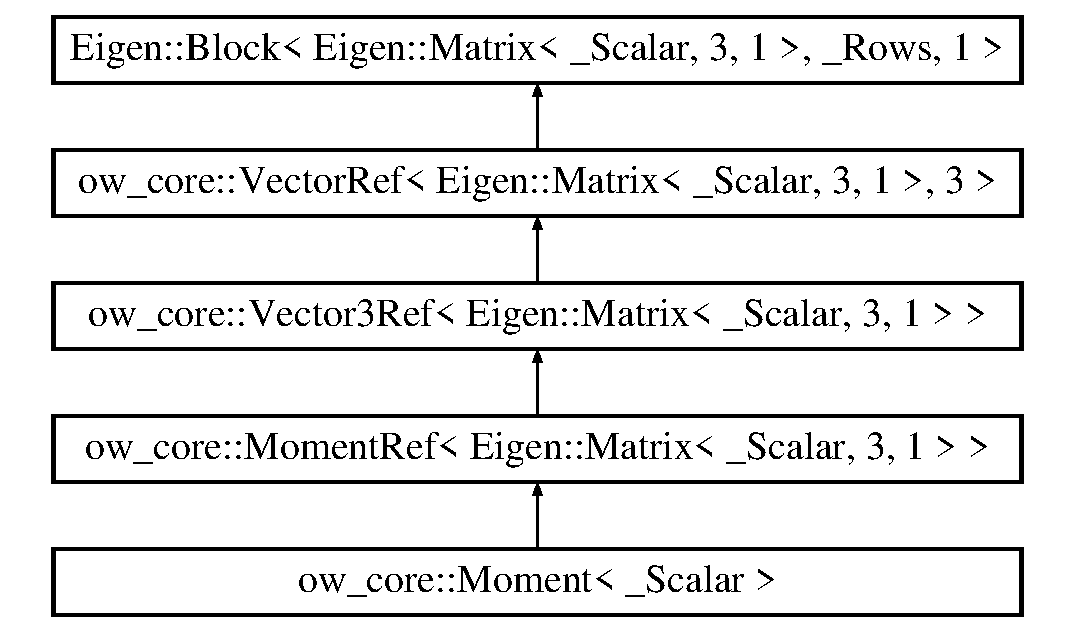
\includegraphics[height=5.000000cm]{da/d30/classow__core_1_1Moment}
\end{center}
\end{figure}
\subsection*{Public Types}
\begin{DoxyCompactItemize}
\item 
typedef \+\_\+\+Scalar {\bfseries Scalar}\hypertarget{classow__core_1_1Moment_a1b7a49145338008bf7346342cdda0549}{}\label{classow__core_1_1Moment_a1b7a49145338008bf7346342cdda0549}

\item 
typedef Eigen\+::\+Matrix$<$ \+\_\+\+Scalar, 3, 1 $>$ {\bfseries Derived}\hypertarget{classow__core_1_1Moment_a5974580adf3f59f807961230b8833cf8}{}\label{classow__core_1_1Moment_a5974580adf3f59f807961230b8833cf8}

\item 
typedef \hyperlink{classow__core_1_1MomentRef}{Moment\+Ref}$<$ Derived $>$ {\bfseries Base}\hypertarget{classow__core_1_1Moment_a858ac794296e7f501f7e25566b36dc44}{}\label{classow__core_1_1Moment_a858ac794296e7f501f7e25566b36dc44}

\end{DoxyCompactItemize}
\subsection*{Public Member Functions}
\begin{DoxyCompactItemize}
\item 
\hyperlink{classow__core_1_1Moment_ac0c0aa2da1fa194df0c4e32792f9bdb4}{Moment} ()\hypertarget{classow__core_1_1Moment_ac0c0aa2da1fa194df0c4e32792f9bdb4}{}\label{classow__core_1_1Moment_ac0c0aa2da1fa194df0c4e32792f9bdb4}

\begin{DoxyCompactList}\small\item\em Default Constructor. \end{DoxyCompactList}\item 
\hyperlink{classow__core_1_1Moment_a9c400630f5cd1bae41a68a4692138b96}{Moment} (const Scalar \&x, const Scalar \&y, const Scalar \&z)\hypertarget{classow__core_1_1Moment_a9c400630f5cd1bae41a68a4692138b96}{}\label{classow__core_1_1Moment_a9c400630f5cd1bae41a68a4692138b96}

\begin{DoxyCompactList}\small\item\em Assignment from Scalar values. \end{DoxyCompactList}\item 
{\footnotesize template$<$typename Other\+Derived $>$ }\\\hyperlink{classow__core_1_1Moment_a4e0a0f99a22ef5423718aae4db3b4935}{Moment} (const Eigen\+::\+Eigen\+Base$<$ Other\+Derived $>$ \&other)
\begin{DoxyCompactList}\small\item\em Copy constructor. \end{DoxyCompactList}\end{DoxyCompactItemize}
\subsection*{Protected Attributes}
\begin{DoxyCompactItemize}
\item 
Derived {\bfseries data\+\_\+}\hypertarget{classow__core_1_1Moment_afc9f0b1dc8468b83af5b84d96b039b9e}{}\label{classow__core_1_1Moment_afc9f0b1dc8468b83af5b84d96b039b9e}

\end{DoxyCompactItemize}


\subsection{Detailed Description}
\subsubsection*{template$<$typename \+\_\+\+Scalar$>$\\*
class ow\+\_\+core\+::\+Moment$<$ \+\_\+\+Scalar $>$}

The \hyperlink{classow__core_1_1Moment}{Moment} class. 

The \hyperlink{classow__core_1_1Moment}{Moment} is of type Eigen\+::\+Vector3 and is represented by the math symbol $\mathbf{\mu}$. 

\subsection{Constructor \& Destructor Documentation}
\index{ow\+\_\+core\+::\+Moment@{ow\+\_\+core\+::\+Moment}!Moment@{Moment}}
\index{Moment@{Moment}!ow\+\_\+core\+::\+Moment@{ow\+\_\+core\+::\+Moment}}
\subsubsection[{\texorpdfstring{Moment(const Eigen\+::\+Eigen\+Base$<$ Other\+Derived $>$ \&other)}{Moment(const Eigen::EigenBase< OtherDerived > &other)}}]{\setlength{\rightskip}{0pt plus 5cm}template$<$typename \+\_\+\+Scalar $>$ template$<$typename Other\+Derived $>$ {\bf ow\+\_\+core\+::\+Moment}$<$ \+\_\+\+Scalar $>$\+::{\bf Moment} (
\begin{DoxyParamCaption}
\item[{const Eigen\+::\+Eigen\+Base$<$ Other\+Derived $>$ \&}]{other}
\end{DoxyParamCaption}
)\hspace{0.3cm}{\ttfamily [inline]}}\hypertarget{classow__core_1_1Moment_a4e0a0f99a22ef5423718aae4db3b4935}{}\label{classow__core_1_1Moment_a4e0a0f99a22ef5423718aae4db3b4935}


Copy constructor. 

This copy constructor not only works with Eigen matrices but also with their expressions. 

The documentation for this class was generated from the following file\+:\begin{DoxyCompactItemize}
\item 
/home/dean/ros/workspaces/ow\+\_\+test\+\_\+ws/src/ow\+\_\+core/include/ow\+\_\+core/\hyperlink{moment_8h}{moment.\+h}\end{DoxyCompactItemize}

\hypertarget{classow__core_1_1MomentRef}{}\section{ow\+\_\+core\+:\+:Moment\+Ref$<$ \+\_\+\+Derived $>$ Class Template Reference}
\label{classow__core_1_1MomentRef}\index{ow\+\_\+core\+::\+Moment\+Ref$<$ \+\_\+\+Derived $>$@{ow\+\_\+core\+::\+Moment\+Ref$<$ \+\_\+\+Derived $>$}}


The \hyperlink{classow__core_1_1MomentRef}{Moment\+Ref} class.  




{\ttfamily \#include $<$moment\+\_\+ref.\+h$>$}

Inheritance diagram for ow\+\_\+core\+:\+:Moment\+Ref$<$ \+\_\+\+Derived $>$\+:\begin{figure}[H]
\begin{center}
\leavevmode
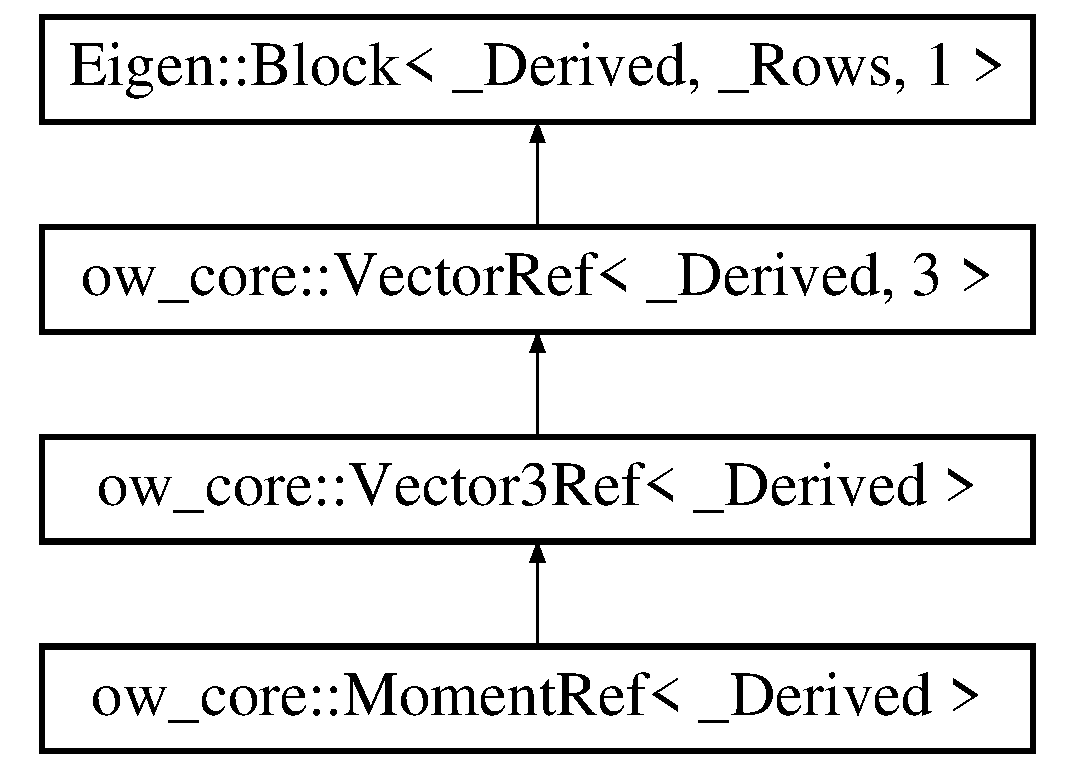
\includegraphics[height=4.000000cm]{de/d46/classow__core_1_1MomentRef}
\end{center}
\end{figure}
\subsection*{Public Types}
\begin{DoxyCompactItemize}
\item 
typedef \+\_\+\+Derived {\bfseries Derived}\hypertarget{classow__core_1_1MomentRef_a8381c7f3d2123c9d388b41dfa746f77d}{}\label{classow__core_1_1MomentRef_a8381c7f3d2123c9d388b41dfa746f77d}

\item 
typedef \hyperlink{classow__core_1_1Vector3Ref}{Vector3\+Ref}$<$ Derived $>$ {\bfseries Base}\hypertarget{classow__core_1_1MomentRef_a410591bc3879bc60e71b950e769bb031}{}\label{classow__core_1_1MomentRef_a410591bc3879bc60e71b950e769bb031}

\end{DoxyCompactItemize}
\subsection*{Public Member Functions}
\begin{DoxyCompactItemize}
\item 
\hyperlink{classow__core_1_1MomentRef_adafe9b697d0c0b3a2671e13680dfcd0f}{Moment\+Ref} (Derived \&ref, int start\+Row=0, int start\+Col=0)
\begin{DoxyCompactList}\small\item\em Default Constructor. \end{DoxyCompactList}\end{DoxyCompactItemize}


\subsection{Detailed Description}
\subsubsection*{template$<$typename \+\_\+\+Derived$>$\\*
class ow\+\_\+core\+::\+Moment\+Ref$<$ \+\_\+\+Derived $>$}

The \hyperlink{classow__core_1_1MomentRef}{Moment\+Ref} class. 

The \hyperlink{classow__core_1_1Moment}{Moment} is of type Eigen\+::\+Vector3 and is represented by the math symbol $\mathbf{\mu}$.

References the data of another Eigen type class via Eigen\+::\+Block. 

\subsection{Constructor \& Destructor Documentation}
\index{ow\+\_\+core\+::\+Moment\+Ref@{ow\+\_\+core\+::\+Moment\+Ref}!Moment\+Ref@{Moment\+Ref}}
\index{Moment\+Ref@{Moment\+Ref}!ow\+\_\+core\+::\+Moment\+Ref@{ow\+\_\+core\+::\+Moment\+Ref}}
\subsubsection[{\texorpdfstring{Moment\+Ref(\+Derived \&ref, int start\+Row=0, int start\+Col=0)}{MomentRef(Derived &ref, int startRow=0, int startCol=0)}}]{\setlength{\rightskip}{0pt plus 5cm}template$<$typename \+\_\+\+Derived$>$ {\bf ow\+\_\+core\+::\+Moment\+Ref}$<$ \+\_\+\+Derived $>$\+::{\bf Moment\+Ref} (
\begin{DoxyParamCaption}
\item[{Derived \&}]{ref, }
\item[{int}]{start\+Row = {\ttfamily 0}, }
\item[{int}]{start\+Col = {\ttfamily 0}}
\end{DoxyParamCaption}
)\hspace{0.3cm}{\ttfamily [inline]}, {\ttfamily [explicit]}}\hypertarget{classow__core_1_1MomentRef_adafe9b697d0c0b3a2671e13680dfcd0f}{}\label{classow__core_1_1MomentRef_adafe9b697d0c0b3a2671e13680dfcd0f}


Default Constructor. 


\begin{DoxyParams}{Parameters}
{\em ref} & the reference to storage Eigen object to access the elements of the Linear\+Velocityn via Eigen\+::\+Block.\\
\hline
{\em start\+Row} & the start index of the row for Eigen\+::\+Block.\\
\hline
{\em start\+Col} & the start index of the column for Eigen\+::\+Block. \\
\hline
\end{DoxyParams}


The documentation for this class was generated from the following file\+:\begin{DoxyCompactItemize}
\item 
/home/dean/ros/workspaces/ow\+\_\+test\+\_\+ws/src/ow\+\_\+core/include/ow\+\_\+core/\hyperlink{moment__ref_8h}{moment\+\_\+ref.\+h}\end{DoxyCompactItemize}

\hypertarget{classow__core_1_1QuaternionRef}{}\section{ow\+\_\+core\+:\+:Quaternion\+Ref$<$ \+\_\+\+Derived $>$ Class Template Reference}
\label{classow__core_1_1QuaternionRef}\index{ow\+\_\+core\+::\+Quaternion\+Ref$<$ \+\_\+\+Derived $>$@{ow\+\_\+core\+::\+Quaternion\+Ref$<$ \+\_\+\+Derived $>$}}


Get \hyperlink{classEigen_1_1QuaternionRef}{Eigen\+::\+Quaternion\+Ref} to our namespace.  




{\ttfamily \#include $<$quaternion\+\_\+ref.\+h$>$}

Inheritance diagram for ow\+\_\+core\+:\+:Quaternion\+Ref$<$ \+\_\+\+Derived $>$\+:\begin{figure}[H]
\begin{center}
\leavevmode
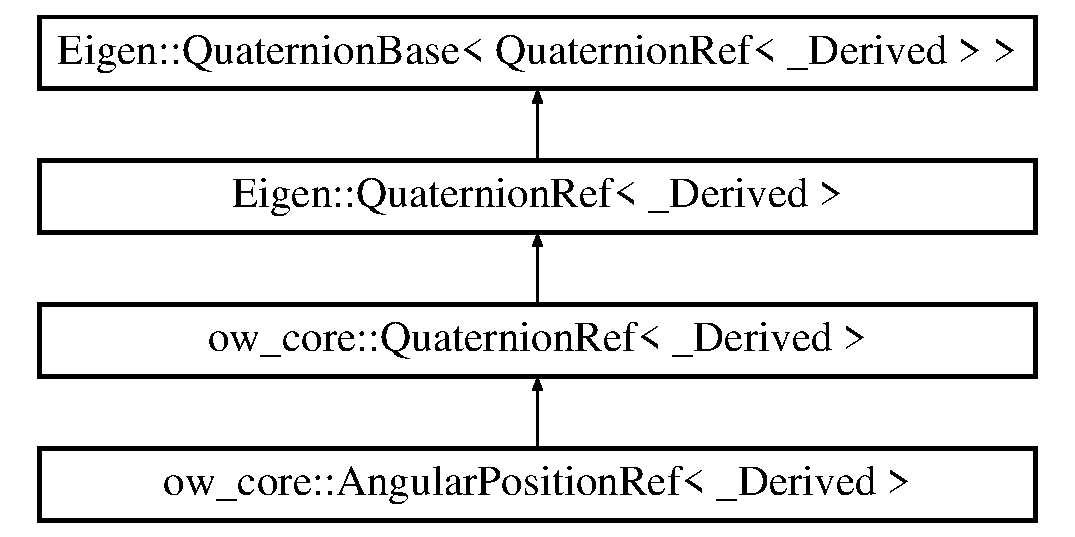
\includegraphics[height=4.000000cm]{d8/dae/classow__core_1_1QuaternionRef}
\end{center}
\end{figure}
\subsection*{Public Types}
\begin{DoxyCompactItemize}
\item 
typedef \+\_\+\+Derived {\bfseries Derived}\hypertarget{classow__core_1_1QuaternionRef_a0a3fe2b7030b00914878ab4ad65faa1d}{}\label{classow__core_1_1QuaternionRef_a0a3fe2b7030b00914878ab4ad65faa1d}

\item 
typedef \hyperlink{classEigen_1_1QuaternionRef}{Eigen\+::\+Quaternion\+Ref}$<$ Derived $>$ {\bfseries Base}\hypertarget{classow__core_1_1QuaternionRef_a3beee92d95baf28e734df3ef3a795fb5}{}\label{classow__core_1_1QuaternionRef_a3beee92d95baf28e734df3ef3a795fb5}

\end{DoxyCompactItemize}
\subsection*{Public Member Functions}
\begin{DoxyCompactItemize}
\item 
\hyperlink{classow__core_1_1QuaternionRef_a7752f6e95ec9704285d1c5fc5d7ba2ee}{Quaternion\+Ref} (Derived \&ref, int start\+Row=0, int start\+Col=0)
\begin{DoxyCompactList}\small\item\em Default Constructor. \end{DoxyCompactList}\end{DoxyCompactItemize}
\subsection*{Additional Inherited Members}


\subsection{Detailed Description}
\subsubsection*{template$<$typename \+\_\+\+Derived$>$\\*
class ow\+\_\+core\+::\+Quaternion\+Ref$<$ \+\_\+\+Derived $>$}

Get \hyperlink{classEigen_1_1QuaternionRef}{Eigen\+::\+Quaternion\+Ref} to our namespace. 

The \hyperlink{classow__core_1_1QuaternionRef}{Quaternion\+Ref} class.

References the data of another Eigen type class via Eigen\+:Block.

We need this special type to get the behavior of Eigen\+::\+Quaternion when defining new references. 

\subsection{Constructor \& Destructor Documentation}
\index{ow\+\_\+core\+::\+Quaternion\+Ref@{ow\+\_\+core\+::\+Quaternion\+Ref}!Quaternion\+Ref@{Quaternion\+Ref}}
\index{Quaternion\+Ref@{Quaternion\+Ref}!ow\+\_\+core\+::\+Quaternion\+Ref@{ow\+\_\+core\+::\+Quaternion\+Ref}}
\subsubsection[{\texorpdfstring{Quaternion\+Ref(\+Derived \&ref, int start\+Row=0, int start\+Col=0)}{QuaternionRef(Derived &ref, int startRow=0, int startCol=0)}}]{\setlength{\rightskip}{0pt plus 5cm}template$<$typename \+\_\+\+Derived$>$ {\bf ow\+\_\+core\+::\+Quaternion\+Ref}$<$ \+\_\+\+Derived $>$\+::{\bf Quaternion\+Ref} (
\begin{DoxyParamCaption}
\item[{Derived \&}]{ref, }
\item[{int}]{start\+Row = {\ttfamily 0}, }
\item[{int}]{start\+Col = {\ttfamily 0}}
\end{DoxyParamCaption}
)\hspace{0.3cm}{\ttfamily [inline]}}\hypertarget{classow__core_1_1QuaternionRef_a7752f6e95ec9704285d1c5fc5d7ba2ee}{}\label{classow__core_1_1QuaternionRef_a7752f6e95ec9704285d1c5fc5d7ba2ee}


Default Constructor. 


\begin{DoxyParams}{Parameters}
{\em ref} & the reference to storage Eigen object to access the elements of the quaternion via Eigen\+::\+Block.\\
\hline
{\em start\+Row} & the start index of the row for Eigen\+::\+Block.\\
\hline
{\em start\+Col} & the start index of the column for Eigen\+::\+Block. \\
\hline
\end{DoxyParams}


The documentation for this class was generated from the following file\+:\begin{DoxyCompactItemize}
\item 
/home/dean/ros/workspaces/ow\+\_\+test\+\_\+ws/src/ow\+\_\+core/include/ow\+\_\+core/\hyperlink{quaternion__ref_8h}{quaternion\+\_\+ref.\+h}\end{DoxyCompactItemize}

\hypertarget{classEigen_1_1QuaternionRef}{}\section{Eigen\+:\+:Quaternion\+Ref$<$ \+\_\+\+Derived $>$ Class Template Reference}
\label{classEigen_1_1QuaternionRef}\index{Eigen\+::\+Quaternion\+Ref$<$ \+\_\+\+Derived $>$@{Eigen\+::\+Quaternion\+Ref$<$ \+\_\+\+Derived $>$}}


The \hyperlink{classEigen_1_1QuaternionRef}{Quaternion\+Ref} class.  




{\ttfamily \#include $<$quaternion\+\_\+ref.\+h$>$}

Inheritance diagram for Eigen\+:\+:Quaternion\+Ref$<$ \+\_\+\+Derived $>$\+:\begin{figure}[H]
\begin{center}
\leavevmode
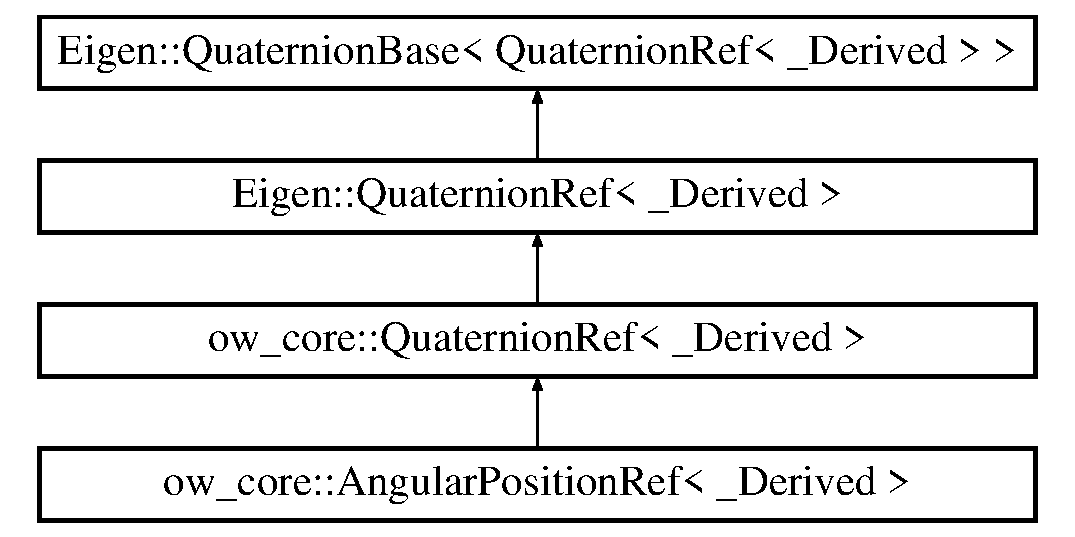
\includegraphics[height=4.000000cm]{d7/d7b/classEigen_1_1QuaternionRef}
\end{center}
\end{figure}
\subsection*{Public Types}
\begin{DoxyCompactItemize}
\item 
typedef \+\_\+\+Derived {\bfseries Derived}\hypertarget{classEigen_1_1QuaternionRef_ae01d4bb6ac378f260ed60b076cadf7e8}{}\label{classEigen_1_1QuaternionRef_ae01d4bb6ac378f260ed60b076cadf7e8}

\item 
typedef Eigen\+::\+Quaternion\+Base$<$ \hyperlink{classEigen_1_1QuaternionRef}{Quaternion\+Ref}$<$ \+\_\+\+Derived $>$ $>$ {\bfseries Base}\hypertarget{classEigen_1_1QuaternionRef_a4eb09c1c2266a2a7d36fe6a8d9bd1f44}{}\label{classEigen_1_1QuaternionRef_a4eb09c1c2266a2a7d36fe6a8d9bd1f44}

\item 
typedef Eigen\+::internal\+::traits$<$ \hyperlink{classEigen_1_1QuaternionRef}{Quaternion\+Ref} $>$\+::Coefficients {\bfseries Coefficients}\hypertarget{classEigen_1_1QuaternionRef_a5f3aa5e5a4749058a47b2c491fc8adde}{}\label{classEigen_1_1QuaternionRef_a5f3aa5e5a4749058a47b2c491fc8adde}

\end{DoxyCompactItemize}
\subsection*{Public Member Functions}
\begin{DoxyCompactItemize}
\item 
\hyperlink{classEigen_1_1QuaternionRef_a248478189cea730141b0a3b9d9dd9a63}{Quaternion\+Ref} (Derived \&ref, int start\+Row=0, int start\+Col=0)
\begin{DoxyCompactList}\small\item\em Default Constructor. \end{DoxyCompactList}\item 
Coefficients \& \hyperlink{classEigen_1_1QuaternionRef_ad181c3d0f58e30e4508c10f7c6bc8c73}{coeffs} ()
\begin{DoxyCompactList}\small\item\em Get quaternion coefficients. \end{DoxyCompactList}\item 
const Coefficients \& \hyperlink{classEigen_1_1QuaternionRef_a32775ef17d906112484443a31307052f}{coeffs} () const 
\begin{DoxyCompactList}\small\item\em Get quaternion coefficients. \end{DoxyCompactList}\item 
std\+::string \hyperlink{classEigen_1_1QuaternionRef_a29a95c2bb2683a0720d7b0e55a79ef56}{to\+String} () const \hypertarget{classEigen_1_1QuaternionRef_a29a95c2bb2683a0720d7b0e55a79ef56}{}\label{classEigen_1_1QuaternionRef_a29a95c2bb2683a0720d7b0e55a79ef56}

\begin{DoxyCompactList}\small\item\em Conversion to std\+::string. \end{DoxyCompactList}\end{DoxyCompactItemize}
\subsection*{Protected Attributes}
\begin{DoxyCompactItemize}
\item 
Coefficients \hyperlink{classEigen_1_1QuaternionRef_a236621f8f2822fc2c9ef50069badf64f}{coeffs\+\_\+}\hypertarget{classEigen_1_1QuaternionRef_a236621f8f2822fc2c9ef50069badf64f}{}\label{classEigen_1_1QuaternionRef_a236621f8f2822fc2c9ef50069badf64f}

\begin{DoxyCompactList}\small\item\em The quaternion coefficients in a Eigen\+::\+Block. \end{DoxyCompactList}\end{DoxyCompactItemize}


\subsection{Detailed Description}
\subsubsection*{template$<$typename \+\_\+\+Derived$>$\\*
class Eigen\+::\+Quaternion\+Ref$<$ \+\_\+\+Derived $>$}

The \hyperlink{classEigen_1_1QuaternionRef}{Quaternion\+Ref} class. 

This class provides access to the quaternion elements within another Eigen type class. This Eigen type class has to provide/support the Eigen\+::\+Block access.

We need this special type to get the behavior of Eigen\+::\+Quaternion in references where the source of the Quaternion elements is not a Quaternion itsself. 

\subsection{Constructor \& Destructor Documentation}
\index{Eigen\+::\+Quaternion\+Ref@{Eigen\+::\+Quaternion\+Ref}!Quaternion\+Ref@{Quaternion\+Ref}}
\index{Quaternion\+Ref@{Quaternion\+Ref}!Eigen\+::\+Quaternion\+Ref@{Eigen\+::\+Quaternion\+Ref}}
\subsubsection[{\texorpdfstring{Quaternion\+Ref(\+Derived \&ref, int start\+Row=0, int start\+Col=0)}{QuaternionRef(Derived &ref, int startRow=0, int startCol=0)}}]{\setlength{\rightskip}{0pt plus 5cm}template$<$typename \+\_\+\+Derived$>$ {\bf Eigen\+::\+Quaternion\+Ref}$<$ \+\_\+\+Derived $>$\+::{\bf Quaternion\+Ref} (
\begin{DoxyParamCaption}
\item[{Derived \&}]{ref, }
\item[{int}]{start\+Row = {\ttfamily 0}, }
\item[{int}]{start\+Col = {\ttfamily 0}}
\end{DoxyParamCaption}
)\hspace{0.3cm}{\ttfamily [inline]}}\hypertarget{classEigen_1_1QuaternionRef_a248478189cea730141b0a3b9d9dd9a63}{}\label{classEigen_1_1QuaternionRef_a248478189cea730141b0a3b9d9dd9a63}


Default Constructor. 


\begin{DoxyParams}{Parameters}
{\em ref} & the reference to storage Eigen object to access the elements of the quaternion via Eigen\+::\+Block.\\
\hline
{\em start\+Row} & the start index of the row for Eigen\+::\+Block.\\
\hline
{\em start\+Col} & the start index of the column for Eigen\+::\+Block. \\
\hline
\end{DoxyParams}


\subsection{Member Function Documentation}
\index{Eigen\+::\+Quaternion\+Ref@{Eigen\+::\+Quaternion\+Ref}!coeffs@{coeffs}}
\index{coeffs@{coeffs}!Eigen\+::\+Quaternion\+Ref@{Eigen\+::\+Quaternion\+Ref}}
\subsubsection[{\texorpdfstring{coeffs()}{coeffs()}}]{\setlength{\rightskip}{0pt plus 5cm}template$<$typename \+\_\+\+Derived$>$ Coefficients\& {\bf Eigen\+::\+Quaternion\+Ref}$<$ \+\_\+\+Derived $>$\+::coeffs (
\begin{DoxyParamCaption}
{}
\end{DoxyParamCaption}
)\hspace{0.3cm}{\ttfamily [inline]}}\hypertarget{classEigen_1_1QuaternionRef_ad181c3d0f58e30e4508c10f7c6bc8c73}{}\label{classEigen_1_1QuaternionRef_ad181c3d0f58e30e4508c10f7c6bc8c73}


Get quaternion coefficients. 

This function is used internally by Eigen to get the coefficients for the Quaternion functionalities provided by Eigen\+::\+Quaternion\+Base. \index{Eigen\+::\+Quaternion\+Ref@{Eigen\+::\+Quaternion\+Ref}!coeffs@{coeffs}}
\index{coeffs@{coeffs}!Eigen\+::\+Quaternion\+Ref@{Eigen\+::\+Quaternion\+Ref}}
\subsubsection[{\texorpdfstring{coeffs() const }{coeffs() const }}]{\setlength{\rightskip}{0pt plus 5cm}template$<$typename \+\_\+\+Derived$>$ const Coefficients\& {\bf Eigen\+::\+Quaternion\+Ref}$<$ \+\_\+\+Derived $>$\+::coeffs (
\begin{DoxyParamCaption}
{}
\end{DoxyParamCaption}
) const\hspace{0.3cm}{\ttfamily [inline]}}\hypertarget{classEigen_1_1QuaternionRef_a32775ef17d906112484443a31307052f}{}\label{classEigen_1_1QuaternionRef_a32775ef17d906112484443a31307052f}


Get quaternion coefficients. 

This function is used internally by Eigen to get the coefficients for the Quaternion functionalities provided by Eigen\+::\+Quaternion\+Base. 

The documentation for this class was generated from the following file\+:\begin{DoxyCompactItemize}
\item 
/home/dean/ros/workspaces/ow\+\_\+test\+\_\+ws/src/ow\+\_\+core/include/ow\+\_\+core/\+Eigen/\hyperlink{Eigen_2quaternion__ref_8h}{quaternion\+\_\+ref.\+h}\end{DoxyCompactItemize}

\hypertarget{classow__core_1_1RobotOutPorts}{}\section{ow\+\_\+core\+:\+:Robot\+Out\+Ports Class Reference}
\label{classow__core_1_1RobotOutPorts}\index{ow\+\_\+core\+::\+Robot\+Out\+Ports@{ow\+\_\+core\+::\+Robot\+Out\+Ports}}


The \hyperlink{classow__core_1_1RobotOutPorts}{Robot\+Out\+Ports} class.  




{\ttfamily \#include $<$robot\+\_\+out\+\_\+ports.\+h$>$}

Inheritance diagram for ow\+\_\+core\+:\+:Robot\+Out\+Ports\+:\begin{figure}[H]
\begin{center}
\leavevmode
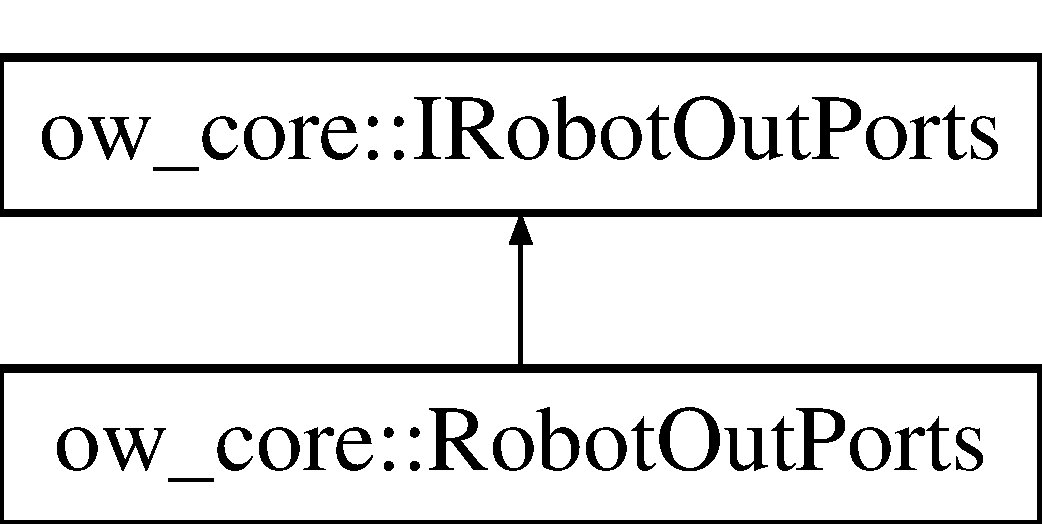
\includegraphics[height=2.000000cm]{d4/d2e/classow__core_1_1RobotOutPorts}
\end{center}
\end{figure}
\subsection*{Public Member Functions}
\begin{DoxyCompactItemize}
\item 
virtual \hyperlink{classow__core_1_1RobotOutPorts_aed43bf186fbc8bac85e9dd4896d696da}{$\sim$\+Robot\+Out\+Ports} ()\hypertarget{classow__core_1_1RobotOutPorts_aed43bf186fbc8bac85e9dd4896d696da}{}\label{classow__core_1_1RobotOutPorts_aed43bf186fbc8bac85e9dd4896d696da}

\begin{DoxyCompactList}\small\item\em Virtual destructor. \end{DoxyCompactList}\item 
virtual \hyperlink{classow__core_1_1IRobotOutPortsReal}{I\+Robot\+Out\+Ports\+Real} $\ast$ {\bfseries real} ()\hypertarget{classow__core_1_1RobotOutPorts_a519248bb84f2eca7ab681c5886c5b4ff}{}\label{classow__core_1_1RobotOutPorts_a519248bb84f2eca7ab681c5886c5b4ff}

\item 
virtual const \hyperlink{classow__core_1_1IRobotOutPortsReal}{I\+Robot\+Out\+Ports\+Real} $\ast$ {\bfseries real} () const \hypertarget{classow__core_1_1RobotOutPorts_a3149b8a0c58d40d0908ddf509d950165}{}\label{classow__core_1_1RobotOutPorts_a3149b8a0c58d40d0908ddf509d950165}

\item 
virtual \hyperlink{classow__core_1_1IRobotOutPortsCmd}{I\+Robot\+Out\+Ports\+Cmd} $\ast$ {\bfseries cmd} ()\hypertarget{classow__core_1_1RobotOutPorts_a398fa2e0702ec1cf92ce6b1b7ea8c919}{}\label{classow__core_1_1RobotOutPorts_a398fa2e0702ec1cf92ce6b1b7ea8c919}

\item 
virtual const \hyperlink{classow__core_1_1IRobotOutPortsCmd}{I\+Robot\+Out\+Ports\+Cmd} $\ast$ {\bfseries cmd} () const \hypertarget{classow__core_1_1RobotOutPorts_a33022afaf079177e3b4ec826c6581b29}{}\label{classow__core_1_1RobotOutPorts_a33022afaf079177e3b4ec826c6581b29}

\end{DoxyCompactItemize}
\subsection*{Protected Attributes}
\begin{DoxyCompactItemize}
\item 
\hyperlink{classow__core_1_1RobotOutPortsReal}{ow\+\_\+core\+::\+Robot\+Out\+Ports\+Real} {\bfseries real\+\_\+}\hypertarget{classow__core_1_1RobotOutPorts_ac4ee9ca0cdfbeb8046927dd09f34a8cd}{}\label{classow__core_1_1RobotOutPorts_ac4ee9ca0cdfbeb8046927dd09f34a8cd}

\item 
\hyperlink{classow__core_1_1RobotOutPortsCmd}{ow\+\_\+core\+::\+Robot\+Out\+Ports\+Cmd} {\bfseries cmd\+\_\+}\hypertarget{classow__core_1_1RobotOutPorts_a8b231e38fe976394b75872183edb447a}{}\label{classow__core_1_1RobotOutPorts_a8b231e38fe976394b75872183edb447a}

\end{DoxyCompactItemize}


\subsection{Detailed Description}
The \hyperlink{classow__core_1_1RobotOutPorts}{Robot\+Out\+Ports} class. 

The default implementation of the \hyperlink{classow__core_1_1RobotOutPorts}{Robot\+Out\+Ports} interface. 

The documentation for this class was generated from the following file\+:\begin{DoxyCompactItemize}
\item 
/home/dean/ros/workspaces/ow\+\_\+test\+\_\+ws/src/ow\+\_\+core/include/ow\+\_\+core/\+Implementations/\hyperlink{robot__out__ports_8h}{robot\+\_\+out\+\_\+ports.\+h}\end{DoxyCompactItemize}

\hypertarget{classow__core_1_1RobotOutPortsCmd}{}\section{ow\+\_\+core\+:\+:Robot\+Out\+Ports\+Cmd Class Reference}
\label{classow__core_1_1RobotOutPortsCmd}\index{ow\+\_\+core\+::\+Robot\+Out\+Ports\+Cmd@{ow\+\_\+core\+::\+Robot\+Out\+Ports\+Cmd}}


The \hyperlink{classow__core_1_1RobotOutPortsCmd}{Robot\+Out\+Ports\+Cmd} class.  




{\ttfamily \#include $<$robot\+\_\+out\+\_\+ports\+\_\+cmd.\+h$>$}

Inheritance diagram for ow\+\_\+core\+:\+:Robot\+Out\+Ports\+Cmd\+:\begin{figure}[H]
\begin{center}
\leavevmode
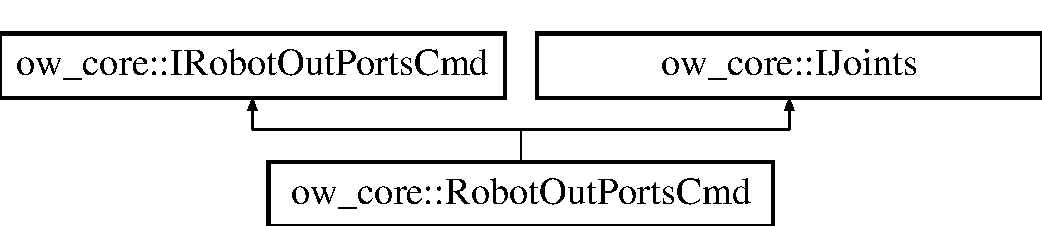
\includegraphics[height=2.000000cm]{db/de7/classow__core_1_1RobotOutPortsCmd}
\end{center}
\end{figure}
\subsection*{Public Member Functions}
\begin{DoxyCompactItemize}
\item 
virtual \hyperlink{classow__core_1_1RobotOutPortsCmd_ad018ac0a0a8c73aaf7bc62f7b28a0268}{$\sim$\+Robot\+Out\+Ports\+Cmd} ()\hypertarget{classow__core_1_1RobotOutPortsCmd_ad018ac0a0a8c73aaf7bc62f7b28a0268}{}\label{classow__core_1_1RobotOutPortsCmd_ad018ac0a0a8c73aaf7bc62f7b28a0268}

\begin{DoxyCompactList}\small\item\em Virtual destructor. \end{DoxyCompactList}\item 
virtual \hyperlink{classow__core_1_1IJoints}{I\+Joints} $\ast$ {\bfseries joints} ()\hypertarget{classow__core_1_1RobotOutPortsCmd_afb61fc492e221bfa994cf13c2ed92df6}{}\label{classow__core_1_1RobotOutPortsCmd_afb61fc492e221bfa994cf13c2ed92df6}

\item 
virtual const \hyperlink{classow__core_1_1IJoints}{I\+Joints} $\ast$ {\bfseries joints} () const \hypertarget{classow__core_1_1RobotOutPortsCmd_ad28a8aa922b9edf3815e016bbade0678}{}\label{classow__core_1_1RobotOutPortsCmd_ad28a8aa922b9edf3815e016bbade0678}

\item 
virtual \hyperlink{classow__core_1_1JointState}{ow\+::\+Joint\+State} \& {\bfseries joint\+State} ()\hypertarget{classow__core_1_1RobotOutPortsCmd_a4ea1c3b05b424d5c286d41ef73abca6f}{}\label{classow__core_1_1RobotOutPortsCmd_a4ea1c3b05b424d5c286d41ef73abca6f}

\item 
virtual const \hyperlink{classow__core_1_1JointState}{ow\+::\+Joint\+State} \& {\bfseries joint\+State} () const \hypertarget{classow__core_1_1RobotOutPortsCmd_a29242a677dca4a3c0a1f0ea74d088fc6}{}\label{classow__core_1_1RobotOutPortsCmd_a29242a677dca4a3c0a1f0ea74d088fc6}

\end{DoxyCompactItemize}
\subsection*{Protected Attributes}
\begin{DoxyCompactItemize}
\item 
\hyperlink{classow__core_1_1JointState}{ow\+::\+Joint\+State} {\bfseries js\+\_\+}\hypertarget{classow__core_1_1RobotOutPortsCmd_aece9d52a653226289b960d1a421fadc7}{}\label{classow__core_1_1RobotOutPortsCmd_aece9d52a653226289b960d1a421fadc7}

\end{DoxyCompactItemize}


\subsection{Detailed Description}
The \hyperlink{classow__core_1_1RobotOutPortsCmd}{Robot\+Out\+Ports\+Cmd} class. 

The default implementation of the \hyperlink{classow__core_1_1RobotOutPortsCmd}{Robot\+Out\+Ports\+Cmd} interface. 

The documentation for this class was generated from the following file\+:\begin{DoxyCompactItemize}
\item 
/home/dean/ros/workspaces/ow\+\_\+test\+\_\+ws/src/ow\+\_\+core/include/ow\+\_\+core/\+Implementations/\hyperlink{robot__out__ports__cmd_8h}{robot\+\_\+out\+\_\+ports\+\_\+cmd.\+h}\end{DoxyCompactItemize}

\hypertarget{classow__core_1_1RobotOutPortsReal}{}\section{ow\+\_\+core\+:\+:Robot\+Out\+Ports\+Real Class Reference}
\label{classow__core_1_1RobotOutPortsReal}\index{ow\+\_\+core\+::\+Robot\+Out\+Ports\+Real@{ow\+\_\+core\+::\+Robot\+Out\+Ports\+Real}}


The \hyperlink{classow__core_1_1RobotOutPortsReal}{Robot\+Out\+Ports\+Real} class.  




{\ttfamily \#include $<$robot\+\_\+out\+\_\+ports\+\_\+real.\+h$>$}

Inheritance diagram for ow\+\_\+core\+:\+:Robot\+Out\+Ports\+Real\+:\begin{figure}[H]
\begin{center}
\leavevmode
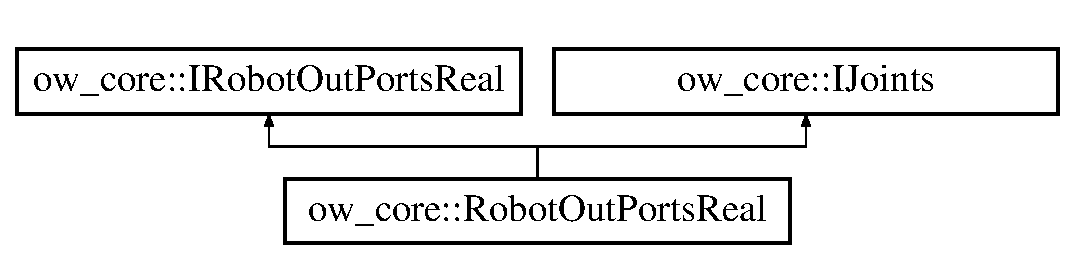
\includegraphics[height=2.000000cm]{df/db5/classow__core_1_1RobotOutPortsReal}
\end{center}
\end{figure}
\subsection*{Public Member Functions}
\begin{DoxyCompactItemize}
\item 
virtual \hyperlink{classow__core_1_1RobotOutPortsReal_a39f2fa114f429a749eb51dc52216552f}{$\sim$\+Robot\+Out\+Ports\+Real} ()\hypertarget{classow__core_1_1RobotOutPortsReal_a39f2fa114f429a749eb51dc52216552f}{}\label{classow__core_1_1RobotOutPortsReal_a39f2fa114f429a749eb51dc52216552f}

\begin{DoxyCompactList}\small\item\em Virtual destructor. \end{DoxyCompactList}\item 
virtual \hyperlink{classow__core_1_1IImuSensor}{I\+Imu\+Sensor} $\ast$ {\bfseries imu\+Sensor} ()\hypertarget{classow__core_1_1RobotOutPortsReal_afff66144f7d22f7c649713d5e60cd1c5}{}\label{classow__core_1_1RobotOutPortsReal_afff66144f7d22f7c649713d5e60cd1c5}

\item 
virtual const \hyperlink{classow__core_1_1IImuSensor}{I\+Imu\+Sensor} $\ast$ {\bfseries imu\+Sensor} () const \hypertarget{classow__core_1_1RobotOutPortsReal_a22f44cd9c847612acaacfc7396dff64b}{}\label{classow__core_1_1RobotOutPortsReal_a22f44cd9c847612acaacfc7396dff64b}

\item 
virtual \hyperlink{classow__core_1_1IForceTorqueSensors}{I\+Force\+Torque\+Sensors} $\ast$ {\bfseries force\+Torque\+Sensors} ()\hypertarget{classow__core_1_1RobotOutPortsReal_a5f4efdea4e27e18a0fc07a733a472372}{}\label{classow__core_1_1RobotOutPortsReal_a5f4efdea4e27e18a0fc07a733a472372}

\item 
virtual const \hyperlink{classow__core_1_1IForceTorqueSensors}{I\+Force\+Torque\+Sensors} $\ast$ {\bfseries force\+Torque\+Sensors} () const \hypertarget{classow__core_1_1RobotOutPortsReal_a48544ac0f33960465363fb8eb3bbb0c9}{}\label{classow__core_1_1RobotOutPortsReal_a48544ac0f33960465363fb8eb3bbb0c9}

\item 
virtual \hyperlink{classow__core_1_1IJoints}{I\+Joints} $\ast$ {\bfseries joints} ()\hypertarget{classow__core_1_1RobotOutPortsReal_aaed7004404fb7b926e9dffa5d097659f}{}\label{classow__core_1_1RobotOutPortsReal_aaed7004404fb7b926e9dffa5d097659f}

\item 
virtual const \hyperlink{classow__core_1_1IJoints}{I\+Joints} $\ast$ {\bfseries joints} () const \hypertarget{classow__core_1_1RobotOutPortsReal_a8df6cdf2b917c01630d7eafbe5c3f9df}{}\label{classow__core_1_1RobotOutPortsReal_a8df6cdf2b917c01630d7eafbe5c3f9df}

\item 
virtual \hyperlink{classow__core_1_1JointState}{ow\+::\+Joint\+State} \& {\bfseries joint\+State} ()\hypertarget{classow__core_1_1RobotOutPortsReal_aa83eb2299031d87be7dd88a43f9d2e84}{}\label{classow__core_1_1RobotOutPortsReal_aa83eb2299031d87be7dd88a43f9d2e84}

\item 
virtual const \hyperlink{classow__core_1_1JointState}{ow\+::\+Joint\+State} \& {\bfseries joint\+State} () const \hypertarget{classow__core_1_1RobotOutPortsReal_ab38ad9e62a901c95cccd63d9a6f28c5b}{}\label{classow__core_1_1RobotOutPortsReal_ab38ad9e62a901c95cccd63d9a6f28c5b}

\end{DoxyCompactItemize}
\subsection*{Protected Attributes}
\begin{DoxyCompactItemize}
\item 
\hyperlink{classow__core_1_1ImuSensor}{ow\+\_\+core\+::\+Imu\+Sensor} {\bfseries imu\+\_\+}\hypertarget{classow__core_1_1RobotOutPortsReal_a4eaac66c91f5464eb1b08e294c692732}{}\label{classow__core_1_1RobotOutPortsReal_a4eaac66c91f5464eb1b08e294c692732}

\item 
\hyperlink{classow__core_1_1ForceTorqueSensors}{ow\+\_\+core\+::\+Force\+Torque\+Sensors} {\bfseries fts\+\_\+}\hypertarget{classow__core_1_1RobotOutPortsReal_a69818c3bd63c8546528d0b14c6155de0}{}\label{classow__core_1_1RobotOutPortsReal_a69818c3bd63c8546528d0b14c6155de0}

\item 
\hyperlink{classow__core_1_1JointState}{ow\+::\+Joint\+State} {\bfseries js\+\_\+}\hypertarget{classow__core_1_1RobotOutPortsReal_affd22401b69ff18267dc4cc6383dc769}{}\label{classow__core_1_1RobotOutPortsReal_affd22401b69ff18267dc4cc6383dc769}

\end{DoxyCompactItemize}


\subsection{Detailed Description}
The \hyperlink{classow__core_1_1RobotOutPortsReal}{Robot\+Out\+Ports\+Real} class. 

The default implementation of the \hyperlink{classow__core_1_1RobotOutPortsReal}{Robot\+Out\+Ports\+Real} interface. 

The documentation for this class was generated from the following file\+:\begin{DoxyCompactItemize}
\item 
/home/dean/ros/workspaces/ow\+\_\+test\+\_\+ws/src/ow\+\_\+core/include/ow\+\_\+core/\+Implementations/\hyperlink{robot__out__ports__real_8h}{robot\+\_\+out\+\_\+ports\+\_\+real.\+h}\end{DoxyCompactItemize}

\hypertarget{classow__core_1_1Rotation3}{}\section{ow\+\_\+core\+:\+:Rotation3$<$ \+\_\+\+Scalar $>$ Class Template Reference}
\label{classow__core_1_1Rotation3}\index{ow\+\_\+core\+::\+Rotation3$<$ \+\_\+\+Scalar $>$@{ow\+\_\+core\+::\+Rotation3$<$ \+\_\+\+Scalar $>$}}


The \hyperlink{classow__core_1_1Rotation3}{Rotation3} class.  




{\ttfamily \#include $<$rotation3.\+h$>$}

Inheritance diagram for ow\+\_\+core\+:\+:Rotation3$<$ \+\_\+\+Scalar $>$\+:\begin{figure}[H]
\begin{center}
\leavevmode
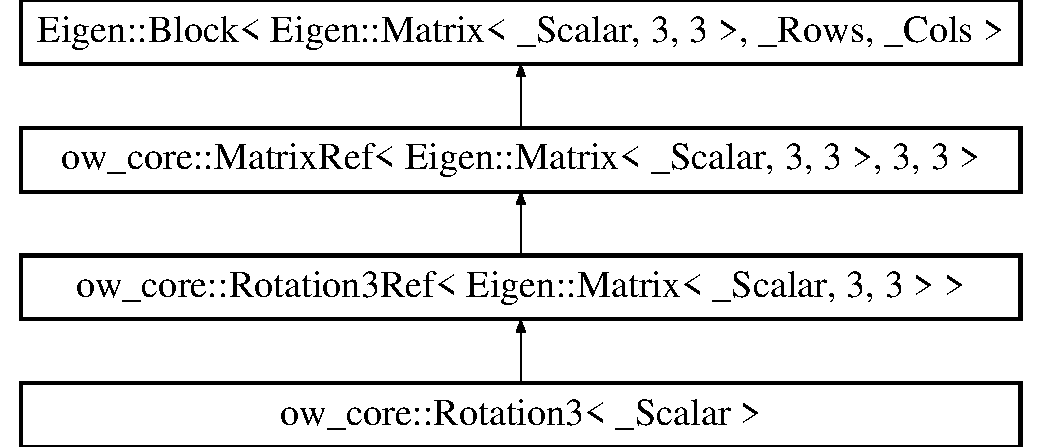
\includegraphics[height=4.000000cm]{db/dd7/classow__core_1_1Rotation3}
\end{center}
\end{figure}
\subsection*{Public Types}
\begin{DoxyCompactItemize}
\item 
typedef \+\_\+\+Scalar {\bfseries Scalar}\hypertarget{classow__core_1_1Rotation3_a470ab3889d669c7c775de59719a05cd5}{}\label{classow__core_1_1Rotation3_a470ab3889d669c7c775de59719a05cd5}

\item 
typedef Eigen\+::\+Matrix$<$ \+\_\+\+Scalar, 3, 3 $>$ {\bfseries Derived}\hypertarget{classow__core_1_1Rotation3_aaa3e83f38709cf7ea047d0a21423b3ef}{}\label{classow__core_1_1Rotation3_aaa3e83f38709cf7ea047d0a21423b3ef}

\item 
typedef \hyperlink{classow__core_1_1Rotation3Ref}{Rotation3\+Ref}$<$ Derived $>$ {\bfseries Base}\hypertarget{classow__core_1_1Rotation3_ae25fa89b75676d23b296fcae485f7b71}{}\label{classow__core_1_1Rotation3_ae25fa89b75676d23b296fcae485f7b71}

\end{DoxyCompactItemize}
\subsection*{Public Member Functions}
\begin{DoxyCompactItemize}
\item 
\hyperlink{classow__core_1_1Rotation3_abd12cb236cf8ff6e5337228633d4815b}{Rotation3} ()\hypertarget{classow__core_1_1Rotation3_abd12cb236cf8ff6e5337228633d4815b}{}\label{classow__core_1_1Rotation3_abd12cb236cf8ff6e5337228633d4815b}

\begin{DoxyCompactList}\small\item\em Default Constructor. \end{DoxyCompactList}\item 
{\footnotesize template$<$typename Other\+Derived $>$ }\\\hyperlink{classow__core_1_1Rotation3_af8f7c2fd09be7d4e7be68c6786114fab}{Rotation3} (const Eigen\+::\+Eigen\+Base$<$ Other\+Derived $>$ \&other)
\begin{DoxyCompactList}\small\item\em Copy constructor. \end{DoxyCompactList}\item 
{\footnotesize template$<$typename Other\+Derived $>$ }\\\hyperlink{classow__core_1_1Rotation3_a34cd49f675144ebc5c6cd50adbd18319}{Rotation3} (const Eigen\+::\+Rotation\+Base$<$ Other\+Derived, 3 $>$ \&other)
\begin{DoxyCompactList}\small\item\em Copy constructor. \end{DoxyCompactList}\end{DoxyCompactItemize}
\subsection*{Protected Attributes}
\begin{DoxyCompactItemize}
\item 
Derived {\bfseries data\+\_\+}\hypertarget{classow__core_1_1Rotation3_a815b7076eb7e0ed4f927cc1668393b7b}{}\label{classow__core_1_1Rotation3_a815b7076eb7e0ed4f927cc1668393b7b}

\end{DoxyCompactItemize}


\subsection{Detailed Description}
\subsubsection*{template$<$typename \+\_\+\+Scalar$>$\\*
class ow\+\_\+core\+::\+Rotation3$<$ \+\_\+\+Scalar $>$}

The \hyperlink{classow__core_1_1Rotation3}{Rotation3} class. 

The \hyperlink{classow__core_1_1Rotation3}{Rotation3} is of type Eigen\+::\+Matrix3 and is represented by the math symbol $\mathbf{R}$. 

\subsection{Constructor \& Destructor Documentation}
\index{ow\+\_\+core\+::\+Rotation3@{ow\+\_\+core\+::\+Rotation3}!Rotation3@{Rotation3}}
\index{Rotation3@{Rotation3}!ow\+\_\+core\+::\+Rotation3@{ow\+\_\+core\+::\+Rotation3}}
\subsubsection[{\texorpdfstring{Rotation3(const Eigen\+::\+Eigen\+Base$<$ Other\+Derived $>$ \&other)}{Rotation3(const Eigen::EigenBase< OtherDerived > &other)}}]{\setlength{\rightskip}{0pt plus 5cm}template$<$typename \+\_\+\+Scalar $>$ template$<$typename Other\+Derived $>$ {\bf ow\+\_\+core\+::\+Rotation3}$<$ \+\_\+\+Scalar $>$\+::{\bf Rotation3} (
\begin{DoxyParamCaption}
\item[{const Eigen\+::\+Eigen\+Base$<$ Other\+Derived $>$ \&}]{other}
\end{DoxyParamCaption}
)\hspace{0.3cm}{\ttfamily [inline]}}\hypertarget{classow__core_1_1Rotation3_af8f7c2fd09be7d4e7be68c6786114fab}{}\label{classow__core_1_1Rotation3_af8f7c2fd09be7d4e7be68c6786114fab}


Copy constructor. 

This copy constructor not only works with Eigen matrices but also with their expressions. \index{ow\+\_\+core\+::\+Rotation3@{ow\+\_\+core\+::\+Rotation3}!Rotation3@{Rotation3}}
\index{Rotation3@{Rotation3}!ow\+\_\+core\+::\+Rotation3@{ow\+\_\+core\+::\+Rotation3}}
\subsubsection[{\texorpdfstring{Rotation3(const Eigen\+::\+Rotation\+Base$<$ Other\+Derived, 3 $>$ \&other)}{Rotation3(const Eigen::RotationBase< OtherDerived, 3 > &other)}}]{\setlength{\rightskip}{0pt plus 5cm}template$<$typename \+\_\+\+Scalar $>$ template$<$typename Other\+Derived $>$ {\bf ow\+\_\+core\+::\+Rotation3}$<$ \+\_\+\+Scalar $>$\+::{\bf Rotation3} (
\begin{DoxyParamCaption}
\item[{const Eigen\+::\+Rotation\+Base$<$ Other\+Derived, 3 $>$ \&}]{other}
\end{DoxyParamCaption}
)\hspace{0.3cm}{\ttfamily [inline]}}\hypertarget{classow__core_1_1Rotation3_a34cd49f675144ebc5c6cd50adbd18319}{}\label{classow__core_1_1Rotation3_a34cd49f675144ebc5c6cd50adbd18319}


Copy constructor. 

This copy constructor works with Eigen Rotation representations. 

The documentation for this class was generated from the following file\+:\begin{DoxyCompactItemize}
\item 
/home/dean/ros/workspaces/ow\+\_\+test\+\_\+ws/src/ow\+\_\+core/include/ow\+\_\+core/\hyperlink{rotation3_8h}{rotation3.\+h}\end{DoxyCompactItemize}

\hypertarget{classow__core_1_1Rotation3Ref}{}\section{ow\+\_\+core\+:\+:Rotation3\+Ref$<$ \+\_\+\+Derived $>$ Class Template Reference}
\label{classow__core_1_1Rotation3Ref}\index{ow\+\_\+core\+::\+Rotation3\+Ref$<$ \+\_\+\+Derived $>$@{ow\+\_\+core\+::\+Rotation3\+Ref$<$ \+\_\+\+Derived $>$}}


The \hyperlink{classow__core_1_1Rotation3Ref}{Rotation3\+Ref} class.  




{\ttfamily \#include $<$rotation3\+\_\+ref.\+h$>$}

Inheritance diagram for ow\+\_\+core\+:\+:Rotation3\+Ref$<$ \+\_\+\+Derived $>$\+:\begin{figure}[H]
\begin{center}
\leavevmode
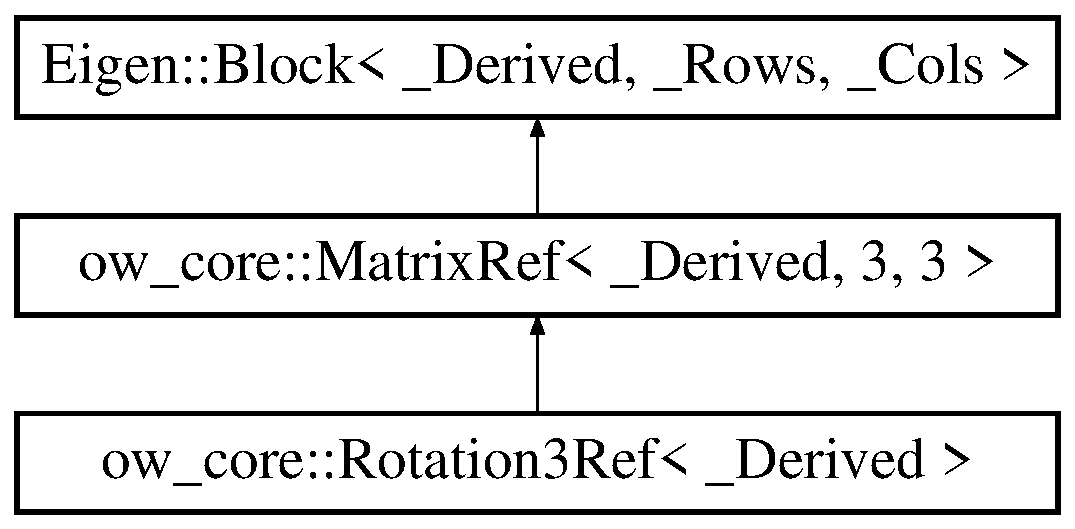
\includegraphics[height=3.000000cm]{dd/d45/classow__core_1_1Rotation3Ref}
\end{center}
\end{figure}
\subsection*{Public Types}
\begin{DoxyCompactItemize}
\item 
typedef \+\_\+\+Derived {\bfseries Derived}\hypertarget{classow__core_1_1Rotation3Ref_a1997d14d4c8143247e57d9543375f613}{}\label{classow__core_1_1Rotation3Ref_a1997d14d4c8143247e57d9543375f613}

\item 
typedef \hyperlink{classow__core_1_1MatrixRef}{Matrix\+Ref}$<$ Derived, 3, 3 $>$ {\bfseries Base}\hypertarget{classow__core_1_1Rotation3Ref_a607f0e4b50d0a3b33152979f6b0fc6f9}{}\label{classow__core_1_1Rotation3Ref_a607f0e4b50d0a3b33152979f6b0fc6f9}

\end{DoxyCompactItemize}
\subsection*{Public Member Functions}
\begin{DoxyCompactItemize}
\item 
\hyperlink{classow__core_1_1Rotation3Ref_a8835f31c0085b6e29af2df3358121b3a}{Rotation3\+Ref} (Derived \&ref, int start\+Row=0, int start\+Col=0)
\begin{DoxyCompactList}\small\item\em Default Constructor. \end{DoxyCompactList}\item 
{\footnotesize template$<$typename Other\+Derived $>$ }\\\hyperlink{classow__core_1_1Rotation3Ref}{Rotation3\+Ref} \& \hyperlink{classow__core_1_1Rotation3Ref_a9b31c385b6c5225f747ea08945642cb8}{operator=} (const Eigen\+::\+Rotation\+Base$<$ Other\+Derived, 3 $>$ \&r)\hypertarget{classow__core_1_1Rotation3Ref_a9b31c385b6c5225f747ea08945642cb8}{}\label{classow__core_1_1Rotation3Ref_a9b31c385b6c5225f747ea08945642cb8}

\begin{DoxyCompactList}\small\item\em Assignment of Eigen\+::\+Rotation\+Base. \end{DoxyCompactList}\item 
void \hyperlink{classow__core_1_1Rotation3Ref_a0b58716ea88baa8d13515bbe5ffe76f2}{operator=} (const tf\+::\+Quaternion \&q)\hypertarget{classow__core_1_1Rotation3Ref_a0b58716ea88baa8d13515bbe5ffe76f2}{}\label{classow__core_1_1Rotation3Ref_a0b58716ea88baa8d13515bbe5ffe76f2}

\begin{DoxyCompactList}\small\item\em Assignment of tf\+::\+Quaternion. \end{DoxyCompactList}\item 
void \hyperlink{classow__core_1_1Rotation3Ref_a4823dd9bcb419d9f92b1fce8f88d495a}{operator=} (const geometry\+\_\+msgs\+::\+Quaternion \&q)\hypertarget{classow__core_1_1Rotation3Ref_a4823dd9bcb419d9f92b1fce8f88d495a}{}\label{classow__core_1_1Rotation3Ref_a4823dd9bcb419d9f92b1fce8f88d495a}

\begin{DoxyCompactList}\small\item\em Assignment of geometry\+\_\+msgs\+::\+Quaternion. \end{DoxyCompactList}\item 
void \hyperlink{classow__core_1_1Rotation3Ref_a8f91b728de1db5da5775121c358e0521}{operator=} (const tf\+::\+Matrix3x3 \&R)\hypertarget{classow__core_1_1Rotation3Ref_a8f91b728de1db5da5775121c358e0521}{}\label{classow__core_1_1Rotation3Ref_a8f91b728de1db5da5775121c358e0521}

\begin{DoxyCompactList}\small\item\em Assignment of tf\+::\+Matrix3x3. \end{DoxyCompactList}\item 
\hyperlink{classow__core_1_1Rotation3Ref_ae7464db927a40cd9fbb5109169b7bb22}{operator tf\+::\+Quaternion} () const \hypertarget{classow__core_1_1Rotation3Ref_ae7464db927a40cd9fbb5109169b7bb22}{}\label{classow__core_1_1Rotation3Ref_ae7464db927a40cd9fbb5109169b7bb22}

\begin{DoxyCompactList}\small\item\em Conversion to tf\+::\+Quaternion. \end{DoxyCompactList}\item 
\hyperlink{classow__core_1_1Rotation3Ref_ae438d192b6b3d0d17331f26275370720}{operator geometry\+\_\+msgs\+::\+Quaternion} () const \hypertarget{classow__core_1_1Rotation3Ref_ae438d192b6b3d0d17331f26275370720}{}\label{classow__core_1_1Rotation3Ref_ae438d192b6b3d0d17331f26275370720}

\begin{DoxyCompactList}\small\item\em Conversion to geometry\+\_\+msgs\+::\+Quaternion. \end{DoxyCompactList}\item 
\hyperlink{classow__core_1_1Rotation3Ref_afc7e55ed5108a0ca56b6ef524be4962a}{operator tf\+::\+Matrix3x3} () const \hypertarget{classow__core_1_1Rotation3Ref_afc7e55ed5108a0ca56b6ef524be4962a}{}\label{classow__core_1_1Rotation3Ref_afc7e55ed5108a0ca56b6ef524be4962a}

\begin{DoxyCompactList}\small\item\em Conversion to tf\+::\+Matrix3x3. \end{DoxyCompactList}\item 
tf\+::\+Quaternion \hyperlink{classow__core_1_1Rotation3Ref_ad6db993cebda82f1b8f6d8ef78a498bf}{to\+Quaternion\+TF} ()\hypertarget{classow__core_1_1Rotation3Ref_ad6db993cebda82f1b8f6d8ef78a498bf}{}\label{classow__core_1_1Rotation3Ref_ad6db993cebda82f1b8f6d8ef78a498bf}

\begin{DoxyCompactList}\small\item\em Conversion to tf\+::\+Quaternion. \end{DoxyCompactList}\item 
geometry\+\_\+msgs\+::\+Quaternion \hyperlink{classow__core_1_1Rotation3Ref_a05ed8df1030e9d3370b6b25a03d5e140}{to\+Quaternion\+Msg} ()\hypertarget{classow__core_1_1Rotation3Ref_a05ed8df1030e9d3370b6b25a03d5e140}{}\label{classow__core_1_1Rotation3Ref_a05ed8df1030e9d3370b6b25a03d5e140}

\begin{DoxyCompactList}\small\item\em Conversion to geometry\+\_\+msgs\+::\+Quaternion. \end{DoxyCompactList}\item 
tf\+::\+Matrix3x3 \hyperlink{classow__core_1_1Rotation3Ref_ae0f85728772cde3bd954e7b86a4a4f22}{to\+Matrix\+TF} ()\hypertarget{classow__core_1_1Rotation3Ref_ae0f85728772cde3bd954e7b86a4a4f22}{}\label{classow__core_1_1Rotation3Ref_ae0f85728772cde3bd954e7b86a4a4f22}

\begin{DoxyCompactList}\small\item\em Conversion to tf\+::\+Matrix3x3. \end{DoxyCompactList}\end{DoxyCompactItemize}


\subsection{Detailed Description}
\subsubsection*{template$<$typename \+\_\+\+Derived$>$\\*
class ow\+\_\+core\+::\+Rotation3\+Ref$<$ \+\_\+\+Derived $>$}

The \hyperlink{classow__core_1_1Rotation3Ref}{Rotation3\+Ref} class. 

The \hyperlink{classow__core_1_1Rotation3}{Rotation3} is of type Eigen\+::\+Matrix3 and is represented by the math symbol $\mathbf{R}$.

References the data of another Eigen type class via Eigen\+::\+Block. 

\subsection{Constructor \& Destructor Documentation}
\index{ow\+\_\+core\+::\+Rotation3\+Ref@{ow\+\_\+core\+::\+Rotation3\+Ref}!Rotation3\+Ref@{Rotation3\+Ref}}
\index{Rotation3\+Ref@{Rotation3\+Ref}!ow\+\_\+core\+::\+Rotation3\+Ref@{ow\+\_\+core\+::\+Rotation3\+Ref}}
\subsubsection[{\texorpdfstring{Rotation3\+Ref(\+Derived \&ref, int start\+Row=0, int start\+Col=0)}{Rotation3Ref(Derived &ref, int startRow=0, int startCol=0)}}]{\setlength{\rightskip}{0pt plus 5cm}template$<$typename \+\_\+\+Derived$>$ {\bf ow\+\_\+core\+::\+Rotation3\+Ref}$<$ \+\_\+\+Derived $>$\+::{\bf Rotation3\+Ref} (
\begin{DoxyParamCaption}
\item[{Derived \&}]{ref, }
\item[{int}]{start\+Row = {\ttfamily 0}, }
\item[{int}]{start\+Col = {\ttfamily 0}}
\end{DoxyParamCaption}
)\hspace{0.3cm}{\ttfamily [inline]}, {\ttfamily [explicit]}}\hypertarget{classow__core_1_1Rotation3Ref_a8835f31c0085b6e29af2df3358121b3a}{}\label{classow__core_1_1Rotation3Ref_a8835f31c0085b6e29af2df3358121b3a}


Default Constructor. 


\begin{DoxyParams}{Parameters}
{\em ref} & the reference to storage Eigen object to access the elements of the \hyperlink{classow__core_1_1LinearPosition}{Linear\+Position} via Eigen\+::\+Block.\\
\hline
{\em start\+Row} & the start index of the row for Eigen\+::\+Block.\\
\hline
{\em start\+Col} & the start index of the column for Eigen\+::\+Block. \\
\hline
\end{DoxyParams}


The documentation for this class was generated from the following file\+:\begin{DoxyCompactItemize}
\item 
/home/dean/ros/workspaces/ow\+\_\+test\+\_\+ws/src/ow\+\_\+core/include/ow\+\_\+core/\hyperlink{rotation3__ref_8h}{rotation3\+\_\+ref.\+h}\end{DoxyCompactItemize}

\hypertarget{structEigen_1_1internal_1_1traits_3_01QuaternionRef_3_01__Derived_01_4_01_4}{}\section{Eigen\+:\+:internal\+:\+:traits$<$ Quaternion\+Ref$<$ \+\_\+\+Derived $>$ $>$ Struct Template Reference}
\label{structEigen_1_1internal_1_1traits_3_01QuaternionRef_3_01__Derived_01_4_01_4}\index{Eigen\+::internal\+::traits$<$ Quaternion\+Ref$<$ \+\_\+\+Derived $>$ $>$@{Eigen\+::internal\+::traits$<$ Quaternion\+Ref$<$ \+\_\+\+Derived $>$ $>$}}


The traits class for \hyperlink{classEigen_1_1QuaternionRef}{Quaternion\+Ref}.  




{\ttfamily \#include $<$quaternion\+\_\+ref.\+h$>$}

\subsection*{Public Types}
\begin{DoxyCompactItemize}
\item 
enum \{ {\bfseries Alignment} = internal\+:\+:traits$<$Coefficients$>$\+:\+:Alignment, 
{\bfseries Flags} = Lvalue\+Bit
 \}\hypertarget{structEigen_1_1internal_1_1traits_3_01QuaternionRef_3_01__Derived_01_4_01_4_acd608453e0cd4940f6f49964daa8e84e}{}\label{structEigen_1_1internal_1_1traits_3_01QuaternionRef_3_01__Derived_01_4_01_4_acd608453e0cd4940f6f49964daa8e84e}

\item 
typedef \hyperlink{classEigen_1_1QuaternionRef}{Quaternion\+Ref}$<$ \+\_\+\+Derived $>$ {\bfseries Plain\+Object}\hypertarget{structEigen_1_1internal_1_1traits_3_01QuaternionRef_3_01__Derived_01_4_01_4_afb4148e5066544aadd54ebee6c0a6f5d}{}\label{structEigen_1_1internal_1_1traits_3_01QuaternionRef_3_01__Derived_01_4_01_4_afb4148e5066544aadd54ebee6c0a6f5d}

\item 
typedef \+\_\+\+Derived\+::\+Scalar {\bfseries Scalar}\hypertarget{structEigen_1_1internal_1_1traits_3_01QuaternionRef_3_01__Derived_01_4_01_4_a24e9f1afdf166a5dd1f61db147199699}{}\label{structEigen_1_1internal_1_1traits_3_01QuaternionRef_3_01__Derived_01_4_01_4_a24e9f1afdf166a5dd1f61db147199699}

\item 
typedef Eigen\+::\+Block$<$ \+\_\+\+Derived, 4, 1 $>$ {\bfseries Coefficients}\hypertarget{structEigen_1_1internal_1_1traits_3_01QuaternionRef_3_01__Derived_01_4_01_4_a2eb1c923a6451a17be2966e89306eae3}{}\label{structEigen_1_1internal_1_1traits_3_01QuaternionRef_3_01__Derived_01_4_01_4_a2eb1c923a6451a17be2966e89306eae3}

\end{DoxyCompactItemize}


\subsection{Detailed Description}
\subsubsection*{template$<$typename \+\_\+\+Derived$>$\\*
struct Eigen\+::internal\+::traits$<$ Quaternion\+Ref$<$ \+\_\+\+Derived $>$ $>$}

The traits class for \hyperlink{classEigen_1_1QuaternionRef}{Quaternion\+Ref}. 

This class contains the typedefs and enums for the \hyperlink{classEigen_1_1QuaternionRef}{Eigen\+::\+Quaternion\+Ref} class.

These typedefs and enums are used to define and describe the properties (traits) of the new class. The templates of the Eigen library heavily depend on the traits to properly handle the different type classes.

N\+O\+TE\+: Since the Eigen library uses the \char`\"{}\+Curiously Recurring Template Pattern\char`\"{} (read \href{https://eigen.tuxfamily.org/dox/TopicInsideEigenExample.html}{\tt https\+://eigen.\+tuxfamily.\+org/dox/\+Topic\+Inside\+Eigen\+Example.\+html}) the new Eigen type class has to be defined in the Eigen namespace.

\begin{DoxyRefDesc}{Todo}
\item[\hyperlink{todo__todo000005}{Todo}]Maybe the Eigen\+::\+Block args should be parameters. One might want to select a column vector. \end{DoxyRefDesc}


The documentation for this struct was generated from the following file\+:\begin{DoxyCompactItemize}
\item 
/home/dean/ros/workspaces/ow\+\_\+test\+\_\+ws/src/ow\+\_\+core/include/ow\+\_\+core/\+Eigen/\hyperlink{Eigen_2quaternion__ref_8h}{quaternion\+\_\+ref.\+h}\end{DoxyCompactItemize}

\hypertarget{classow__core_1_1Vector3}{}\section{ow\+\_\+core\+:\+:Vector3$<$ \+\_\+\+Scalar $>$ Class Template Reference}
\label{classow__core_1_1Vector3}\index{ow\+\_\+core\+::\+Vector3$<$ \+\_\+\+Scalar $>$@{ow\+\_\+core\+::\+Vector3$<$ \+\_\+\+Scalar $>$}}


The \hyperlink{classow__core_1_1Vector3}{Vector3} class.  




{\ttfamily \#include $<$vector3.\+h$>$}

Inheritance diagram for ow\+\_\+core\+:\+:Vector3$<$ \+\_\+\+Scalar $>$\+:\begin{figure}[H]
\begin{center}
\leavevmode
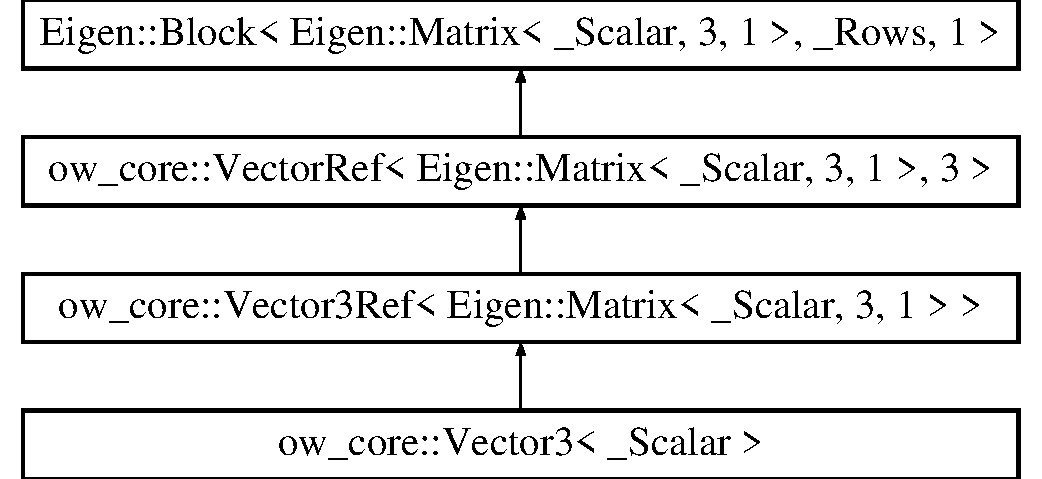
\includegraphics[height=4.000000cm]{df/dc3/classow__core_1_1Vector3}
\end{center}
\end{figure}
\subsection*{Public Types}
\begin{DoxyCompactItemize}
\item 
typedef \+\_\+\+Scalar {\bfseries Scalar}\hypertarget{classow__core_1_1Vector3_a13a53dc729069a5c30a2c188bbbffbe4}{}\label{classow__core_1_1Vector3_a13a53dc729069a5c30a2c188bbbffbe4}

\item 
typedef Eigen\+::\+Matrix$<$ \+\_\+\+Scalar, 3, 1 $>$ {\bfseries Derived}\hypertarget{classow__core_1_1Vector3_ae043e39ab4ca8568831379647aeaa20b}{}\label{classow__core_1_1Vector3_ae043e39ab4ca8568831379647aeaa20b}

\item 
typedef \hyperlink{classow__core_1_1Vector3Ref}{Vector3\+Ref}$<$ Derived $>$ {\bfseries Base}\hypertarget{classow__core_1_1Vector3_a2eecdfd19c036b760f0a727fe5c60ba1}{}\label{classow__core_1_1Vector3_a2eecdfd19c036b760f0a727fe5c60ba1}

\end{DoxyCompactItemize}
\subsection*{Public Member Functions}
\begin{DoxyCompactItemize}
\item 
\hyperlink{classow__core_1_1Vector3_ae2c63c465a844cf260607beed2851620}{Vector3} ()\hypertarget{classow__core_1_1Vector3_ae2c63c465a844cf260607beed2851620}{}\label{classow__core_1_1Vector3_ae2c63c465a844cf260607beed2851620}

\begin{DoxyCompactList}\small\item\em Default Constructor. \end{DoxyCompactList}\item 
\hyperlink{classow__core_1_1Vector3_ab4e68ba3b96f153fe14408823a600332}{Vector3} (const Scalar \&x, const Scalar \&y, const Scalar \&z)\hypertarget{classow__core_1_1Vector3_ab4e68ba3b96f153fe14408823a600332}{}\label{classow__core_1_1Vector3_ab4e68ba3b96f153fe14408823a600332}

\begin{DoxyCompactList}\small\item\em Assignment from Scalar values. \end{DoxyCompactList}\item 
{\footnotesize template$<$typename Other\+Derived $>$ }\\\hyperlink{classow__core_1_1Vector3_ac80729ad78e79dff06e14d95b372945a}{Vector3} (const Eigen\+::\+Eigen\+Base$<$ Other\+Derived $>$ \&other)
\begin{DoxyCompactList}\small\item\em Copy constructor. \end{DoxyCompactList}\end{DoxyCompactItemize}
\subsection*{Protected Attributes}
\begin{DoxyCompactItemize}
\item 
Derived {\bfseries data\+\_\+}\hypertarget{classow__core_1_1Vector3_a1f3977149a1a461518a47bc68b831c6e}{}\label{classow__core_1_1Vector3_a1f3977149a1a461518a47bc68b831c6e}

\end{DoxyCompactItemize}


\subsection{Detailed Description}
\subsubsection*{template$<$typename \+\_\+\+Scalar$>$\\*
class ow\+\_\+core\+::\+Vector3$<$ \+\_\+\+Scalar $>$}

The \hyperlink{classow__core_1_1Vector3}{Vector3} class. 

The \hyperlink{classow__core_1_1Vector3}{Vector3} is of type Eigen\+::\+Vector3 and is represented by the math symbol ${\mathbf{v}}$. 

\subsection{Constructor \& Destructor Documentation}
\index{ow\+\_\+core\+::\+Vector3@{ow\+\_\+core\+::\+Vector3}!Vector3@{Vector3}}
\index{Vector3@{Vector3}!ow\+\_\+core\+::\+Vector3@{ow\+\_\+core\+::\+Vector3}}
\subsubsection[{\texorpdfstring{Vector3(const Eigen\+::\+Eigen\+Base$<$ Other\+Derived $>$ \&other)}{Vector3(const Eigen::EigenBase< OtherDerived > &other)}}]{\setlength{\rightskip}{0pt plus 5cm}template$<$typename \+\_\+\+Scalar $>$ template$<$typename Other\+Derived $>$ {\bf ow\+\_\+core\+::\+Vector3}$<$ \+\_\+\+Scalar $>$\+::{\bf Vector3} (
\begin{DoxyParamCaption}
\item[{const Eigen\+::\+Eigen\+Base$<$ Other\+Derived $>$ \&}]{other}
\end{DoxyParamCaption}
)\hspace{0.3cm}{\ttfamily [inline]}}\hypertarget{classow__core_1_1Vector3_ac80729ad78e79dff06e14d95b372945a}{}\label{classow__core_1_1Vector3_ac80729ad78e79dff06e14d95b372945a}


Copy constructor. 

This copy constructor not only works with Eigen matrices but also with their expressions. 

The documentation for this class was generated from the following file\+:\begin{DoxyCompactItemize}
\item 
/home/dean/ros/workspaces/ow\+\_\+test\+\_\+ws/src/ow\+\_\+core/include/ow\+\_\+core/\hyperlink{vector3_8h}{vector3.\+h}\end{DoxyCompactItemize}

\hypertarget{classow__core_1_1Vector3Ref}{}\section{ow\+\_\+core\+:\+:Vector3\+Ref$<$ \+\_\+\+Derived $>$ Class Template Reference}
\label{classow__core_1_1Vector3Ref}\index{ow\+\_\+core\+::\+Vector3\+Ref$<$ \+\_\+\+Derived $>$@{ow\+\_\+core\+::\+Vector3\+Ref$<$ \+\_\+\+Derived $>$}}


The \hyperlink{classow__core_1_1Vector3Ref}{Vector3\+Ref} class.  




{\ttfamily \#include $<$vector3\+\_\+ref.\+h$>$}

Inheritance diagram for ow\+\_\+core\+:\+:Vector3\+Ref$<$ \+\_\+\+Derived $>$\+:\begin{figure}[H]
\begin{center}
\leavevmode
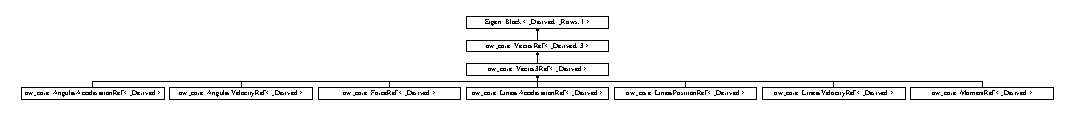
\includegraphics[height=1.114983cm]{d2/d0b/classow__core_1_1Vector3Ref}
\end{center}
\end{figure}
\subsection*{Public Types}
\begin{DoxyCompactItemize}
\item 
typedef \+\_\+\+Derived {\bfseries Derived}\hypertarget{classow__core_1_1Vector3Ref_aa0de46e47cfd8bc910d62ba5b3d5941c}{}\label{classow__core_1_1Vector3Ref_aa0de46e47cfd8bc910d62ba5b3d5941c}

\item 
typedef \hyperlink{classow__core_1_1VectorRef}{Vector\+Ref}$<$ Derived, 3 $>$ {\bfseries Base}\hypertarget{classow__core_1_1Vector3Ref_acda9aca9c1bf20bdd01ac037c1890055}{}\label{classow__core_1_1Vector3Ref_acda9aca9c1bf20bdd01ac037c1890055}

\end{DoxyCompactItemize}
\subsection*{Public Member Functions}
\begin{DoxyCompactItemize}
\item 
\hyperlink{classow__core_1_1Vector3Ref_adc8168bca617c01e8eaeeda9c39db95f}{Vector3\+Ref} (Derived \&ref, int start\+Row=0, int start\+Col=0)
\begin{DoxyCompactList}\small\item\em Default Constructor. \end{DoxyCompactList}\item 
void \hyperlink{classow__core_1_1Vector3Ref_a38395e2f18034252ac105b84c96007d9}{operator=} (const tf\+::\+Vector3 \&x)\hypertarget{classow__core_1_1Vector3Ref_a38395e2f18034252ac105b84c96007d9}{}\label{classow__core_1_1Vector3Ref_a38395e2f18034252ac105b84c96007d9}

\begin{DoxyCompactList}\small\item\em Assignment of tf\+::\+Vector3. \end{DoxyCompactList}\item 
void \hyperlink{classow__core_1_1Vector3Ref_a1807832ba87ce4159fdc35898c4ec275}{operator=} (const geometry\+\_\+msgs\+::\+Vector3 \&x)\hypertarget{classow__core_1_1Vector3Ref_a1807832ba87ce4159fdc35898c4ec275}{}\label{classow__core_1_1Vector3Ref_a1807832ba87ce4159fdc35898c4ec275}

\begin{DoxyCompactList}\small\item\em Assignment of geometry\+\_\+msgs\+::\+Vector3. \end{DoxyCompactList}\item 
void \hyperlink{classow__core_1_1Vector3Ref_a405e991adbc0653d414af78e507895d0}{operator=} (const geometry\+\_\+msgs\+::\+Point \&x)\hypertarget{classow__core_1_1Vector3Ref_a405e991adbc0653d414af78e507895d0}{}\label{classow__core_1_1Vector3Ref_a405e991adbc0653d414af78e507895d0}

\begin{DoxyCompactList}\small\item\em Assignment of geometry\+\_\+msgs\+::\+Point. \end{DoxyCompactList}\item 
\hyperlink{classow__core_1_1Vector3Ref_ad68d850a8194ff0ef38dced99c4c04de}{operator tf\+::\+Vector3} () const \hypertarget{classow__core_1_1Vector3Ref_ad68d850a8194ff0ef38dced99c4c04de}{}\label{classow__core_1_1Vector3Ref_ad68d850a8194ff0ef38dced99c4c04de}

\begin{DoxyCompactList}\small\item\em Conversion to tf\+::\+Vector3. \end{DoxyCompactList}\item 
\hyperlink{classow__core_1_1Vector3Ref_a0fa93408729b260afd057080b6acdbeb}{operator geometry\+\_\+msgs\+::\+Point} () const \hypertarget{classow__core_1_1Vector3Ref_a0fa93408729b260afd057080b6acdbeb}{}\label{classow__core_1_1Vector3Ref_a0fa93408729b260afd057080b6acdbeb}

\begin{DoxyCompactList}\small\item\em Conversion to geometry\+\_\+msgs\+::\+Point. \end{DoxyCompactList}\item 
\hyperlink{classow__core_1_1Vector3Ref_a8ada21757d1605bea6abe32b164a8b18}{operator geometry\+\_\+msgs\+::\+Vector3} () const \hypertarget{classow__core_1_1Vector3Ref_a8ada21757d1605bea6abe32b164a8b18}{}\label{classow__core_1_1Vector3Ref_a8ada21757d1605bea6abe32b164a8b18}

\begin{DoxyCompactList}\small\item\em Conversion to geometry\+\_\+msgs\+::\+Point. \end{DoxyCompactList}\item 
tf\+::\+Vector3 \hyperlink{classow__core_1_1Vector3Ref_a19d6773e362b9c1117b43227b82d9d49}{to\+Vector\+TF} () const \hypertarget{classow__core_1_1Vector3Ref_a19d6773e362b9c1117b43227b82d9d49}{}\label{classow__core_1_1Vector3Ref_a19d6773e362b9c1117b43227b82d9d49}

\begin{DoxyCompactList}\small\item\em Conversion to tf\+::\+Vector3. \end{DoxyCompactList}\item 
geometry\+\_\+msgs\+::\+Point \hyperlink{classow__core_1_1Vector3Ref_a6a3676b629ef710c1f626e2c0bb4a683}{to\+Point\+Msg} () const \hypertarget{classow__core_1_1Vector3Ref_a6a3676b629ef710c1f626e2c0bb4a683}{}\label{classow__core_1_1Vector3Ref_a6a3676b629ef710c1f626e2c0bb4a683}

\begin{DoxyCompactList}\small\item\em Conversion to geometry\+\_\+msgs\+::\+Point. \end{DoxyCompactList}\item 
geometry\+\_\+msgs\+::\+Vector3 \hyperlink{classow__core_1_1Vector3Ref_a00dd58af16b78fd7b882d2d253d8e0d4}{to\+Vector3\+Msg} () const \hypertarget{classow__core_1_1Vector3Ref_a00dd58af16b78fd7b882d2d253d8e0d4}{}\label{classow__core_1_1Vector3Ref_a00dd58af16b78fd7b882d2d253d8e0d4}

\begin{DoxyCompactList}\small\item\em Conversion to geometry\+\_\+msgs\+::\+Point. \end{DoxyCompactList}\end{DoxyCompactItemize}


\subsection{Detailed Description}
\subsubsection*{template$<$typename \+\_\+\+Derived$>$\\*
class ow\+\_\+core\+::\+Vector3\+Ref$<$ \+\_\+\+Derived $>$}

The \hyperlink{classow__core_1_1Vector3Ref}{Vector3\+Ref} class. 

The \hyperlink{classow__core_1_1Vector3Ref}{Vector3\+Ref} is of type Eigen\+::\+Vector3 and is represented by the math symbol $\dot{\mathbf{x}}$.

References the data of another Eigen type class via Eigen\+::\+Block. 

\subsection{Constructor \& Destructor Documentation}
\index{ow\+\_\+core\+::\+Vector3\+Ref@{ow\+\_\+core\+::\+Vector3\+Ref}!Vector3\+Ref@{Vector3\+Ref}}
\index{Vector3\+Ref@{Vector3\+Ref}!ow\+\_\+core\+::\+Vector3\+Ref@{ow\+\_\+core\+::\+Vector3\+Ref}}
\subsubsection[{\texorpdfstring{Vector3\+Ref(\+Derived \&ref, int start\+Row=0, int start\+Col=0)}{Vector3Ref(Derived &ref, int startRow=0, int startCol=0)}}]{\setlength{\rightskip}{0pt plus 5cm}template$<$typename \+\_\+\+Derived$>$ {\bf ow\+\_\+core\+::\+Vector3\+Ref}$<$ \+\_\+\+Derived $>$\+::{\bf Vector3\+Ref} (
\begin{DoxyParamCaption}
\item[{Derived \&}]{ref, }
\item[{int}]{start\+Row = {\ttfamily 0}, }
\item[{int}]{start\+Col = {\ttfamily 0}}
\end{DoxyParamCaption}
)\hspace{0.3cm}{\ttfamily [inline]}, {\ttfamily [explicit]}}\hypertarget{classow__core_1_1Vector3Ref_adc8168bca617c01e8eaeeda9c39db95f}{}\label{classow__core_1_1Vector3Ref_adc8168bca617c01e8eaeeda9c39db95f}


Default Constructor. 


\begin{DoxyParams}{Parameters}
{\em ref} & the reference to storage Eigen object to access the elements of the \hyperlink{classow__core_1_1LinearPosition}{Linear\+Position} via Eigen\+::\+Block.\\
\hline
{\em start\+Row} & the start index of the row for Eigen\+::\+Block.\\
\hline
{\em start\+Col} & the start index of the column for Eigen\+::\+Block. \\
\hline
\end{DoxyParams}


The documentation for this class was generated from the following file\+:\begin{DoxyCompactItemize}
\item 
/home/dean/ros/workspaces/ow\+\_\+test\+\_\+ws/src/ow\+\_\+core/include/ow\+\_\+core/\hyperlink{vector3__ref_8h}{vector3\+\_\+ref.\+h}\end{DoxyCompactItemize}

\hypertarget{classow__core_1_1VectorDof}{}\section{ow\+\_\+core\+:\+:Vector\+Dof$<$ \+\_\+\+Scalar, \+\_\+\+Rows $>$ Class Template Reference}
\label{classow__core_1_1VectorDof}\index{ow\+\_\+core\+::\+Vector\+Dof$<$ \+\_\+\+Scalar, \+\_\+\+Rows $>$@{ow\+\_\+core\+::\+Vector\+Dof$<$ \+\_\+\+Scalar, \+\_\+\+Rows $>$}}


The \hyperlink{classow__core_1_1VectorDof}{Vector\+Dof} class.  




{\ttfamily \#include $<$vector\+\_\+dof.\+h$>$}

Inheritance diagram for ow\+\_\+core\+:\+:Vector\+Dof$<$ \+\_\+\+Scalar, \+\_\+\+Rows $>$\+:\begin{figure}[H]
\begin{center}
\leavevmode
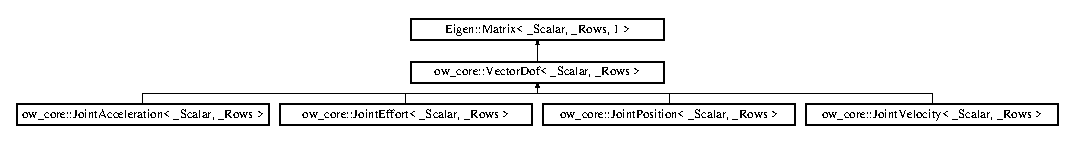
\includegraphics[height=1.458333cm]{d9/d10/classow__core_1_1VectorDof}
\end{center}
\end{figure}
\subsection*{Public Types}
\begin{DoxyCompactItemize}
\item 
enum \{ {\bfseries Rows} = \+\_\+\+Rows
 \}\hypertarget{classow__core_1_1VectorDof_a7c5a7ddd6224d55ca6c638399a160a17}{}\label{classow__core_1_1VectorDof_a7c5a7ddd6224d55ca6c638399a160a17}

\item 
typedef \+\_\+\+Scalar {\bfseries Scalar}\hypertarget{classow__core_1_1VectorDof_acf92659e64b4ee228fbf3ae573680655}{}\label{classow__core_1_1VectorDof_acf92659e64b4ee228fbf3ae573680655}

\item 
typedef Eigen\+::\+Matrix$<$ Scalar, Rows, 1 $>$ {\bfseries Base}\hypertarget{classow__core_1_1VectorDof_a797da821d2fab9e447eab836718293ef}{}\label{classow__core_1_1VectorDof_a797da821d2fab9e447eab836718293ef}

\end{DoxyCompactItemize}
\subsection*{Public Member Functions}
\begin{DoxyCompactItemize}
\item 
\hyperlink{classow__core_1_1VectorDof_a488ac8cc1bfe0683f6d348eca855735d}{Vector\+Dof} ()\hypertarget{classow__core_1_1VectorDof_a488ac8cc1bfe0683f6d348eca855735d}{}\label{classow__core_1_1VectorDof_a488ac8cc1bfe0683f6d348eca855735d}

\begin{DoxyCompactList}\small\item\em Default Constructor. \end{DoxyCompactList}\item 
{\footnotesize template$<$typename Other\+Derived $>$ }\\\hyperlink{classow__core_1_1VectorDof_a52fb1369e02f8b20b6510f6bdef6ca12}{Vector\+Dof} (const Eigen\+::\+Eigen\+Base$<$ Other\+Derived $>$ \&other)
\begin{DoxyCompactList}\small\item\em Copy constructor. \end{DoxyCompactList}\item 
\hyperlink{classow__core_1_1VectorDof}{Vector\+Dof} \& {\bfseries set\+Constant} (const Scalar \&value)\hypertarget{classow__core_1_1VectorDof_acd67ace1b66bed1d51c0762dc62ba9a7}{}\label{classow__core_1_1VectorDof_acd67ace1b66bed1d51c0762dc62ba9a7}

\item 
\hyperlink{classow__core_1_1VectorDof}{Vector\+Dof} \& {\bfseries set\+Lin\+Spaced} (const Scalar \&low, const Scalar \&high)\hypertarget{classow__core_1_1VectorDof_a85cb5a00ad47f5d9046780b4e63271ac}{}\label{classow__core_1_1VectorDof_a85cb5a00ad47f5d9046780b4e63271ac}

\item 
\hyperlink{classow__core_1_1VectorDof}{Vector\+Dof} \& {\bfseries set\+Zero} ()\hypertarget{classow__core_1_1VectorDof_adb9403a5726589146cec53b98ce27a50}{}\label{classow__core_1_1VectorDof_adb9403a5726589146cec53b98ce27a50}

\item 
\hyperlink{classow__core_1_1VectorDof}{Vector\+Dof} \& {\bfseries set\+Ones} ()\hypertarget{classow__core_1_1VectorDof_a079291e0d1a46a048066ca31a4c52d7b}{}\label{classow__core_1_1VectorDof_a079291e0d1a46a048066ca31a4c52d7b}

\item 
\hyperlink{classow__core_1_1VectorDof}{Vector\+Dof} \& {\bfseries set\+Random} ()\hypertarget{classow__core_1_1VectorDof_a788e7aaeffb52db4a9fcb14ad84fc6eb}{}\label{classow__core_1_1VectorDof_a788e7aaeffb52db4a9fcb14ad84fc6eb}

\item 
std\+::string \hyperlink{classow__core_1_1VectorDof_aca0f060adbac385e9ef350947248041c}{to\+String} () const \hypertarget{classow__core_1_1VectorDof_aca0f060adbac385e9ef350947248041c}{}\label{classow__core_1_1VectorDof_aca0f060adbac385e9ef350947248041c}

\begin{DoxyCompactList}\small\item\em Conversion to std\+::string. \end{DoxyCompactList}\end{DoxyCompactItemize}
\subsection*{Static Public Member Functions}
\begin{DoxyCompactItemize}
\item 
static Base\+::\+Constant\+Return\+Type \hyperlink{classow__core_1_1VectorDof_a9e6be2c39b494db7b7d4ed62bdf6cbe3}{Zero} ()
\begin{DoxyCompactList}\small\item\em Returns an expression where all coefficients equal zero. \end{DoxyCompactList}\item 
static Base\+::\+Constant\+Return\+Type \hyperlink{classow__core_1_1VectorDof_abbb267905416971fa0edd4224f3cf428}{Ones} ()\hypertarget{classow__core_1_1VectorDof_abbb267905416971fa0edd4224f3cf428}{}\label{classow__core_1_1VectorDof_abbb267905416971fa0edd4224f3cf428}

\begin{DoxyCompactList}\small\item\em Returns an expression where all coefficients equal one. \end{DoxyCompactList}\item 
static Base\+::\+Constant\+Return\+Type \hyperlink{classow__core_1_1VectorDof_afa6d09d81da823ac3ea27b431a3e3a42}{Constant} (const Scalar \&value)\hypertarget{classow__core_1_1VectorDof_afa6d09d81da823ac3ea27b431a3e3a42}{}\label{classow__core_1_1VectorDof_afa6d09d81da823ac3ea27b431a3e3a42}

\begin{DoxyCompactList}\small\item\em Returns an expression where all coefficients equal the given value. \end{DoxyCompactList}\item 
static const Base\+::\+Random\+Return\+Type \hyperlink{classow__core_1_1VectorDof_af30f677b67b4b2a3d50dd58d17f13dd4}{Random} ()\hypertarget{classow__core_1_1VectorDof_af30f677b67b4b2a3d50dd58d17f13dd4}{}\label{classow__core_1_1VectorDof_af30f677b67b4b2a3d50dd58d17f13dd4}

\begin{DoxyCompactList}\small\item\em Returns an expression where all coefficients are random. \end{DoxyCompactList}\item 
static const Base\+::\+Basis\+Return\+Type \hyperlink{classow__core_1_1VectorDof_ac2f8c5af2c4ddab88a0c931b1b8f6b43}{Unit} (typename Base\+::\+Index i)\hypertarget{classow__core_1_1VectorDof_ac2f8c5af2c4ddab88a0c931b1b8f6b43}{}\label{classow__core_1_1VectorDof_ac2f8c5af2c4ddab88a0c931b1b8f6b43}

\begin{DoxyCompactList}\small\item\em Returns an expression where all coefficients represent the i-\/th basis vector. \end{DoxyCompactList}\end{DoxyCompactItemize}


\subsection{Detailed Description}
\subsubsection*{template$<$typename \+\_\+\+Scalar, int \+\_\+\+Rows$>$\\*
class ow\+\_\+core\+::\+Vector\+Dof$<$ \+\_\+\+Scalar, \+\_\+\+Rows $>$}

The \hyperlink{classow__core_1_1VectorDof}{Vector\+Dof} class. 

The \hyperlink{classow__core_1_1VectorDof}{Vector\+Dof} is of type Eigen\+::\+Matrix. 

\subsection{Constructor \& Destructor Documentation}
\index{ow\+\_\+core\+::\+Vector\+Dof@{ow\+\_\+core\+::\+Vector\+Dof}!Vector\+Dof@{Vector\+Dof}}
\index{Vector\+Dof@{Vector\+Dof}!ow\+\_\+core\+::\+Vector\+Dof@{ow\+\_\+core\+::\+Vector\+Dof}}
\subsubsection[{\texorpdfstring{Vector\+Dof(const Eigen\+::\+Eigen\+Base$<$ Other\+Derived $>$ \&other)}{VectorDof(const Eigen::EigenBase< OtherDerived > &other)}}]{\setlength{\rightskip}{0pt plus 5cm}template$<$typename \+\_\+\+Scalar, int \+\_\+\+Rows$>$ template$<$typename Other\+Derived $>$ {\bf ow\+\_\+core\+::\+Vector\+Dof}$<$ \+\_\+\+Scalar, \+\_\+\+Rows $>$\+::{\bf Vector\+Dof} (
\begin{DoxyParamCaption}
\item[{const Eigen\+::\+Eigen\+Base$<$ Other\+Derived $>$ \&}]{other}
\end{DoxyParamCaption}
)\hspace{0.3cm}{\ttfamily [inline]}}\hypertarget{classow__core_1_1VectorDof_a52fb1369e02f8b20b6510f6bdef6ca12}{}\label{classow__core_1_1VectorDof_a52fb1369e02f8b20b6510f6bdef6ca12}


Copy constructor. 

This copy constructor not only works with Eigen matrices but also with their expressions. 

\subsection{Member Function Documentation}
\index{ow\+\_\+core\+::\+Vector\+Dof@{ow\+\_\+core\+::\+Vector\+Dof}!Zero@{Zero}}
\index{Zero@{Zero}!ow\+\_\+core\+::\+Vector\+Dof@{ow\+\_\+core\+::\+Vector\+Dof}}
\subsubsection[{\texorpdfstring{Zero()}{Zero()}}]{\setlength{\rightskip}{0pt plus 5cm}template$<$typename \+\_\+\+Scalar, int \+\_\+\+Rows$>$ static Base\+::\+Constant\+Return\+Type {\bf ow\+\_\+core\+::\+Vector\+Dof}$<$ \+\_\+\+Scalar, \+\_\+\+Rows $>$\+::Zero (
\begin{DoxyParamCaption}
{}
\end{DoxyParamCaption}
)\hspace{0.3cm}{\ttfamily [inline]}, {\ttfamily [static]}}\hypertarget{classow__core_1_1VectorDof_a9e6be2c39b494db7b7d4ed62bdf6cbe3}{}\label{classow__core_1_1VectorDof_a9e6be2c39b494db7b7d4ed62bdf6cbe3}


Returns an expression where all coefficients equal zero. 

\begin{DoxyRefDesc}{Todo}
\item[\hyperlink{todo__todo000012}{Todo}]Change all \hyperlink{classow__core_1_1VectorDof_a9e6be2c39b494db7b7d4ed62bdf6cbe3}{Zero()} etc. functions of ow types to use constant expressions, if necessary. \end{DoxyRefDesc}


The documentation for this class was generated from the following file\+:\begin{DoxyCompactItemize}
\item 
/home/dean/ros/workspaces/ow\+\_\+test\+\_\+ws/src/ow\+\_\+core/include/ow\+\_\+core/\hyperlink{vector__dof_8h}{vector\+\_\+dof.\+h}\end{DoxyCompactItemize}

\hypertarget{classow__core_1_1VectorRef}{}\section{ow\+\_\+core\+:\+:Vector\+Ref$<$ \+\_\+\+Derived, \+\_\+\+Rows $>$ Class Template Reference}
\label{classow__core_1_1VectorRef}\index{ow\+\_\+core\+::\+Vector\+Ref$<$ \+\_\+\+Derived, \+\_\+\+Rows $>$@{ow\+\_\+core\+::\+Vector\+Ref$<$ \+\_\+\+Derived, \+\_\+\+Rows $>$}}


The \hyperlink{classow__core_1_1VectorRef}{Vector\+Ref} class.  




{\ttfamily \#include $<$vector\+\_\+ref.\+h$>$}

Inheritance diagram for ow\+\_\+core\+:\+:Vector\+Ref$<$ \+\_\+\+Derived, \+\_\+\+Rows $>$\+:\begin{figure}[H]
\begin{center}
\leavevmode
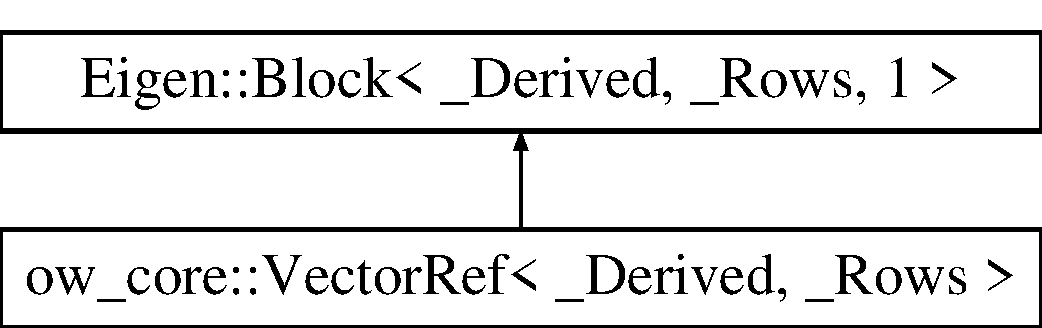
\includegraphics[height=2.000000cm]{de/d6a/classow__core_1_1VectorRef}
\end{center}
\end{figure}
\subsection*{Public Types}
\begin{DoxyCompactItemize}
\item 
enum \{ {\bfseries Rows} = \+\_\+\+Rows
 \}\hypertarget{classow__core_1_1VectorRef_a1fece9813818a7e76b4d602544b9459d}{}\label{classow__core_1_1VectorRef_a1fece9813818a7e76b4d602544b9459d}

\item 
typedef \+\_\+\+Derived {\bfseries Derived}\hypertarget{classow__core_1_1VectorRef_a7536251477ddb12a8c69099b2bd927f2}{}\label{classow__core_1_1VectorRef_a7536251477ddb12a8c69099b2bd927f2}

\item 
typedef Eigen\+::\+Block$<$ Derived, Rows, 1 $>$ {\bfseries Base}\hypertarget{classow__core_1_1VectorRef_a279d56c9662da5a4fbc798e5d554c273}{}\label{classow__core_1_1VectorRef_a279d56c9662da5a4fbc798e5d554c273}

\end{DoxyCompactItemize}
\subsection*{Public Member Functions}
\begin{DoxyCompactItemize}
\item 
\hyperlink{classow__core_1_1VectorRef_add9b005be63c7346b39ddf869e591b4b}{Vector\+Ref} (Derived \&ref, int start\+Row=0, int start\+Col=0)
\begin{DoxyCompactList}\small\item\em Default Constructor. \end{DoxyCompactList}\item 
std\+::string \hyperlink{classow__core_1_1VectorRef_a8801753aee0b11331a4613f5d3391afc}{to\+String} () const \hypertarget{classow__core_1_1VectorRef_a8801753aee0b11331a4613f5d3391afc}{}\label{classow__core_1_1VectorRef_a8801753aee0b11331a4613f5d3391afc}

\begin{DoxyCompactList}\small\item\em Conversion to std\+::string. \end{DoxyCompactList}\end{DoxyCompactItemize}


\subsection{Detailed Description}
\subsubsection*{template$<$typename \+\_\+\+Derived, int \+\_\+\+Rows$>$\\*
class ow\+\_\+core\+::\+Vector\+Ref$<$ \+\_\+\+Derived, \+\_\+\+Rows $>$}

The \hyperlink{classow__core_1_1VectorRef}{Vector\+Ref} class. 

References the data of another Eigen type class via Eigen\+:Block.

We need this special type to get the behavior of Eigen\+::\+Matrix when defining new references. 

\subsection{Constructor \& Destructor Documentation}
\index{ow\+\_\+core\+::\+Vector\+Ref@{ow\+\_\+core\+::\+Vector\+Ref}!Vector\+Ref@{Vector\+Ref}}
\index{Vector\+Ref@{Vector\+Ref}!ow\+\_\+core\+::\+Vector\+Ref@{ow\+\_\+core\+::\+Vector\+Ref}}
\subsubsection[{\texorpdfstring{Vector\+Ref(\+Derived \&ref, int start\+Row=0, int start\+Col=0)}{VectorRef(Derived &ref, int startRow=0, int startCol=0)}}]{\setlength{\rightskip}{0pt plus 5cm}template$<$typename \+\_\+\+Derived, int \+\_\+\+Rows$>$ {\bf ow\+\_\+core\+::\+Vector\+Ref}$<$ \+\_\+\+Derived, \+\_\+\+Rows $>$\+::{\bf Vector\+Ref} (
\begin{DoxyParamCaption}
\item[{Derived \&}]{ref, }
\item[{int}]{start\+Row = {\ttfamily 0}, }
\item[{int}]{start\+Col = {\ttfamily 0}}
\end{DoxyParamCaption}
)\hspace{0.3cm}{\ttfamily [inline]}, {\ttfamily [explicit]}}\hypertarget{classow__core_1_1VectorRef_add9b005be63c7346b39ddf869e591b4b}{}\label{classow__core_1_1VectorRef_add9b005be63c7346b39ddf869e591b4b}


Default Constructor. 


\begin{DoxyParams}{Parameters}
{\em ref} & the reference to storage Eigen object to access the elements of the quaternion via Eigen\+::\+Block.\\
\hline
{\em start\+Row} & the start index of the row for Eigen\+::\+Block.\\
\hline
{\em start\+Col} & the start index of the column for Eigen\+::\+Block. \\
\hline
\end{DoxyParams}


The documentation for this class was generated from the following file\+:\begin{DoxyCompactItemize}
\item 
/home/dean/ros/workspaces/ow\+\_\+test\+\_\+ws/src/ow\+\_\+core/include/ow\+\_\+core/\hyperlink{vector__ref_8h}{vector\+\_\+ref.\+h}\end{DoxyCompactItemize}

\hypertarget{classow__core_1_1Wrench}{}\section{ow\+\_\+core\+:\+:Wrench$<$ \+\_\+\+Scalar $>$ Class Template Reference}
\label{classow__core_1_1Wrench}\index{ow\+\_\+core\+::\+Wrench$<$ \+\_\+\+Scalar $>$@{ow\+\_\+core\+::\+Wrench$<$ \+\_\+\+Scalar $>$}}


The \hyperlink{classow__core_1_1Wrench}{Wrench} class.  




{\ttfamily \#include $<$wrench.\+h$>$}

Inheritance diagram for ow\+\_\+core\+:\+:Wrench$<$ \+\_\+\+Scalar $>$\+:\begin{figure}[H]
\begin{center}
\leavevmode
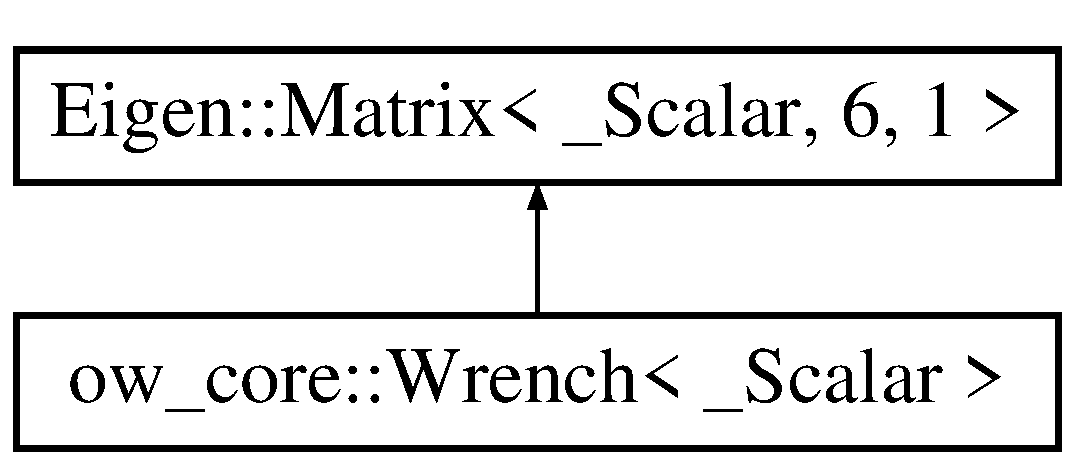
\includegraphics[height=2.000000cm]{dc/dd9/classow__core_1_1Wrench}
\end{center}
\end{figure}
\subsection*{Public Types}
\begin{DoxyCompactItemize}
\item 
typedef \+\_\+\+Scalar {\bfseries Scalar}\hypertarget{classow__core_1_1Wrench_af462e5302ef95be5f70d5a7889c994ca}{}\label{classow__core_1_1Wrench_af462e5302ef95be5f70d5a7889c994ca}

\item 
typedef Eigen\+::\+Matrix$<$ Scalar, 6, 1 $>$ {\bfseries Base}\hypertarget{classow__core_1_1Wrench_a493b8a5d84ade9788815b5967f67774a}{}\label{classow__core_1_1Wrench_a493b8a5d84ade9788815b5967f67774a}

\end{DoxyCompactItemize}
\subsection*{Public Member Functions}
\begin{DoxyCompactItemize}
\item 
\hyperlink{classow__core_1_1Wrench_a3b052077efbd8a5029346ffb3507ab92}{Wrench} ()\hypertarget{classow__core_1_1Wrench_a3b052077efbd8a5029346ffb3507ab92}{}\label{classow__core_1_1Wrench_a3b052077efbd8a5029346ffb3507ab92}

\begin{DoxyCompactList}\small\item\em Default Constructor. \end{DoxyCompactList}\item 
{\footnotesize template$<$typename Other\+Derived $>$ }\\\hyperlink{classow__core_1_1Wrench_a78e79150a8f7377ff4cb9be4f203a20d}{Wrench} (const Eigen\+::\+Eigen\+Base$<$ Other\+Derived $>$ \&other)
\begin{DoxyCompactList}\small\item\em Copy constructor. \end{DoxyCompactList}\item 
\hyperlink{classow__core_1_1Wrench_a57d2dfb70214e79f720d064124a8e102}{Wrench} (const geometry\+\_\+msgs\+::\+Wrench \&other)\hypertarget{classow__core_1_1Wrench_a57d2dfb70214e79f720d064124a8e102}{}\label{classow__core_1_1Wrench_a57d2dfb70214e79f720d064124a8e102}

\begin{DoxyCompactList}\small\item\em Copy constructor form geometry\+\_\+msgs\+::\+Wrench. \end{DoxyCompactList}\item 
void \hyperlink{classow__core_1_1Wrench_a8fcbb87b2ff0e2c7742def7ac08903ba}{operator=} (const geometry\+\_\+msgs\+::\+Wrench \&W)\hypertarget{classow__core_1_1Wrench_a8fcbb87b2ff0e2c7742def7ac08903ba}{}\label{classow__core_1_1Wrench_a8fcbb87b2ff0e2c7742def7ac08903ba}

\begin{DoxyCompactList}\small\item\em Assignment form geometry\+\_\+msgs\+::\+Wrench. \end{DoxyCompactList}\item 
\hyperlink{classow__core_1_1Wrench_a08aa041f5fc3fbe34dbede0807d10e1e}{operator geometry\+\_\+msgs\+::\+Wrench} () const \hypertarget{classow__core_1_1Wrench_a08aa041f5fc3fbe34dbede0807d10e1e}{}\label{classow__core_1_1Wrench_a08aa041f5fc3fbe34dbede0807d10e1e}

\begin{DoxyCompactList}\small\item\em Conversion to geometry\+\_\+msgs\+::\+Twist. \end{DoxyCompactList}\item 
geometry\+\_\+msgs\+::\+Wrench \hyperlink{classow__core_1_1Wrench_a304d746f248d1503c41c3dde2d4bb674}{to\+Wrench\+Msg} () const \hypertarget{classow__core_1_1Wrench_a304d746f248d1503c41c3dde2d4bb674}{}\label{classow__core_1_1Wrench_a304d746f248d1503c41c3dde2d4bb674}

\begin{DoxyCompactList}\small\item\em Conversion to geometry\+\_\+msgs\+::\+Twist. \end{DoxyCompactList}\item 
\hyperlink{classow__core_1_1ForceRef}{Force\+Ref}$<$ Base $>$ \hyperlink{classow__core_1_1Wrench_a1280c591f4fc192916f6398d92074870}{force} ()\hypertarget{classow__core_1_1Wrench_a1280c591f4fc192916f6398d92074870}{}\label{classow__core_1_1Wrench_a1280c591f4fc192916f6398d92074870}

\begin{DoxyCompactList}\small\item\em access to linear part \end{DoxyCompactList}\item 
\hyperlink{classow__core_1_1ForceRef}{Force\+Ref}$<$ const Base $>$ \hyperlink{classow__core_1_1Wrench_a4e8dce56464223a729052e6ad83dbe52}{force} () const \hypertarget{classow__core_1_1Wrench_a4e8dce56464223a729052e6ad83dbe52}{}\label{classow__core_1_1Wrench_a4e8dce56464223a729052e6ad83dbe52}

\begin{DoxyCompactList}\small\item\em const access to linear part \end{DoxyCompactList}\item 
\hyperlink{classow__core_1_1MomentRef}{Moment\+Ref}$<$ Base $>$ \hyperlink{classow__core_1_1Wrench_a8ce23dd81a3aaffc0298531f785647de}{moment} ()\hypertarget{classow__core_1_1Wrench_a8ce23dd81a3aaffc0298531f785647de}{}\label{classow__core_1_1Wrench_a8ce23dd81a3aaffc0298531f785647de}

\begin{DoxyCompactList}\small\item\em access to angular part \end{DoxyCompactList}\item 
\hyperlink{classow__core_1_1MomentRef}{Moment\+Ref}$<$ const Base $>$ \hyperlink{classow__core_1_1Wrench_a2cddfa50e6078ff59f3bbcbb36bace2d}{moment} () const \hypertarget{classow__core_1_1Wrench_a2cddfa50e6078ff59f3bbcbb36bace2d}{}\label{classow__core_1_1Wrench_a2cddfa50e6078ff59f3bbcbb36bace2d}

\begin{DoxyCompactList}\small\item\em const access to angular part \end{DoxyCompactList}\item 
std\+::string \hyperlink{classow__core_1_1Wrench_a5b9957b13debc043deab64b5f5467504}{to\+String} () const \hypertarget{classow__core_1_1Wrench_a5b9957b13debc043deab64b5f5467504}{}\label{classow__core_1_1Wrench_a5b9957b13debc043deab64b5f5467504}

\begin{DoxyCompactList}\small\item\em Conversion to std\+::string. \end{DoxyCompactList}\end{DoxyCompactItemize}
\subsection*{Static Public Member Functions}
\begin{DoxyCompactItemize}
\item 
static const \hyperlink{classow__core_1_1Wrench}{Wrench} \& \hyperlink{classow__core_1_1Wrench_a3dc8f10073ab93f15eb839b2a0fef07e}{Default} ()
\begin{DoxyCompactList}\small\item\em Construct as Default. \end{DoxyCompactList}\end{DoxyCompactItemize}


\subsection{Detailed Description}
\subsubsection*{template$<$typename \+\_\+\+Scalar$>$\\*
class ow\+\_\+core\+::\+Wrench$<$ \+\_\+\+Scalar $>$}

The \hyperlink{classow__core_1_1Wrench}{Wrench} class. 

The \hyperlink{classow__core_1_1Wrench}{Wrench} is of type Eigen\+::\+Vector6 and is represented by the math symbol $\mathbf{W}$.

Stores the force and moment in a 6 dimensional vector. The force is represented by the first three elements. The moment velocity by the last three elements. 

\subsection{Constructor \& Destructor Documentation}
\index{ow\+\_\+core\+::\+Wrench@{ow\+\_\+core\+::\+Wrench}!Wrench@{Wrench}}
\index{Wrench@{Wrench}!ow\+\_\+core\+::\+Wrench@{ow\+\_\+core\+::\+Wrench}}
\subsubsection[{\texorpdfstring{Wrench(const Eigen\+::\+Eigen\+Base$<$ Other\+Derived $>$ \&other)}{Wrench(const Eigen::EigenBase< OtherDerived > &other)}}]{\setlength{\rightskip}{0pt plus 5cm}template$<$typename \+\_\+\+Scalar$>$ template$<$typename Other\+Derived $>$ {\bf ow\+\_\+core\+::\+Wrench}$<$ \+\_\+\+Scalar $>$\+::{\bf Wrench} (
\begin{DoxyParamCaption}
\item[{const Eigen\+::\+Eigen\+Base$<$ Other\+Derived $>$ \&}]{other}
\end{DoxyParamCaption}
)\hspace{0.3cm}{\ttfamily [inline]}}\hypertarget{classow__core_1_1Wrench_a78e79150a8f7377ff4cb9be4f203a20d}{}\label{classow__core_1_1Wrench_a78e79150a8f7377ff4cb9be4f203a20d}


Copy constructor. 

This copy constructor not only works with Eigen matrices but also with their expressions. 

\subsection{Member Function Documentation}
\index{ow\+\_\+core\+::\+Wrench@{ow\+\_\+core\+::\+Wrench}!Default@{Default}}
\index{Default@{Default}!ow\+\_\+core\+::\+Wrench@{ow\+\_\+core\+::\+Wrench}}
\subsubsection[{\texorpdfstring{Default()}{Default()}}]{\setlength{\rightskip}{0pt plus 5cm}template$<$typename \+\_\+\+Scalar$>$ static const {\bf Wrench}\& {\bf ow\+\_\+core\+::\+Wrench}$<$ \+\_\+\+Scalar $>$\+::Default (
\begin{DoxyParamCaption}
{}
\end{DoxyParamCaption}
)\hspace{0.3cm}{\ttfamily [inline]}, {\ttfamily [static]}}\hypertarget{classow__core_1_1Wrench_a3dc8f10073ab93f15eb839b2a0fef07e}{}\label{classow__core_1_1Wrench_a3dc8f10073ab93f15eb839b2a0fef07e}


Construct as Default. 

Default is Zero. 

The documentation for this class was generated from the following file\+:\begin{DoxyCompactItemize}
\item 
/home/dean/ros/workspaces/ow\+\_\+test\+\_\+ws/src/ow\+\_\+core/include/ow\+\_\+core/\hyperlink{wrench_8h}{wrench.\+h}\end{DoxyCompactItemize}

\chapter{File Documentation}
\hypertarget{angular__acceleration_8h}{}\section{/home/dean/ros/workspaces/ow\+\_\+test\+\_\+ws/src/ow\+\_\+core/include/ow\+\_\+core/angular\+\_\+acceleration.h File Reference}
\label{angular__acceleration_8h}\index{/home/dean/ros/workspaces/ow\+\_\+test\+\_\+ws/src/ow\+\_\+core/include/ow\+\_\+core/angular\+\_\+acceleration.\+h@{/home/dean/ros/workspaces/ow\+\_\+test\+\_\+ws/src/ow\+\_\+core/include/ow\+\_\+core/angular\+\_\+acceleration.\+h}}
{\ttfamily \#include $<$ow\+\_\+core/angular\+\_\+acceleration\+\_\+ref.\+h$>$}\\*
\subsection*{Classes}
\begin{DoxyCompactItemize}
\item 
class \hyperlink{classow__core_1_1AngularAcceleration}{ow\+\_\+core\+::\+Angular\+Acceleration$<$ \+\_\+\+Scalar $>$}
\begin{DoxyCompactList}\small\item\em The \hyperlink{classow__core_1_1AngularAcceleration}{Angular\+Acceleration} class. \end{DoxyCompactList}\end{DoxyCompactItemize}


\subsection{Detailed Description}
\begin{DoxyAuthor}{Author}
Emmanuel Dean-\/\+Leon 

Florian Bergner 

J. Rogelio Guadarrama-\/\+Olvera 

Simon Armleder 

Gordon Cheng
\end{DoxyAuthor}
\begin{DoxyVersion}{Version}
0.\+1 
\end{DoxyVersion}
\begin{DoxyDate}{Date}
14.\+02.\+2020
\end{DoxyDate}
\begin{DoxyCopyright}{Copyright}
Copyright 2020 Institute for Cognitive Systems (I\+CS), Technical University of Munich (T\+UM)
\end{DoxyCopyright}
\subparagraph*{Licence}

Licensed under the Apache License, Version 2.\+0 (the \char`\"{}\+License\char`\"{}); you may not use this file except in compliance with the License. You may obtain a copy of the License at

\href{http://www.apache.org/licenses/LICENSE-2.0}{\tt http\+://www.\+apache.\+org/licenses/\+L\+I\+C\+E\+N\+S\+E-\/2.\+0}

Unless required by applicable law or agreed to in writing, software distributed under the License is distributed on an \char`\"{}\+A\+S I\+S\char`\"{} B\+A\+S\+IS, W\+I\+T\+H\+O\+UT W\+A\+R\+R\+A\+N\+T\+I\+ES OR C\+O\+N\+D\+I\+T\+I\+O\+NS OF A\+NY K\+I\+ND, either express or implied. See the License for the specific language governing permissions and limitations under the License.

\subparagraph*{Acknowledgment}

This project has received funding from the European Union‘s Horizon 2020 research and innovation programme under grant agreement No 732287. 
\hypertarget{angular__acceleration__ref_8h}{}\section{/home/dean/ros/workspaces/ow\+\_\+test\+\_\+ws/src/ow\+\_\+core/include/ow\+\_\+core/angular\+\_\+acceleration\+\_\+ref.h File Reference}
\label{angular__acceleration__ref_8h}\index{/home/dean/ros/workspaces/ow\+\_\+test\+\_\+ws/src/ow\+\_\+core/include/ow\+\_\+core/angular\+\_\+acceleration\+\_\+ref.\+h@{/home/dean/ros/workspaces/ow\+\_\+test\+\_\+ws/src/ow\+\_\+core/include/ow\+\_\+core/angular\+\_\+acceleration\+\_\+ref.\+h}}
{\ttfamily \#include $<$ow\+\_\+core/vector3\+\_\+ref.\+h$>$}\\*
\subsection*{Classes}
\begin{DoxyCompactItemize}
\item 
class \hyperlink{classow__core_1_1AngularAccelerationRef}{ow\+\_\+core\+::\+Angular\+Acceleration\+Ref$<$ \+\_\+\+Derived $>$}
\begin{DoxyCompactList}\small\item\em The \hyperlink{classow__core_1_1AngularAccelerationRef}{Angular\+Acceleration\+Ref} class. \end{DoxyCompactList}\end{DoxyCompactItemize}


\subsection{Detailed Description}
\begin{DoxyAuthor}{Author}
Emmanuel Dean-\/\+Leon 

Florian Bergner 

J. Rogelio Guadarrama-\/\+Olvera 

Simon Armleder 

Gordon Cheng
\end{DoxyAuthor}
\begin{DoxyVersion}{Version}
0.\+1 
\end{DoxyVersion}
\begin{DoxyDate}{Date}
14.\+02.\+2020
\end{DoxyDate}
\begin{DoxyCopyright}{Copyright}
Copyright 2020 Institute for Cognitive Systems (I\+CS), Technical University of Munich (T\+UM)
\end{DoxyCopyright}
\subparagraph*{Licence}

Licensed under the Apache License, Version 2.\+0 (the \char`\"{}\+License\char`\"{}); you may not use this file except in compliance with the License. You may obtain a copy of the License at

\href{http://www.apache.org/licenses/LICENSE-2.0}{\tt http\+://www.\+apache.\+org/licenses/\+L\+I\+C\+E\+N\+S\+E-\/2.\+0}

Unless required by applicable law or agreed to in writing, software distributed under the License is distributed on an \char`\"{}\+A\+S I\+S\char`\"{} B\+A\+S\+IS, W\+I\+T\+H\+O\+UT W\+A\+R\+R\+A\+N\+T\+I\+ES OR C\+O\+N\+D\+I\+T\+I\+O\+NS OF A\+NY K\+I\+ND, either express or implied. See the License for the specific language governing permissions and limitations under the License.

\subparagraph*{Acknowledgment}

This project has received funding from the European Union‘s Horizon 2020 research and innovation programme under grant agreement No 732287. 
\hypertarget{angular__position_8h}{}\section{/home/dean/ros/workspaces/ow\+\_\+test\+\_\+ws/src/ow\+\_\+core/include/ow\+\_\+core/angular\+\_\+position.h File Reference}
\label{angular__position_8h}\index{/home/dean/ros/workspaces/ow\+\_\+test\+\_\+ws/src/ow\+\_\+core/include/ow\+\_\+core/angular\+\_\+position.\+h@{/home/dean/ros/workspaces/ow\+\_\+test\+\_\+ws/src/ow\+\_\+core/include/ow\+\_\+core/angular\+\_\+position.\+h}}
{\ttfamily \#include $<$ow\+\_\+core/conversions.\+h$>$}\\*
{\ttfamily \#include $<$ow\+\_\+core/angular\+\_\+position\+\_\+ref.\+h$>$}\\*
\subsection*{Classes}
\begin{DoxyCompactItemize}
\item 
class \hyperlink{classow__core_1_1AngularPosition}{ow\+\_\+core\+::\+Angular\+Position$<$ \+\_\+\+Scalar $>$}
\begin{DoxyCompactList}\small\item\em The \hyperlink{classow__core_1_1AngularPosition}{Angular\+Position} class. \end{DoxyCompactList}\end{DoxyCompactItemize}


\subsection{Detailed Description}
\begin{DoxyAuthor}{Author}
Emmanuel Dean-\/\+Leon 

Florian Bergner 

J. Rogelio Guadarrama-\/\+Olvera 

Simon Armleder 

Gordon Cheng
\end{DoxyAuthor}
\begin{DoxyVersion}{Version}
0.\+1 
\end{DoxyVersion}
\begin{DoxyDate}{Date}
14.\+02.\+2020
\end{DoxyDate}
\begin{DoxyCopyright}{Copyright}
Copyright 2020 Institute for Cognitive Systems (I\+CS), Technical University of Munich (T\+UM)
\end{DoxyCopyright}
\subparagraph*{Licence}

Licensed under the Apache License, Version 2.\+0 (the \char`\"{}\+License\char`\"{}); you may not use this file except in compliance with the License. You may obtain a copy of the License at

\href{http://www.apache.org/licenses/LICENSE-2.0}{\tt http\+://www.\+apache.\+org/licenses/\+L\+I\+C\+E\+N\+S\+E-\/2.\+0}

Unless required by applicable law or agreed to in writing, software distributed under the License is distributed on an \char`\"{}\+A\+S I\+S\char`\"{} B\+A\+S\+IS, W\+I\+T\+H\+O\+UT W\+A\+R\+R\+A\+N\+T\+I\+ES OR C\+O\+N\+D\+I\+T\+I\+O\+NS OF A\+NY K\+I\+ND, either express or implied. See the License for the specific language governing permissions and limitations under the License.

\subparagraph*{Acknowledgment}

This project has received funding from the European Union‘s Horizon 2020 research and innovation programme under grant agreement No 732287. 
\hypertarget{angular__position__ref_8h}{}\section{/home/dean/ros/workspaces/ow\+\_\+test\+\_\+ws/src/ow\+\_\+core/include/ow\+\_\+core/angular\+\_\+position\+\_\+ref.h File Reference}
\label{angular__position__ref_8h}\index{/home/dean/ros/workspaces/ow\+\_\+test\+\_\+ws/src/ow\+\_\+core/include/ow\+\_\+core/angular\+\_\+position\+\_\+ref.\+h@{/home/dean/ros/workspaces/ow\+\_\+test\+\_\+ws/src/ow\+\_\+core/include/ow\+\_\+core/angular\+\_\+position\+\_\+ref.\+h}}
{\ttfamily \#include $<$ow\+\_\+core/conversions.\+h$>$}\\*
{\ttfamily \#include $<$ow\+\_\+core/quaternion\+\_\+ref.\+h$>$}\\*
\subsection*{Classes}
\begin{DoxyCompactItemize}
\item 
class \hyperlink{classow__core_1_1AngularPositionRef}{ow\+\_\+core\+::\+Angular\+Position\+Ref$<$ \+\_\+\+Derived $>$}
\begin{DoxyCompactList}\small\item\em The \hyperlink{classow__core_1_1AngularPositionRef}{Angular\+Position\+Ref} class. \end{DoxyCompactList}\end{DoxyCompactItemize}


\subsection{Detailed Description}
\begin{DoxyAuthor}{Author}
Emmanuel Dean-\/\+Leon 

Florian Bergner 

J. Rogelio Guadarrama-\/\+Olvera 

Simon Armleder 

Gordon Cheng
\end{DoxyAuthor}
\begin{DoxyVersion}{Version}
0.\+1 
\end{DoxyVersion}
\begin{DoxyDate}{Date}
14.\+02.\+2020
\end{DoxyDate}
\begin{DoxyCopyright}{Copyright}
Copyright 2020 Institute for Cognitive Systems (I\+CS), Technical University of Munich (T\+UM)
\end{DoxyCopyright}
\subparagraph*{Licence}

Licensed under the Apache License, Version 2.\+0 (the \char`\"{}\+License\char`\"{}); you may not use this file except in compliance with the License. You may obtain a copy of the License at

\href{http://www.apache.org/licenses/LICENSE-2.0}{\tt http\+://www.\+apache.\+org/licenses/\+L\+I\+C\+E\+N\+S\+E-\/2.\+0}

Unless required by applicable law or agreed to in writing, software distributed under the License is distributed on an \char`\"{}\+A\+S I\+S\char`\"{} B\+A\+S\+IS, W\+I\+T\+H\+O\+UT W\+A\+R\+R\+A\+N\+T\+I\+ES OR C\+O\+N\+D\+I\+T\+I\+O\+NS OF A\+NY K\+I\+ND, either express or implied. See the License for the specific language governing permissions and limitations under the License.

\subparagraph*{Acknowledgment}

This project has received funding from the European Union‘s Horizon 2020 research and innovation programme under grant agreement No 732287. 
\hypertarget{angular__velocity_8h}{}\section{/home/dean/ros/workspaces/ow\+\_\+test\+\_\+ws/src/ow\+\_\+core/include/ow\+\_\+core/angular\+\_\+velocity.h File Reference}
\label{angular__velocity_8h}\index{/home/dean/ros/workspaces/ow\+\_\+test\+\_\+ws/src/ow\+\_\+core/include/ow\+\_\+core/angular\+\_\+velocity.\+h@{/home/dean/ros/workspaces/ow\+\_\+test\+\_\+ws/src/ow\+\_\+core/include/ow\+\_\+core/angular\+\_\+velocity.\+h}}
{\ttfamily \#include $<$ow\+\_\+core/angular\+\_\+velocity\+\_\+ref.\+h$>$}\\*
\subsection*{Classes}
\begin{DoxyCompactItemize}
\item 
class \hyperlink{classow__core_1_1AngularVelocity}{ow\+\_\+core\+::\+Angular\+Velocity$<$ \+\_\+\+Scalar $>$}
\begin{DoxyCompactList}\small\item\em The \hyperlink{classow__core_1_1AngularVelocity}{Angular\+Velocity} class. \end{DoxyCompactList}\end{DoxyCompactItemize}


\subsection{Detailed Description}
\begin{DoxyAuthor}{Author}
Emmanuel Dean-\/\+Leon 

Florian Bergner 

J. Rogelio Guadarrama-\/\+Olvera 

Simon Armleder 

Gordon Cheng
\end{DoxyAuthor}
\begin{DoxyVersion}{Version}
0.\+1 
\end{DoxyVersion}
\begin{DoxyDate}{Date}
14.\+02.\+2020
\end{DoxyDate}
\begin{DoxyCopyright}{Copyright}
Copyright 2020 Institute for Cognitive Systems (I\+CS), Technical University of Munich (T\+UM)
\end{DoxyCopyright}
\subparagraph*{Licence}

Licensed under the Apache License, Version 2.\+0 (the \char`\"{}\+License\char`\"{}); you may not use this file except in compliance with the License. You may obtain a copy of the License at

\href{http://www.apache.org/licenses/LICENSE-2.0}{\tt http\+://www.\+apache.\+org/licenses/\+L\+I\+C\+E\+N\+S\+E-\/2.\+0}

Unless required by applicable law or agreed to in writing, software distributed under the License is distributed on an \char`\"{}\+A\+S I\+S\char`\"{} B\+A\+S\+IS, W\+I\+T\+H\+O\+UT W\+A\+R\+R\+A\+N\+T\+I\+ES OR C\+O\+N\+D\+I\+T\+I\+O\+NS OF A\+NY K\+I\+ND, either express or implied. See the License for the specific language governing permissions and limitations under the License.

\subparagraph*{Acknowledgment}

This project has received funding from the European Union‘s Horizon 2020 research and innovation programme under grant agreement No 732287. 
\hypertarget{angular__velocity__ref_8h}{}\section{/home/dean/ros/workspaces/ow\+\_\+test\+\_\+ws/src/ow\+\_\+core/include/ow\+\_\+core/angular\+\_\+velocity\+\_\+ref.h File Reference}
\label{angular__velocity__ref_8h}\index{/home/dean/ros/workspaces/ow\+\_\+test\+\_\+ws/src/ow\+\_\+core/include/ow\+\_\+core/angular\+\_\+velocity\+\_\+ref.\+h@{/home/dean/ros/workspaces/ow\+\_\+test\+\_\+ws/src/ow\+\_\+core/include/ow\+\_\+core/angular\+\_\+velocity\+\_\+ref.\+h}}
{\ttfamily \#include $<$ow\+\_\+core/vector3\+\_\+ref.\+h$>$}\\*
\subsection*{Classes}
\begin{DoxyCompactItemize}
\item 
class \hyperlink{classow__core_1_1AngularVelocityRef}{ow\+\_\+core\+::\+Angular\+Velocity\+Ref$<$ \+\_\+\+Derived $>$}
\begin{DoxyCompactList}\small\item\em The \hyperlink{classow__core_1_1AngularVelocityRef}{Angular\+Velocity\+Ref} class. \end{DoxyCompactList}\end{DoxyCompactItemize}


\subsection{Detailed Description}
\begin{DoxyAuthor}{Author}
Emmanuel Dean-\/\+Leon 

Florian Bergner 

J. Rogelio Guadarrama-\/\+Olvera 

Simon Armleder 

Gordon Cheng
\end{DoxyAuthor}
\begin{DoxyVersion}{Version}
0.\+1 
\end{DoxyVersion}
\begin{DoxyDate}{Date}
14.\+02.\+2020
\end{DoxyDate}
\begin{DoxyCopyright}{Copyright}
Copyright 2020 Institute for Cognitive Systems (I\+CS), Technical University of Munich (T\+UM)
\end{DoxyCopyright}
\subparagraph*{Licence}

Licensed under the Apache License, Version 2.\+0 (the \char`\"{}\+License\char`\"{}); you may not use this file except in compliance with the License. You may obtain a copy of the License at

\href{http://www.apache.org/licenses/LICENSE-2.0}{\tt http\+://www.\+apache.\+org/licenses/\+L\+I\+C\+E\+N\+S\+E-\/2.\+0}

Unless required by applicable law or agreed to in writing, software distributed under the License is distributed on an \char`\"{}\+A\+S I\+S\char`\"{} B\+A\+S\+IS, W\+I\+T\+H\+O\+UT W\+A\+R\+R\+A\+N\+T\+I\+ES OR C\+O\+N\+D\+I\+T\+I\+O\+NS OF A\+NY K\+I\+ND, either express or implied. See the License for the specific language governing permissions and limitations under the License.

\subparagraph*{Acknowledgment}

This project has received funding from the European Union‘s Horizon 2020 research and innovation programme under grant agreement No 732287. 
\hypertarget{cartesian__acceleration_8h}{}\section{/home/dean/ros/workspaces/ow\+\_\+test\+\_\+ws/src/ow\+\_\+core/include/ow\+\_\+core/cartesian\+\_\+acceleration.h File Reference}
\label{cartesian__acceleration_8h}\index{/home/dean/ros/workspaces/ow\+\_\+test\+\_\+ws/src/ow\+\_\+core/include/ow\+\_\+core/cartesian\+\_\+acceleration.\+h@{/home/dean/ros/workspaces/ow\+\_\+test\+\_\+ws/src/ow\+\_\+core/include/ow\+\_\+core/cartesian\+\_\+acceleration.\+h}}
{\ttfamily \#include $<$ow\+\_\+core/linear\+\_\+acceleration\+\_\+ref.\+h$>$}\\*
{\ttfamily \#include $<$ow\+\_\+core/angular\+\_\+acceleration\+\_\+ref.\+h$>$}\\*
{\ttfamily \#include $<$geometry\+\_\+msgs/\+Accel.\+h$>$}\\*
\subsection*{Classes}
\begin{DoxyCompactItemize}
\item 
class \hyperlink{classow__core_1_1CartesianAcceleration}{ow\+\_\+core\+::\+Cartesian\+Acceleration$<$ \+\_\+\+Scalar $>$}
\begin{DoxyCompactList}\small\item\em The \hyperlink{classow__core_1_1CartesianAcceleration}{Cartesian\+Acceleration} class. \end{DoxyCompactList}\end{DoxyCompactItemize}


\subsection{Detailed Description}
\begin{DoxyAuthor}{Author}
Emmanuel Dean-\/\+Leon 

Florian Bergner 

J. Rogelio Guadarrama-\/\+Olvera 

Simon Armleder 

Gordon Cheng
\end{DoxyAuthor}
\begin{DoxyVersion}{Version}
0.\+1 
\end{DoxyVersion}
\begin{DoxyDate}{Date}
14.\+02.\+2020
\end{DoxyDate}
\begin{DoxyCopyright}{Copyright}
Copyright 2020 Institute for Cognitive Systems (I\+CS), Technical University of Munich (T\+UM)
\end{DoxyCopyright}
\subparagraph*{Licence}

Licensed under the Apache License, Version 2.\+0 (the \char`\"{}\+License\char`\"{}); you may not use this file except in compliance with the License. You may obtain a copy of the License at

\href{http://www.apache.org/licenses/LICENSE-2.0}{\tt http\+://www.\+apache.\+org/licenses/\+L\+I\+C\+E\+N\+S\+E-\/2.\+0}

Unless required by applicable law or agreed to in writing, software distributed under the License is distributed on an \char`\"{}\+A\+S I\+S\char`\"{} B\+A\+S\+IS, W\+I\+T\+H\+O\+UT W\+A\+R\+R\+A\+N\+T\+I\+ES OR C\+O\+N\+D\+I\+T\+I\+O\+NS OF A\+NY K\+I\+ND, either express or implied. See the License for the specific language governing permissions and limitations under the License.

\subparagraph*{Acknowledgment}

This project has received funding from the European Union‘s Horizon 2020 research and innovation programme under grant agreement No 732287. 
\hypertarget{cartesian__position_8h}{}\section{/home/dean/ros/workspaces/ow\+\_\+test\+\_\+ws/src/ow\+\_\+core/include/ow\+\_\+core/cartesian\+\_\+position.h File Reference}
\label{cartesian__position_8h}\index{/home/dean/ros/workspaces/ow\+\_\+test\+\_\+ws/src/ow\+\_\+core/include/ow\+\_\+core/cartesian\+\_\+position.\+h@{/home/dean/ros/workspaces/ow\+\_\+test\+\_\+ws/src/ow\+\_\+core/include/ow\+\_\+core/cartesian\+\_\+position.\+h}}
{\ttfamily \#include $<$ow\+\_\+core/angular\+\_\+position\+\_\+ref.\+h$>$}\\*
{\ttfamily \#include $<$ow\+\_\+core/linear\+\_\+position\+\_\+ref.\+h$>$}\\*
{\ttfamily \#include $<$geometry\+\_\+msgs/\+Pose.\+h$>$}\\*
\subsection*{Classes}
\begin{DoxyCompactItemize}
\item 
class \hyperlink{classow__core_1_1CartesianPosition}{ow\+\_\+core\+::\+Cartesian\+Position$<$ \+\_\+\+Scalar $>$}
\begin{DoxyCompactList}\small\item\em The \hyperlink{classow__core_1_1CartesianPosition}{Cartesian\+Position} class. \end{DoxyCompactList}\end{DoxyCompactItemize}


\subsection{Detailed Description}
\begin{DoxyAuthor}{Author}
Emmanuel Dean-\/\+Leon 

Florian Bergner 

J. Rogelio Guadarrama-\/\+Olvera 

Simon Armleder 

Gordon Cheng
\end{DoxyAuthor}
\begin{DoxyVersion}{Version}
0.\+1 
\end{DoxyVersion}
\begin{DoxyDate}{Date}
14.\+02.\+2020
\end{DoxyDate}
\begin{DoxyCopyright}{Copyright}
Copyright 2020 Institute for Cognitive Systems (I\+CS), Technical University of Munich (T\+UM)
\end{DoxyCopyright}
\subparagraph*{Licence}

Licensed under the Apache License, Version 2.\+0 (the \char`\"{}\+License\char`\"{}); you may not use this file except in compliance with the License. You may obtain a copy of the License at

\href{http://www.apache.org/licenses/LICENSE-2.0}{\tt http\+://www.\+apache.\+org/licenses/\+L\+I\+C\+E\+N\+S\+E-\/2.\+0}

Unless required by applicable law or agreed to in writing, software distributed under the License is distributed on an \char`\"{}\+A\+S I\+S\char`\"{} B\+A\+S\+IS, W\+I\+T\+H\+O\+UT W\+A\+R\+R\+A\+N\+T\+I\+ES OR C\+O\+N\+D\+I\+T\+I\+O\+NS OF A\+NY K\+I\+ND, either express or implied. See the License for the specific language governing permissions and limitations under the License.

\subparagraph*{Acknowledgment}

This project has received funding from the European Union‘s Horizon 2020 research and innovation programme under grant agreement No 732287. 
\hypertarget{cartesian__velocity_8h}{}\section{/home/dean/ros/workspaces/ow\+\_\+test\+\_\+ws/src/ow\+\_\+core/include/ow\+\_\+core/cartesian\+\_\+velocity.h File Reference}
\label{cartesian__velocity_8h}\index{/home/dean/ros/workspaces/ow\+\_\+test\+\_\+ws/src/ow\+\_\+core/include/ow\+\_\+core/cartesian\+\_\+velocity.\+h@{/home/dean/ros/workspaces/ow\+\_\+test\+\_\+ws/src/ow\+\_\+core/include/ow\+\_\+core/cartesian\+\_\+velocity.\+h}}
{\ttfamily \#include $<$ow\+\_\+core/linear\+\_\+velocity\+\_\+ref.\+h$>$}\\*
{\ttfamily \#include $<$ow\+\_\+core/angular\+\_\+velocity\+\_\+ref.\+h$>$}\\*
{\ttfamily \#include $<$geometry\+\_\+msgs/\+Twist.\+h$>$}\\*
\subsection*{Classes}
\begin{DoxyCompactItemize}
\item 
class \hyperlink{classow__core_1_1CartesianVelocity}{ow\+\_\+core\+::\+Cartesian\+Velocity$<$ \+\_\+\+Scalar $>$}
\begin{DoxyCompactList}\small\item\em The \hyperlink{classow__core_1_1CartesianVelocity}{Cartesian\+Velocity} class. \end{DoxyCompactList}\end{DoxyCompactItemize}


\subsection{Detailed Description}
\begin{DoxyAuthor}{Author}
Emmanuel Dean-\/\+Leon 

Florian Bergner 

J. Rogelio Guadarrama-\/\+Olvera 

Simon Armleder 

Gordon Cheng
\end{DoxyAuthor}
\begin{DoxyVersion}{Version}
0.\+1 
\end{DoxyVersion}
\begin{DoxyDate}{Date}
14.\+02.\+2020
\end{DoxyDate}
\begin{DoxyCopyright}{Copyright}
Copyright 2020 Institute for Cognitive Systems (I\+CS), Technical University of Munich (T\+UM)
\end{DoxyCopyright}
\subparagraph*{Licence}

Licensed under the Apache License, Version 2.\+0 (the \char`\"{}\+License\char`\"{}); you may not use this file except in compliance with the License. You may obtain a copy of the License at

\href{http://www.apache.org/licenses/LICENSE-2.0}{\tt http\+://www.\+apache.\+org/licenses/\+L\+I\+C\+E\+N\+S\+E-\/2.\+0}

Unless required by applicable law or agreed to in writing, software distributed under the License is distributed on an \char`\"{}\+A\+S I\+S\char`\"{} B\+A\+S\+IS, W\+I\+T\+H\+O\+UT W\+A\+R\+R\+A\+N\+T\+I\+ES OR C\+O\+N\+D\+I\+T\+I\+O\+NS OF A\+NY K\+I\+ND, either express or implied. See the License for the specific language governing permissions and limitations under the License.

\subparagraph*{Acknowledgment}

This project has received funding from the European Union‘s Horizon 2020 research and innovation programme under grant agreement No 732287. 
\hypertarget{configuration_8h}{}\section{/home/dean/ros/workspaces/ow\+\_\+test\+\_\+ws/src/ow\+\_\+core/include/ow\+\_\+core/configuration.h File Reference}
\label{configuration_8h}\index{/home/dean/ros/workspaces/ow\+\_\+test\+\_\+ws/src/ow\+\_\+core/include/ow\+\_\+core/configuration.\+h@{/home/dean/ros/workspaces/ow\+\_\+test\+\_\+ws/src/ow\+\_\+core/include/ow\+\_\+core/configuration.\+h}}


Contains the global configurations.  


\subsection*{Macros}
\begin{DoxyCompactItemize}
\item 
\#define \hyperlink{configuration_8h_a0c5a9af98ae613da120bb7512c6aede0}{O\+W\+\_\+\+R\+O\+B\+O\+T\+\_\+\+D\+OF}~7\hypertarget{configuration_8h_a0c5a9af98ae613da120bb7512c6aede0}{}\label{configuration_8h_a0c5a9af98ae613da120bb7512c6aede0}

\begin{DoxyCompactList}\small\item\em A definition to set degrees of freedom of the robot. \end{DoxyCompactList}\item 
\#define \hyperlink{configuration_8h_a369fd4109bb09ea464fc7b72656aaa78}{O\+W\+\_\+\+T\+Y\+P\+E\+S\+\_\+\+S\+C\+A\+L\+AR}~double\hypertarget{configuration_8h_a369fd4109bb09ea464fc7b72656aaa78}{}\label{configuration_8h_a369fd4109bb09ea464fc7b72656aaa78}

\begin{DoxyCompactList}\small\item\em A definition to set the scalar type for all type classes. \end{DoxyCompactList}\item 
\#define \hyperlink{configuration_8h_a5c055f9292e2ed82e4e8d66452107c23}{O\+W\+\_\+\+V\+E\+C\+T\+O\+R\+\_\+\+D\+O\+F\+\_\+\+S\+C\+A\+L\+AR}~\hyperlink{configuration_8h_a369fd4109bb09ea464fc7b72656aaa78}{O\+W\+\_\+\+T\+Y\+P\+E\+S\+\_\+\+S\+C\+A\+L\+AR}
\begin{DoxyCompactList}\small\item\em A definition to set the scalar type of the Vector\+Dof. \end{DoxyCompactList}\item 
\#define \hyperlink{configuration_8h_a357585ef5c4217b2dae5d01d83e1f26b}{O\+W\+\_\+\+V\+E\+C\+T\+O\+R\+\_\+\+D\+O\+F\+\_\+\+R\+O\+WS}~\hyperlink{configuration_8h_a0c5a9af98ae613da120bb7512c6aede0}{O\+W\+\_\+\+R\+O\+B\+O\+T\+\_\+\+D\+OF}
\begin{DoxyCompactList}\small\item\em A definition to set the rows of the Vector\+Dof type. \end{DoxyCompactList}\end{DoxyCompactItemize}


\subsection{Detailed Description}
Contains the global configurations. 

Contains all the types.

\begin{DoxyAuthor}{Author}
Emmanuel Dean-\/\+Leon 

Florian Bergner 

J. Rogelio Guadarrama-\/\+Olvera 

Simon Armleder 

Gordon Cheng
\end{DoxyAuthor}
\begin{DoxyVersion}{Version}
0.\+1 
\end{DoxyVersion}
\begin{DoxyDate}{Date}
14.\+02.\+2020
\end{DoxyDate}
\begin{DoxyCopyright}{Copyright}
Copyright 2020 Institute for Cognitive Systems (I\+CS), Technical University of Munich (T\+UM)
\end{DoxyCopyright}
\subparagraph*{Licence}

Licensed under the Apache License, Version 2.\+0 (the \char`\"{}\+License\char`\"{}); you may not use this file except in compliance with the License. You may obtain a copy of the License at

\href{http://www.apache.org/licenses/LICENSE-2.0}{\tt http\+://www.\+apache.\+org/licenses/\+L\+I\+C\+E\+N\+S\+E-\/2.\+0}

Unless required by applicable law or agreed to in writing, software distributed under the License is distributed on an \char`\"{}\+A\+S I\+S\char`\"{} B\+A\+S\+IS, W\+I\+T\+H\+O\+UT W\+A\+R\+R\+A\+N\+T\+I\+ES OR C\+O\+N\+D\+I\+T\+I\+O\+NS OF A\+NY K\+I\+ND, either express or implied. See the License for the specific language governing permissions and limitations under the License.

\subparagraph*{Acknowledgment}

This project has received funding from the European Union‘s Horizon 2020 research and innovation programme under grant agreement No 732287.

\subsection{Macro Definition Documentation}
\index{configuration.\+h@{configuration.\+h}!O\+W\+\_\+\+V\+E\+C\+T\+O\+R\+\_\+\+D\+O\+F\+\_\+\+R\+O\+WS@{O\+W\+\_\+\+V\+E\+C\+T\+O\+R\+\_\+\+D\+O\+F\+\_\+\+R\+O\+WS}}
\index{O\+W\+\_\+\+V\+E\+C\+T\+O\+R\+\_\+\+D\+O\+F\+\_\+\+R\+O\+WS@{O\+W\+\_\+\+V\+E\+C\+T\+O\+R\+\_\+\+D\+O\+F\+\_\+\+R\+O\+WS}!configuration.\+h@{configuration.\+h}}
\subsubsection[{\texorpdfstring{O\+W\+\_\+\+V\+E\+C\+T\+O\+R\+\_\+\+D\+O\+F\+\_\+\+R\+O\+WS}{OW_VECTOR_DOF_ROWS}}]{\setlength{\rightskip}{0pt plus 5cm}\#define O\+W\+\_\+\+V\+E\+C\+T\+O\+R\+\_\+\+D\+O\+F\+\_\+\+R\+O\+WS~{\bf O\+W\+\_\+\+R\+O\+B\+O\+T\+\_\+\+D\+OF}}\hypertarget{configuration_8h_a357585ef5c4217b2dae5d01d83e1f26b}{}\label{configuration_8h_a357585ef5c4217b2dae5d01d83e1f26b}


A definition to set the rows of the Vector\+Dof type. 

Either set it to O\+W\+\_\+\+R\+O\+B\+O\+T\+\_\+\+D\+OF or Eigen\+::\+Dynamic. \index{configuration.\+h@{configuration.\+h}!O\+W\+\_\+\+V\+E\+C\+T\+O\+R\+\_\+\+D\+O\+F\+\_\+\+S\+C\+A\+L\+AR@{O\+W\+\_\+\+V\+E\+C\+T\+O\+R\+\_\+\+D\+O\+F\+\_\+\+S\+C\+A\+L\+AR}}
\index{O\+W\+\_\+\+V\+E\+C\+T\+O\+R\+\_\+\+D\+O\+F\+\_\+\+S\+C\+A\+L\+AR@{O\+W\+\_\+\+V\+E\+C\+T\+O\+R\+\_\+\+D\+O\+F\+\_\+\+S\+C\+A\+L\+AR}!configuration.\+h@{configuration.\+h}}
\subsubsection[{\texorpdfstring{O\+W\+\_\+\+V\+E\+C\+T\+O\+R\+\_\+\+D\+O\+F\+\_\+\+S\+C\+A\+L\+AR}{OW_VECTOR_DOF_SCALAR}}]{\setlength{\rightskip}{0pt plus 5cm}\#define O\+W\+\_\+\+V\+E\+C\+T\+O\+R\+\_\+\+D\+O\+F\+\_\+\+S\+C\+A\+L\+AR~{\bf O\+W\+\_\+\+T\+Y\+P\+E\+S\+\_\+\+S\+C\+A\+L\+AR}}\hypertarget{configuration_8h_a5c055f9292e2ed82e4e8d66452107c23}{}\label{configuration_8h_a5c055f9292e2ed82e4e8d66452107c23}


A definition to set the scalar type of the Vector\+Dof. 

Either set it to O\+W\+\_\+\+T\+Y\+P\+E\+S\+\_\+\+S\+C\+A\+L\+AR or a buitin type.

N\+O\+TE\+: For now the system only supports a common type for O\+W\+\_\+\+T\+Y\+P\+E\+S\+\_\+\+S\+C\+A\+L\+AR and O\+W\+\_\+\+V\+E\+C\+T\+O\+R\+\_\+\+D\+O\+F\+\_\+\+S\+C\+A\+L\+AR. 
\hypertarget{conversions_8h}{}\section{/home/dean/ros/workspaces/ow\+\_\+test\+\_\+ws/src/ow\+\_\+core/include/ow\+\_\+core/conversions.h File Reference}
\label{conversions_8h}\index{/home/dean/ros/workspaces/ow\+\_\+test\+\_\+ws/src/ow\+\_\+core/include/ow\+\_\+core/conversions.\+h@{/home/dean/ros/workspaces/ow\+\_\+test\+\_\+ws/src/ow\+\_\+core/include/ow\+\_\+core/conversions.\+h}}


Contains global conversion functions.  


{\ttfamily \#include $<$Eigen/\+Dense$>$}\\*
{\ttfamily \#include $<$tf/\+Linear\+Math/\+Matrix3x3.\+h$>$}\\*
{\ttfamily \#include $<$tf/\+Linear\+Math/\+Quaternion.\+h$>$}\\*
{\ttfamily \#include $<$tf\+\_\+conversions/tf\+\_\+eigen.\+h$>$}\\*
{\ttfamily \#include $<$geometry\+\_\+msgs/\+Quaternion.\+h$>$}\\*
{\ttfamily \#include $<$geometry\+\_\+msgs/\+Point.\+h$>$}\\*
{\ttfamily \#include $<$geometry\+\_\+msgs/\+Vector3.\+h$>$}\\*
{\ttfamily \#include $<$ow\+\_\+core/quaternion\+\_\+ref.\+h$>$}\\*
\subsection*{Functions}
\begin{DoxyCompactItemize}
\item 
void \hyperlink{conversions_8h_adb1ea3d1c506b207eda7f99503c29de2}{ow\+\_\+core\+::matrix\+T\+F\+To\+Eigen\+Quaterniond} (const tf\+::\+Matrix3x3 \&t, Eigen\+::\+Quaterniond \&e)\hypertarget{conversions_8h_adb1ea3d1c506b207eda7f99503c29de2}{}\label{conversions_8h_adb1ea3d1c506b207eda7f99503c29de2}

\begin{DoxyCompactList}\small\item\em Converts a tf\+::\+Matrix3x3 into an Eigen\+::\+Quaterniond. \end{DoxyCompactList}\item 
{\footnotesize template$<$typename \+\_\+\+Derived $>$ }\\void \hyperlink{conversions_8h_a6e937248b9f0edb1fc5276d0281ba635}{ow\+\_\+core\+::matrix\+T\+F\+To\+Eigen\+Quaternion} (const tf\+::\+Matrix3x3 \&t, Eigen\+::\+Quaternion\+Base$<$ \+\_\+\+Derived $>$ \&e)\hypertarget{conversions_8h_a6e937248b9f0edb1fc5276d0281ba635}{}\label{conversions_8h_a6e937248b9f0edb1fc5276d0281ba635}

\begin{DoxyCompactList}\small\item\em Converts a tf\+::\+Matrix3x3 into an Eigen\+::\+Quaternion\+Base. \end{DoxyCompactList}\item 
{\footnotesize template$<$typename \+\_\+\+Derived $>$ }\\void \hyperlink{conversions_8h_afcefbc047b69ea3f3cc43d8a89c1d706}{ow\+\_\+core\+::matrix\+T\+F\+To\+Eigen\+Matrix} (const tf\+::\+Matrix3x3 \&t, Eigen\+::\+Matrix\+Base$<$ \+\_\+\+Derived $>$ \&e)\hypertarget{conversions_8h_afcefbc047b69ea3f3cc43d8a89c1d706}{}\label{conversions_8h_afcefbc047b69ea3f3cc43d8a89c1d706}

\begin{DoxyCompactList}\small\item\em Converts a tf\+::\+Matrix3x3 into an Eigen\+::\+Matrix3. \end{DoxyCompactList}\item 
void \hyperlink{conversions_8h_a8b2b6aee8209228b085b59ce90a44070}{ow\+\_\+core\+::quaterniond\+Eigen\+To\+Matrix\+TF} (const Eigen\+::\+Quaterniond \&e, tf\+::\+Matrix3x3 \&t)\hypertarget{conversions_8h_a8b2b6aee8209228b085b59ce90a44070}{}\label{conversions_8h_a8b2b6aee8209228b085b59ce90a44070}

\begin{DoxyCompactList}\small\item\em Converts an Eigen\+::\+Quaterniond into a tf\+::\+Matrix3x3. \end{DoxyCompactList}\item 
{\footnotesize template$<$typename \+\_\+\+Derived $>$ }\\void \hyperlink{conversions_8h_a42a0e67903f22efa512b13c09e4a46c3}{ow\+\_\+core\+::quaternion\+Eigen\+To\+Matrix\+TF} (const Eigen\+::\+Quaternion\+Base$<$ \+\_\+\+Derived $>$ \&e, tf\+::\+Matrix3x3 \&t)\hypertarget{conversions_8h_a42a0e67903f22efa512b13c09e4a46c3}{}\label{conversions_8h_a42a0e67903f22efa512b13c09e4a46c3}

\begin{DoxyCompactList}\small\item\em Converts an Eigen\+::\+Quaternion\+Base into a tf\+::\+Matrix3x3. \end{DoxyCompactList}\item 
{\footnotesize template$<$typename \+\_\+\+Derived $>$ }\\void \hyperlink{conversions_8h_a4c79e38e0fb5325e92b8334bc7b72842}{ow\+\_\+core\+::matrix\+Eigen\+To\+Matrix\+TF} (const Eigen\+::\+Matrix\+Base$<$ \+\_\+\+Derived $>$ \&e, tf\+::\+Matrix3x3 \&t)\hypertarget{conversions_8h_a4c79e38e0fb5325e92b8334bc7b72842}{}\label{conversions_8h_a4c79e38e0fb5325e92b8334bc7b72842}

\begin{DoxyCompactList}\small\item\em Converts an Eigen\+::\+Matrix\+Base into a tf\+::\+Matrix3x3. \end{DoxyCompactList}\item 
{\footnotesize template$<$typename \+\_\+\+Derived $>$ }\\void \hyperlink{conversions_8h_aed736b06c081a111d27866aca4c6d566}{ow\+\_\+core\+::quaternion\+T\+F\+To\+Eigen\+Quaternion} (const tf\+::\+Quaternion \&t, Eigen\+::\+Quaternion\+Base$<$ \+\_\+\+Derived $>$ \&e)\hypertarget{conversions_8h_aed736b06c081a111d27866aca4c6d566}{}\label{conversions_8h_aed736b06c081a111d27866aca4c6d566}

\begin{DoxyCompactList}\small\item\em Converts a tf\+::\+Quaternion into an Eigen\+::\+Quaternion\+Base. \end{DoxyCompactList}\item 
{\footnotesize template$<$typename \+\_\+\+Derived $>$ }\\void \hyperlink{conversions_8h_a309f5cb3316e3b2797acd1e3fa1a50e2}{ow\+\_\+core\+::quaternion\+T\+F\+To\+Eigen\+Matrix} (const tf\+::\+Quaternion \&t, Eigen\+::\+Matrix\+Base$<$ \+\_\+\+Derived $>$ \&e)\hypertarget{conversions_8h_a309f5cb3316e3b2797acd1e3fa1a50e2}{}\label{conversions_8h_a309f5cb3316e3b2797acd1e3fa1a50e2}

\begin{DoxyCompactList}\small\item\em Converts a tf\+::\+Quaternion into an Eigen\+::\+Matrix\+Base. \end{DoxyCompactList}\item 
{\footnotesize template$<$typename \+\_\+\+Derived $>$ }\\void \hyperlink{conversions_8h_ae45846528406a60c179309bb0e967a28}{ow\+\_\+core\+::quaternion\+Eigen\+To\+Quaternion\+TF} (const Eigen\+::\+Quaternion\+Base$<$ \+\_\+\+Derived $>$ \&e, tf\+::\+Quaternion \&t)\hypertarget{conversions_8h_ae45846528406a60c179309bb0e967a28}{}\label{conversions_8h_ae45846528406a60c179309bb0e967a28}

\begin{DoxyCompactList}\small\item\em Converts a tf\+::\+Quaternion into an Eigen\+::\+Quaternion\+Base. \end{DoxyCompactList}\item 
{\footnotesize template$<$typename \+\_\+\+Derived $>$ }\\void {\bfseries ow\+\_\+core\+::matrix\+Eigen\+To\+Quaternion\+TF} (const Eigen\+::\+Matrix\+Base$<$ \+\_\+\+Derived $>$ \&e, tf\+::\+Quaternion \&t)\hypertarget{conversions_8h_a6f1a03553f1666b601e18640d5ef90c6}{}\label{conversions_8h_a6f1a03553f1666b601e18640d5ef90c6}

\item 
void \hyperlink{conversions_8h_aca6318ffc2a8d564a37d3f7faffabd28}{ow\+\_\+core\+::quaternion\+Msg\+To\+Eigen\+Quaterniond} (const geometry\+\_\+msgs\+::\+Quaternion \&t, Eigen\+::\+Quaterniond \&e)\hypertarget{conversions_8h_aca6318ffc2a8d564a37d3f7faffabd28}{}\label{conversions_8h_aca6318ffc2a8d564a37d3f7faffabd28}

\begin{DoxyCompactList}\small\item\em Converts a geometry\+\_\+msgs\+::\+Quaternion into an Eigen\+::\+Quaterniond. \end{DoxyCompactList}\item 
{\footnotesize template$<$typename \+\_\+\+Derived $>$ }\\void \hyperlink{conversions_8h_a1c0a7b5c18da3a3938c3cc3db0b1b666}{ow\+\_\+core\+::quaternion\+Msg\+To\+Eigen\+Quaternion} (const geometry\+\_\+msgs\+::\+Quaternion \&t, Eigen\+::\+Quaternion\+Base$<$ \+\_\+\+Derived $>$ \&e)\hypertarget{conversions_8h_a1c0a7b5c18da3a3938c3cc3db0b1b666}{}\label{conversions_8h_a1c0a7b5c18da3a3938c3cc3db0b1b666}

\begin{DoxyCompactList}\small\item\em Converts a geometry\+\_\+msgs\+::\+Quaternion into an Eigen\+::\+Quaternion\+Base. \end{DoxyCompactList}\item 
{\footnotesize template$<$typename \+\_\+\+Derived $>$ }\\void \hyperlink{conversions_8h_a78f97acbd82bfbf205ce4f12150e7a75}{ow\+\_\+core\+::quaternion\+Msg\+To\+Eigen\+Matrix} (const geometry\+\_\+msgs\+::\+Quaternion \&t, Eigen\+::\+Matrix\+Base$<$ \+\_\+\+Derived $>$ \&e)\hypertarget{conversions_8h_a78f97acbd82bfbf205ce4f12150e7a75}{}\label{conversions_8h_a78f97acbd82bfbf205ce4f12150e7a75}

\begin{DoxyCompactList}\small\item\em Converts a geometry\+\_\+msgs\+::\+Quaternion into an Eigen\+::\+Matrix3. \end{DoxyCompactList}\item 
void \hyperlink{conversions_8h_a49f74227cb828fd43b138f91e4495ba2}{ow\+\_\+core\+::quaterniond\+Eigen\+To\+Quaternion\+Msg} (const Eigen\+::\+Quaterniond \&e, geometry\+\_\+msgs\+::\+Quaternion \&t)\hypertarget{conversions_8h_a49f74227cb828fd43b138f91e4495ba2}{}\label{conversions_8h_a49f74227cb828fd43b138f91e4495ba2}

\begin{DoxyCompactList}\small\item\em Converts an Eigen\+::\+Quaterniond into a geometry\+\_\+msgs\+::\+Quaternion. \end{DoxyCompactList}\item 
{\footnotesize template$<$typename \+\_\+\+Derived $>$ }\\void \hyperlink{conversions_8h_a64758b791cc37f55cd6e1dd8505696af}{ow\+\_\+core\+::quaternion\+Eigen\+To\+Quaternion\+Msg} (const Eigen\+::\+Quaternion\+Base$<$ \+\_\+\+Derived $>$ \&e, geometry\+\_\+msgs\+::\+Quaternion \&t)\hypertarget{conversions_8h_a64758b791cc37f55cd6e1dd8505696af}{}\label{conversions_8h_a64758b791cc37f55cd6e1dd8505696af}

\begin{DoxyCompactList}\small\item\em Converts an Eigen\+::\+Quaternion\+Base to a geometry\+\_\+msgs\+::\+Quaternion. \end{DoxyCompactList}\item 
{\footnotesize template$<$typename \+\_\+\+Derived $>$ }\\void \hyperlink{conversions_8h_a7580682cd7db7c1db2496cf7a13580fe}{ow\+\_\+core\+::matrix\+Eigen\+To\+Quaternion\+Msg} (const Eigen\+::\+Matrix\+Base$<$ \+\_\+\+Derived $>$ \&e, geometry\+\_\+msgs\+::\+Quaternion \&t)\hypertarget{conversions_8h_a7580682cd7db7c1db2496cf7a13580fe}{}\label{conversions_8h_a7580682cd7db7c1db2496cf7a13580fe}

\begin{DoxyCompactList}\small\item\em Converts an Eigen\+::\+Matrix3 to a geometry\+\_\+msgs\+::\+Quaternion. \end{DoxyCompactList}\item 
void \hyperlink{conversions_8h_a79c0771170e6db278f19aff1a04d85e9}{ow\+\_\+core\+::vector3d\+Eigen\+To\+Point\+Msg} (const Eigen\+::\+Vector3d \&e, geometry\+\_\+msgs\+::\+Point \&t)\hypertarget{conversions_8h_a79c0771170e6db278f19aff1a04d85e9}{}\label{conversions_8h_a79c0771170e6db278f19aff1a04d85e9}

\begin{DoxyCompactList}\small\item\em Converts an Eigen\+::\+Vector3d into a geometry\+\_\+msgs\+::\+Point. \end{DoxyCompactList}\item 
{\footnotesize template$<$typename \+\_\+\+Derived $>$ }\\void \hyperlink{conversions_8h_a2279e2cb586fb1bd07b338c7ba7a3e8e}{ow\+\_\+core\+::vector3\+Eigen\+To\+Point\+Msg} (const Eigen\+::\+Matrix\+Base$<$ \+\_\+\+Derived $>$ \&e, geometry\+\_\+msgs\+::\+Point \&t)\hypertarget{conversions_8h_a2279e2cb586fb1bd07b338c7ba7a3e8e}{}\label{conversions_8h_a2279e2cb586fb1bd07b338c7ba7a3e8e}

\begin{DoxyCompactList}\small\item\em Converts an Eigen\+::\+Eigen\+Base to a geometry\+\_\+msgs\+::\+Point. \end{DoxyCompactList}\item 
void \hyperlink{conversions_8h_a7ac141cda25be52a0fe55ffa6f27aa3c}{ow\+\_\+core\+::vector3d\+Eigen\+To\+Vector3\+Msg} (const Eigen\+::\+Vector3d \&e, geometry\+\_\+msgs\+::\+Vector3 \&t)\hypertarget{conversions_8h_a7ac141cda25be52a0fe55ffa6f27aa3c}{}\label{conversions_8h_a7ac141cda25be52a0fe55ffa6f27aa3c}

\begin{DoxyCompactList}\small\item\em Converts an Eigen\+::\+Vector3d into a geometry\+\_\+msgs\+::\+Point. \end{DoxyCompactList}\item 
{\footnotesize template$<$typename \+\_\+\+Derived $>$ }\\void \hyperlink{conversions_8h_ab69f6bd2757103d471a24f3c48c4d34b}{ow\+\_\+core\+::vector3\+Eigen\+To\+Vector3\+Msg} (const Eigen\+::\+Matrix\+Base$<$ \+\_\+\+Derived $>$ \&e, geometry\+\_\+msgs\+::\+Vector3 \&t)
\begin{DoxyCompactList}\small\item\em Converts an Eigen\+::\+Eigen\+Base to a geometry\+\_\+msgs\+::\+Point. \end{DoxyCompactList}\item 
void \hyperlink{conversions_8h_a1e53974d68b6add28f12af9c8cd9bd5e}{ow\+\_\+core\+::point\+Msg\+To\+Eigen\+Vector3d} (const geometry\+\_\+msgs\+::\+Point \&t, Eigen\+::\+Vector3d \&e)\hypertarget{conversions_8h_a1e53974d68b6add28f12af9c8cd9bd5e}{}\label{conversions_8h_a1e53974d68b6add28f12af9c8cd9bd5e}

\begin{DoxyCompactList}\small\item\em Converts a geometry\+\_\+msgs\+::\+Point into an Eigen\+::\+Vector3d. \end{DoxyCompactList}\item 
{\footnotesize template$<$typename \+\_\+\+Derived $>$ }\\void \hyperlink{conversions_8h_a0ad449eeb1f7eb3012dd61478d39e49d}{ow\+\_\+core\+::point\+Msg\+To\+Eigen\+Vector3} (const geometry\+\_\+msgs\+::\+Point \&t, Eigen\+::\+Matrix\+Base$<$ \+\_\+\+Derived $>$ \&e)\hypertarget{conversions_8h_a0ad449eeb1f7eb3012dd61478d39e49d}{}\label{conversions_8h_a0ad449eeb1f7eb3012dd61478d39e49d}

\begin{DoxyCompactList}\small\item\em Converts a geometry\+\_\+msgs\+::\+Point into an Eigen\+::\+Eigen\+Base. \end{DoxyCompactList}\item 
void \hyperlink{conversions_8h_aa03371e6d4b23440d1d5f7399216082b}{ow\+\_\+core\+::vector3\+Msg\+To\+Eigen\+Vector3d} (const geometry\+\_\+msgs\+::\+Vector3 \&t, Eigen\+::\+Vector3d \&e)\hypertarget{conversions_8h_aa03371e6d4b23440d1d5f7399216082b}{}\label{conversions_8h_aa03371e6d4b23440d1d5f7399216082b}

\begin{DoxyCompactList}\small\item\em Converts a geometry\+\_\+msgs\+::\+Vector3 into an Eigen\+::\+Vector3d. \end{DoxyCompactList}\item 
{\footnotesize template$<$typename \+\_\+\+Derived $>$ }\\void \hyperlink{conversions_8h_a29529cc49370bc83bd5c15727901b31d}{ow\+\_\+core\+::vector3\+Msg\+To\+Eigen\+Vector3} (const geometry\+\_\+msgs\+::\+Vector3 \&t, Eigen\+::\+Matrix\+Base$<$ \+\_\+\+Derived $>$ \&e)\hypertarget{conversions_8h_a29529cc49370bc83bd5c15727901b31d}{}\label{conversions_8h_a29529cc49370bc83bd5c15727901b31d}

\begin{DoxyCompactList}\small\item\em Converts a geometry\+\_\+msgs\+::\+Vector3 into an Eigen\+::\+Eigen\+Base. \end{DoxyCompactList}\item 
{\footnotesize template$<$typename \+\_\+\+Derived $>$ }\\void \hyperlink{conversions_8h_a47bc01bce2d4274507d54414a25e8110}{ow\+\_\+core\+::vector3\+Eigen\+To\+Vector3\+TF} (const Eigen\+::\+Matrix\+Base$<$ \+\_\+\+Derived $>$ \&e, tf\+::\+Vector3 \&t)\hypertarget{conversions_8h_a47bc01bce2d4274507d54414a25e8110}{}\label{conversions_8h_a47bc01bce2d4274507d54414a25e8110}

\begin{DoxyCompactList}\small\item\em Converts an Eigen\+::\+Eigen\+Base into a tf\+::\+Vector3. \end{DoxyCompactList}\item 
{\footnotesize template$<$typename \+\_\+\+Derived $>$ }\\void \hyperlink{conversions_8h_abbbbe372e23ae02056a3655b9645c110}{ow\+\_\+core\+::vector3\+T\+F\+To\+Vector3\+Eigen} (const tf\+::\+Vector3 \&t, Eigen\+::\+Matrix\+Base$<$ \+\_\+\+Derived $>$ \&e)\hypertarget{conversions_8h_abbbbe372e23ae02056a3655b9645c110}{}\label{conversions_8h_abbbbe372e23ae02056a3655b9645c110}

\begin{DoxyCompactList}\small\item\em Converts an tf\+::\+Vector3 into Eigen\+::\+Eigen\+Base. \end{DoxyCompactList}\end{DoxyCompactItemize}


\subsection{Detailed Description}
Contains global conversion functions. 

\begin{DoxyAuthor}{Author}
Emmanuel Dean-\/\+Leon 

Florian Bergner 

J. Rogelio Guadarrama-\/\+Olvera 

Simon Armleder 

Gordon Cheng
\end{DoxyAuthor}
\begin{DoxyVersion}{Version}
0.\+1 
\end{DoxyVersion}
\begin{DoxyDate}{Date}
14.\+02.\+2020
\end{DoxyDate}
\begin{DoxyCopyright}{Copyright}
Copyright 2020 Institute for Cognitive Systems (I\+CS), Technical University of Munich (T\+UM)
\end{DoxyCopyright}
\subparagraph*{Licence}

Licensed under the Apache License, Version 2.\+0 (the \char`\"{}\+License\char`\"{}); you may not use this file except in compliance with the License. You may obtain a copy of the License at

\href{http://www.apache.org/licenses/LICENSE-2.0}{\tt http\+://www.\+apache.\+org/licenses/\+L\+I\+C\+E\+N\+S\+E-\/2.\+0}

Unless required by applicable law or agreed to in writing, software distributed under the License is distributed on an \char`\"{}\+A\+S I\+S\char`\"{} B\+A\+S\+IS, W\+I\+T\+H\+O\+UT W\+A\+R\+R\+A\+N\+T\+I\+ES OR C\+O\+N\+D\+I\+T\+I\+O\+NS OF A\+NY K\+I\+ND, either express or implied. See the License for the specific language governing permissions and limitations under the License.

\subparagraph*{Acknowledgment}

This project has received funding from the European Union‘s Horizon 2020 research and innovation programme under grant agreement No 732287.

Contains all the global conversion functions to convert between\+:
\begin{DoxyItemize}
\item the Open\+Walker types
\item the Eigen types
\item the R\+OS tf types
\item the R\+OS geometry\+\_\+msgs types 
\end{DoxyItemize}

\subsection{Function Documentation}
\index{conversions.\+h@{conversions.\+h}!vector3\+Eigen\+To\+Vector3\+Msg@{vector3\+Eigen\+To\+Vector3\+Msg}}
\index{vector3\+Eigen\+To\+Vector3\+Msg@{vector3\+Eigen\+To\+Vector3\+Msg}!conversions.\+h@{conversions.\+h}}
\subsubsection[{\texorpdfstring{vector3\+Eigen\+To\+Vector3\+Msg(const Eigen\+::\+Matrix\+Base$<$ \+\_\+\+Derived $>$ \&e, geometry\+\_\+msgs\+::\+Vector3 \&t)}{vector3EigenToVector3Msg(const Eigen::MatrixBase< _Derived > &e, geometry_msgs::Vector3 &t)}}]{\setlength{\rightskip}{0pt plus 5cm}template$<$typename \+\_\+\+Derived $>$ void ow\+\_\+core\+::vector3\+Eigen\+To\+Vector3\+Msg (
\begin{DoxyParamCaption}
\item[{const Eigen\+::\+Matrix\+Base$<$ \+\_\+\+Derived $>$ \&}]{e, }
\item[{geometry\+\_\+msgs\+::\+Vector3 \&}]{t}
\end{DoxyParamCaption}
)}\hypertarget{conversions_8h_file_ab69f6bd2757103d471a24f3c48c4d34b}{}\label{conversions_8h_file_ab69f6bd2757103d471a24f3c48c4d34b}


Converts an Eigen\+::\+Eigen\+Base to a geometry\+\_\+msgs\+::\+Point. 

\begin{DoxyRefDesc}{Todo}
\item[\hyperlink{todo__todo000004}{Todo}]odd template syntax for cast$<$$>$()\+: \href{https://stackoverflow.com/questions/3786360/confusing-template-error}{\tt https\+://stackoverflow.\+com/questions/3786360/confusing-\/template-\/error} \end{DoxyRefDesc}

\hypertarget{Eigen_2quaternion__ref_8h}{}\section{/home/dean/ros/workspaces/ow\+\_\+test\+\_\+ws/src/ow\+\_\+core/include/ow\+\_\+core/\+Eigen/quaternion\+\_\+ref.h File Reference}
\label{Eigen_2quaternion__ref_8h}\index{/home/dean/ros/workspaces/ow\+\_\+test\+\_\+ws/src/ow\+\_\+core/include/ow\+\_\+core/\+Eigen/quaternion\+\_\+ref.\+h@{/home/dean/ros/workspaces/ow\+\_\+test\+\_\+ws/src/ow\+\_\+core/include/ow\+\_\+core/\+Eigen/quaternion\+\_\+ref.\+h}}
{\ttfamily \#include $<$Eigen/\+Geometry$>$}\\*
\subsection*{Classes}
\begin{DoxyCompactItemize}
\item 
class \hyperlink{classEigen_1_1QuaternionRef}{Eigen\+::\+Quaternion\+Ref$<$ \+\_\+\+Derived $>$}
\begin{DoxyCompactList}\small\item\em The \hyperlink{classEigen_1_1QuaternionRef}{Quaternion\+Ref} class. \end{DoxyCompactList}\item 
struct \hyperlink{structEigen_1_1internal_1_1traits_3_01QuaternionRef_3_01__Derived_01_4_01_4}{Eigen\+::internal\+::traits$<$ Quaternion\+Ref$<$ \+\_\+\+Derived $>$ $>$}
\begin{DoxyCompactList}\small\item\em The traits class for \hyperlink{classEigen_1_1QuaternionRef}{Quaternion\+Ref}. \end{DoxyCompactList}\item 
class \hyperlink{classEigen_1_1QuaternionRef}{Eigen\+::\+Quaternion\+Ref$<$ \+\_\+\+Derived $>$}
\begin{DoxyCompactList}\small\item\em The \hyperlink{classEigen_1_1QuaternionRef}{Quaternion\+Ref} class. \end{DoxyCompactList}\end{DoxyCompactItemize}


\subsection{Detailed Description}
\begin{DoxyAuthor}{Author}
Emmanuel Dean-\/\+Leon 

Florian Bergner 

J. Rogelio Guadarrama-\/\+Olvera 

Simon Armleder 

Gordon Cheng
\end{DoxyAuthor}
\begin{DoxyVersion}{Version}
0.\+1 
\end{DoxyVersion}
\begin{DoxyDate}{Date}
14.\+02.\+2020
\end{DoxyDate}
\begin{DoxyCopyright}{Copyright}
Copyright 2020 Institute for Cognitive Systems (I\+CS), Technical University of Munich (T\+UM)
\end{DoxyCopyright}
\subparagraph*{Licence}

Licensed under the Apache License, Version 2.\+0 (the \char`\"{}\+License\char`\"{}); you may not use this file except in compliance with the License. You may obtain a copy of the License at

\href{http://www.apache.org/licenses/LICENSE-2.0}{\tt http\+://www.\+apache.\+org/licenses/\+L\+I\+C\+E\+N\+S\+E-\/2.\+0}

Unless required by applicable law or agreed to in writing, software distributed under the License is distributed on an \char`\"{}\+A\+S I\+S\char`\"{} B\+A\+S\+IS, W\+I\+T\+H\+O\+UT W\+A\+R\+R\+A\+N\+T\+I\+ES OR C\+O\+N\+D\+I\+T\+I\+O\+NS OF A\+NY K\+I\+ND, either express or implied. See the License for the specific language governing permissions and limitations under the License.

\subparagraph*{Acknowledgment}

This project has received funding from the European Union‘s Horizon 2020 research and innovation programme under grant agreement No 732287. 
\hypertarget{quaternion__ref_8h}{}\section{/home/dean/ros/workspaces/ow\+\_\+test\+\_\+ws/src/ow\+\_\+core/include/ow\+\_\+core/quaternion\+\_\+ref.h File Reference}
\label{quaternion__ref_8h}\index{/home/dean/ros/workspaces/ow\+\_\+test\+\_\+ws/src/ow\+\_\+core/include/ow\+\_\+core/quaternion\+\_\+ref.\+h@{/home/dean/ros/workspaces/ow\+\_\+test\+\_\+ws/src/ow\+\_\+core/include/ow\+\_\+core/quaternion\+\_\+ref.\+h}}
{\ttfamily \#include $<$ow\+\_\+core/\+Eigen/quaternion\+\_\+ref.\+h$>$}\\*
\subsection*{Classes}
\begin{DoxyCompactItemize}
\item 
class \hyperlink{classow__core_1_1QuaternionRef}{ow\+\_\+core\+::\+Quaternion\+Ref$<$ \+\_\+\+Derived $>$}
\begin{DoxyCompactList}\small\item\em Get \hyperlink{classEigen_1_1QuaternionRef}{Eigen\+::\+Quaternion\+Ref} to our namespace. \end{DoxyCompactList}\end{DoxyCompactItemize}


\subsection{Detailed Description}
\begin{DoxyAuthor}{Author}
Emmanuel Dean-\/\+Leon 

Florian Bergner 

J. Rogelio Guadarrama-\/\+Olvera 

Simon Armleder 

Gordon Cheng
\end{DoxyAuthor}
\begin{DoxyVersion}{Version}
0.\+1 
\end{DoxyVersion}
\begin{DoxyDate}{Date}
14.\+02.\+2020
\end{DoxyDate}
\begin{DoxyCopyright}{Copyright}
Copyright 2020 Institute for Cognitive Systems (I\+CS), Technical University of Munich (T\+UM)
\end{DoxyCopyright}
\subparagraph*{Licence}

Licensed under the Apache License, Version 2.\+0 (the \char`\"{}\+License\char`\"{}); you may not use this file except in compliance with the License. You may obtain a copy of the License at

\href{http://www.apache.org/licenses/LICENSE-2.0}{\tt http\+://www.\+apache.\+org/licenses/\+L\+I\+C\+E\+N\+S\+E-\/2.\+0}

Unless required by applicable law or agreed to in writing, software distributed under the License is distributed on an \char`\"{}\+A\+S I\+S\char`\"{} B\+A\+S\+IS, W\+I\+T\+H\+O\+UT W\+A\+R\+R\+A\+N\+T\+I\+ES OR C\+O\+N\+D\+I\+T\+I\+O\+NS OF A\+NY K\+I\+ND, either express or implied. See the License for the specific language governing permissions and limitations under the License.

\subparagraph*{Acknowledgment}

This project has received funding from the European Union‘s Horizon 2020 research and innovation programme under grant agreement No 732287. 
\hypertarget{force_8h}{}\section{/home/dean/ros/workspaces/ow\+\_\+test\+\_\+ws/src/ow\+\_\+core/include/ow\+\_\+core/force.h File Reference}
\label{force_8h}\index{/home/dean/ros/workspaces/ow\+\_\+test\+\_\+ws/src/ow\+\_\+core/include/ow\+\_\+core/force.\+h@{/home/dean/ros/workspaces/ow\+\_\+test\+\_\+ws/src/ow\+\_\+core/include/ow\+\_\+core/force.\+h}}
{\ttfamily \#include $<$ow\+\_\+core/force\+\_\+ref.\+h$>$}\\*
\subsection*{Classes}
\begin{DoxyCompactItemize}
\item 
class \hyperlink{classow__core_1_1Force}{ow\+\_\+core\+::\+Force$<$ \+\_\+\+Scalar $>$}
\begin{DoxyCompactList}\small\item\em The \hyperlink{classow__core_1_1ForceRef}{Force\+Ref} class. \end{DoxyCompactList}\end{DoxyCompactItemize}


\subsection{Detailed Description}
\begin{DoxyAuthor}{Author}
Emmanuel Dean-\/\+Leon 

Florian Bergner 

J. Rogelio Guadarrama-\/\+Olvera 

Simon Armleder 

Gordon Cheng
\end{DoxyAuthor}
\begin{DoxyVersion}{Version}
0.\+1 
\end{DoxyVersion}
\begin{DoxyDate}{Date}
14.\+02.\+2020
\end{DoxyDate}
\begin{DoxyCopyright}{Copyright}
Copyright 2020 Institute for Cognitive Systems (I\+CS), Technical University of Munich (T\+UM)
\end{DoxyCopyright}
\subparagraph*{Licence}

Licensed under the Apache License, Version 2.\+0 (the \char`\"{}\+License\char`\"{}); you may not use this file except in compliance with the License. You may obtain a copy of the License at

\href{http://www.apache.org/licenses/LICENSE-2.0}{\tt http\+://www.\+apache.\+org/licenses/\+L\+I\+C\+E\+N\+S\+E-\/2.\+0}

Unless required by applicable law or agreed to in writing, software distributed under the License is distributed on an \char`\"{}\+A\+S I\+S\char`\"{} B\+A\+S\+IS, W\+I\+T\+H\+O\+UT W\+A\+R\+R\+A\+N\+T\+I\+ES OR C\+O\+N\+D\+I\+T\+I\+O\+NS OF A\+NY K\+I\+ND, either express or implied. See the License for the specific language governing permissions and limitations under the License.

\subparagraph*{Acknowledgment}

This project has received funding from the European Union‘s Horizon 2020 research and innovation programme under grant agreement No 732287. 
\hypertarget{force__ref_8h}{}\section{/home/dean/ros/workspaces/ow\+\_\+test\+\_\+ws/src/ow\+\_\+core/include/ow\+\_\+core/force\+\_\+ref.h File Reference}
\label{force__ref_8h}\index{/home/dean/ros/workspaces/ow\+\_\+test\+\_\+ws/src/ow\+\_\+core/include/ow\+\_\+core/force\+\_\+ref.\+h@{/home/dean/ros/workspaces/ow\+\_\+test\+\_\+ws/src/ow\+\_\+core/include/ow\+\_\+core/force\+\_\+ref.\+h}}
{\ttfamily \#include $<$ow\+\_\+core/vector3\+\_\+ref.\+h$>$}\\*
\subsection*{Classes}
\begin{DoxyCompactItemize}
\item 
class \hyperlink{classow__core_1_1ForceRef}{ow\+\_\+core\+::\+Force\+Ref$<$ \+\_\+\+Derived $>$}
\begin{DoxyCompactList}\small\item\em The \hyperlink{classow__core_1_1ForceRef}{Force\+Ref} class. \end{DoxyCompactList}\end{DoxyCompactItemize}


\subsection{Detailed Description}
\begin{DoxyAuthor}{Author}
Emmanuel Dean-\/\+Leon 

Florian Bergner 

J. Rogelio Guadarrama-\/\+Olvera 

Simon Armleder 

Gordon Cheng
\end{DoxyAuthor}
\begin{DoxyVersion}{Version}
0.\+1 
\end{DoxyVersion}
\begin{DoxyDate}{Date}
14.\+02.\+2020
\end{DoxyDate}
\begin{DoxyCopyright}{Copyright}
Copyright 2020 Institute for Cognitive Systems (I\+CS), Technical University of Munich (T\+UM)
\end{DoxyCopyright}
\subparagraph*{Licence}

Licensed under the Apache License, Version 2.\+0 (the \char`\"{}\+License\char`\"{}); you may not use this file except in compliance with the License. You may obtain a copy of the License at

\href{http://www.apache.org/licenses/LICENSE-2.0}{\tt http\+://www.\+apache.\+org/licenses/\+L\+I\+C\+E\+N\+S\+E-\/2.\+0}

Unless required by applicable law or agreed to in writing, software distributed under the License is distributed on an \char`\"{}\+A\+S I\+S\char`\"{} B\+A\+S\+IS, W\+I\+T\+H\+O\+UT W\+A\+R\+R\+A\+N\+T\+I\+ES OR C\+O\+N\+D\+I\+T\+I\+O\+NS OF A\+NY K\+I\+ND, either express or implied. See the License for the specific language governing permissions and limitations under the License.

\subparagraph*{Acknowledgment}

This project has received funding from the European Union‘s Horizon 2020 research and innovation programme under grant agreement No 732287. 
\hypertarget{homogeneous__transformation_8h}{}\section{/home/dean/ros/workspaces/ow\+\_\+test\+\_\+ws/src/ow\+\_\+core/include/ow\+\_\+core/homogeneous\+\_\+transformation.h File Reference}
\label{homogeneous__transformation_8h}\index{/home/dean/ros/workspaces/ow\+\_\+test\+\_\+ws/src/ow\+\_\+core/include/ow\+\_\+core/homogeneous\+\_\+transformation.\+h@{/home/dean/ros/workspaces/ow\+\_\+test\+\_\+ws/src/ow\+\_\+core/include/ow\+\_\+core/homogeneous\+\_\+transformation.\+h}}
{\ttfamily \#include $<$ow\+\_\+core/rotation3\+\_\+ref.\+h$>$}\\*
{\ttfamily \#include $<$ow\+\_\+core/linear\+\_\+position\+\_\+ref.\+h$>$}\\*
\subsection*{Classes}
\begin{DoxyCompactItemize}
\item 
class \hyperlink{classow__core_1_1HomogeneousTransformation}{ow\+\_\+core\+::\+Homogeneous\+Transformation$<$ \+\_\+\+Scalar $>$}
\begin{DoxyCompactList}\small\item\em The \hyperlink{classow__core_1_1HomogeneousTransformation}{Homogeneous\+Transformation} class. \end{DoxyCompactList}\end{DoxyCompactItemize}


\subsection{Detailed Description}
\begin{DoxyAuthor}{Author}
Emmanuel Dean-\/\+Leon 

Florian Bergner 

J. Rogelio Guadarrama-\/\+Olvera 

Simon Armleder 

Gordon Cheng
\end{DoxyAuthor}
\begin{DoxyVersion}{Version}
0.\+1 
\end{DoxyVersion}
\begin{DoxyDate}{Date}
14.\+02.\+2020
\end{DoxyDate}
\begin{DoxyCopyright}{Copyright}
Copyright 2020 Institute for Cognitive Systems (I\+CS), Technical University of Munich (T\+UM)
\end{DoxyCopyright}
\subparagraph*{Licence}

Licensed under the Apache License, Version 2.\+0 (the \char`\"{}\+License\char`\"{}); you may not use this file except in compliance with the License. You may obtain a copy of the License at

\href{http://www.apache.org/licenses/LICENSE-2.0}{\tt http\+://www.\+apache.\+org/licenses/\+L\+I\+C\+E\+N\+S\+E-\/2.\+0}

Unless required by applicable law or agreed to in writing, software distributed under the License is distributed on an \char`\"{}\+A\+S I\+S\char`\"{} B\+A\+S\+IS, W\+I\+T\+H\+O\+UT W\+A\+R\+R\+A\+N\+T\+I\+ES OR C\+O\+N\+D\+I\+T\+I\+O\+NS OF A\+NY K\+I\+ND, either express or implied. See the License for the specific language governing permissions and limitations under the License.

\subparagraph*{Acknowledgment}

This project has received funding from the European Union‘s Horizon 2020 research and innovation programme under grant agreement No 732287. 
\hypertarget{force__torque__sensors_8h}{}\section{/home/dean/ros/workspaces/ow\+\_\+test\+\_\+ws/src/ow\+\_\+core/include/ow\+\_\+core/\+Implementations/force\+\_\+torque\+\_\+sensors.h File Reference}
\label{force__torque__sensors_8h}\index{/home/dean/ros/workspaces/ow\+\_\+test\+\_\+ws/src/ow\+\_\+core/include/ow\+\_\+core/\+Implementations/force\+\_\+torque\+\_\+sensors.\+h@{/home/dean/ros/workspaces/ow\+\_\+test\+\_\+ws/src/ow\+\_\+core/include/ow\+\_\+core/\+Implementations/force\+\_\+torque\+\_\+sensors.\+h}}
{\ttfamily \#include $<$ow\+\_\+core/types.\+h$>$}\\*
{\ttfamily \#include $<$ow\+\_\+core/\+Interfaces/i\+\_\+force\+\_\+torque\+\_\+sensors.\+h$>$}\\*
\subsection*{Classes}
\begin{DoxyCompactItemize}
\item 
class \hyperlink{classow__core_1_1ForceTorqueSensors}{ow\+\_\+core\+::\+Force\+Torque\+Sensors}
\begin{DoxyCompactList}\small\item\em The \hyperlink{classow__core_1_1ForceTorqueSensors}{Force\+Torque\+Sensors} class. \end{DoxyCompactList}\end{DoxyCompactItemize}


\subsection{Detailed Description}
\begin{DoxyAuthor}{Author}
Emmanuel Dean-\/\+Leon 

Florian Bergner 

J. Rogelio Guadarrama-\/\+Olvera 

Simon Armleder 

Gordon Cheng
\end{DoxyAuthor}
\begin{DoxyVersion}{Version}
0.\+1 
\end{DoxyVersion}
\begin{DoxyDate}{Date}
14.\+02.\+2020
\end{DoxyDate}
\begin{DoxyCopyright}{Copyright}
Copyright 2020 Institute for Cognitive Systems (I\+CS), Technical University of Munich (T\+UM)
\end{DoxyCopyright}
\subparagraph*{Licence}

Licensed under the Apache License, Version 2.\+0 (the \char`\"{}\+License\char`\"{}); you may not use this file except in compliance with the License. You may obtain a copy of the License at

\href{http://www.apache.org/licenses/LICENSE-2.0}{\tt http\+://www.\+apache.\+org/licenses/\+L\+I\+C\+E\+N\+S\+E-\/2.\+0}

Unless required by applicable law or agreed to in writing, software distributed under the License is distributed on an \char`\"{}\+A\+S I\+S\char`\"{} B\+A\+S\+IS, W\+I\+T\+H\+O\+UT W\+A\+R\+R\+A\+N\+T\+I\+ES OR C\+O\+N\+D\+I\+T\+I\+O\+NS OF A\+NY K\+I\+ND, either express or implied. See the License for the specific language governing permissions and limitations under the License.

\subparagraph*{Acknowledgment}

This project has received funding from the European Union‘s Horizon 2020 research and innovation programme under grant agreement No 732287. 
\hypertarget{imu__sensor_8h}{}\section{/home/dean/ros/workspaces/ow\+\_\+test\+\_\+ws/src/ow\+\_\+core/include/ow\+\_\+core/\+Implementations/imu\+\_\+sensor.h File Reference}
\label{imu__sensor_8h}\index{/home/dean/ros/workspaces/ow\+\_\+test\+\_\+ws/src/ow\+\_\+core/include/ow\+\_\+core/\+Implementations/imu\+\_\+sensor.\+h@{/home/dean/ros/workspaces/ow\+\_\+test\+\_\+ws/src/ow\+\_\+core/include/ow\+\_\+core/\+Implementations/imu\+\_\+sensor.\+h}}
{\ttfamily \#include $<$ow\+\_\+core/types.\+h$>$}\\*
{\ttfamily \#include $<$ow\+\_\+core/\+Interfaces/i\+\_\+imu\+\_\+sensor.\+h$>$}\\*
\subsection*{Classes}
\begin{DoxyCompactItemize}
\item 
class \hyperlink{classow__core_1_1ImuSensor}{ow\+\_\+core\+::\+Imu\+Sensor}
\begin{DoxyCompactList}\small\item\em The \hyperlink{classow__core_1_1ImuSensor}{Imu\+Sensor} class. \end{DoxyCompactList}\end{DoxyCompactItemize}


\subsection{Detailed Description}
\begin{DoxyAuthor}{Author}
Emmanuel Dean-\/\+Leon 

Florian Bergner 

J. Rogelio Guadarrama-\/\+Olvera 

Simon Armleder 

Gordon Cheng
\end{DoxyAuthor}
\begin{DoxyVersion}{Version}
0.\+1 
\end{DoxyVersion}
\begin{DoxyDate}{Date}
14.\+02.\+2020
\end{DoxyDate}
\begin{DoxyCopyright}{Copyright}
Copyright 2020 Institute for Cognitive Systems (I\+CS), Technical University of Munich (T\+UM)
\end{DoxyCopyright}
\subparagraph*{Licence}

Licensed under the Apache License, Version 2.\+0 (the \char`\"{}\+License\char`\"{}); you may not use this file except in compliance with the License. You may obtain a copy of the License at

\href{http://www.apache.org/licenses/LICENSE-2.0}{\tt http\+://www.\+apache.\+org/licenses/\+L\+I\+C\+E\+N\+S\+E-\/2.\+0}

Unless required by applicable law or agreed to in writing, software distributed under the License is distributed on an \char`\"{}\+A\+S I\+S\char`\"{} B\+A\+S\+IS, W\+I\+T\+H\+O\+UT W\+A\+R\+R\+A\+N\+T\+I\+ES OR C\+O\+N\+D\+I\+T\+I\+O\+NS OF A\+NY K\+I\+ND, either express or implied. See the License for the specific language governing permissions and limitations under the License.

\subparagraph*{Acknowledgment}

This project has received funding from the European Union‘s Horizon 2020 research and innovation programme under grant agreement No 732287. 
\hypertarget{robot__out__ports_8h}{}\section{/home/dean/ros/workspaces/ow\+\_\+test\+\_\+ws/src/ow\+\_\+core/include/ow\+\_\+core/\+Implementations/robot\+\_\+out\+\_\+ports.h File Reference}
\label{robot__out__ports_8h}\index{/home/dean/ros/workspaces/ow\+\_\+test\+\_\+ws/src/ow\+\_\+core/include/ow\+\_\+core/\+Implementations/robot\+\_\+out\+\_\+ports.\+h@{/home/dean/ros/workspaces/ow\+\_\+test\+\_\+ws/src/ow\+\_\+core/include/ow\+\_\+core/\+Implementations/robot\+\_\+out\+\_\+ports.\+h}}
{\ttfamily \#include $<$ow\+\_\+core/types.\+h$>$}\\*
{\ttfamily \#include $<$ow\+\_\+core/\+Interfaces/i\+\_\+robot\+\_\+out\+\_\+ports.\+h$>$}\\*
{\ttfamily \#include $<$ow\+\_\+core/\+Implementations/robot\+\_\+out\+\_\+ports\+\_\+real.\+h$>$}\\*
{\ttfamily \#include $<$ow\+\_\+core/\+Implementations/robot\+\_\+out\+\_\+ports\+\_\+cmd.\+h$>$}\\*
\subsection*{Classes}
\begin{DoxyCompactItemize}
\item 
class \hyperlink{classow__core_1_1RobotOutPorts}{ow\+\_\+core\+::\+Robot\+Out\+Ports}
\begin{DoxyCompactList}\small\item\em The \hyperlink{classow__core_1_1RobotOutPorts}{Robot\+Out\+Ports} class. \end{DoxyCompactList}\end{DoxyCompactItemize}


\subsection{Detailed Description}
\begin{DoxyAuthor}{Author}
Emmanuel Dean-\/\+Leon 

Florian Bergner 

J. Rogelio Guadarrama-\/\+Olvera 

Simon Armleder 

Gordon Cheng
\end{DoxyAuthor}
\begin{DoxyVersion}{Version}
0.\+1 
\end{DoxyVersion}
\begin{DoxyDate}{Date}
14.\+02.\+2020
\end{DoxyDate}
\begin{DoxyCopyright}{Copyright}
Copyright 2020 Institute for Cognitive Systems (I\+CS), Technical University of Munich (T\+UM)
\end{DoxyCopyright}
\subparagraph*{Licence}

Licensed under the Apache License, Version 2.\+0 (the \char`\"{}\+License\char`\"{}); you may not use this file except in compliance with the License. You may obtain a copy of the License at

\href{http://www.apache.org/licenses/LICENSE-2.0}{\tt http\+://www.\+apache.\+org/licenses/\+L\+I\+C\+E\+N\+S\+E-\/2.\+0}

Unless required by applicable law or agreed to in writing, software distributed under the License is distributed on an \char`\"{}\+A\+S I\+S\char`\"{} B\+A\+S\+IS, W\+I\+T\+H\+O\+UT W\+A\+R\+R\+A\+N\+T\+I\+ES OR C\+O\+N\+D\+I\+T\+I\+O\+NS OF A\+NY K\+I\+ND, either express or implied. See the License for the specific language governing permissions and limitations under the License.

\subparagraph*{Acknowledgment}

This project has received funding from the European Union‘s Horizon 2020 research and innovation programme under grant agreement No 732287. 
\hypertarget{robot__out__ports__cmd_8h}{}\section{/home/dean/ros/workspaces/ow\+\_\+test\+\_\+ws/src/ow\+\_\+core/include/ow\+\_\+core/\+Implementations/robot\+\_\+out\+\_\+ports\+\_\+cmd.h File Reference}
\label{robot__out__ports__cmd_8h}\index{/home/dean/ros/workspaces/ow\+\_\+test\+\_\+ws/src/ow\+\_\+core/include/ow\+\_\+core/\+Implementations/robot\+\_\+out\+\_\+ports\+\_\+cmd.\+h@{/home/dean/ros/workspaces/ow\+\_\+test\+\_\+ws/src/ow\+\_\+core/include/ow\+\_\+core/\+Implementations/robot\+\_\+out\+\_\+ports\+\_\+cmd.\+h}}
{\ttfamily \#include $<$ow\+\_\+core/types.\+h$>$}\\*
{\ttfamily \#include $<$ow\+\_\+core/\+Interfaces/i\+\_\+robot\+\_\+out\+\_\+ports\+\_\+cmd.\+h$>$}\\*
\subsection*{Classes}
\begin{DoxyCompactItemize}
\item 
class \hyperlink{classow__core_1_1RobotOutPortsCmd}{ow\+\_\+core\+::\+Robot\+Out\+Ports\+Cmd}
\begin{DoxyCompactList}\small\item\em The \hyperlink{classow__core_1_1RobotOutPortsCmd}{Robot\+Out\+Ports\+Cmd} class. \end{DoxyCompactList}\end{DoxyCompactItemize}


\subsection{Detailed Description}
\begin{DoxyAuthor}{Author}
Emmanuel Dean-\/\+Leon 

Florian Bergner 

J. Rogelio Guadarrama-\/\+Olvera 

Simon Armleder 

Gordon Cheng
\end{DoxyAuthor}
\begin{DoxyVersion}{Version}
0.\+1 
\end{DoxyVersion}
\begin{DoxyDate}{Date}
14.\+02.\+2020
\end{DoxyDate}
\begin{DoxyCopyright}{Copyright}
Copyright 2020 Institute for Cognitive Systems (I\+CS), Technical University of Munich (T\+UM)
\end{DoxyCopyright}
\subparagraph*{Licence}

Licensed under the Apache License, Version 2.\+0 (the \char`\"{}\+License\char`\"{}); you may not use this file except in compliance with the License. You may obtain a copy of the License at

\href{http://www.apache.org/licenses/LICENSE-2.0}{\tt http\+://www.\+apache.\+org/licenses/\+L\+I\+C\+E\+N\+S\+E-\/2.\+0}

Unless required by applicable law or agreed to in writing, software distributed under the License is distributed on an \char`\"{}\+A\+S I\+S\char`\"{} B\+A\+S\+IS, W\+I\+T\+H\+O\+UT W\+A\+R\+R\+A\+N\+T\+I\+ES OR C\+O\+N\+D\+I\+T\+I\+O\+NS OF A\+NY K\+I\+ND, either express or implied. See the License for the specific language governing permissions and limitations under the License.

\subparagraph*{Acknowledgment}

This project has received funding from the European Union‘s Horizon 2020 research and innovation programme under grant agreement No 732287. 
\hypertarget{robot__out__ports__real_8h}{}\section{/home/dean/ros/workspaces/ow\+\_\+test\+\_\+ws/src/ow\+\_\+core/include/ow\+\_\+core/\+Implementations/robot\+\_\+out\+\_\+ports\+\_\+real.h File Reference}
\label{robot__out__ports__real_8h}\index{/home/dean/ros/workspaces/ow\+\_\+test\+\_\+ws/src/ow\+\_\+core/include/ow\+\_\+core/\+Implementations/robot\+\_\+out\+\_\+ports\+\_\+real.\+h@{/home/dean/ros/workspaces/ow\+\_\+test\+\_\+ws/src/ow\+\_\+core/include/ow\+\_\+core/\+Implementations/robot\+\_\+out\+\_\+ports\+\_\+real.\+h}}
{\ttfamily \#include $<$ow\+\_\+core/types.\+h$>$}\\*
{\ttfamily \#include $<$ow\+\_\+core/\+Interfaces/i\+\_\+robot\+\_\+out\+\_\+ports\+\_\+real.\+h$>$}\\*
{\ttfamily \#include $<$ow\+\_\+core/\+Implementations/imu\+\_\+sensor.\+h$>$}\\*
{\ttfamily \#include $<$ow\+\_\+core/\+Implementations/force\+\_\+torque\+\_\+sensors.\+h$>$}\\*
\subsection*{Classes}
\begin{DoxyCompactItemize}
\item 
class \hyperlink{classow__core_1_1RobotOutPortsReal}{ow\+\_\+core\+::\+Robot\+Out\+Ports\+Real}
\begin{DoxyCompactList}\small\item\em The \hyperlink{classow__core_1_1RobotOutPortsReal}{Robot\+Out\+Ports\+Real} class. \end{DoxyCompactList}\end{DoxyCompactItemize}


\subsection{Detailed Description}
\begin{DoxyAuthor}{Author}
Emmanuel Dean-\/\+Leon 

Florian Bergner 

J. Rogelio Guadarrama-\/\+Olvera 

Simon Armleder 

Gordon Cheng
\end{DoxyAuthor}
\begin{DoxyVersion}{Version}
0.\+1 
\end{DoxyVersion}
\begin{DoxyDate}{Date}
14.\+02.\+2020
\end{DoxyDate}
\begin{DoxyCopyright}{Copyright}
Copyright 2020 Institute for Cognitive Systems (I\+CS), Technical University of Munich (T\+UM)
\end{DoxyCopyright}
\subparagraph*{Licence}

Licensed under the Apache License, Version 2.\+0 (the \char`\"{}\+License\char`\"{}); you may not use this file except in compliance with the License. You may obtain a copy of the License at

\href{http://www.apache.org/licenses/LICENSE-2.0}{\tt http\+://www.\+apache.\+org/licenses/\+L\+I\+C\+E\+N\+S\+E-\/2.\+0}

Unless required by applicable law or agreed to in writing, software distributed under the License is distributed on an \char`\"{}\+A\+S I\+S\char`\"{} B\+A\+S\+IS, W\+I\+T\+H\+O\+UT W\+A\+R\+R\+A\+N\+T\+I\+ES OR C\+O\+N\+D\+I\+T\+I\+O\+NS OF A\+NY K\+I\+ND, either express or implied. See the License for the specific language governing permissions and limitations under the License.

\subparagraph*{Acknowledgment}

This project has received funding from the European Union‘s Horizon 2020 research and innovation programme under grant agreement No 732287. 
\hypertarget{i__foot__trajectory__generator_8h}{}\section{/home/dean/ros/workspaces/ow\+\_\+test\+\_\+ws/src/ow\+\_\+core/include/ow\+\_\+core/\+Interfaces/i\+\_\+foot\+\_\+trajectory\+\_\+generator.h File Reference}
\label{i__foot__trajectory__generator_8h}\index{/home/dean/ros/workspaces/ow\+\_\+test\+\_\+ws/src/ow\+\_\+core/include/ow\+\_\+core/\+Interfaces/i\+\_\+foot\+\_\+trajectory\+\_\+generator.\+h@{/home/dean/ros/workspaces/ow\+\_\+test\+\_\+ws/src/ow\+\_\+core/include/ow\+\_\+core/\+Interfaces/i\+\_\+foot\+\_\+trajectory\+\_\+generator.\+h}}
{\ttfamily \#include $<$ow\+\_\+core/\+Interfaces/i\+\_\+foot\+\_\+trajectory\+\_\+generator\+\_\+out\+\_\+ports.\+h$>$}\\*
\subsection*{Classes}
\begin{DoxyCompactItemize}
\item 
class \hyperlink{classow__core_1_1IFootTrajectoryGenerator}{ow\+\_\+core\+::\+I\+Foot\+Trajectory\+Generator}
\begin{DoxyCompactList}\small\item\em The \hyperlink{classow__core_1_1IFootTrajectoryGenerator}{I\+Foot\+Trajectory\+Generator} class. \end{DoxyCompactList}\end{DoxyCompactItemize}


\subsection{Detailed Description}
\begin{DoxyAuthor}{Author}
Emmanuel Dean-\/\+Leon 

Florian Bergner 

J. Rogelio Guadarrama-\/\+Olvera 

Simon Armleder 

Gordon Cheng
\end{DoxyAuthor}
\begin{DoxyVersion}{Version}
0.\+1 
\end{DoxyVersion}
\begin{DoxyDate}{Date}
14.\+02.\+2020
\end{DoxyDate}
\begin{DoxyCopyright}{Copyright}
Copyright 2020 Institute for Cognitive Systems (I\+CS), Technical University of Munich (T\+UM)
\end{DoxyCopyright}
\subparagraph*{Licence}

Licensed under the Apache License, Version 2.\+0 (the \char`\"{}\+License\char`\"{}); you may not use this file except in compliance with the License. You may obtain a copy of the License at

\href{http://www.apache.org/licenses/LICENSE-2.0}{\tt http\+://www.\+apache.\+org/licenses/\+L\+I\+C\+E\+N\+S\+E-\/2.\+0}

Unless required by applicable law or agreed to in writing, software distributed under the License is distributed on an \char`\"{}\+A\+S I\+S\char`\"{} B\+A\+S\+IS, W\+I\+T\+H\+O\+UT W\+A\+R\+R\+A\+N\+T\+I\+ES OR C\+O\+N\+D\+I\+T\+I\+O\+NS OF A\+NY K\+I\+ND, either express or implied. See the License for the specific language governing permissions and limitations under the License.

\subparagraph*{Acknowledgment}

This project has received funding from the European Union‘s Horizon 2020 research and innovation programme under grant agreement No 732287. 
\hypertarget{i__foot__trajectory__generator__out__ports_8h}{}\section{/home/dean/ros/workspaces/ow\+\_\+test\+\_\+ws/src/ow\+\_\+core/include/ow\+\_\+core/\+Interfaces/i\+\_\+foot\+\_\+trajectory\+\_\+generator\+\_\+out\+\_\+ports.h File Reference}
\label{i__foot__trajectory__generator__out__ports_8h}\index{/home/dean/ros/workspaces/ow\+\_\+test\+\_\+ws/src/ow\+\_\+core/include/ow\+\_\+core/\+Interfaces/i\+\_\+foot\+\_\+trajectory\+\_\+generator\+\_\+out\+\_\+ports.\+h@{/home/dean/ros/workspaces/ow\+\_\+test\+\_\+ws/src/ow\+\_\+core/include/ow\+\_\+core/\+Interfaces/i\+\_\+foot\+\_\+trajectory\+\_\+generator\+\_\+out\+\_\+ports.\+h}}
{\ttfamily \#include $<$ow\+\_\+core/types.\+h$>$}\\*
\subsection*{Classes}
\begin{DoxyCompactItemize}
\item 
class \hyperlink{classow__core_1_1IFootTrajectoryGeneratorOutPorts}{ow\+\_\+core\+::\+I\+Foot\+Trajectory\+Generator\+Out\+Ports}
\begin{DoxyCompactList}\small\item\em The \hyperlink{classow__core_1_1IFootTrajectoryGeneratorOutPorts}{I\+Foot\+Trajectory\+Generator\+Out\+Ports} class. \end{DoxyCompactList}\end{DoxyCompactItemize}


\subsection{Detailed Description}
\begin{DoxyAuthor}{Author}
Emmanuel Dean-\/\+Leon 

Florian Bergner 

J. Rogelio Guadarrama-\/\+Olvera 

Simon Armleder 

Gordon Cheng
\end{DoxyAuthor}
\begin{DoxyVersion}{Version}
0.\+1 
\end{DoxyVersion}
\begin{DoxyDate}{Date}
14.\+02.\+2020
\end{DoxyDate}
\begin{DoxyCopyright}{Copyright}
Copyright 2020 Institute for Cognitive Systems (I\+CS), Technical University of Munich (T\+UM)
\end{DoxyCopyright}
\subparagraph*{Licence}

Licensed under the Apache License, Version 2.\+0 (the \char`\"{}\+License\char`\"{}); you may not use this file except in compliance with the License. You may obtain a copy of the License at

\href{http://www.apache.org/licenses/LICENSE-2.0}{\tt http\+://www.\+apache.\+org/licenses/\+L\+I\+C\+E\+N\+S\+E-\/2.\+0}

Unless required by applicable law or agreed to in writing, software distributed under the License is distributed on an \char`\"{}\+A\+S I\+S\char`\"{} B\+A\+S\+IS, W\+I\+T\+H\+O\+UT W\+A\+R\+R\+A\+N\+T\+I\+ES OR C\+O\+N\+D\+I\+T\+I\+O\+NS OF A\+NY K\+I\+ND, either express or implied. See the License for the specific language governing permissions and limitations under the License.

\subparagraph*{Acknowledgment}

This project has received funding from the European Union‘s Horizon 2020 research and innovation programme under grant agreement No 732287. 
\hypertarget{i__force__torque__sensors_8h}{}\section{/home/dean/ros/workspaces/ow\+\_\+test\+\_\+ws/src/ow\+\_\+core/include/ow\+\_\+core/\+Interfaces/i\+\_\+force\+\_\+torque\+\_\+sensors.h File Reference}
\label{i__force__torque__sensors_8h}\index{/home/dean/ros/workspaces/ow\+\_\+test\+\_\+ws/src/ow\+\_\+core/include/ow\+\_\+core/\+Interfaces/i\+\_\+force\+\_\+torque\+\_\+sensors.\+h@{/home/dean/ros/workspaces/ow\+\_\+test\+\_\+ws/src/ow\+\_\+core/include/ow\+\_\+core/\+Interfaces/i\+\_\+force\+\_\+torque\+\_\+sensors.\+h}}
{\ttfamily \#include $<$ow\+\_\+core/types.\+h$>$}\\*
\subsection*{Classes}
\begin{DoxyCompactItemize}
\item 
class \hyperlink{classow__core_1_1IForceTorqueSensors}{ow\+\_\+core\+::\+I\+Force\+Torque\+Sensors}
\begin{DoxyCompactList}\small\item\em The \hyperlink{classow__core_1_1IForceTorqueSensors}{I\+Force\+Torque\+Sensors} class. \end{DoxyCompactList}\end{DoxyCompactItemize}


\subsection{Detailed Description}
\begin{DoxyAuthor}{Author}
Emmanuel Dean-\/\+Leon 

Florian Bergner 

J. Rogelio Guadarrama-\/\+Olvera 

Simon Armleder 

Gordon Cheng
\end{DoxyAuthor}
\begin{DoxyVersion}{Version}
0.\+1 
\end{DoxyVersion}
\begin{DoxyDate}{Date}
14.\+02.\+2020
\end{DoxyDate}
\begin{DoxyCopyright}{Copyright}
Copyright 2020 Institute for Cognitive Systems (I\+CS), Technical University of Munich (T\+UM)
\end{DoxyCopyright}
\subparagraph*{Licence}

Licensed under the Apache License, Version 2.\+0 (the \char`\"{}\+License\char`\"{}); you may not use this file except in compliance with the License. You may obtain a copy of the License at

\href{http://www.apache.org/licenses/LICENSE-2.0}{\tt http\+://www.\+apache.\+org/licenses/\+L\+I\+C\+E\+N\+S\+E-\/2.\+0}

Unless required by applicable law or agreed to in writing, software distributed under the License is distributed on an \char`\"{}\+A\+S I\+S\char`\"{} B\+A\+S\+IS, W\+I\+T\+H\+O\+UT W\+A\+R\+R\+A\+N\+T\+I\+ES OR C\+O\+N\+D\+I\+T\+I\+O\+NS OF A\+NY K\+I\+ND, either express or implied. See the License for the specific language governing permissions and limitations under the License.

\subparagraph*{Acknowledgment}

This project has received funding from the European Union‘s Horizon 2020 research and innovation programme under grant agreement No 732287. 
\hypertarget{i__imu__sensor_8h}{}\section{/home/dean/ros/workspaces/ow\+\_\+test\+\_\+ws/src/ow\+\_\+core/include/ow\+\_\+core/\+Interfaces/i\+\_\+imu\+\_\+sensor.h File Reference}
\label{i__imu__sensor_8h}\index{/home/dean/ros/workspaces/ow\+\_\+test\+\_\+ws/src/ow\+\_\+core/include/ow\+\_\+core/\+Interfaces/i\+\_\+imu\+\_\+sensor.\+h@{/home/dean/ros/workspaces/ow\+\_\+test\+\_\+ws/src/ow\+\_\+core/include/ow\+\_\+core/\+Interfaces/i\+\_\+imu\+\_\+sensor.\+h}}
{\ttfamily \#include $<$ow\+\_\+core/types.\+h$>$}\\*
\subsection*{Classes}
\begin{DoxyCompactItemize}
\item 
class \hyperlink{classow__core_1_1IImuSensor}{ow\+\_\+core\+::\+I\+Imu\+Sensor}
\begin{DoxyCompactList}\small\item\em The \hyperlink{classow__core_1_1IImuSensor}{I\+Imu\+Sensor} class. \end{DoxyCompactList}\end{DoxyCompactItemize}


\subsection{Detailed Description}
\begin{DoxyAuthor}{Author}
Emmanuel Dean-\/\+Leon 

Florian Bergner 

J. Rogelio Guadarrama-\/\+Olvera 

Simon Armleder 

Gordon Cheng
\end{DoxyAuthor}
\begin{DoxyVersion}{Version}
0.\+1 
\end{DoxyVersion}
\begin{DoxyDate}{Date}
14.\+02.\+2020
\end{DoxyDate}
\begin{DoxyCopyright}{Copyright}
Copyright 2020 Institute for Cognitive Systems (I\+CS), Technical University of Munich (T\+UM)
\end{DoxyCopyright}
\subparagraph*{Licence}

Licensed under the Apache License, Version 2.\+0 (the \char`\"{}\+License\char`\"{}); you may not use this file except in compliance with the License. You may obtain a copy of the License at

\href{http://www.apache.org/licenses/LICENSE-2.0}{\tt http\+://www.\+apache.\+org/licenses/\+L\+I\+C\+E\+N\+S\+E-\/2.\+0}

Unless required by applicable law or agreed to in writing, software distributed under the License is distributed on an \char`\"{}\+A\+S I\+S\char`\"{} B\+A\+S\+IS, W\+I\+T\+H\+O\+UT W\+A\+R\+R\+A\+N\+T\+I\+ES OR C\+O\+N\+D\+I\+T\+I\+O\+NS OF A\+NY K\+I\+ND, either express or implied. See the License for the specific language governing permissions and limitations under the License.

\subparagraph*{Acknowledgment}

This project has received funding from the European Union‘s Horizon 2020 research and innovation programme under grant agreement No 732287. 
\hypertarget{i__joints_8h}{}\section{/home/dean/ros/workspaces/ow\+\_\+test\+\_\+ws/src/ow\+\_\+core/include/ow\+\_\+core/\+Interfaces/i\+\_\+joints.h File Reference}
\label{i__joints_8h}\index{/home/dean/ros/workspaces/ow\+\_\+test\+\_\+ws/src/ow\+\_\+core/include/ow\+\_\+core/\+Interfaces/i\+\_\+joints.\+h@{/home/dean/ros/workspaces/ow\+\_\+test\+\_\+ws/src/ow\+\_\+core/include/ow\+\_\+core/\+Interfaces/i\+\_\+joints.\+h}}
{\ttfamily \#include $<$ow\+\_\+core/types.\+h$>$}\\*
\subsection*{Classes}
\begin{DoxyCompactItemize}
\item 
class \hyperlink{classow__core_1_1IJoints}{ow\+\_\+core\+::\+I\+Joints}
\begin{DoxyCompactList}\small\item\em The \hyperlink{classow__core_1_1IJoints}{I\+Joints} class. \end{DoxyCompactList}\end{DoxyCompactItemize}


\subsection{Detailed Description}
\begin{DoxyAuthor}{Author}
Emmanuel Dean-\/\+Leon 

Florian Bergner 

J. Rogelio Guadarrama-\/\+Olvera 

Simon Armleder 

Gordon Cheng
\end{DoxyAuthor}
\begin{DoxyVersion}{Version}
0.\+1 
\end{DoxyVersion}
\begin{DoxyDate}{Date}
14.\+02.\+2020
\end{DoxyDate}
\begin{DoxyCopyright}{Copyright}
Copyright 2020 Institute for Cognitive Systems (I\+CS), Technical University of Munich (T\+UM)
\end{DoxyCopyright}
\subparagraph*{Licence}

Licensed under the Apache License, Version 2.\+0 (the \char`\"{}\+License\char`\"{}); you may not use this file except in compliance with the License. You may obtain a copy of the License at

\href{http://www.apache.org/licenses/LICENSE-2.0}{\tt http\+://www.\+apache.\+org/licenses/\+L\+I\+C\+E\+N\+S\+E-\/2.\+0}

Unless required by applicable law or agreed to in writing, software distributed under the License is distributed on an \char`\"{}\+A\+S I\+S\char`\"{} B\+A\+S\+IS, W\+I\+T\+H\+O\+UT W\+A\+R\+R\+A\+N\+T\+I\+ES OR C\+O\+N\+D\+I\+T\+I\+O\+NS OF A\+NY K\+I\+ND, either express or implied. See the License for the specific language governing permissions and limitations under the License.

\subparagraph*{Acknowledgment}

This project has received funding from the European Union‘s Horizon 2020 research and innovation programme under grant agreement No 732287. 
\hypertarget{i__robot_8h}{}\section{/home/dean/ros/workspaces/ow\+\_\+test\+\_\+ws/src/ow\+\_\+core/include/ow\+\_\+core/\+Interfaces/i\+\_\+robot.h File Reference}
\label{i__robot_8h}\index{/home/dean/ros/workspaces/ow\+\_\+test\+\_\+ws/src/ow\+\_\+core/include/ow\+\_\+core/\+Interfaces/i\+\_\+robot.\+h@{/home/dean/ros/workspaces/ow\+\_\+test\+\_\+ws/src/ow\+\_\+core/include/ow\+\_\+core/\+Interfaces/i\+\_\+robot.\+h}}
{\ttfamily \#include $<$ow\+\_\+core/\+Interfaces/i\+\_\+robot\+\_\+out\+\_\+ports.\+h$>$}\\*
\subsection*{Classes}
\begin{DoxyCompactItemize}
\item 
class \hyperlink{classow__core_1_1IRobot}{ow\+\_\+core\+::\+I\+Robot}
\begin{DoxyCompactList}\small\item\em The \hyperlink{classow__core_1_1IRobot}{I\+Robot} class. \end{DoxyCompactList}\end{DoxyCompactItemize}


\subsection{Detailed Description}
\begin{DoxyAuthor}{Author}
Emmanuel Dean-\/\+Leon 

Florian Bergner 

J. Rogelio Guadarrama-\/\+Olvera 

Simon Armleder 

Gordon Cheng
\end{DoxyAuthor}
\begin{DoxyVersion}{Version}
0.\+1 
\end{DoxyVersion}
\begin{DoxyDate}{Date}
14.\+02.\+2020
\end{DoxyDate}
\begin{DoxyCopyright}{Copyright}
Copyright 2020 Institute for Cognitive Systems (I\+CS), Technical University of Munich (T\+UM)
\end{DoxyCopyright}
\subparagraph*{Licence}

Licensed under the Apache License, Version 2.\+0 (the \char`\"{}\+License\char`\"{}); you may not use this file except in compliance with the License. You may obtain a copy of the License at

\href{http://www.apache.org/licenses/LICENSE-2.0}{\tt http\+://www.\+apache.\+org/licenses/\+L\+I\+C\+E\+N\+S\+E-\/2.\+0}

Unless required by applicable law or agreed to in writing, software distributed under the License is distributed on an \char`\"{}\+A\+S I\+S\char`\"{} B\+A\+S\+IS, W\+I\+T\+H\+O\+UT W\+A\+R\+R\+A\+N\+T\+I\+ES OR C\+O\+N\+D\+I\+T\+I\+O\+NS OF A\+NY K\+I\+ND, either express or implied. See the License for the specific language governing permissions and limitations under the License.

\subparagraph*{Acknowledgment}

This project has received funding from the European Union‘s Horizon 2020 research and innovation programme under grant agreement No 732287. 
\hypertarget{i__robot__out__ports_8h}{}\section{/home/dean/ros/workspaces/ow\+\_\+test\+\_\+ws/src/ow\+\_\+core/include/ow\+\_\+core/\+Interfaces/i\+\_\+robot\+\_\+out\+\_\+ports.h File Reference}
\label{i__robot__out__ports_8h}\index{/home/dean/ros/workspaces/ow\+\_\+test\+\_\+ws/src/ow\+\_\+core/include/ow\+\_\+core/\+Interfaces/i\+\_\+robot\+\_\+out\+\_\+ports.\+h@{/home/dean/ros/workspaces/ow\+\_\+test\+\_\+ws/src/ow\+\_\+core/include/ow\+\_\+core/\+Interfaces/i\+\_\+robot\+\_\+out\+\_\+ports.\+h}}
{\ttfamily \#include $<$ow\+\_\+core/\+Interfaces/i\+\_\+robot\+\_\+out\+\_\+ports\+\_\+real.\+h$>$}\\*
{\ttfamily \#include $<$ow\+\_\+core/\+Interfaces/i\+\_\+robot\+\_\+out\+\_\+ports\+\_\+cmd.\+h$>$}\\*
\subsection*{Classes}
\begin{DoxyCompactItemize}
\item 
class \hyperlink{classow__core_1_1IRobotOutPorts}{ow\+\_\+core\+::\+I\+Robot\+Out\+Ports}
\begin{DoxyCompactList}\small\item\em The \hyperlink{classow__core_1_1IRobotOutPorts}{I\+Robot\+Out\+Ports} class. \end{DoxyCompactList}\end{DoxyCompactItemize}


\subsection{Detailed Description}
\begin{DoxyAuthor}{Author}
Emmanuel Dean-\/\+Leon 

Florian Bergner 

J. Rogelio Guadarrama-\/\+Olvera 

Simon Armleder 

Gordon Cheng
\end{DoxyAuthor}
\begin{DoxyVersion}{Version}
0.\+1 
\end{DoxyVersion}
\begin{DoxyDate}{Date}
14.\+02.\+2020
\end{DoxyDate}
\begin{DoxyCopyright}{Copyright}
Copyright 2020 Institute for Cognitive Systems (I\+CS), Technical University of Munich (T\+UM)
\end{DoxyCopyright}
\subparagraph*{Licence}

Licensed under the Apache License, Version 2.\+0 (the \char`\"{}\+License\char`\"{}); you may not use this file except in compliance with the License. You may obtain a copy of the License at

\href{http://www.apache.org/licenses/LICENSE-2.0}{\tt http\+://www.\+apache.\+org/licenses/\+L\+I\+C\+E\+N\+S\+E-\/2.\+0}

Unless required by applicable law or agreed to in writing, software distributed under the License is distributed on an \char`\"{}\+A\+S I\+S\char`\"{} B\+A\+S\+IS, W\+I\+T\+H\+O\+UT W\+A\+R\+R\+A\+N\+T\+I\+ES OR C\+O\+N\+D\+I\+T\+I\+O\+NS OF A\+NY K\+I\+ND, either express or implied. See the License for the specific language governing permissions and limitations under the License.

\subparagraph*{Acknowledgment}

This project has received funding from the European Union‘s Horizon 2020 research and innovation programme under grant agreement No 732287. 
\hypertarget{i__robot__out__ports__cmd_8h}{}\section{/home/dean/ros/workspaces/ow\+\_\+test\+\_\+ws/src/ow\+\_\+core/include/ow\+\_\+core/\+Interfaces/i\+\_\+robot\+\_\+out\+\_\+ports\+\_\+cmd.h File Reference}
\label{i__robot__out__ports__cmd_8h}\index{/home/dean/ros/workspaces/ow\+\_\+test\+\_\+ws/src/ow\+\_\+core/include/ow\+\_\+core/\+Interfaces/i\+\_\+robot\+\_\+out\+\_\+ports\+\_\+cmd.\+h@{/home/dean/ros/workspaces/ow\+\_\+test\+\_\+ws/src/ow\+\_\+core/include/ow\+\_\+core/\+Interfaces/i\+\_\+robot\+\_\+out\+\_\+ports\+\_\+cmd.\+h}}
{\ttfamily \#include $<$ow\+\_\+core/\+Interfaces/i\+\_\+joints.\+h$>$}\\*
\subsection*{Classes}
\begin{DoxyCompactItemize}
\item 
class \hyperlink{classow__core_1_1IRobotOutPortsCmd}{ow\+\_\+core\+::\+I\+Robot\+Out\+Ports\+Cmd}
\begin{DoxyCompactList}\small\item\em The \hyperlink{classow__core_1_1IRobotOutPortsCmd}{I\+Robot\+Out\+Ports\+Cmd} class. \end{DoxyCompactList}\end{DoxyCompactItemize}


\subsection{Detailed Description}
\begin{DoxyAuthor}{Author}
Emmanuel Dean-\/\+Leon 

Florian Bergner 

J. Rogelio Guadarrama-\/\+Olvera 

Simon Armleder 

Gordon Cheng
\end{DoxyAuthor}
\begin{DoxyVersion}{Version}
0.\+1 
\end{DoxyVersion}
\begin{DoxyDate}{Date}
14.\+02.\+2020
\end{DoxyDate}
\begin{DoxyCopyright}{Copyright}
Copyright 2020 Institute for Cognitive Systems (I\+CS), Technical University of Munich (T\+UM)
\end{DoxyCopyright}
\subparagraph*{Licence}

Licensed under the Apache License, Version 2.\+0 (the \char`\"{}\+License\char`\"{}); you may not use this file except in compliance with the License. You may obtain a copy of the License at

\href{http://www.apache.org/licenses/LICENSE-2.0}{\tt http\+://www.\+apache.\+org/licenses/\+L\+I\+C\+E\+N\+S\+E-\/2.\+0}

Unless required by applicable law or agreed to in writing, software distributed under the License is distributed on an \char`\"{}\+A\+S I\+S\char`\"{} B\+A\+S\+IS, W\+I\+T\+H\+O\+UT W\+A\+R\+R\+A\+N\+T\+I\+ES OR C\+O\+N\+D\+I\+T\+I\+O\+NS OF A\+NY K\+I\+ND, either express or implied. See the License for the specific language governing permissions and limitations under the License.

\subparagraph*{Acknowledgment}

This project has received funding from the European Union‘s Horizon 2020 research and innovation programme under grant agreement No 732287. 
\hypertarget{i__robot__out__ports__real_8h}{}\section{/home/dean/ros/workspaces/ow\+\_\+test\+\_\+ws/src/ow\+\_\+core/include/ow\+\_\+core/\+Interfaces/i\+\_\+robot\+\_\+out\+\_\+ports\+\_\+real.h File Reference}
\label{i__robot__out__ports__real_8h}\index{/home/dean/ros/workspaces/ow\+\_\+test\+\_\+ws/src/ow\+\_\+core/include/ow\+\_\+core/\+Interfaces/i\+\_\+robot\+\_\+out\+\_\+ports\+\_\+real.\+h@{/home/dean/ros/workspaces/ow\+\_\+test\+\_\+ws/src/ow\+\_\+core/include/ow\+\_\+core/\+Interfaces/i\+\_\+robot\+\_\+out\+\_\+ports\+\_\+real.\+h}}
{\ttfamily \#include $<$ow\+\_\+core/\+Interfaces/i\+\_\+joints.\+h$>$}\\*
{\ttfamily \#include $<$ow\+\_\+core/\+Interfaces/i\+\_\+imu\+\_\+sensor.\+h$>$}\\*
{\ttfamily \#include $<$ow\+\_\+core/\+Interfaces/i\+\_\+force\+\_\+torque\+\_\+sensors.\+h$>$}\\*
\subsection*{Classes}
\begin{DoxyCompactItemize}
\item 
class \hyperlink{classow__core_1_1IRobotOutPortsReal}{ow\+\_\+core\+::\+I\+Robot\+Out\+Ports\+Real}
\begin{DoxyCompactList}\small\item\em The \hyperlink{classow__core_1_1IRobotOutPortsReal}{I\+Robot\+Out\+Ports\+Real} class. \end{DoxyCompactList}\end{DoxyCompactItemize}


\subsection{Detailed Description}
\begin{DoxyAuthor}{Author}
Emmanuel Dean-\/\+Leon 

Florian Bergner 

J. Rogelio Guadarrama-\/\+Olvera 

Simon Armleder 

Gordon Cheng
\end{DoxyAuthor}
\begin{DoxyVersion}{Version}
0.\+1 
\end{DoxyVersion}
\begin{DoxyDate}{Date}
14.\+02.\+2020
\end{DoxyDate}
\begin{DoxyCopyright}{Copyright}
Copyright 2020 Institute for Cognitive Systems (I\+CS), Technical University of Munich (T\+UM)
\end{DoxyCopyright}
\subparagraph*{Licence}

Licensed under the Apache License, Version 2.\+0 (the \char`\"{}\+License\char`\"{}); you may not use this file except in compliance with the License. You may obtain a copy of the License at

\href{http://www.apache.org/licenses/LICENSE-2.0}{\tt http\+://www.\+apache.\+org/licenses/\+L\+I\+C\+E\+N\+S\+E-\/2.\+0}

Unless required by applicable law or agreed to in writing, software distributed under the License is distributed on an \char`\"{}\+A\+S I\+S\char`\"{} B\+A\+S\+IS, W\+I\+T\+H\+O\+UT W\+A\+R\+R\+A\+N\+T\+I\+ES OR C\+O\+N\+D\+I\+T\+I\+O\+NS OF A\+NY K\+I\+ND, either express or implied. See the License for the specific language governing permissions and limitations under the License.

\subparagraph*{Acknowledgment}

This project has received funding from the European Union‘s Horizon 2020 research and innovation programme under grant agreement No 732287. 
\hypertarget{joint__acceleration_8h}{}\section{/home/dean/ros/workspaces/ow\+\_\+test\+\_\+ws/src/ow\+\_\+core/include/ow\+\_\+core/joint\+\_\+acceleration.h File Reference}
\label{joint__acceleration_8h}\index{/home/dean/ros/workspaces/ow\+\_\+test\+\_\+ws/src/ow\+\_\+core/include/ow\+\_\+core/joint\+\_\+acceleration.\+h@{/home/dean/ros/workspaces/ow\+\_\+test\+\_\+ws/src/ow\+\_\+core/include/ow\+\_\+core/joint\+\_\+acceleration.\+h}}
{\ttfamily \#include $<$Eigen/\+Dense$>$}\\*
{\ttfamily \#include $<$ow\+\_\+core/vector\+\_\+dof.\+h$>$}\\*
\subsection*{Classes}
\begin{DoxyCompactItemize}
\item 
class \hyperlink{classow__core_1_1JointAcceleration}{ow\+\_\+core\+::\+Joint\+Acceleration$<$ \+\_\+\+Scalar, \+\_\+\+Rows $>$}
\begin{DoxyCompactList}\small\item\em The \hyperlink{classow__core_1_1JointAcceleration}{Joint\+Acceleration} class. \end{DoxyCompactList}\end{DoxyCompactItemize}


\subsection{Detailed Description}
\begin{DoxyAuthor}{Author}
Emmanuel Dean-\/\+Leon 

Florian Bergner 

J. Rogelio Guadarrama-\/\+Olvera 

Simon Armleder 

Gordon Cheng
\end{DoxyAuthor}
\begin{DoxyVersion}{Version}
0.\+1 
\end{DoxyVersion}
\begin{DoxyDate}{Date}
14.\+02.\+2020
\end{DoxyDate}
\begin{DoxyCopyright}{Copyright}
Copyright 2020 Institute for Cognitive Systems (I\+CS), Technical University of Munich (T\+UM)
\end{DoxyCopyright}
\subparagraph*{Licence}

Licensed under the Apache License, Version 2.\+0 (the \char`\"{}\+License\char`\"{}); you may not use this file except in compliance with the License. You may obtain a copy of the License at

\href{http://www.apache.org/licenses/LICENSE-2.0}{\tt http\+://www.\+apache.\+org/licenses/\+L\+I\+C\+E\+N\+S\+E-\/2.\+0}

Unless required by applicable law or agreed to in writing, software distributed under the License is distributed on an \char`\"{}\+A\+S I\+S\char`\"{} B\+A\+S\+IS, W\+I\+T\+H\+O\+UT W\+A\+R\+R\+A\+N\+T\+I\+ES OR C\+O\+N\+D\+I\+T\+I\+O\+NS OF A\+NY K\+I\+ND, either express or implied. See the License for the specific language governing permissions and limitations under the License.

\subparagraph*{Acknowledgment}

This project has received funding from the European Union‘s Horizon 2020 research and innovation programme under grant agreement No 732287. 
\hypertarget{joint__effort_8h}{}\section{/home/dean/ros/workspaces/ow\+\_\+test\+\_\+ws/src/ow\+\_\+core/include/ow\+\_\+core/joint\+\_\+effort.h File Reference}
\label{joint__effort_8h}\index{/home/dean/ros/workspaces/ow\+\_\+test\+\_\+ws/src/ow\+\_\+core/include/ow\+\_\+core/joint\+\_\+effort.\+h@{/home/dean/ros/workspaces/ow\+\_\+test\+\_\+ws/src/ow\+\_\+core/include/ow\+\_\+core/joint\+\_\+effort.\+h}}
{\ttfamily \#include $<$Eigen/\+Dense$>$}\\*
{\ttfamily \#include $<$ow\+\_\+core/vector\+\_\+dof.\+h$>$}\\*
\subsection*{Classes}
\begin{DoxyCompactItemize}
\item 
class \hyperlink{classow__core_1_1JointEffort}{ow\+\_\+core\+::\+Joint\+Effort$<$ \+\_\+\+Scalar, \+\_\+\+Rows $>$}
\begin{DoxyCompactList}\small\item\em The \hyperlink{classow__core_1_1JointEffort}{Joint\+Effort} class. \end{DoxyCompactList}\end{DoxyCompactItemize}


\subsection{Detailed Description}
\begin{DoxyAuthor}{Author}
Emmanuel Dean-\/\+Leon 

Florian Bergner 

J. Rogelio Guadarrama-\/\+Olvera 

Simon Armleder 

Gordon Cheng
\end{DoxyAuthor}
\begin{DoxyVersion}{Version}
0.\+1 
\end{DoxyVersion}
\begin{DoxyDate}{Date}
14.\+02.\+2020
\end{DoxyDate}
\begin{DoxyCopyright}{Copyright}
Copyright 2020 Institute for Cognitive Systems (I\+CS), Technical University of Munich (T\+UM)
\end{DoxyCopyright}
\subparagraph*{Licence}

Licensed under the Apache License, Version 2.\+0 (the \char`\"{}\+License\char`\"{}); you may not use this file except in compliance with the License. You may obtain a copy of the License at

\href{http://www.apache.org/licenses/LICENSE-2.0}{\tt http\+://www.\+apache.\+org/licenses/\+L\+I\+C\+E\+N\+S\+E-\/2.\+0}

Unless required by applicable law or agreed to in writing, software distributed under the License is distributed on an \char`\"{}\+A\+S I\+S\char`\"{} B\+A\+S\+IS, W\+I\+T\+H\+O\+UT W\+A\+R\+R\+A\+N\+T\+I\+ES OR C\+O\+N\+D\+I\+T\+I\+O\+NS OF A\+NY K\+I\+ND, either express or implied. See the License for the specific language governing permissions and limitations under the License.

\subparagraph*{Acknowledgment}

This project has received funding from the European Union‘s Horizon 2020 research and innovation programme under grant agreement No 732287. 
\hypertarget{joint__position_8h}{}\section{/home/dean/ros/workspaces/ow\+\_\+test\+\_\+ws/src/ow\+\_\+core/include/ow\+\_\+core/joint\+\_\+position.h File Reference}
\label{joint__position_8h}\index{/home/dean/ros/workspaces/ow\+\_\+test\+\_\+ws/src/ow\+\_\+core/include/ow\+\_\+core/joint\+\_\+position.\+h@{/home/dean/ros/workspaces/ow\+\_\+test\+\_\+ws/src/ow\+\_\+core/include/ow\+\_\+core/joint\+\_\+position.\+h}}
{\ttfamily \#include $<$Eigen/\+Dense$>$}\\*
{\ttfamily \#include $<$ow\+\_\+core/vector\+\_\+dof.\+h$>$}\\*
\subsection*{Classes}
\begin{DoxyCompactItemize}
\item 
class \hyperlink{classow__core_1_1JointPosition}{ow\+\_\+core\+::\+Joint\+Position$<$ \+\_\+\+Scalar, \+\_\+\+Rows $>$}
\begin{DoxyCompactList}\small\item\em The \hyperlink{classow__core_1_1JointPosition}{Joint\+Position} class. \end{DoxyCompactList}\end{DoxyCompactItemize}


\subsection{Detailed Description}
\begin{DoxyAuthor}{Author}
Emmanuel Dean-\/\+Leon 

Florian Bergner 

J. Rogelio Guadarrama-\/\+Olvera 

Simon Armleder 

Gordon Cheng
\end{DoxyAuthor}
\begin{DoxyVersion}{Version}
0.\+1 
\end{DoxyVersion}
\begin{DoxyDate}{Date}
14.\+02.\+2020
\end{DoxyDate}
\begin{DoxyCopyright}{Copyright}
Copyright 2020 Institute for Cognitive Systems (I\+CS), Technical University of Munich (T\+UM)
\end{DoxyCopyright}
\subparagraph*{Licence}

Licensed under the Apache License, Version 2.\+0 (the \char`\"{}\+License\char`\"{}); you may not use this file except in compliance with the License. You may obtain a copy of the License at

\href{http://www.apache.org/licenses/LICENSE-2.0}{\tt http\+://www.\+apache.\+org/licenses/\+L\+I\+C\+E\+N\+S\+E-\/2.\+0}

Unless required by applicable law or agreed to in writing, software distributed under the License is distributed on an \char`\"{}\+A\+S I\+S\char`\"{} B\+A\+S\+IS, W\+I\+T\+H\+O\+UT W\+A\+R\+R\+A\+N\+T\+I\+ES OR C\+O\+N\+D\+I\+T\+I\+O\+NS OF A\+NY K\+I\+ND, either express or implied. See the License for the specific language governing permissions and limitations under the License.

\subparagraph*{Acknowledgment}

This project has received funding from the European Union‘s Horizon 2020 research and innovation programme under grant agreement No 732287. 
\hypertarget{joint__state_8h}{}\section{/home/dean/ros/workspaces/ow\+\_\+test\+\_\+ws/src/ow\+\_\+core/include/ow\+\_\+core/joint\+\_\+state.h File Reference}
\label{joint__state_8h}\index{/home/dean/ros/workspaces/ow\+\_\+test\+\_\+ws/src/ow\+\_\+core/include/ow\+\_\+core/joint\+\_\+state.\+h@{/home/dean/ros/workspaces/ow\+\_\+test\+\_\+ws/src/ow\+\_\+core/include/ow\+\_\+core/joint\+\_\+state.\+h}}
{\ttfamily \#include $<$ow\+\_\+core/joint\+\_\+position.\+h$>$}\\*
{\ttfamily \#include $<$ow\+\_\+core/joint\+\_\+velocity.\+h$>$}\\*
{\ttfamily \#include $<$ow\+\_\+core/joint\+\_\+acceleration.\+h$>$}\\*
{\ttfamily \#include $<$ow\+\_\+core/joint\+\_\+effort.\+h$>$}\\*
\subsection*{Classes}
\begin{DoxyCompactItemize}
\item 
class \hyperlink{classow__core_1_1JointState}{ow\+\_\+core\+::\+Joint\+State$<$ \+\_\+\+Scalar, \+\_\+\+Rows $>$}
\begin{DoxyCompactList}\small\item\em The \hyperlink{classow__core_1_1JointState}{Joint\+State} class. \end{DoxyCompactList}\end{DoxyCompactItemize}


\subsection{Detailed Description}
\begin{DoxyAuthor}{Author}
Emmanuel Dean-\/\+Leon 

Florian Bergner 

J. Rogelio Guadarrama-\/\+Olvera 

Simon Armleder 

Gordon Cheng
\end{DoxyAuthor}
\begin{DoxyVersion}{Version}
0.\+1 
\end{DoxyVersion}
\begin{DoxyDate}{Date}
14.\+02.\+2020
\end{DoxyDate}
\begin{DoxyCopyright}{Copyright}
Copyright 2020 Institute for Cognitive Systems (I\+CS), Technical University of Munich (T\+UM)
\end{DoxyCopyright}
\subparagraph*{Licence}

Licensed under the Apache License, Version 2.\+0 (the \char`\"{}\+License\char`\"{}); you may not use this file except in compliance with the License. You may obtain a copy of the License at

\href{http://www.apache.org/licenses/LICENSE-2.0}{\tt http\+://www.\+apache.\+org/licenses/\+L\+I\+C\+E\+N\+S\+E-\/2.\+0}

Unless required by applicable law or agreed to in writing, software distributed under the License is distributed on an \char`\"{}\+A\+S I\+S\char`\"{} B\+A\+S\+IS, W\+I\+T\+H\+O\+UT W\+A\+R\+R\+A\+N\+T\+I\+ES OR C\+O\+N\+D\+I\+T\+I\+O\+NS OF A\+NY K\+I\+ND, either express or implied. See the License for the specific language governing permissions and limitations under the License.

\subparagraph*{Acknowledgment}

This project has received funding from the European Union‘s Horizon 2020 research and innovation programme under grant agreement No 732287. 
\hypertarget{joint__velocity_8h}{}\section{/home/dean/ros/workspaces/ow\+\_\+test\+\_\+ws/src/ow\+\_\+core/include/ow\+\_\+core/joint\+\_\+velocity.h File Reference}
\label{joint__velocity_8h}\index{/home/dean/ros/workspaces/ow\+\_\+test\+\_\+ws/src/ow\+\_\+core/include/ow\+\_\+core/joint\+\_\+velocity.\+h@{/home/dean/ros/workspaces/ow\+\_\+test\+\_\+ws/src/ow\+\_\+core/include/ow\+\_\+core/joint\+\_\+velocity.\+h}}
{\ttfamily \#include $<$Eigen/\+Dense$>$}\\*
{\ttfamily \#include $<$ow\+\_\+core/vector\+\_\+dof.\+h$>$}\\*
\subsection*{Classes}
\begin{DoxyCompactItemize}
\item 
class \hyperlink{classow__core_1_1JointVelocity}{ow\+\_\+core\+::\+Joint\+Velocity$<$ \+\_\+\+Scalar, \+\_\+\+Rows $>$}
\begin{DoxyCompactList}\small\item\em The \hyperlink{classow__core_1_1JointVelocity}{Joint\+Velocity} class. \end{DoxyCompactList}\end{DoxyCompactItemize}


\subsection{Detailed Description}
\begin{DoxyAuthor}{Author}
Emmanuel Dean-\/\+Leon 

Florian Bergner 

J. Rogelio Guadarrama-\/\+Olvera 

Simon Armleder 

Gordon Cheng
\end{DoxyAuthor}
\begin{DoxyVersion}{Version}
0.\+1 
\end{DoxyVersion}
\begin{DoxyDate}{Date}
14.\+02.\+2020
\end{DoxyDate}
\begin{DoxyCopyright}{Copyright}
Copyright 2020 Institute for Cognitive Systems (I\+CS), Technical University of Munich (T\+UM)
\end{DoxyCopyright}
\subparagraph*{Licence}

Licensed under the Apache License, Version 2.\+0 (the \char`\"{}\+License\char`\"{}); you may not use this file except in compliance with the License. You may obtain a copy of the License at

\href{http://www.apache.org/licenses/LICENSE-2.0}{\tt http\+://www.\+apache.\+org/licenses/\+L\+I\+C\+E\+N\+S\+E-\/2.\+0}

Unless required by applicable law or agreed to in writing, software distributed under the License is distributed on an \char`\"{}\+A\+S I\+S\char`\"{} B\+A\+S\+IS, W\+I\+T\+H\+O\+UT W\+A\+R\+R\+A\+N\+T\+I\+ES OR C\+O\+N\+D\+I\+T\+I\+O\+NS OF A\+NY K\+I\+ND, either express or implied. See the License for the specific language governing permissions and limitations under the License.

\subparagraph*{Acknowledgment}

This project has received funding from the European Union‘s Horizon 2020 research and innovation programme under grant agreement No 732287. 
\hypertarget{linear__acceleration_8h}{}\section{/home/dean/ros/workspaces/ow\+\_\+test\+\_\+ws/src/ow\+\_\+core/include/ow\+\_\+core/linear\+\_\+acceleration.h File Reference}
\label{linear__acceleration_8h}\index{/home/dean/ros/workspaces/ow\+\_\+test\+\_\+ws/src/ow\+\_\+core/include/ow\+\_\+core/linear\+\_\+acceleration.\+h@{/home/dean/ros/workspaces/ow\+\_\+test\+\_\+ws/src/ow\+\_\+core/include/ow\+\_\+core/linear\+\_\+acceleration.\+h}}
{\ttfamily \#include $<$ow\+\_\+core/linear\+\_\+acceleration\+\_\+ref.\+h$>$}\\*
\subsection*{Classes}
\begin{DoxyCompactItemize}
\item 
class \hyperlink{classow__core_1_1LinearAcceleration}{ow\+\_\+core\+::\+Linear\+Acceleration$<$ \+\_\+\+Scalar $>$}
\begin{DoxyCompactList}\small\item\em The \hyperlink{classow__core_1_1LinearAcceleration}{Linear\+Acceleration} class. \end{DoxyCompactList}\end{DoxyCompactItemize}


\subsection{Detailed Description}
\begin{DoxyAuthor}{Author}
Emmanuel Dean-\/\+Leon 

Florian Bergner 

J. Rogelio Guadarrama-\/\+Olvera 

Simon Armleder 

Gordon Cheng
\end{DoxyAuthor}
\begin{DoxyVersion}{Version}
0.\+1 
\end{DoxyVersion}
\begin{DoxyDate}{Date}
14.\+02.\+2020
\end{DoxyDate}
\begin{DoxyCopyright}{Copyright}
Copyright 2020 Institute for Cognitive Systems (I\+CS), Technical University of Munich (T\+UM)
\end{DoxyCopyright}
\subparagraph*{Licence}

Licensed under the Apache License, Version 2.\+0 (the \char`\"{}\+License\char`\"{}); you may not use this file except in compliance with the License. You may obtain a copy of the License at

\href{http://www.apache.org/licenses/LICENSE-2.0}{\tt http\+://www.\+apache.\+org/licenses/\+L\+I\+C\+E\+N\+S\+E-\/2.\+0}

Unless required by applicable law or agreed to in writing, software distributed under the License is distributed on an \char`\"{}\+A\+S I\+S\char`\"{} B\+A\+S\+IS, W\+I\+T\+H\+O\+UT W\+A\+R\+R\+A\+N\+T\+I\+ES OR C\+O\+N\+D\+I\+T\+I\+O\+NS OF A\+NY K\+I\+ND, either express or implied. See the License for the specific language governing permissions and limitations under the License.

\subparagraph*{Acknowledgment}

This project has received funding from the European Union‘s Horizon 2020 research and innovation programme under grant agreement No 732287. 
\hypertarget{linear__acceleration__ref_8h}{}\section{/home/dean/ros/workspaces/ow\+\_\+test\+\_\+ws/src/ow\+\_\+core/include/ow\+\_\+core/linear\+\_\+acceleration\+\_\+ref.h File Reference}
\label{linear__acceleration__ref_8h}\index{/home/dean/ros/workspaces/ow\+\_\+test\+\_\+ws/src/ow\+\_\+core/include/ow\+\_\+core/linear\+\_\+acceleration\+\_\+ref.\+h@{/home/dean/ros/workspaces/ow\+\_\+test\+\_\+ws/src/ow\+\_\+core/include/ow\+\_\+core/linear\+\_\+acceleration\+\_\+ref.\+h}}
{\ttfamily \#include $<$ow\+\_\+core/vector3\+\_\+ref.\+h$>$}\\*
\subsection*{Classes}
\begin{DoxyCompactItemize}
\item 
class \hyperlink{classow__core_1_1LinearAccelerationRef}{ow\+\_\+core\+::\+Linear\+Acceleration\+Ref$<$ \+\_\+\+Derived $>$}
\begin{DoxyCompactList}\small\item\em The \hyperlink{classow__core_1_1LinearAccelerationRef}{Linear\+Acceleration\+Ref} class. \end{DoxyCompactList}\end{DoxyCompactItemize}


\subsection{Detailed Description}
\begin{DoxyAuthor}{Author}
Emmanuel Dean-\/\+Leon 

Florian Bergner 

J. Rogelio Guadarrama-\/\+Olvera 

Simon Armleder 

Gordon Cheng
\end{DoxyAuthor}
\begin{DoxyVersion}{Version}
0.\+1 
\end{DoxyVersion}
\begin{DoxyDate}{Date}
14.\+02.\+2020
\end{DoxyDate}
\begin{DoxyCopyright}{Copyright}
Copyright 2020 Institute for Cognitive Systems (I\+CS), Technical University of Munich (T\+UM)
\end{DoxyCopyright}
\subparagraph*{Licence}

Licensed under the Apache License, Version 2.\+0 (the \char`\"{}\+License\char`\"{}); you may not use this file except in compliance with the License. You may obtain a copy of the License at

\href{http://www.apache.org/licenses/LICENSE-2.0}{\tt http\+://www.\+apache.\+org/licenses/\+L\+I\+C\+E\+N\+S\+E-\/2.\+0}

Unless required by applicable law or agreed to in writing, software distributed under the License is distributed on an \char`\"{}\+A\+S I\+S\char`\"{} B\+A\+S\+IS, W\+I\+T\+H\+O\+UT W\+A\+R\+R\+A\+N\+T\+I\+ES OR C\+O\+N\+D\+I\+T\+I\+O\+NS OF A\+NY K\+I\+ND, either express or implied. See the License for the specific language governing permissions and limitations under the License.

\subparagraph*{Acknowledgment}

This project has received funding from the European Union‘s Horizon 2020 research and innovation programme under grant agreement No 732287. 
\hypertarget{linear__position_8h}{}\section{/home/dean/ros/workspaces/ow\+\_\+test\+\_\+ws/src/ow\+\_\+core/include/ow\+\_\+core/linear\+\_\+position.h File Reference}
\label{linear__position_8h}\index{/home/dean/ros/workspaces/ow\+\_\+test\+\_\+ws/src/ow\+\_\+core/include/ow\+\_\+core/linear\+\_\+position.\+h@{/home/dean/ros/workspaces/ow\+\_\+test\+\_\+ws/src/ow\+\_\+core/include/ow\+\_\+core/linear\+\_\+position.\+h}}
{\ttfamily \#include $<$ow\+\_\+core/linear\+\_\+position\+\_\+ref.\+h$>$}\\*
\subsection*{Classes}
\begin{DoxyCompactItemize}
\item 
class \hyperlink{classow__core_1_1LinearPosition}{ow\+\_\+core\+::\+Linear\+Position$<$ \+\_\+\+Scalar $>$}
\begin{DoxyCompactList}\small\item\em The \hyperlink{classow__core_1_1LinearPosition}{Linear\+Position} class. \end{DoxyCompactList}\end{DoxyCompactItemize}


\subsection{Detailed Description}
\begin{DoxyAuthor}{Author}
Emmanuel Dean-\/\+Leon 

Florian Bergner 

J. Rogelio Guadarrama-\/\+Olvera 

Simon Armleder 

Gordon Cheng
\end{DoxyAuthor}
\begin{DoxyVersion}{Version}
0.\+1 
\end{DoxyVersion}
\begin{DoxyDate}{Date}
14.\+02.\+2020
\end{DoxyDate}
\begin{DoxyCopyright}{Copyright}
Copyright 2020 Institute for Cognitive Systems (I\+CS), Technical University of Munich (T\+UM)
\end{DoxyCopyright}
\subparagraph*{Licence}

Licensed under the Apache License, Version 2.\+0 (the \char`\"{}\+License\char`\"{}); you may not use this file except in compliance with the License. You may obtain a copy of the License at

\href{http://www.apache.org/licenses/LICENSE-2.0}{\tt http\+://www.\+apache.\+org/licenses/\+L\+I\+C\+E\+N\+S\+E-\/2.\+0}

Unless required by applicable law or agreed to in writing, software distributed under the License is distributed on an \char`\"{}\+A\+S I\+S\char`\"{} B\+A\+S\+IS, W\+I\+T\+H\+O\+UT W\+A\+R\+R\+A\+N\+T\+I\+ES OR C\+O\+N\+D\+I\+T\+I\+O\+NS OF A\+NY K\+I\+ND, either express or implied. See the License for the specific language governing permissions and limitations under the License.

\subparagraph*{Acknowledgment}

This project has received funding from the European Union‘s Horizon 2020 research and innovation programme under grant agreement No 732287. 
\hypertarget{linear__position__ref_8h}{}\section{/home/dean/ros/workspaces/ow\+\_\+test\+\_\+ws/src/ow\+\_\+core/include/ow\+\_\+core/linear\+\_\+position\+\_\+ref.h File Reference}
\label{linear__position__ref_8h}\index{/home/dean/ros/workspaces/ow\+\_\+test\+\_\+ws/src/ow\+\_\+core/include/ow\+\_\+core/linear\+\_\+position\+\_\+ref.\+h@{/home/dean/ros/workspaces/ow\+\_\+test\+\_\+ws/src/ow\+\_\+core/include/ow\+\_\+core/linear\+\_\+position\+\_\+ref.\+h}}
{\ttfamily \#include $<$ow\+\_\+core/vector3\+\_\+ref.\+h$>$}\\*
\subsection*{Classes}
\begin{DoxyCompactItemize}
\item 
class \hyperlink{classow__core_1_1LinearPositionRef}{ow\+\_\+core\+::\+Linear\+Position\+Ref$<$ \+\_\+\+Derived $>$}
\begin{DoxyCompactList}\small\item\em The \hyperlink{classow__core_1_1LinearPositionRef}{Linear\+Position\+Ref} class. \end{DoxyCompactList}\end{DoxyCompactItemize}


\subsection{Detailed Description}
\begin{DoxyAuthor}{Author}
Emmanuel Dean-\/\+Leon 

Florian Bergner 

J. Rogelio Guadarrama-\/\+Olvera 

Simon Armleder 

Gordon Cheng
\end{DoxyAuthor}
\begin{DoxyVersion}{Version}
0.\+1 
\end{DoxyVersion}
\begin{DoxyDate}{Date}
14.\+02.\+2020
\end{DoxyDate}
\begin{DoxyCopyright}{Copyright}
Copyright 2020 Institute for Cognitive Systems (I\+CS), Technical University of Munich (T\+UM)
\end{DoxyCopyright}
\subparagraph*{Licence}

Licensed under the Apache License, Version 2.\+0 (the \char`\"{}\+License\char`\"{}); you may not use this file except in compliance with the License. You may obtain a copy of the License at

\href{http://www.apache.org/licenses/LICENSE-2.0}{\tt http\+://www.\+apache.\+org/licenses/\+L\+I\+C\+E\+N\+S\+E-\/2.\+0}

Unless required by applicable law or agreed to in writing, software distributed under the License is distributed on an \char`\"{}\+A\+S I\+S\char`\"{} B\+A\+S\+IS, W\+I\+T\+H\+O\+UT W\+A\+R\+R\+A\+N\+T\+I\+ES OR C\+O\+N\+D\+I\+T\+I\+O\+NS OF A\+NY K\+I\+ND, either express or implied. See the License for the specific language governing permissions and limitations under the License.

\subparagraph*{Acknowledgment}

This project has received funding from the European Union‘s Horizon 2020 research and innovation programme under grant agreement No 732287. 
\hypertarget{linear__velocity_8h}{}\section{/home/dean/ros/workspaces/ow\+\_\+test\+\_\+ws/src/ow\+\_\+core/include/ow\+\_\+core/linear\+\_\+velocity.h File Reference}
\label{linear__velocity_8h}\index{/home/dean/ros/workspaces/ow\+\_\+test\+\_\+ws/src/ow\+\_\+core/include/ow\+\_\+core/linear\+\_\+velocity.\+h@{/home/dean/ros/workspaces/ow\+\_\+test\+\_\+ws/src/ow\+\_\+core/include/ow\+\_\+core/linear\+\_\+velocity.\+h}}
{\ttfamily \#include $<$ow\+\_\+core/linear\+\_\+velocity\+\_\+ref.\+h$>$}\\*
\subsection*{Classes}
\begin{DoxyCompactItemize}
\item 
class \hyperlink{classow__core_1_1LinearVelocity}{ow\+\_\+core\+::\+Linear\+Velocity$<$ \+\_\+\+Scalar $>$}
\begin{DoxyCompactList}\small\item\em The \hyperlink{classow__core_1_1LinearVelocity}{Linear\+Velocity} class. \end{DoxyCompactList}\end{DoxyCompactItemize}


\subsection{Detailed Description}
\begin{DoxyAuthor}{Author}
Emmanuel Dean-\/\+Leon 

Florian Bergner 

J. Rogelio Guadarrama-\/\+Olvera 

Simon Armleder 

Gordon Cheng
\end{DoxyAuthor}
\begin{DoxyVersion}{Version}
0.\+1 
\end{DoxyVersion}
\begin{DoxyDate}{Date}
14.\+02.\+2020
\end{DoxyDate}
\begin{DoxyCopyright}{Copyright}
Copyright 2020 Institute for Cognitive Systems (I\+CS), Technical University of Munich (T\+UM)
\end{DoxyCopyright}
\subparagraph*{Licence}

Licensed under the Apache License, Version 2.\+0 (the \char`\"{}\+License\char`\"{}); you may not use this file except in compliance with the License. You may obtain a copy of the License at

\href{http://www.apache.org/licenses/LICENSE-2.0}{\tt http\+://www.\+apache.\+org/licenses/\+L\+I\+C\+E\+N\+S\+E-\/2.\+0}

Unless required by applicable law or agreed to in writing, software distributed under the License is distributed on an \char`\"{}\+A\+S I\+S\char`\"{} B\+A\+S\+IS, W\+I\+T\+H\+O\+UT W\+A\+R\+R\+A\+N\+T\+I\+ES OR C\+O\+N\+D\+I\+T\+I\+O\+NS OF A\+NY K\+I\+ND, either express or implied. See the License for the specific language governing permissions and limitations under the License.

\subparagraph*{Acknowledgment}

This project has received funding from the European Union‘s Horizon 2020 research and innovation programme under grant agreement No 732287. 
\hypertarget{linear__velocity__ref_8h}{}\section{/home/dean/ros/workspaces/ow\+\_\+test\+\_\+ws/src/ow\+\_\+core/include/ow\+\_\+core/linear\+\_\+velocity\+\_\+ref.h File Reference}
\label{linear__velocity__ref_8h}\index{/home/dean/ros/workspaces/ow\+\_\+test\+\_\+ws/src/ow\+\_\+core/include/ow\+\_\+core/linear\+\_\+velocity\+\_\+ref.\+h@{/home/dean/ros/workspaces/ow\+\_\+test\+\_\+ws/src/ow\+\_\+core/include/ow\+\_\+core/linear\+\_\+velocity\+\_\+ref.\+h}}
{\ttfamily \#include $<$ow\+\_\+core/vector3\+\_\+ref.\+h$>$}\\*
\subsection*{Classes}
\begin{DoxyCompactItemize}
\item 
class \hyperlink{classow__core_1_1LinearVelocityRef}{ow\+\_\+core\+::\+Linear\+Velocity\+Ref$<$ \+\_\+\+Derived $>$}
\begin{DoxyCompactList}\small\item\em The \hyperlink{classow__core_1_1LinearVelocityRef}{Linear\+Velocity\+Ref} class. \end{DoxyCompactList}\end{DoxyCompactItemize}


\subsection{Detailed Description}
\begin{DoxyAuthor}{Author}
Emmanuel Dean-\/\+Leon 

Florian Bergner 

J. Rogelio Guadarrama-\/\+Olvera 

Simon Armleder 

Gordon Cheng
\end{DoxyAuthor}
\begin{DoxyVersion}{Version}
0.\+1 
\end{DoxyVersion}
\begin{DoxyDate}{Date}
14.\+02.\+2020
\end{DoxyDate}
\begin{DoxyCopyright}{Copyright}
Copyright 2020 Institute for Cognitive Systems (I\+CS), Technical University of Munich (T\+UM)
\end{DoxyCopyright}
\subparagraph*{Licence}

Licensed under the Apache License, Version 2.\+0 (the \char`\"{}\+License\char`\"{}); you may not use this file except in compliance with the License. You may obtain a copy of the License at

\href{http://www.apache.org/licenses/LICENSE-2.0}{\tt http\+://www.\+apache.\+org/licenses/\+L\+I\+C\+E\+N\+S\+E-\/2.\+0}

Unless required by applicable law or agreed to in writing, software distributed under the License is distributed on an \char`\"{}\+A\+S I\+S\char`\"{} B\+A\+S\+IS, W\+I\+T\+H\+O\+UT W\+A\+R\+R\+A\+N\+T\+I\+ES OR C\+O\+N\+D\+I\+T\+I\+O\+NS OF A\+NY K\+I\+ND, either express or implied. See the License for the specific language governing permissions and limitations under the License.

\subparagraph*{Acknowledgment}

This project has received funding from the European Union‘s Horizon 2020 research and innovation programme under grant agreement No 732287. 
\hypertarget{matrix__ref_8h}{}\section{/home/dean/ros/workspaces/ow\+\_\+test\+\_\+ws/src/ow\+\_\+core/include/ow\+\_\+core/matrix\+\_\+ref.h File Reference}
\label{matrix__ref_8h}\index{/home/dean/ros/workspaces/ow\+\_\+test\+\_\+ws/src/ow\+\_\+core/include/ow\+\_\+core/matrix\+\_\+ref.\+h@{/home/dean/ros/workspaces/ow\+\_\+test\+\_\+ws/src/ow\+\_\+core/include/ow\+\_\+core/matrix\+\_\+ref.\+h}}
{\ttfamily \#include $<$Eigen/\+Dense$>$}\\*
\subsection*{Classes}
\begin{DoxyCompactItemize}
\item 
class \hyperlink{classow__core_1_1MatrixRef}{ow\+\_\+core\+::\+Matrix\+Ref$<$ \+\_\+\+Derived, \+\_\+\+Rows, \+\_\+\+Cols $>$}
\begin{DoxyCompactList}\small\item\em The \hyperlink{classow__core_1_1MatrixRef}{Matrix\+Ref} class. \end{DoxyCompactList}\end{DoxyCompactItemize}


\subsection{Detailed Description}
\begin{DoxyAuthor}{Author}
Emmanuel Dean-\/\+Leon 

Florian Bergner 

J. Rogelio Guadarrama-\/\+Olvera 

Simon Armleder 

Gordon Cheng
\end{DoxyAuthor}
\begin{DoxyVersion}{Version}
0.\+1 
\end{DoxyVersion}
\begin{DoxyDate}{Date}
14.\+02.\+2020
\end{DoxyDate}
\begin{DoxyCopyright}{Copyright}
Copyright 2020 Institute for Cognitive Systems (I\+CS), Technical University of Munich (T\+UM)
\end{DoxyCopyright}
\subparagraph*{Licence}

Licensed under the Apache License, Version 2.\+0 (the \char`\"{}\+License\char`\"{}); you may not use this file except in compliance with the License. You may obtain a copy of the License at

\href{http://www.apache.org/licenses/LICENSE-2.0}{\tt http\+://www.\+apache.\+org/licenses/\+L\+I\+C\+E\+N\+S\+E-\/2.\+0}

Unless required by applicable law or agreed to in writing, software distributed under the License is distributed on an \char`\"{}\+A\+S I\+S\char`\"{} B\+A\+S\+IS, W\+I\+T\+H\+O\+UT W\+A\+R\+R\+A\+N\+T\+I\+ES OR C\+O\+N\+D\+I\+T\+I\+O\+NS OF A\+NY K\+I\+ND, either express or implied. See the License for the specific language governing permissions and limitations under the License.

\subparagraph*{Acknowledgment}

This project has received funding from the European Union‘s Horizon 2020 research and innovation programme under grant agreement No 732287. 
\hypertarget{moment_8h}{}\section{/home/dean/ros/workspaces/ow\+\_\+test\+\_\+ws/src/ow\+\_\+core/include/ow\+\_\+core/moment.h File Reference}
\label{moment_8h}\index{/home/dean/ros/workspaces/ow\+\_\+test\+\_\+ws/src/ow\+\_\+core/include/ow\+\_\+core/moment.\+h@{/home/dean/ros/workspaces/ow\+\_\+test\+\_\+ws/src/ow\+\_\+core/include/ow\+\_\+core/moment.\+h}}
{\ttfamily \#include $<$ow\+\_\+core/moment\+\_\+ref.\+h$>$}\\*
\subsection*{Classes}
\begin{DoxyCompactItemize}
\item 
class \hyperlink{classow__core_1_1Moment}{ow\+\_\+core\+::\+Moment$<$ \+\_\+\+Scalar $>$}
\begin{DoxyCompactList}\small\item\em The \hyperlink{classow__core_1_1Moment}{Moment} class. \end{DoxyCompactList}\end{DoxyCompactItemize}


\subsection{Detailed Description}
\begin{DoxyAuthor}{Author}
Emmanuel Dean-\/\+Leon 

Florian Bergner 

J. Rogelio Guadarrama-\/\+Olvera 

Simon Armleder 

Gordon Cheng
\end{DoxyAuthor}
\begin{DoxyVersion}{Version}
0.\+1 
\end{DoxyVersion}
\begin{DoxyDate}{Date}
14.\+02.\+2020
\end{DoxyDate}
\begin{DoxyCopyright}{Copyright}
Copyright 2020 Institute for Cognitive Systems (I\+CS), Technical University of Munich (T\+UM)
\end{DoxyCopyright}
\subparagraph*{Licence}

Licensed under the Apache License, Version 2.\+0 (the \char`\"{}\+License\char`\"{}); you may not use this file except in compliance with the License. You may obtain a copy of the License at

\href{http://www.apache.org/licenses/LICENSE-2.0}{\tt http\+://www.\+apache.\+org/licenses/\+L\+I\+C\+E\+N\+S\+E-\/2.\+0}

Unless required by applicable law or agreed to in writing, software distributed under the License is distributed on an \char`\"{}\+A\+S I\+S\char`\"{} B\+A\+S\+IS, W\+I\+T\+H\+O\+UT W\+A\+R\+R\+A\+N\+T\+I\+ES OR C\+O\+N\+D\+I\+T\+I\+O\+NS OF A\+NY K\+I\+ND, either express or implied. See the License for the specific language governing permissions and limitations under the License.

\subparagraph*{Acknowledgment}

This project has received funding from the European Union‘s Horizon 2020 research and innovation programme under grant agreement No 732287. 
\hypertarget{moment__ref_8h}{}\section{/home/dean/ros/workspaces/ow\+\_\+test\+\_\+ws/src/ow\+\_\+core/include/ow\+\_\+core/moment\+\_\+ref.h File Reference}
\label{moment__ref_8h}\index{/home/dean/ros/workspaces/ow\+\_\+test\+\_\+ws/src/ow\+\_\+core/include/ow\+\_\+core/moment\+\_\+ref.\+h@{/home/dean/ros/workspaces/ow\+\_\+test\+\_\+ws/src/ow\+\_\+core/include/ow\+\_\+core/moment\+\_\+ref.\+h}}
{\ttfamily \#include $<$ow\+\_\+core/vector3\+\_\+ref.\+h$>$}\\*
\subsection*{Classes}
\begin{DoxyCompactItemize}
\item 
class \hyperlink{classow__core_1_1MomentRef}{ow\+\_\+core\+::\+Moment\+Ref$<$ \+\_\+\+Derived $>$}
\begin{DoxyCompactList}\small\item\em The \hyperlink{classow__core_1_1MomentRef}{Moment\+Ref} class. \end{DoxyCompactList}\end{DoxyCompactItemize}


\subsection{Detailed Description}
\begin{DoxyAuthor}{Author}
Emmanuel Dean-\/\+Leon 

Florian Bergner 

J. Rogelio Guadarrama-\/\+Olvera 

Simon Armleder 

Gordon Cheng
\end{DoxyAuthor}
\begin{DoxyVersion}{Version}
0.\+1 
\end{DoxyVersion}
\begin{DoxyDate}{Date}
14.\+02.\+2020
\end{DoxyDate}
\begin{DoxyCopyright}{Copyright}
Copyright 2020 Institute for Cognitive Systems (I\+CS), Technical University of Munich (T\+UM)
\end{DoxyCopyright}
\subparagraph*{Licence}

Licensed under the Apache License, Version 2.\+0 (the \char`\"{}\+License\char`\"{}); you may not use this file except in compliance with the License. You may obtain a copy of the License at

\href{http://www.apache.org/licenses/LICENSE-2.0}{\tt http\+://www.\+apache.\+org/licenses/\+L\+I\+C\+E\+N\+S\+E-\/2.\+0}

Unless required by applicable law or agreed to in writing, software distributed under the License is distributed on an \char`\"{}\+A\+S I\+S\char`\"{} B\+A\+S\+IS, W\+I\+T\+H\+O\+UT W\+A\+R\+R\+A\+N\+T\+I\+ES OR C\+O\+N\+D\+I\+T\+I\+O\+NS OF A\+NY K\+I\+ND, either express or implied. See the License for the specific language governing permissions and limitations under the License.

\subparagraph*{Acknowledgment}

This project has received funding from the European Union‘s Horizon 2020 research and innovation programme under grant agreement No 732287. 
\hypertarget{class__export_8h}{}\section{/home/dean/ros/workspaces/ow\+\_\+test\+\_\+ws/src/ow\+\_\+core/include/ow\+\_\+core/\+Plugins/class\+\_\+export.h File Reference}
\label{class__export_8h}\index{/home/dean/ros/workspaces/ow\+\_\+test\+\_\+ws/src/ow\+\_\+core/include/ow\+\_\+core/\+Plugins/class\+\_\+export.\+h@{/home/dean/ros/workspaces/ow\+\_\+test\+\_\+ws/src/ow\+\_\+core/include/ow\+\_\+core/\+Plugins/class\+\_\+export.\+h}}


Contains the macros for classes to load them on runtime.  


\subsection*{Macros}
\begin{DoxyCompactItemize}
\item 
\#define \hyperlink{class__export_8h_afe2f010a85f8f930d43d2eb130e10c48}{O\+W\+\_\+\+P\+L\+U\+G\+I\+N\+\_\+\+C\+L\+A\+S\+S\+\_\+\+C\+R\+E\+A\+TE}(Class)
\begin{DoxyCompactList}\small\item\em A macro that creates the create factory function for the {\itshape Class}. \end{DoxyCompactList}\item 
\#define \hyperlink{class__export_8h_aebbebccd30e390c223415cbb40e4a9b9}{O\+W\+\_\+\+P\+L\+U\+G\+I\+N\+\_\+\+C\+L\+A\+S\+S\+\_\+\+D\+E\+S\+T\+R\+OY}(Class)
\begin{DoxyCompactList}\small\item\em A macro that creates the destroy factory function for the {\itshape Class}. \end{DoxyCompactList}\item 
\#define \hyperlink{class__export_8h_a28eb969a4300de0d683a5915b93634f1}{O\+W\+\_\+\+P\+L\+U\+G\+I\+N\+\_\+\+C\+L\+A\+SS}(Class)
\begin{DoxyCompactList}\small\item\em A macro that creates the create and destroy factory functions for the {\itshape Class}. \end{DoxyCompactList}\end{DoxyCompactItemize}


\subsection{Detailed Description}
Contains the macros for classes to load them on runtime. 

\begin{DoxyAuthor}{Author}
Emmanuel Dean-\/\+Leon 

Florian Bergner 

J. Rogelio Guadarrama-\/\+Olvera 

Simon Armleder 

Gordon Cheng
\end{DoxyAuthor}
\begin{DoxyVersion}{Version}
0.\+1 
\end{DoxyVersion}
\begin{DoxyDate}{Date}
14.\+02.\+2020
\end{DoxyDate}
\begin{DoxyCopyright}{Copyright}
Copyright 2020 Institute for Cognitive Systems (I\+CS), Technical University of Munich (T\+UM)
\end{DoxyCopyright}
\subparagraph*{Licence}

Licensed under the Apache License, Version 2.\+0 (the \char`\"{}\+License\char`\"{}); you may not use this file except in compliance with the License. You may obtain a copy of the License at

\href{http://www.apache.org/licenses/LICENSE-2.0}{\tt http\+://www.\+apache.\+org/licenses/\+L\+I\+C\+E\+N\+S\+E-\/2.\+0}

Unless required by applicable law or agreed to in writing, software distributed under the License is distributed on an \char`\"{}\+A\+S I\+S\char`\"{} B\+A\+S\+IS, W\+I\+T\+H\+O\+UT W\+A\+R\+R\+A\+N\+T\+I\+ES OR C\+O\+N\+D\+I\+T\+I\+O\+NS OF A\+NY K\+I\+ND, either express or implied. See the License for the specific language governing permissions and limitations under the License.

\subparagraph*{Acknowledgment}

This project has received funding from the European Union‘s Horizon 2020 research and innovation programme under grant agreement No 732287.

This macros have to be added to the .cpp file of the class that will be loaded at runtime. Make sure that you have only one loadable class with this macros per .so file. 

\subsection{Macro Definition Documentation}
\index{class\+\_\+export.\+h@{class\+\_\+export.\+h}!O\+W\+\_\+\+P\+L\+U\+G\+I\+N\+\_\+\+C\+L\+A\+SS@{O\+W\+\_\+\+P\+L\+U\+G\+I\+N\+\_\+\+C\+L\+A\+SS}}
\index{O\+W\+\_\+\+P\+L\+U\+G\+I\+N\+\_\+\+C\+L\+A\+SS@{O\+W\+\_\+\+P\+L\+U\+G\+I\+N\+\_\+\+C\+L\+A\+SS}!class\+\_\+export.\+h@{class\+\_\+export.\+h}}
\subsubsection[{\texorpdfstring{O\+W\+\_\+\+P\+L\+U\+G\+I\+N\+\_\+\+C\+L\+A\+SS}{OW_PLUGIN_CLASS}}]{\setlength{\rightskip}{0pt plus 5cm}\#define O\+W\+\_\+\+P\+L\+U\+G\+I\+N\+\_\+\+C\+L\+A\+SS(
\begin{DoxyParamCaption}
\item[{}]{Class}
\end{DoxyParamCaption}
)}\hypertarget{class__export_8h_a28eb969a4300de0d683a5915b93634f1}{}\label{class__export_8h_a28eb969a4300de0d683a5915b93634f1}
{\bfseries Value\+:}
\begin{DoxyCode}
\hyperlink{class__export_8h_afe2f010a85f8f930d43d2eb130e10c48}{OW\_PLUGIN\_CLASS\_CREATE}(Class) \hyperlink{class__export_8h_afe2f010a85f8f930d43d2eb130e10c48}{\(\backslash\)}
\hyperlink{class__export_8h_afe2f010a85f8f930d43d2eb130e10c48}{  OW\_PLUGIN\_CLASS\_CREATE}(Class)
\end{DoxyCode}


A macro that creates the create and destroy factory functions for the {\itshape Class}. 

N\+O\+TE\+: Use this macro only once per .so file! \index{class\+\_\+export.\+h@{class\+\_\+export.\+h}!O\+W\+\_\+\+P\+L\+U\+G\+I\+N\+\_\+\+C\+L\+A\+S\+S\+\_\+\+C\+R\+E\+A\+TE@{O\+W\+\_\+\+P\+L\+U\+G\+I\+N\+\_\+\+C\+L\+A\+S\+S\+\_\+\+C\+R\+E\+A\+TE}}
\index{O\+W\+\_\+\+P\+L\+U\+G\+I\+N\+\_\+\+C\+L\+A\+S\+S\+\_\+\+C\+R\+E\+A\+TE@{O\+W\+\_\+\+P\+L\+U\+G\+I\+N\+\_\+\+C\+L\+A\+S\+S\+\_\+\+C\+R\+E\+A\+TE}!class\+\_\+export.\+h@{class\+\_\+export.\+h}}
\subsubsection[{\texorpdfstring{O\+W\+\_\+\+P\+L\+U\+G\+I\+N\+\_\+\+C\+L\+A\+S\+S\+\_\+\+C\+R\+E\+A\+TE}{OW_PLUGIN_CLASS_CREATE}}]{\setlength{\rightskip}{0pt plus 5cm}\#define O\+W\+\_\+\+P\+L\+U\+G\+I\+N\+\_\+\+C\+L\+A\+S\+S\+\_\+\+C\+R\+E\+A\+TE(
\begin{DoxyParamCaption}
\item[{}]{Class}
\end{DoxyParamCaption}
)}\hypertarget{class__export_8h_afe2f010a85f8f930d43d2eb130e10c48}{}\label{class__export_8h_afe2f010a85f8f930d43d2eb130e10c48}
{\bfseries Value\+:}
\begin{DoxyCode}
\textcolor{keyword}{extern} \textcolor{stringliteral}{"C"} \(\backslash\)
\{ \(\backslash\)
  void* create() \(\backslash\)
  \{ \(\backslash\)
    Class* ptr = \textcolor{keyword}{new} Class; \(\backslash\)
    return \textcolor{keyword}{static\_cast<}\hyperlink{classow__core_1_1IGenericClass}{ow\_core::IGenericClass}*\textcolor{keyword}{>}(ptr); \(\backslash\)
  \} \(\backslash\)
\}
\end{DoxyCode}


A macro that creates the create factory function for the {\itshape Class}. 

N\+O\+TE\+: the static\+\_\+cast from \textquotesingle{}Class$\ast$\textquotesingle{} to \textquotesingle{}I\+Generic\+Class$\ast$\textquotesingle{} is essential. The void$\ast$ is casted back with reinterpret\+\_\+cast to \textquotesingle{}I\+Generic\+Class$\ast$\textquotesingle{}. This fails with seg fault when not previously using static\+\_\+cast.

N\+O\+TE\+: the upcasting from \textquotesingle{}I\+Generic\+Class$\ast$\textquotesingle{} to \textquotesingle{}Class$\ast$\textquotesingle{} must be again done with static\+\_\+cast!

N\+O\+TE\+: Use this macro only once per .so file! \index{class\+\_\+export.\+h@{class\+\_\+export.\+h}!O\+W\+\_\+\+P\+L\+U\+G\+I\+N\+\_\+\+C\+L\+A\+S\+S\+\_\+\+D\+E\+S\+T\+R\+OY@{O\+W\+\_\+\+P\+L\+U\+G\+I\+N\+\_\+\+C\+L\+A\+S\+S\+\_\+\+D\+E\+S\+T\+R\+OY}}
\index{O\+W\+\_\+\+P\+L\+U\+G\+I\+N\+\_\+\+C\+L\+A\+S\+S\+\_\+\+D\+E\+S\+T\+R\+OY@{O\+W\+\_\+\+P\+L\+U\+G\+I\+N\+\_\+\+C\+L\+A\+S\+S\+\_\+\+D\+E\+S\+T\+R\+OY}!class\+\_\+export.\+h@{class\+\_\+export.\+h}}
\subsubsection[{\texorpdfstring{O\+W\+\_\+\+P\+L\+U\+G\+I\+N\+\_\+\+C\+L\+A\+S\+S\+\_\+\+D\+E\+S\+T\+R\+OY}{OW_PLUGIN_CLASS_DESTROY}}]{\setlength{\rightskip}{0pt plus 5cm}\#define O\+W\+\_\+\+P\+L\+U\+G\+I\+N\+\_\+\+C\+L\+A\+S\+S\+\_\+\+D\+E\+S\+T\+R\+OY(
\begin{DoxyParamCaption}
\item[{}]{Class}
\end{DoxyParamCaption}
)}\hypertarget{class__export_8h_aebbebccd30e390c223415cbb40e4a9b9}{}\label{class__export_8h_aebbebccd30e390c223415cbb40e4a9b9}
{\bfseries Value\+:}
\begin{DoxyCode}
\textcolor{keyword}{extern} \textcolor{stringliteral}{"C"} \(\backslash\)
\{ \(\backslash\)
  void destroy(\textcolor{keywordtype}{void}* ptr) \(\backslash\)
  \{ \(\backslash\)
    ow\_core::IGenericClass* g = \textcolor{keyword}{reinterpret\_cast<}\hyperlink{classow__core_1_1IGenericClass}{ow\_core::IGenericClass}*\textcolor{keyword}{>}(ptr); \(\backslash\)
    Class* c = \textcolor{keyword}{static\_cast<}Class*\textcolor{keyword}{>}(g); \(\backslash\)
    delete c; \(\backslash\)
  \} \(\backslash\)
\}
\end{DoxyCode}


A macro that creates the destroy factory function for the {\itshape Class}. 

N\+O\+TE\+: The destruction should run from top to down (should be less error prone than down to top).

N\+O\+TE\+: Since classes should be created by the factory they should also be deleted by the factory to avoid memory corruptions when the .so file has been compiled with a different compiler (version) then the loader of the .so file.

N\+O\+TE\+: Use this macro only once per .so file! 
\hypertarget{i__generic__class_8h}{}\section{/home/dean/ros/workspaces/ow\+\_\+test\+\_\+ws/src/ow\+\_\+core/include/ow\+\_\+core/\+Plugins/i\+\_\+generic\+\_\+class.h File Reference}
\label{i__generic__class_8h}\index{/home/dean/ros/workspaces/ow\+\_\+test\+\_\+ws/src/ow\+\_\+core/include/ow\+\_\+core/\+Plugins/i\+\_\+generic\+\_\+class.\+h@{/home/dean/ros/workspaces/ow\+\_\+test\+\_\+ws/src/ow\+\_\+core/include/ow\+\_\+core/\+Plugins/i\+\_\+generic\+\_\+class.\+h}}
{\ttfamily \#include $<$string$>$}\\*
\subsection*{Classes}
\begin{DoxyCompactItemize}
\item 
class \hyperlink{classow__core_1_1IGenericClass}{ow\+\_\+core\+::\+I\+Generic\+Class}
\begin{DoxyCompactList}\small\item\em The \hyperlink{classow__core_1_1IGenericClass}{I\+Generic\+Class} class. \end{DoxyCompactList}\end{DoxyCompactItemize}


\subsection{Detailed Description}
\begin{DoxyAuthor}{Author}
Emmanuel Dean-\/\+Leon 

Florian Bergner 

J. Rogelio Guadarrama-\/\+Olvera 

Simon Armleder 

Gordon Cheng
\end{DoxyAuthor}
\begin{DoxyVersion}{Version}
0.\+1 
\end{DoxyVersion}
\begin{DoxyDate}{Date}
14.\+02.\+2020
\end{DoxyDate}
\begin{DoxyCopyright}{Copyright}
Copyright 2020 Institute for Cognitive Systems (I\+CS), Technical University of Munich (T\+UM)
\end{DoxyCopyright}
\subparagraph*{Licence}

Licensed under the Apache License, Version 2.\+0 (the \char`\"{}\+License\char`\"{}); you may not use this file except in compliance with the License. You may obtain a copy of the License at

\href{http://www.apache.org/licenses/LICENSE-2.0}{\tt http\+://www.\+apache.\+org/licenses/\+L\+I\+C\+E\+N\+S\+E-\/2.\+0}

Unless required by applicable law or agreed to in writing, software distributed under the License is distributed on an \char`\"{}\+A\+S I\+S\char`\"{} B\+A\+S\+IS, W\+I\+T\+H\+O\+UT W\+A\+R\+R\+A\+N\+T\+I\+ES OR C\+O\+N\+D\+I\+T\+I\+O\+NS OF A\+NY K\+I\+ND, either express or implied. See the License for the specific language governing permissions and limitations under the License.

\subparagraph*{Acknowledgment}

This project has received funding from the European Union‘s Horizon 2020 research and innovation programme under grant agreement No 732287. 
\hypertarget{i__plugin_8h}{}\section{/home/dean/ros/workspaces/ow\+\_\+test\+\_\+ws/src/ow\+\_\+core/include/ow\+\_\+core/\+Plugins/i\+\_\+plugin.h File Reference}
\label{i__plugin_8h}\index{/home/dean/ros/workspaces/ow\+\_\+test\+\_\+ws/src/ow\+\_\+core/include/ow\+\_\+core/\+Plugins/i\+\_\+plugin.\+h@{/home/dean/ros/workspaces/ow\+\_\+test\+\_\+ws/src/ow\+\_\+core/include/ow\+\_\+core/\+Plugins/i\+\_\+plugin.\+h}}
{\ttfamily \#include $<$ow\+\_\+core/\+Plugins/i\+\_\+generic\+\_\+class.\+h$>$}\\*
\subsection*{Classes}
\begin{DoxyCompactItemize}
\item 
class \hyperlink{classow__core_1_1IPlugin}{ow\+\_\+core\+::\+I\+Plugin}
\begin{DoxyCompactList}\small\item\em The \hyperlink{classow__core_1_1IPlugin}{I\+Plugin} class. \end{DoxyCompactList}\end{DoxyCompactItemize}


\subsection{Detailed Description}
\begin{DoxyAuthor}{Author}
Emmanuel Dean-\/\+Leon 

Florian Bergner 

J. Rogelio Guadarrama-\/\+Olvera 

Simon Armleder 

Gordon Cheng
\end{DoxyAuthor}
\begin{DoxyVersion}{Version}
0.\+1 
\end{DoxyVersion}
\begin{DoxyDate}{Date}
14.\+02.\+2020
\end{DoxyDate}
\begin{DoxyCopyright}{Copyright}
Copyright 2020 Institute for Cognitive Systems (I\+CS), Technical University of Munich (T\+UM)
\end{DoxyCopyright}
\subparagraph*{Licence}

Licensed under the Apache License, Version 2.\+0 (the \char`\"{}\+License\char`\"{}); you may not use this file except in compliance with the License. You may obtain a copy of the License at

\href{http://www.apache.org/licenses/LICENSE-2.0}{\tt http\+://www.\+apache.\+org/licenses/\+L\+I\+C\+E\+N\+S\+E-\/2.\+0}

Unless required by applicable law or agreed to in writing, software distributed under the License is distributed on an \char`\"{}\+A\+S I\+S\char`\"{} B\+A\+S\+IS, W\+I\+T\+H\+O\+UT W\+A\+R\+R\+A\+N\+T\+I\+ES OR C\+O\+N\+D\+I\+T\+I\+O\+NS OF A\+NY K\+I\+ND, either express or implied. See the License for the specific language governing permissions and limitations under the License.

\subparagraph*{Acknowledgment}

This project has received funding from the European Union‘s Horizon 2020 research and innovation programme under grant agreement No 732287. 
\hypertarget{rotation3_8h}{}\section{/home/dean/ros/workspaces/ow\+\_\+test\+\_\+ws/src/ow\+\_\+core/include/ow\+\_\+core/rotation3.h File Reference}
\label{rotation3_8h}\index{/home/dean/ros/workspaces/ow\+\_\+test\+\_\+ws/src/ow\+\_\+core/include/ow\+\_\+core/rotation3.\+h@{/home/dean/ros/workspaces/ow\+\_\+test\+\_\+ws/src/ow\+\_\+core/include/ow\+\_\+core/rotation3.\+h}}
{\ttfamily \#include $<$ow\+\_\+core/rotation3\+\_\+ref.\+h$>$}\\*
\subsection*{Classes}
\begin{DoxyCompactItemize}
\item 
class \hyperlink{classow__core_1_1Rotation3}{ow\+\_\+core\+::\+Rotation3$<$ \+\_\+\+Scalar $>$}
\begin{DoxyCompactList}\small\item\em The \hyperlink{classow__core_1_1Rotation3}{Rotation3} class. \end{DoxyCompactList}\end{DoxyCompactItemize}


\subsection{Detailed Description}
\begin{DoxyAuthor}{Author}
Emmanuel Dean-\/\+Leon 

Florian Bergner 

J. Rogelio Guadarrama-\/\+Olvera 

Simon Armleder 

Gordon Cheng
\end{DoxyAuthor}
\begin{DoxyVersion}{Version}
0.\+1 
\end{DoxyVersion}
\begin{DoxyDate}{Date}
14.\+02.\+2020
\end{DoxyDate}
\begin{DoxyCopyright}{Copyright}
Copyright 2020 Institute for Cognitive Systems (I\+CS), Technical University of Munich (T\+UM)
\end{DoxyCopyright}
\subparagraph*{Licence}

Licensed under the Apache License, Version 2.\+0 (the \char`\"{}\+License\char`\"{}); you may not use this file except in compliance with the License. You may obtain a copy of the License at

\href{http://www.apache.org/licenses/LICENSE-2.0}{\tt http\+://www.\+apache.\+org/licenses/\+L\+I\+C\+E\+N\+S\+E-\/2.\+0}

Unless required by applicable law or agreed to in writing, software distributed under the License is distributed on an \char`\"{}\+A\+S I\+S\char`\"{} B\+A\+S\+IS, W\+I\+T\+H\+O\+UT W\+A\+R\+R\+A\+N\+T\+I\+ES OR C\+O\+N\+D\+I\+T\+I\+O\+NS OF A\+NY K\+I\+ND, either express or implied. See the License for the specific language governing permissions and limitations under the License.

\subparagraph*{Acknowledgment}

This project has received funding from the European Union‘s Horizon 2020 research and innovation programme under grant agreement No 732287. 
\hypertarget{rotation3__ref_8h}{}\section{/home/dean/ros/workspaces/ow\+\_\+test\+\_\+ws/src/ow\+\_\+core/include/ow\+\_\+core/rotation3\+\_\+ref.h File Reference}
\label{rotation3__ref_8h}\index{/home/dean/ros/workspaces/ow\+\_\+test\+\_\+ws/src/ow\+\_\+core/include/ow\+\_\+core/rotation3\+\_\+ref.\+h@{/home/dean/ros/workspaces/ow\+\_\+test\+\_\+ws/src/ow\+\_\+core/include/ow\+\_\+core/rotation3\+\_\+ref.\+h}}
{\ttfamily \#include $<$ow\+\_\+core/conversions.\+h$>$}\\*
{\ttfamily \#include $<$ow\+\_\+core/matrix\+\_\+ref.\+h$>$}\\*
\subsection*{Classes}
\begin{DoxyCompactItemize}
\item 
class \hyperlink{classow__core_1_1Rotation3Ref}{ow\+\_\+core\+::\+Rotation3\+Ref$<$ \+\_\+\+Derived $>$}
\begin{DoxyCompactList}\small\item\em The \hyperlink{classow__core_1_1Rotation3Ref}{Rotation3\+Ref} class. \end{DoxyCompactList}\end{DoxyCompactItemize}


\subsection{Detailed Description}
\begin{DoxyAuthor}{Author}
Emmanuel Dean-\/\+Leon 

Florian Bergner 

J. Rogelio Guadarrama-\/\+Olvera 

Simon Armleder 

Gordon Cheng
\end{DoxyAuthor}
\begin{DoxyVersion}{Version}
0.\+1 
\end{DoxyVersion}
\begin{DoxyDate}{Date}
14.\+02.\+2020
\end{DoxyDate}
\begin{DoxyCopyright}{Copyright}
Copyright 2020 Institute for Cognitive Systems (I\+CS), Technical University of Munich (T\+UM)
\end{DoxyCopyright}
\subparagraph*{Licence}

Licensed under the Apache License, Version 2.\+0 (the \char`\"{}\+License\char`\"{}); you may not use this file except in compliance with the License. You may obtain a copy of the License at

\href{http://www.apache.org/licenses/LICENSE-2.0}{\tt http\+://www.\+apache.\+org/licenses/\+L\+I\+C\+E\+N\+S\+E-\/2.\+0}

Unless required by applicable law or agreed to in writing, software distributed under the License is distributed on an \char`\"{}\+A\+S I\+S\char`\"{} B\+A\+S\+IS, W\+I\+T\+H\+O\+UT W\+A\+R\+R\+A\+N\+T\+I\+ES OR C\+O\+N\+D\+I\+T\+I\+O\+NS OF A\+NY K\+I\+ND, either express or implied. See the License for the specific language governing permissions and limitations under the License.

\subparagraph*{Acknowledgment}

This project has received funding from the European Union‘s Horizon 2020 research and innovation programme under grant agreement No 732287. 
\hypertarget{gtest__utilities_8h}{}\section{/home/dean/ros/workspaces/ow\+\_\+test\+\_\+ws/src/ow\+\_\+core/include/ow\+\_\+core/\+Tests/gtest\+\_\+utilities.h File Reference}
\label{gtest__utilities_8h}\index{/home/dean/ros/workspaces/ow\+\_\+test\+\_\+ws/src/ow\+\_\+core/include/ow\+\_\+core/\+Tests/gtest\+\_\+utilities.\+h@{/home/dean/ros/workspaces/ow\+\_\+test\+\_\+ws/src/ow\+\_\+core/include/ow\+\_\+core/\+Tests/gtest\+\_\+utilities.\+h}}
{\ttfamily \#include $<$gtest/gtest.\+h$>$}\\*
{\ttfamily \#include $<$Eigen/\+Dense$>$}\\*
{\ttfamily \#include $<$geometry\+\_\+msgs/\+Quaternion.\+h$>$}\\*
{\ttfamily \#include $<$geometry\+\_\+msgs/\+Point.\+h$>$}\\*
{\ttfamily \#include $<$geometry\+\_\+msgs/\+Vector3.\+h$>$}\\*
{\ttfamily \#include $<$tf/\+Linear\+Math/\+Matrix3x3.\+h$>$}\\*
{\ttfamily \#include $<$tf/\+Linear\+Math/\+Quaternion.\+h$>$}\\*
\subsection*{Functions}
\begin{DoxyCompactItemize}
\item 
{\footnotesize template$<$typename \+\_\+\+DerivedA , typename \+\_\+\+DerivedB $>$ }\\\+::testing\+::\+Assertion\+Result {\bfseries ow\+\_\+test\+::eigen\+Matrix\+Near} (const Eigen\+::\+Matrix\+Base$<$ \+\_\+\+DerivedA $>$ \&m1, const std\+::string m1\+\_\+name, const Eigen\+::\+Matrix\+Base$<$ \+\_\+\+DerivedB $>$ \&m2, const std\+::string m2\+\_\+name, double prec=P\+R\+E\+C\+I\+S\+I\+ON)\hypertarget{gtest__utilities_8h_a9d998a9aed2965dccb80483abb18a1f2}{}\label{gtest__utilities_8h_a9d998a9aed2965dccb80483abb18a1f2}

\item 
{\footnotesize template$<$typename \+\_\+\+DerivedA , typename \+\_\+\+DerivedB $>$ }\\\+::testing\+::\+Assertion\+Result {\bfseries ow\+\_\+test\+::eigen\+Quaternion\+Near} (const Eigen\+::\+Quaternion\+Base$<$ \+\_\+\+DerivedA $>$ \&Q\+\_\+a, const std\+::string q\+\_\+a\+\_\+name, const Eigen\+::\+Quaternion\+Base$<$ \+\_\+\+DerivedB $>$ \&Q\+\_\+b, const std\+::string q\+\_\+b\+\_\+name, double prec=P\+R\+E\+C\+I\+S\+I\+ON)\hypertarget{gtest__utilities_8h_a1d2b1922eeb810ece22038a8a46f8ed3}{}\label{gtest__utilities_8h_a1d2b1922eeb810ece22038a8a46f8ed3}

\end{DoxyCompactItemize}
\subsection*{Variables}
\begin{DoxyCompactItemize}
\item 
const double {\bfseries ow\+\_\+test\+::\+P\+R\+E\+C\+I\+S\+I\+ON} = 1e-\/7\hypertarget{gtest__utilities_8h_a6bfb5a83dde877f5936b29122868dfbc}{}\label{gtest__utilities_8h_a6bfb5a83dde877f5936b29122868dfbc}

\end{DoxyCompactItemize}


\subsection{Detailed Description}
\begin{DoxyAuthor}{Author}
Emmanuel Dean-\/\+Leon 

Florian Bergner 

J. Rogelio Guadarrama-\/\+Olvera 

Simon Armleder 

Gordon Cheng
\end{DoxyAuthor}
\begin{DoxyVersion}{Version}
0.\+1 
\end{DoxyVersion}
\begin{DoxyDate}{Date}
14.\+02.\+2020
\end{DoxyDate}
\begin{DoxyCopyright}{Copyright}
Copyright 2020 Institute for Cognitive Systems (I\+CS), Technical University of Munich (T\+UM)
\end{DoxyCopyright}
\subparagraph*{Licence}

Licensed under the Apache License, Version 2.\+0 (the \char`\"{}\+License\char`\"{}); you may not use this file except in compliance with the License. You may obtain a copy of the License at

\href{http://www.apache.org/licenses/LICENSE-2.0}{\tt http\+://www.\+apache.\+org/licenses/\+L\+I\+C\+E\+N\+S\+E-\/2.\+0}

Unless required by applicable law or agreed to in writing, software distributed under the License is distributed on an \char`\"{}\+A\+S I\+S\char`\"{} B\+A\+S\+IS, W\+I\+T\+H\+O\+UT W\+A\+R\+R\+A\+N\+T\+I\+ES OR C\+O\+N\+D\+I\+T\+I\+O\+NS OF A\+NY K\+I\+ND, either express or implied. See the License for the specific language governing permissions and limitations under the License.

\subparagraph*{Acknowledgment}

This project has received funding from the European Union‘s Horizon 2020 research and innovation programme under grant agreement No 732287. 
\hypertarget{types_8h}{}\section{/home/dean/ros/workspaces/ow\+\_\+test\+\_\+ws/src/ow\+\_\+core/include/ow\+\_\+core/types.h File Reference}
\label{types_8h}\index{/home/dean/ros/workspaces/ow\+\_\+test\+\_\+ws/src/ow\+\_\+core/include/ow\+\_\+core/types.\+h@{/home/dean/ros/workspaces/ow\+\_\+test\+\_\+ws/src/ow\+\_\+core/include/ow\+\_\+core/types.\+h}}
{\ttfamily \#include $<$ow\+\_\+core/rotation3.\+h$>$}\\*
{\ttfamily \#include $<$ow\+\_\+core/vector3.\+h$>$}\\*
{\ttfamily \#include $<$ow\+\_\+core/vector\+\_\+dof.\+h$>$}\\*
{\ttfamily \#include $<$ow\+\_\+core/joint\+\_\+position.\+h$>$}\\*
{\ttfamily \#include $<$ow\+\_\+core/joint\+\_\+velocity.\+h$>$}\\*
{\ttfamily \#include $<$ow\+\_\+core/joint\+\_\+acceleration.\+h$>$}\\*
{\ttfamily \#include $<$ow\+\_\+core/joint\+\_\+effort.\+h$>$}\\*
{\ttfamily \#include $<$ow\+\_\+core/joint\+\_\+state.\+h$>$}\\*
{\ttfamily \#include $<$ow\+\_\+core/wrench.\+h$>$}\\*
{\ttfamily \#include $<$ow\+\_\+core/force.\+h$>$}\\*
{\ttfamily \#include $<$ow\+\_\+core/moment.\+h$>$}\\*
{\ttfamily \#include $<$ow\+\_\+core/angular\+\_\+position.\+h$>$}\\*
{\ttfamily \#include $<$ow\+\_\+core/angular\+\_\+velocity.\+h$>$}\\*
{\ttfamily \#include $<$ow\+\_\+core/angular\+\_\+acceleration.\+h$>$}\\*
{\ttfamily \#include $<$ow\+\_\+core/linear\+\_\+position.\+h$>$}\\*
{\ttfamily \#include $<$ow\+\_\+core/linear\+\_\+velocity.\+h$>$}\\*
{\ttfamily \#include $<$ow\+\_\+core/linear\+\_\+acceleration.\+h$>$}\\*
{\ttfamily \#include $<$ow\+\_\+core/cartesian\+\_\+position.\+h$>$}\\*
{\ttfamily \#include $<$ow\+\_\+core/cartesian\+\_\+velocity.\+h$>$}\\*
{\ttfamily \#include $<$ow\+\_\+core/cartesian\+\_\+acceleration.\+h$>$}\\*
{\ttfamily \#include $<$ow\+\_\+core/homogeneous\+\_\+transformation.\+h$>$}\\*
\subsection*{Typedefs}
\begin{DoxyCompactItemize}
\item 
typedef \hyperlink{classow__core_1_1VectorDof}{ow\+\_\+core\+::\+Vector\+Dof}$<$ \hyperlink{configuration_8h_a5c055f9292e2ed82e4e8d66452107c23}{O\+W\+\_\+\+V\+E\+C\+T\+O\+R\+\_\+\+D\+O\+F\+\_\+\+S\+C\+A\+L\+AR}, \hyperlink{configuration_8h_a357585ef5c4217b2dae5d01d83e1f26b}{O\+W\+\_\+\+V\+E\+C\+T\+O\+R\+\_\+\+D\+O\+F\+\_\+\+R\+O\+WS} $>$ {\bfseries ow\+::\+Vector\+Dof}\hypertarget{types_8h_a079b8c7643e53db628aef5f6c665f408}{}\label{types_8h_a079b8c7643e53db628aef5f6c665f408}

\item 
typedef \hyperlink{classow__core_1_1JointPosition}{ow\+\_\+core\+::\+Joint\+Position}$<$ \hyperlink{configuration_8h_a5c055f9292e2ed82e4e8d66452107c23}{O\+W\+\_\+\+V\+E\+C\+T\+O\+R\+\_\+\+D\+O\+F\+\_\+\+S\+C\+A\+L\+AR}, \hyperlink{configuration_8h_a357585ef5c4217b2dae5d01d83e1f26b}{O\+W\+\_\+\+V\+E\+C\+T\+O\+R\+\_\+\+D\+O\+F\+\_\+\+R\+O\+WS} $>$ {\bfseries ow\+::\+Joint\+Position}\hypertarget{types_8h_aaf04b47e0979f447deeb1cd71744339c}{}\label{types_8h_aaf04b47e0979f447deeb1cd71744339c}

\item 
typedef \hyperlink{classow__core_1_1JointVelocity}{ow\+\_\+core\+::\+Joint\+Velocity}$<$ \hyperlink{configuration_8h_a5c055f9292e2ed82e4e8d66452107c23}{O\+W\+\_\+\+V\+E\+C\+T\+O\+R\+\_\+\+D\+O\+F\+\_\+\+S\+C\+A\+L\+AR}, \hyperlink{configuration_8h_a357585ef5c4217b2dae5d01d83e1f26b}{O\+W\+\_\+\+V\+E\+C\+T\+O\+R\+\_\+\+D\+O\+F\+\_\+\+R\+O\+WS} $>$ {\bfseries ow\+::\+Joint\+Velocity}\hypertarget{types_8h_afd2c46b4c144129c1734a3f37e999a0d}{}\label{types_8h_afd2c46b4c144129c1734a3f37e999a0d}

\item 
typedef \hyperlink{classow__core_1_1JointAcceleration}{ow\+\_\+core\+::\+Joint\+Acceleration}$<$ \hyperlink{configuration_8h_a5c055f9292e2ed82e4e8d66452107c23}{O\+W\+\_\+\+V\+E\+C\+T\+O\+R\+\_\+\+D\+O\+F\+\_\+\+S\+C\+A\+L\+AR}, \hyperlink{configuration_8h_a357585ef5c4217b2dae5d01d83e1f26b}{O\+W\+\_\+\+V\+E\+C\+T\+O\+R\+\_\+\+D\+O\+F\+\_\+\+R\+O\+WS} $>$ {\bfseries ow\+::\+Joint\+Acceleration}\hypertarget{types_8h_ac857abfbab0b859193dff68b44fe589d}{}\label{types_8h_ac857abfbab0b859193dff68b44fe589d}

\item 
typedef \hyperlink{classow__core_1_1JointEffort}{ow\+\_\+core\+::\+Joint\+Effort}$<$ \hyperlink{configuration_8h_a5c055f9292e2ed82e4e8d66452107c23}{O\+W\+\_\+\+V\+E\+C\+T\+O\+R\+\_\+\+D\+O\+F\+\_\+\+S\+C\+A\+L\+AR}, \hyperlink{configuration_8h_a357585ef5c4217b2dae5d01d83e1f26b}{O\+W\+\_\+\+V\+E\+C\+T\+O\+R\+\_\+\+D\+O\+F\+\_\+\+R\+O\+WS} $>$ {\bfseries ow\+::\+Joint\+Effort}\hypertarget{types_8h_ada7c0999f1c8537a7842e5e3aa2f9a02}{}\label{types_8h_ada7c0999f1c8537a7842e5e3aa2f9a02}

\item 
typedef \hyperlink{classow__core_1_1JointState}{ow\+\_\+core\+::\+Joint\+State}$<$ \hyperlink{configuration_8h_a5c055f9292e2ed82e4e8d66452107c23}{O\+W\+\_\+\+V\+E\+C\+T\+O\+R\+\_\+\+D\+O\+F\+\_\+\+S\+C\+A\+L\+AR}, \hyperlink{configuration_8h_a357585ef5c4217b2dae5d01d83e1f26b}{O\+W\+\_\+\+V\+E\+C\+T\+O\+R\+\_\+\+D\+O\+F\+\_\+\+R\+O\+WS} $>$ {\bfseries ow\+::\+Joint\+State}\hypertarget{types_8h_ab3fa72a2c8049294d1bdfcf66786ad8e}{}\label{types_8h_ab3fa72a2c8049294d1bdfcf66786ad8e}

\item 
typedef \hyperlink{classow__core_1_1Rotation3}{ow\+\_\+core\+::\+Rotation3}$<$ \hyperlink{configuration_8h_a369fd4109bb09ea464fc7b72656aaa78}{O\+W\+\_\+\+T\+Y\+P\+E\+S\+\_\+\+S\+C\+A\+L\+AR} $>$ {\bfseries ow\+::\+Rotation3}\hypertarget{types_8h_afa1984b755dab0f991f21ba7cbfd12a2}{}\label{types_8h_afa1984b755dab0f991f21ba7cbfd12a2}

\item 
typedef \hyperlink{classow__core_1_1Vector3}{ow\+\_\+core\+::\+Vector3}$<$ \hyperlink{configuration_8h_a369fd4109bb09ea464fc7b72656aaa78}{O\+W\+\_\+\+T\+Y\+P\+E\+S\+\_\+\+S\+C\+A\+L\+AR} $>$ {\bfseries ow\+::\+Vector3}\hypertarget{types_8h_ac058e75c852997a7ec8704b810ed90ec}{}\label{types_8h_ac058e75c852997a7ec8704b810ed90ec}

\item 
typedef \hyperlink{classow__core_1_1Wrench}{ow\+\_\+core\+::\+Wrench}$<$ \hyperlink{configuration_8h_a369fd4109bb09ea464fc7b72656aaa78}{O\+W\+\_\+\+T\+Y\+P\+E\+S\+\_\+\+S\+C\+A\+L\+AR} $>$ {\bfseries ow\+::\+Wrench}\hypertarget{types_8h_a5f5754b1b96ce14269eee65b10e70c5b}{}\label{types_8h_a5f5754b1b96ce14269eee65b10e70c5b}

\item 
typedef \hyperlink{classow__core_1_1Force}{ow\+\_\+core\+::\+Force}$<$ \hyperlink{configuration_8h_a369fd4109bb09ea464fc7b72656aaa78}{O\+W\+\_\+\+T\+Y\+P\+E\+S\+\_\+\+S\+C\+A\+L\+AR} $>$ {\bfseries ow\+::\+Force}\hypertarget{types_8h_aba73c3c08a888ebd6b6d47c51cb2dd5c}{}\label{types_8h_aba73c3c08a888ebd6b6d47c51cb2dd5c}

\item 
typedef \hyperlink{classow__core_1_1Moment}{ow\+\_\+core\+::\+Moment}$<$ \hyperlink{configuration_8h_a369fd4109bb09ea464fc7b72656aaa78}{O\+W\+\_\+\+T\+Y\+P\+E\+S\+\_\+\+S\+C\+A\+L\+AR} $>$ {\bfseries ow\+::\+Moment}\hypertarget{types_8h_af6e86f08f7cf00cbbee5f2b950518271}{}\label{types_8h_af6e86f08f7cf00cbbee5f2b950518271}

\item 
typedef \hyperlink{classow__core_1_1AngularPosition}{ow\+\_\+core\+::\+Angular\+Position}$<$ \hyperlink{configuration_8h_a369fd4109bb09ea464fc7b72656aaa78}{O\+W\+\_\+\+T\+Y\+P\+E\+S\+\_\+\+S\+C\+A\+L\+AR} $>$ {\bfseries ow\+::\+Angular\+Position}\hypertarget{types_8h_a74371600e7634794d5302b798c50b07a}{}\label{types_8h_a74371600e7634794d5302b798c50b07a}

\item 
typedef \hyperlink{classow__core_1_1AngularVelocity}{ow\+\_\+core\+::\+Angular\+Velocity}$<$ \hyperlink{configuration_8h_a369fd4109bb09ea464fc7b72656aaa78}{O\+W\+\_\+\+T\+Y\+P\+E\+S\+\_\+\+S\+C\+A\+L\+AR} $>$ {\bfseries ow\+::\+Angular\+Velocity}\hypertarget{types_8h_a628f5a44bcf6d11f44245818e8cd5553}{}\label{types_8h_a628f5a44bcf6d11f44245818e8cd5553}

\item 
typedef \hyperlink{classow__core_1_1AngularAcceleration}{ow\+\_\+core\+::\+Angular\+Acceleration}$<$ \hyperlink{configuration_8h_a369fd4109bb09ea464fc7b72656aaa78}{O\+W\+\_\+\+T\+Y\+P\+E\+S\+\_\+\+S\+C\+A\+L\+AR} $>$ {\bfseries ow\+::\+Angular\+Acceleration}\hypertarget{types_8h_ae5b4d54153ff81aafb1595dc12722f02}{}\label{types_8h_ae5b4d54153ff81aafb1595dc12722f02}

\item 
typedef \hyperlink{classow__core_1_1LinearPosition}{ow\+\_\+core\+::\+Linear\+Position}$<$ \hyperlink{configuration_8h_a369fd4109bb09ea464fc7b72656aaa78}{O\+W\+\_\+\+T\+Y\+P\+E\+S\+\_\+\+S\+C\+A\+L\+AR} $>$ {\bfseries ow\+::\+Linear\+Position}\hypertarget{types_8h_a3d9f24a8470092d05096946d7682cdf7}{}\label{types_8h_a3d9f24a8470092d05096946d7682cdf7}

\item 
typedef \hyperlink{classow__core_1_1LinearVelocity}{ow\+\_\+core\+::\+Linear\+Velocity}$<$ \hyperlink{configuration_8h_a369fd4109bb09ea464fc7b72656aaa78}{O\+W\+\_\+\+T\+Y\+P\+E\+S\+\_\+\+S\+C\+A\+L\+AR} $>$ {\bfseries ow\+::\+Linear\+Velocity}\hypertarget{types_8h_a933d1b2ed6e4ce4041a1399714c9bdc5}{}\label{types_8h_a933d1b2ed6e4ce4041a1399714c9bdc5}

\item 
typedef \hyperlink{classow__core_1_1LinearAcceleration}{ow\+\_\+core\+::\+Linear\+Acceleration}$<$ \hyperlink{configuration_8h_a369fd4109bb09ea464fc7b72656aaa78}{O\+W\+\_\+\+T\+Y\+P\+E\+S\+\_\+\+S\+C\+A\+L\+AR} $>$ {\bfseries ow\+::\+Linear\+Acceleration}\hypertarget{types_8h_ae6c78d5a72d18323c572aeb0b9e010f1}{}\label{types_8h_ae6c78d5a72d18323c572aeb0b9e010f1}

\item 
typedef \hyperlink{classow__core_1_1CartesianPosition}{ow\+\_\+core\+::\+Cartesian\+Position}$<$ \hyperlink{configuration_8h_a369fd4109bb09ea464fc7b72656aaa78}{O\+W\+\_\+\+T\+Y\+P\+E\+S\+\_\+\+S\+C\+A\+L\+AR} $>$ {\bfseries ow\+::\+Cartesian\+Position}\hypertarget{types_8h_a756e336c58989002f94d4cd6699a66db}{}\label{types_8h_a756e336c58989002f94d4cd6699a66db}

\item 
typedef \hyperlink{classow__core_1_1CartesianVelocity}{ow\+\_\+core\+::\+Cartesian\+Velocity}$<$ \hyperlink{configuration_8h_a369fd4109bb09ea464fc7b72656aaa78}{O\+W\+\_\+\+T\+Y\+P\+E\+S\+\_\+\+S\+C\+A\+L\+AR} $>$ {\bfseries ow\+::\+Cartesian\+Velocity}\hypertarget{types_8h_a47a445cd0b8abb8b396ec0d98994e030}{}\label{types_8h_a47a445cd0b8abb8b396ec0d98994e030}

\item 
typedef \hyperlink{classow__core_1_1CartesianAcceleration}{ow\+\_\+core\+::\+Cartesian\+Acceleration}$<$ \hyperlink{configuration_8h_a369fd4109bb09ea464fc7b72656aaa78}{O\+W\+\_\+\+T\+Y\+P\+E\+S\+\_\+\+S\+C\+A\+L\+AR} $>$ {\bfseries ow\+::\+Cartesian\+Acceleration}\hypertarget{types_8h_a1b31f8a0668eaa60f31f5086c90dc691}{}\label{types_8h_a1b31f8a0668eaa60f31f5086c90dc691}

\item 
typedef \hyperlink{classow__core_1_1HomogeneousTransformation}{ow\+\_\+core\+::\+Homogeneous\+Transformation}$<$ \hyperlink{configuration_8h_a369fd4109bb09ea464fc7b72656aaa78}{O\+W\+\_\+\+T\+Y\+P\+E\+S\+\_\+\+S\+C\+A\+L\+AR} $>$ {\bfseries ow\+::\+Homogeneous\+Transformation}\hypertarget{types_8h_a506878c02cfb98960d0b04f9080d8116}{}\label{types_8h_a506878c02cfb98960d0b04f9080d8116}

\end{DoxyCompactItemize}


\subsection{Detailed Description}
\begin{DoxyAuthor}{Author}
Emmanuel Dean-\/\+Leon 

Florian Bergner 

J. Rogelio Guadarrama-\/\+Olvera 

Simon Armleder 

Gordon Cheng
\end{DoxyAuthor}
\begin{DoxyVersion}{Version}
0.\+1 
\end{DoxyVersion}
\begin{DoxyDate}{Date}
14.\+02.\+2020
\end{DoxyDate}
\begin{DoxyCopyright}{Copyright}
Copyright 2020 Institute for Cognitive Systems (I\+CS), Technical University of Munich (T\+UM)
\end{DoxyCopyright}
\subparagraph*{Licence}

Licensed under the Apache License, Version 2.\+0 (the \char`\"{}\+License\char`\"{}); you may not use this file except in compliance with the License. You may obtain a copy of the License at

\href{http://www.apache.org/licenses/LICENSE-2.0}{\tt http\+://www.\+apache.\+org/licenses/\+L\+I\+C\+E\+N\+S\+E-\/2.\+0}

Unless required by applicable law or agreed to in writing, software distributed under the License is distributed on an \char`\"{}\+A\+S I\+S\char`\"{} B\+A\+S\+IS, W\+I\+T\+H\+O\+UT W\+A\+R\+R\+A\+N\+T\+I\+ES OR C\+O\+N\+D\+I\+T\+I\+O\+NS OF A\+NY K\+I\+ND, either express or implied. See the License for the specific language governing permissions and limitations under the License.

\subparagraph*{Acknowledgment}

This project has received funding from the European Union‘s Horizon 2020 research and innovation programme under grant agreement No 732287. 
\hypertarget{vector3_8h}{}\section{/home/dean/ros/workspaces/ow\+\_\+test\+\_\+ws/src/ow\+\_\+core/include/ow\+\_\+core/vector3.h File Reference}
\label{vector3_8h}\index{/home/dean/ros/workspaces/ow\+\_\+test\+\_\+ws/src/ow\+\_\+core/include/ow\+\_\+core/vector3.\+h@{/home/dean/ros/workspaces/ow\+\_\+test\+\_\+ws/src/ow\+\_\+core/include/ow\+\_\+core/vector3.\+h}}
{\ttfamily \#include $<$ow\+\_\+core/vector3\+\_\+ref.\+h$>$}\\*
\subsection*{Classes}
\begin{DoxyCompactItemize}
\item 
class \hyperlink{classow__core_1_1Vector3}{ow\+\_\+core\+::\+Vector3$<$ \+\_\+\+Scalar $>$}
\begin{DoxyCompactList}\small\item\em The \hyperlink{classow__core_1_1Vector3}{Vector3} class. \end{DoxyCompactList}\end{DoxyCompactItemize}


\subsection{Detailed Description}
\begin{DoxyAuthor}{Author}
Emmanuel Dean-\/\+Leon 

Florian Bergner 

J. Rogelio Guadarrama-\/\+Olvera 

Simon Armleder 

Gordon Cheng
\end{DoxyAuthor}
\begin{DoxyVersion}{Version}
0.\+1 
\end{DoxyVersion}
\begin{DoxyDate}{Date}
14.\+02.\+2020
\end{DoxyDate}
\begin{DoxyCopyright}{Copyright}
Copyright 2020 Institute for Cognitive Systems (I\+CS), Technical University of Munich (T\+UM)
\end{DoxyCopyright}
\subparagraph*{Licence}

Licensed under the Apache License, Version 2.\+0 (the \char`\"{}\+License\char`\"{}); you may not use this file except in compliance with the License. You may obtain a copy of the License at

\href{http://www.apache.org/licenses/LICENSE-2.0}{\tt http\+://www.\+apache.\+org/licenses/\+L\+I\+C\+E\+N\+S\+E-\/2.\+0}

Unless required by applicable law or agreed to in writing, software distributed under the License is distributed on an \char`\"{}\+A\+S I\+S\char`\"{} B\+A\+S\+IS, W\+I\+T\+H\+O\+UT W\+A\+R\+R\+A\+N\+T\+I\+ES OR C\+O\+N\+D\+I\+T\+I\+O\+NS OF A\+NY K\+I\+ND, either express or implied. See the License for the specific language governing permissions and limitations under the License.

\subparagraph*{Acknowledgment}

This project has received funding from the European Union‘s Horizon 2020 research and innovation programme under grant agreement No 732287. 
\hypertarget{vector3__ref_8h}{}\section{/home/dean/ros/workspaces/ow\+\_\+test\+\_\+ws/src/ow\+\_\+core/include/ow\+\_\+core/vector3\+\_\+ref.h File Reference}
\label{vector3__ref_8h}\index{/home/dean/ros/workspaces/ow\+\_\+test\+\_\+ws/src/ow\+\_\+core/include/ow\+\_\+core/vector3\+\_\+ref.\+h@{/home/dean/ros/workspaces/ow\+\_\+test\+\_\+ws/src/ow\+\_\+core/include/ow\+\_\+core/vector3\+\_\+ref.\+h}}
{\ttfamily \#include $<$ow\+\_\+core/conversions.\+h$>$}\\*
{\ttfamily \#include $<$ow\+\_\+core/vector\+\_\+ref.\+h$>$}\\*
\subsection*{Classes}
\begin{DoxyCompactItemize}
\item 
class \hyperlink{classow__core_1_1Vector3Ref}{ow\+\_\+core\+::\+Vector3\+Ref$<$ \+\_\+\+Derived $>$}
\begin{DoxyCompactList}\small\item\em The \hyperlink{classow__core_1_1Vector3Ref}{Vector3\+Ref} class. \end{DoxyCompactList}\end{DoxyCompactItemize}


\subsection{Detailed Description}
\begin{DoxyAuthor}{Author}
Emmanuel Dean-\/\+Leon 

Florian Bergner 

J. Rogelio Guadarrama-\/\+Olvera 

Simon Armleder 

Gordon Cheng
\end{DoxyAuthor}
\begin{DoxyVersion}{Version}
0.\+1 
\end{DoxyVersion}
\begin{DoxyDate}{Date}
14.\+02.\+2020
\end{DoxyDate}
\begin{DoxyCopyright}{Copyright}
Copyright 2020 Institute for Cognitive Systems (I\+CS), Technical University of Munich (T\+UM)
\end{DoxyCopyright}
\subparagraph*{Licence}

Licensed under the Apache License, Version 2.\+0 (the \char`\"{}\+License\char`\"{}); you may not use this file except in compliance with the License. You may obtain a copy of the License at

\href{http://www.apache.org/licenses/LICENSE-2.0}{\tt http\+://www.\+apache.\+org/licenses/\+L\+I\+C\+E\+N\+S\+E-\/2.\+0}

Unless required by applicable law or agreed to in writing, software distributed under the License is distributed on an \char`\"{}\+A\+S I\+S\char`\"{} B\+A\+S\+IS, W\+I\+T\+H\+O\+UT W\+A\+R\+R\+A\+N\+T\+I\+ES OR C\+O\+N\+D\+I\+T\+I\+O\+NS OF A\+NY K\+I\+ND, either express or implied. See the License for the specific language governing permissions and limitations under the License.

\subparagraph*{Acknowledgment}

This project has received funding from the European Union‘s Horizon 2020 research and innovation programme under grant agreement No 732287. 
\hypertarget{vector__dof_8h}{}\section{/home/dean/ros/workspaces/ow\+\_\+test\+\_\+ws/src/ow\+\_\+core/include/ow\+\_\+core/vector\+\_\+dof.h File Reference}
\label{vector__dof_8h}\index{/home/dean/ros/workspaces/ow\+\_\+test\+\_\+ws/src/ow\+\_\+core/include/ow\+\_\+core/vector\+\_\+dof.\+h@{/home/dean/ros/workspaces/ow\+\_\+test\+\_\+ws/src/ow\+\_\+core/include/ow\+\_\+core/vector\+\_\+dof.\+h}}
{\ttfamily \#include $<$Eigen/\+Dense$>$}\\*
{\ttfamily \#include $<$ow\+\_\+core/configuration.\+h$>$}\\*
\subsection*{Classes}
\begin{DoxyCompactItemize}
\item 
class \hyperlink{classow__core_1_1VectorDof}{ow\+\_\+core\+::\+Vector\+Dof$<$ \+\_\+\+Scalar, \+\_\+\+Rows $>$}
\begin{DoxyCompactList}\small\item\em The \hyperlink{classow__core_1_1VectorDof}{Vector\+Dof} class. \end{DoxyCompactList}\end{DoxyCompactItemize}


\subsection{Detailed Description}
\begin{DoxyAuthor}{Author}
Emmanuel Dean-\/\+Leon 

Florian Bergner 

J. Rogelio Guadarrama-\/\+Olvera 

Simon Armleder 

Gordon Cheng
\end{DoxyAuthor}
\begin{DoxyVersion}{Version}
0.\+1 
\end{DoxyVersion}
\begin{DoxyDate}{Date}
14.\+02.\+2020
\end{DoxyDate}
\begin{DoxyCopyright}{Copyright}
Copyright 2020 Institute for Cognitive Systems (I\+CS), Technical University of Munich (T\+UM)
\end{DoxyCopyright}
\subparagraph*{Licence}

Licensed under the Apache License, Version 2.\+0 (the \char`\"{}\+License\char`\"{}); you may not use this file except in compliance with the License. You may obtain a copy of the License at

\href{http://www.apache.org/licenses/LICENSE-2.0}{\tt http\+://www.\+apache.\+org/licenses/\+L\+I\+C\+E\+N\+S\+E-\/2.\+0}

Unless required by applicable law or agreed to in writing, software distributed under the License is distributed on an \char`\"{}\+A\+S I\+S\char`\"{} B\+A\+S\+IS, W\+I\+T\+H\+O\+UT W\+A\+R\+R\+A\+N\+T\+I\+ES OR C\+O\+N\+D\+I\+T\+I\+O\+NS OF A\+NY K\+I\+ND, either express or implied. See the License for the specific language governing permissions and limitations under the License.

\subparagraph*{Acknowledgment}

This project has received funding from the European Union‘s Horizon 2020 research and innovation programme under grant agreement No 732287. 
\hypertarget{vector__ref_8h}{}\section{/home/dean/ros/workspaces/ow\+\_\+test\+\_\+ws/src/ow\+\_\+core/include/ow\+\_\+core/vector\+\_\+ref.h File Reference}
\label{vector__ref_8h}\index{/home/dean/ros/workspaces/ow\+\_\+test\+\_\+ws/src/ow\+\_\+core/include/ow\+\_\+core/vector\+\_\+ref.\+h@{/home/dean/ros/workspaces/ow\+\_\+test\+\_\+ws/src/ow\+\_\+core/include/ow\+\_\+core/vector\+\_\+ref.\+h}}
{\ttfamily \#include $<$Eigen/\+Dense$>$}\\*
\subsection*{Classes}
\begin{DoxyCompactItemize}
\item 
class \hyperlink{classow__core_1_1VectorRef}{ow\+\_\+core\+::\+Vector\+Ref$<$ \+\_\+\+Derived, \+\_\+\+Rows $>$}
\begin{DoxyCompactList}\small\item\em The \hyperlink{classow__core_1_1VectorRef}{Vector\+Ref} class. \end{DoxyCompactList}\end{DoxyCompactItemize}


\subsection{Detailed Description}
\begin{DoxyAuthor}{Author}
Emmanuel Dean-\/\+Leon 

Florian Bergner 

J. Rogelio Guadarrama-\/\+Olvera 

Simon Armleder 

Gordon Cheng
\end{DoxyAuthor}
\begin{DoxyVersion}{Version}
0.\+1 
\end{DoxyVersion}
\begin{DoxyDate}{Date}
14.\+02.\+2020
\end{DoxyDate}
\begin{DoxyCopyright}{Copyright}
Copyright 2020 Institute for Cognitive Systems (I\+CS), Technical University of Munich (T\+UM)
\end{DoxyCopyright}
\subparagraph*{Licence}

Licensed under the Apache License, Version 2.\+0 (the \char`\"{}\+License\char`\"{}); you may not use this file except in compliance with the License. You may obtain a copy of the License at

\href{http://www.apache.org/licenses/LICENSE-2.0}{\tt http\+://www.\+apache.\+org/licenses/\+L\+I\+C\+E\+N\+S\+E-\/2.\+0}

Unless required by applicable law or agreed to in writing, software distributed under the License is distributed on an \char`\"{}\+A\+S I\+S\char`\"{} B\+A\+S\+IS, W\+I\+T\+H\+O\+UT W\+A\+R\+R\+A\+N\+T\+I\+ES OR C\+O\+N\+D\+I\+T\+I\+O\+NS OF A\+NY K\+I\+ND, either express or implied. See the License for the specific language governing permissions and limitations under the License.

\subparagraph*{Acknowledgment}

This project has received funding from the European Union‘s Horizon 2020 research and innovation programme under grant agreement No 732287. 
\hypertarget{wrench_8h}{}\section{/home/dean/ros/workspaces/ow\+\_\+test\+\_\+ws/src/ow\+\_\+core/include/ow\+\_\+core/wrench.h File Reference}
\label{wrench_8h}\index{/home/dean/ros/workspaces/ow\+\_\+test\+\_\+ws/src/ow\+\_\+core/include/ow\+\_\+core/wrench.\+h@{/home/dean/ros/workspaces/ow\+\_\+test\+\_\+ws/src/ow\+\_\+core/include/ow\+\_\+core/wrench.\+h}}
{\ttfamily \#include $<$geometry\+\_\+msgs/\+Wrench.\+h$>$}\\*
{\ttfamily \#include $<$ow\+\_\+core/force\+\_\+ref.\+h$>$}\\*
{\ttfamily \#include $<$ow\+\_\+core/moment\+\_\+ref.\+h$>$}\\*
\subsection*{Classes}
\begin{DoxyCompactItemize}
\item 
class \hyperlink{classow__core_1_1Wrench}{ow\+\_\+core\+::\+Wrench$<$ \+\_\+\+Scalar $>$}
\begin{DoxyCompactList}\small\item\em The \hyperlink{classow__core_1_1Wrench}{Wrench} class. \end{DoxyCompactList}\end{DoxyCompactItemize}


\subsection{Detailed Description}
\begin{DoxyAuthor}{Author}
Emmanuel Dean-\/\+Leon 

Florian Bergner 

J. Rogelio Guadarrama-\/\+Olvera 

Simon Armleder 

Gordon Cheng
\end{DoxyAuthor}
\begin{DoxyVersion}{Version}
0.\+1 
\end{DoxyVersion}
\begin{DoxyDate}{Date}
14.\+02.\+2020
\end{DoxyDate}
\begin{DoxyCopyright}{Copyright}
Copyright 2020 Institute for Cognitive Systems (I\+CS), Technical University of Munich (T\+UM)
\end{DoxyCopyright}
\subparagraph*{Licence}

Licensed under the Apache License, Version 2.\+0 (the \char`\"{}\+License\char`\"{}); you may not use this file except in compliance with the License. You may obtain a copy of the License at

\href{http://www.apache.org/licenses/LICENSE-2.0}{\tt http\+://www.\+apache.\+org/licenses/\+L\+I\+C\+E\+N\+S\+E-\/2.\+0}

Unless required by applicable law or agreed to in writing, software distributed under the License is distributed on an \char`\"{}\+A\+S I\+S\char`\"{} B\+A\+S\+IS, W\+I\+T\+H\+O\+UT W\+A\+R\+R\+A\+N\+T\+I\+ES OR C\+O\+N\+D\+I\+T\+I\+O\+NS OF A\+NY K\+I\+ND, either express or implied. See the License for the specific language governing permissions and limitations under the License.

\subparagraph*{Acknowledgment}

This project has received funding from the European Union‘s Horizon 2020 research and innovation programme under grant agreement No 732287. 
\hypertarget{class__creator_8h}{}\section{/home/dean/ros/workspaces/ow\+\_\+test\+\_\+ws/src/ow\+\_\+plugin\+\_\+loader/include/ow\+\_\+plugin\+\_\+loader/class\+\_\+creator.h File Reference}
\label{class__creator_8h}\index{/home/dean/ros/workspaces/ow\+\_\+test\+\_\+ws/src/ow\+\_\+plugin\+\_\+loader/include/ow\+\_\+plugin\+\_\+loader/class\+\_\+creator.\+h@{/home/dean/ros/workspaces/ow\+\_\+test\+\_\+ws/src/ow\+\_\+plugin\+\_\+loader/include/ow\+\_\+plugin\+\_\+loader/class\+\_\+creator.\+h}}
{\ttfamily \#include $<$string$>$}\\*
{\ttfamily \#include $<$memory$>$}\\*
{\ttfamily \#include $<$ow\+\_\+plugin\+\_\+loader/class\+\_\+loader.\+h$>$}\\*
\subsection*{Classes}
\begin{DoxyCompactItemize}
\item 
class \hyperlink{classow__plugin__loader_1_1ClassCreator}{ow\+\_\+plugin\+\_\+loader\+::\+Class\+Creator}
\begin{DoxyCompactList}\small\item\em The \hyperlink{classow__plugin__loader_1_1ClassCreator}{Class\+Creator} class. \end{DoxyCompactList}\end{DoxyCompactItemize}


\subsection{Detailed Description}
\begin{DoxyAuthor}{Author}
Emmanuel Dean-\/\+Leon 

Florian Bergner 

J. Rogelio Guadarrama-\/\+Olvera 

Simon Armleder 

Gordon Cheng
\end{DoxyAuthor}
\begin{DoxyVersion}{Version}
0.\+1 
\end{DoxyVersion}
\begin{DoxyDate}{Date}
14.\+02.\+2020
\end{DoxyDate}
\begin{DoxyCopyright}{Copyright}
Copyright 2020 Institute for Cognitive Systems (I\+CS), Technical University of Munich (T\+UM)
\end{DoxyCopyright}
\subparagraph*{Licence}

Licensed under the Apache License, Version 2.\+0 (the \char`\"{}\+License\char`\"{}); you may not use this file except in compliance with the License. You may obtain a copy of the License at

\href{http://www.apache.org/licenses/LICENSE-2.0}{\tt http\+://www.\+apache.\+org/licenses/\+L\+I\+C\+E\+N\+S\+E-\/2.\+0}

Unless required by applicable law or agreed to in writing, software distributed under the License is distributed on an \char`\"{}\+A\+S I\+S\char`\"{} B\+A\+S\+IS, W\+I\+T\+H\+O\+UT W\+A\+R\+R\+A\+N\+T\+I\+ES OR C\+O\+N\+D\+I\+T\+I\+O\+NS OF A\+NY K\+I\+ND, either express or implied. See the License for the specific language governing permissions and limitations under the License.

\subparagraph*{Acknowledgment}

This project has received funding from the European Union‘s Horizon 2020 research and innovation programme under grant agreement No 732287. 
\hypertarget{class__loader_8h}{}\section{/home/dean/ros/workspaces/ow\+\_\+test\+\_\+ws/src/ow\+\_\+plugin\+\_\+loader/include/ow\+\_\+plugin\+\_\+loader/class\+\_\+loader.h File Reference}
\label{class__loader_8h}\index{/home/dean/ros/workspaces/ow\+\_\+test\+\_\+ws/src/ow\+\_\+plugin\+\_\+loader/include/ow\+\_\+plugin\+\_\+loader/class\+\_\+loader.\+h@{/home/dean/ros/workspaces/ow\+\_\+test\+\_\+ws/src/ow\+\_\+plugin\+\_\+loader/include/ow\+\_\+plugin\+\_\+loader/class\+\_\+loader.\+h}}
{\ttfamily \#include $<$string$>$}\\*
{\ttfamily \#include $<$memory$>$}\\*
{\ttfamily \#include $<$ow\+\_\+core/\+Plugins/i\+\_\+generic\+\_\+class.\+h$>$}\\*
\subsection*{Classes}
\begin{DoxyCompactItemize}
\item 
class \hyperlink{classow__plugin__loader_1_1ClassLoader}{ow\+\_\+plugin\+\_\+loader\+::\+Class\+Loader}
\begin{DoxyCompactList}\small\item\em The \hyperlink{classow__plugin__loader_1_1ClassLoader}{Class\+Loader} class. \end{DoxyCompactList}\end{DoxyCompactItemize}


\subsection{Detailed Description}
\begin{DoxyAuthor}{Author}
Emmanuel Dean-\/\+Leon 

Florian Bergner 

J. Rogelio Guadarrama-\/\+Olvera 

Simon Armleder 

Gordon Cheng
\end{DoxyAuthor}
\begin{DoxyVersion}{Version}
0.\+1 
\end{DoxyVersion}
\begin{DoxyDate}{Date}
14.\+02.\+2020
\end{DoxyDate}
\begin{DoxyCopyright}{Copyright}
Copyright 2020 Institute for Cognitive Systems (I\+CS), Technical University of Munich (T\+UM)
\end{DoxyCopyright}
\subparagraph*{Licence}

Licensed under the Apache License, Version 2.\+0 (the \char`\"{}\+License\char`\"{}); you may not use this file except in compliance with the License. You may obtain a copy of the License at

\href{http://www.apache.org/licenses/LICENSE-2.0}{\tt http\+://www.\+apache.\+org/licenses/\+L\+I\+C\+E\+N\+S\+E-\/2.\+0}

Unless required by applicable law or agreed to in writing, software distributed under the License is distributed on an \char`\"{}\+A\+S I\+S\char`\"{} B\+A\+S\+IS, W\+I\+T\+H\+O\+UT W\+A\+R\+R\+A\+N\+T\+I\+ES OR C\+O\+N\+D\+I\+T\+I\+O\+NS OF A\+NY K\+I\+ND, either express or implied. See the License for the specific language governing permissions and limitations under the License.

\subparagraph*{Acknowledgment}

This project has received funding from the European Union‘s Horizon 2020 research and innovation programme under grant agreement No 732287. 
%--- End generated contents ---

% Index
\backmatter
\newpage
\phantomsection
\clearemptydoublepage
\addcontentsline{toc}{chapter}{Index}
\printindex

\end{document}
